\documentclass[12pt,]{article}
%\usepackage{lmodern}  Melissa removed to deal with font rendering issue
\usepackage{amssymb,amsmath}
\usepackage{ifxetex,ifluatex}
\usepackage{fixltx2e} % provides \textsubscript

%Melissa removed the following section to deal with font rendering issue
%\ifnum 0\ifxetex 1\fi\ifluatex 1\fi=0 % if pdftex
%  \usepackage[T1]{fontenc}
%  \usepackage[utf8]{inputenc}
%%\else % if luatex or xelatex
%  \ifxetex
%    \usepackage{mathspec}
%  \else
%    \usepackage{fontspec}
%  \fi
%  \defaultfontfeatures{Ligatures=TeX,Scale=MatchLowercase}
%  \newcommand{\euro}{€}
%%%%%%\fi

% use upquote if available, for straight quotes in verbatim environments
\IfFileExists{upquote.sty}{\usepackage{upquote}}{}
% use microtype if available
\IfFileExists{microtype.sty}{%
\usepackage{microtype}
\UseMicrotypeSet[protrusion]{basicmath} % disable protrusion for tt fonts
}{}
\usepackage[margin=1in]{geometry}
\usepackage{hyperref}
\PassOptionsToPackage{usenames,dvipsnames}{color} % color is loaded by hyperref
\hypersetup{unicode=true,
            pdftitle={Status of California Scorpionfish (Scorpaena guttata) Off Southern California in 2017},
            pdfborder={0 0 0},
            breaklinks=true}
\urlstyle{same}  % don't use monospace font for urls
\usepackage{graphicx,grffile}
\makeatletter
\def\maxwidth{\ifdim\Gin@nat@width>\linewidth\linewidth\else\Gin@nat@width\fi}
\def\maxheight{\ifdim\Gin@nat@height>\textheight\textheight\else\Gin@nat@height\fi}
\makeatother
% Scale images if necessary, so that they will not overflow the page
% margins by default, and it is still possible to overwrite the defaults
% using explicit options in \includegraphics[width, height, ...]{}
\setkeys{Gin}{width=\maxwidth,height=\maxheight,keepaspectratio}
\setlength{\parindent}{0pt}
\setlength{\parskip}{6pt plus 2pt minus 1pt}
\setlength{\emergencystretch}{3em}  % prevent overfull lines
\providecommand{\tightlist}{%
  \setlength{\itemsep}{0pt}\setlength{\parskip}{0pt}}
\setcounter{secnumdepth}{5}

%%% Use protect on footnotes to avoid problems with footnotes in titles
\let\rmarkdownfootnote\footnote%
\def\footnote{\protect\rmarkdownfootnote}

%%% Change title format to be more compact
\usepackage{titling}

% Create subtitle command for use in maketitle
\newcommand{\subtitle}[1]{
  \posttitle{
    \begin{center}\large#1\end{center}
    }
}

\setlength{\droptitle}{-2em}
  \title{Status of California Scorpionfish (\emph{Scorpaena guttata}) Off
Southern California in 2017}
  \pretitle{\vspace{\droptitle}\centering\huge}
  \posttitle{\par}
  \author{}
  \preauthor{}\postauthor{}
  \date{}
  \predate{}\postdate{}


% This file contains all of the LaTeX packages you may need to compile the document
% Documentation for each package can be found onlines
\usepackage{tabularx}                                             % table environment providing flexibility
\usepackage{caption}                                              % for creating captions  
\usepackage{longtable}                                            % allows tables to span multiple pages
\usepackage{rotating}                                             % allows for sideways tables
\usepackage{float}                                                % floating environments; may not need in rmarkdown
\usepackage{placeins}                                             % keeps floats from moving
\usepackage{indentfirst}                                          % indents first paragraph of a section
\usepackage{mdwtab}                                               % continued float multi-page figure
\usepackage{enumerate}                                            % create lists
\usepackage{hyperref}                                             % highlight cross references
\hypersetup{colorlinks=true, urlcolor=blue, linktoc=page, linkcolor=blue, citecolor=blue} %define referencing colors
%\usepackage{makebox}                                             % make boxes around text
\usepackage[usenames,dvipsnames]{xcolor}                          % color name options
%\usepackage[space]{grffile}                                      % spaces in file name path
\usepackage{soul}                                                 % highlight text
\usepackage{enumitem}                                             % numbered lists
%\usepackage{lineno}                                               % Line numbers; comment out for final
\usepackage{upquote}                                              % produce grave accent in latex
\usepackage{verbatim}                                             % produces verbatim results
\usepackage{fancyvrb}                                             % verbatim in a box
%\usepackage{draftwatermark}                                      % places Draft watermark in background; comment out for final
\usepackage{textcomp}                                             % fixes error with packages interfering
\usepackage{lscape}                                               % rotate pages - to allow for landscape longtables
%\pdfinterwordspaceon                                             % fix loss of inter word spacing
\usepackage{cmap}                                                 % fix mapping characters to unicode
\RequirePackage[linewidth = 1]{pdfcomment}                        % pdf comments
\RequirePackage[l2tabu, orthodox]{nag}                            % checks packages related to the accessibility?
%\usepackage[inline]{showlabels}                                   % show table and figure labels; comment out for final
%\RequirePackage[tagged]{accessibilityMeta}


%\linenumbers                                                      % specify use of line numbers


\definecolor{light-gray}{gray}{.85}                               % define light-gray as a color
%\usepackage[tagged]{accessibility-meta}

 
%\showlabels[\color{mred}]{label}

% Redefines (sub)paragraphs to behave more like sections
\ifx\paragraph\undefined\else
\let\oldparagraph\paragraph
\renewcommand{\paragraph}[1]{\oldparagraph{#1}\mbox{}}
\fi
\ifx\subparagraph\undefined\else
\let\oldsubparagraph\subparagraph
\renewcommand{\subparagraph}[1]{\oldsubparagraph{#1}\mbox{}}
\fi

\begin{document}
\maketitle


\begin{center}
\thispagestyle{empty}


\vspace{.5cm}

%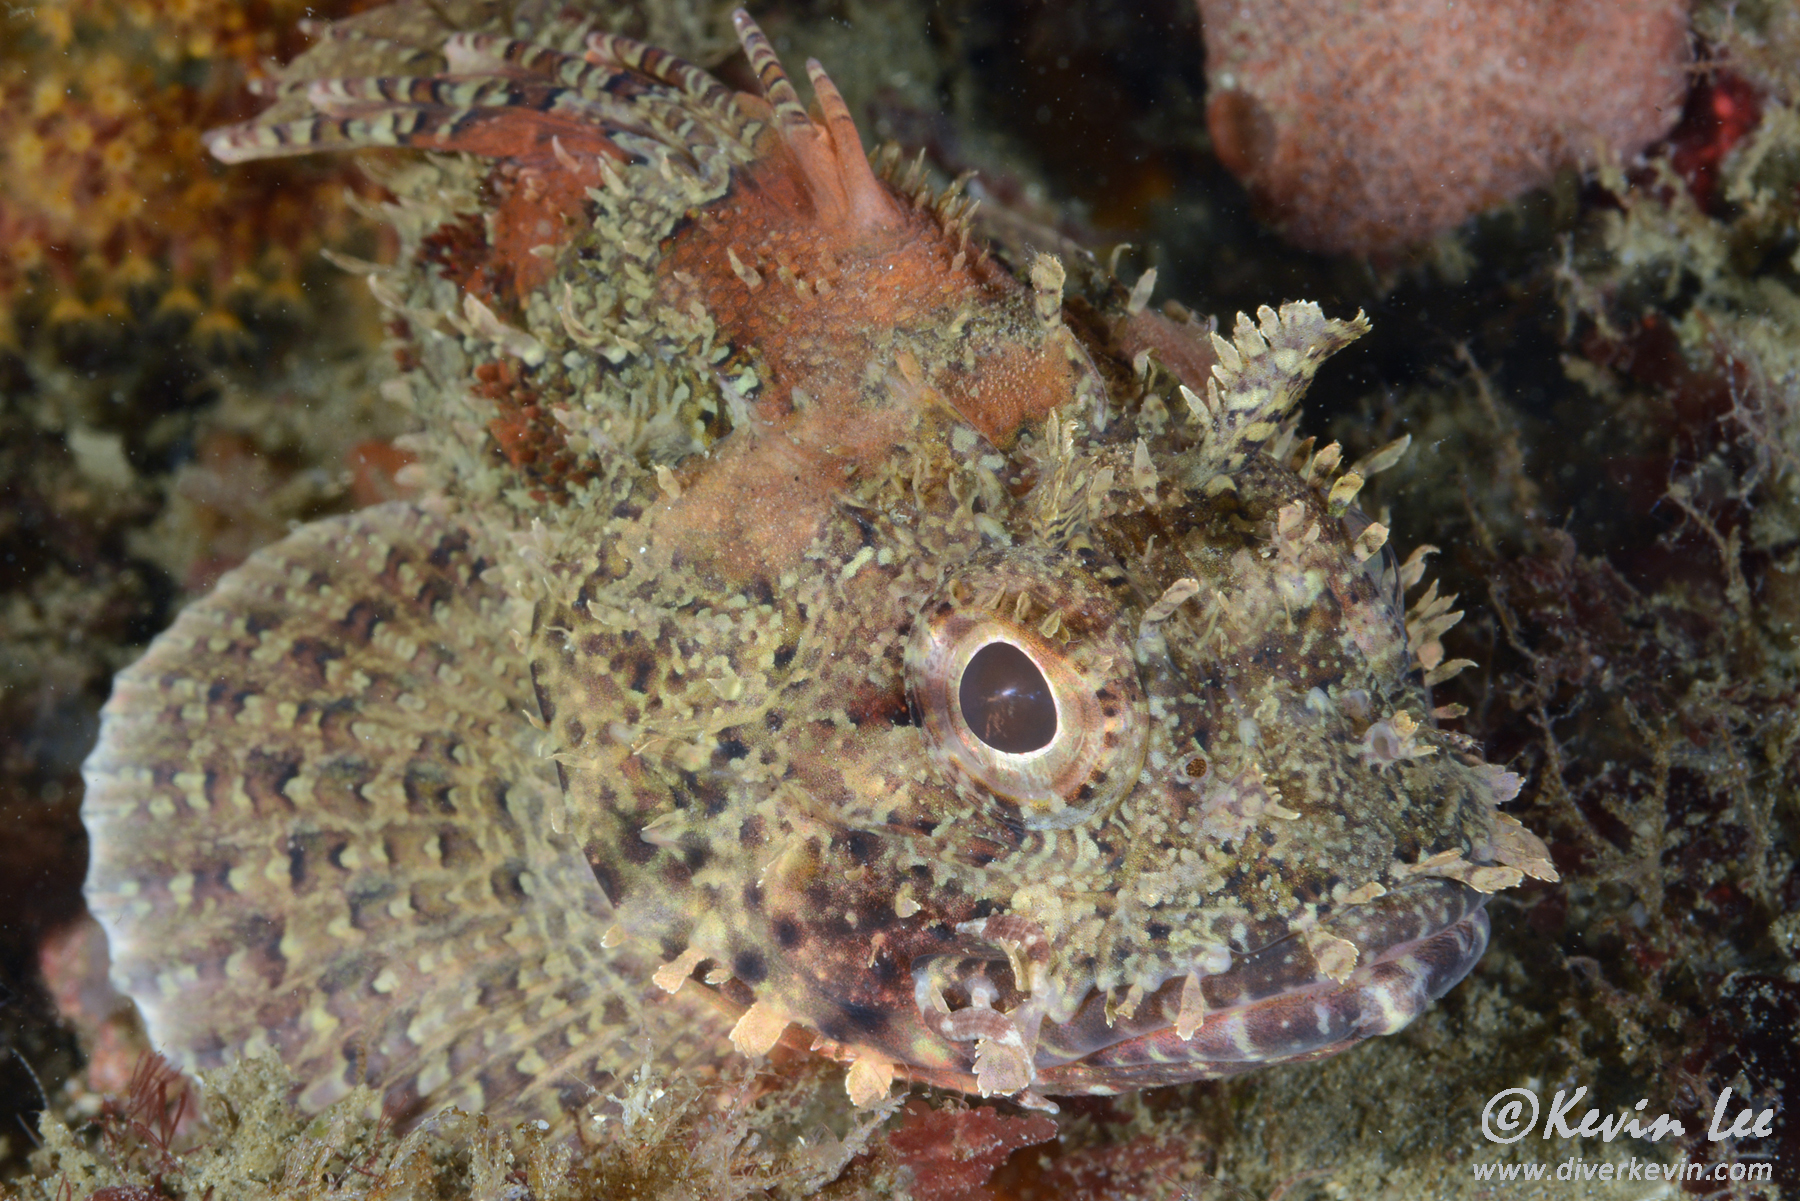
\includegraphics{cover_photo}~\\[1cm]
\pdftooltip{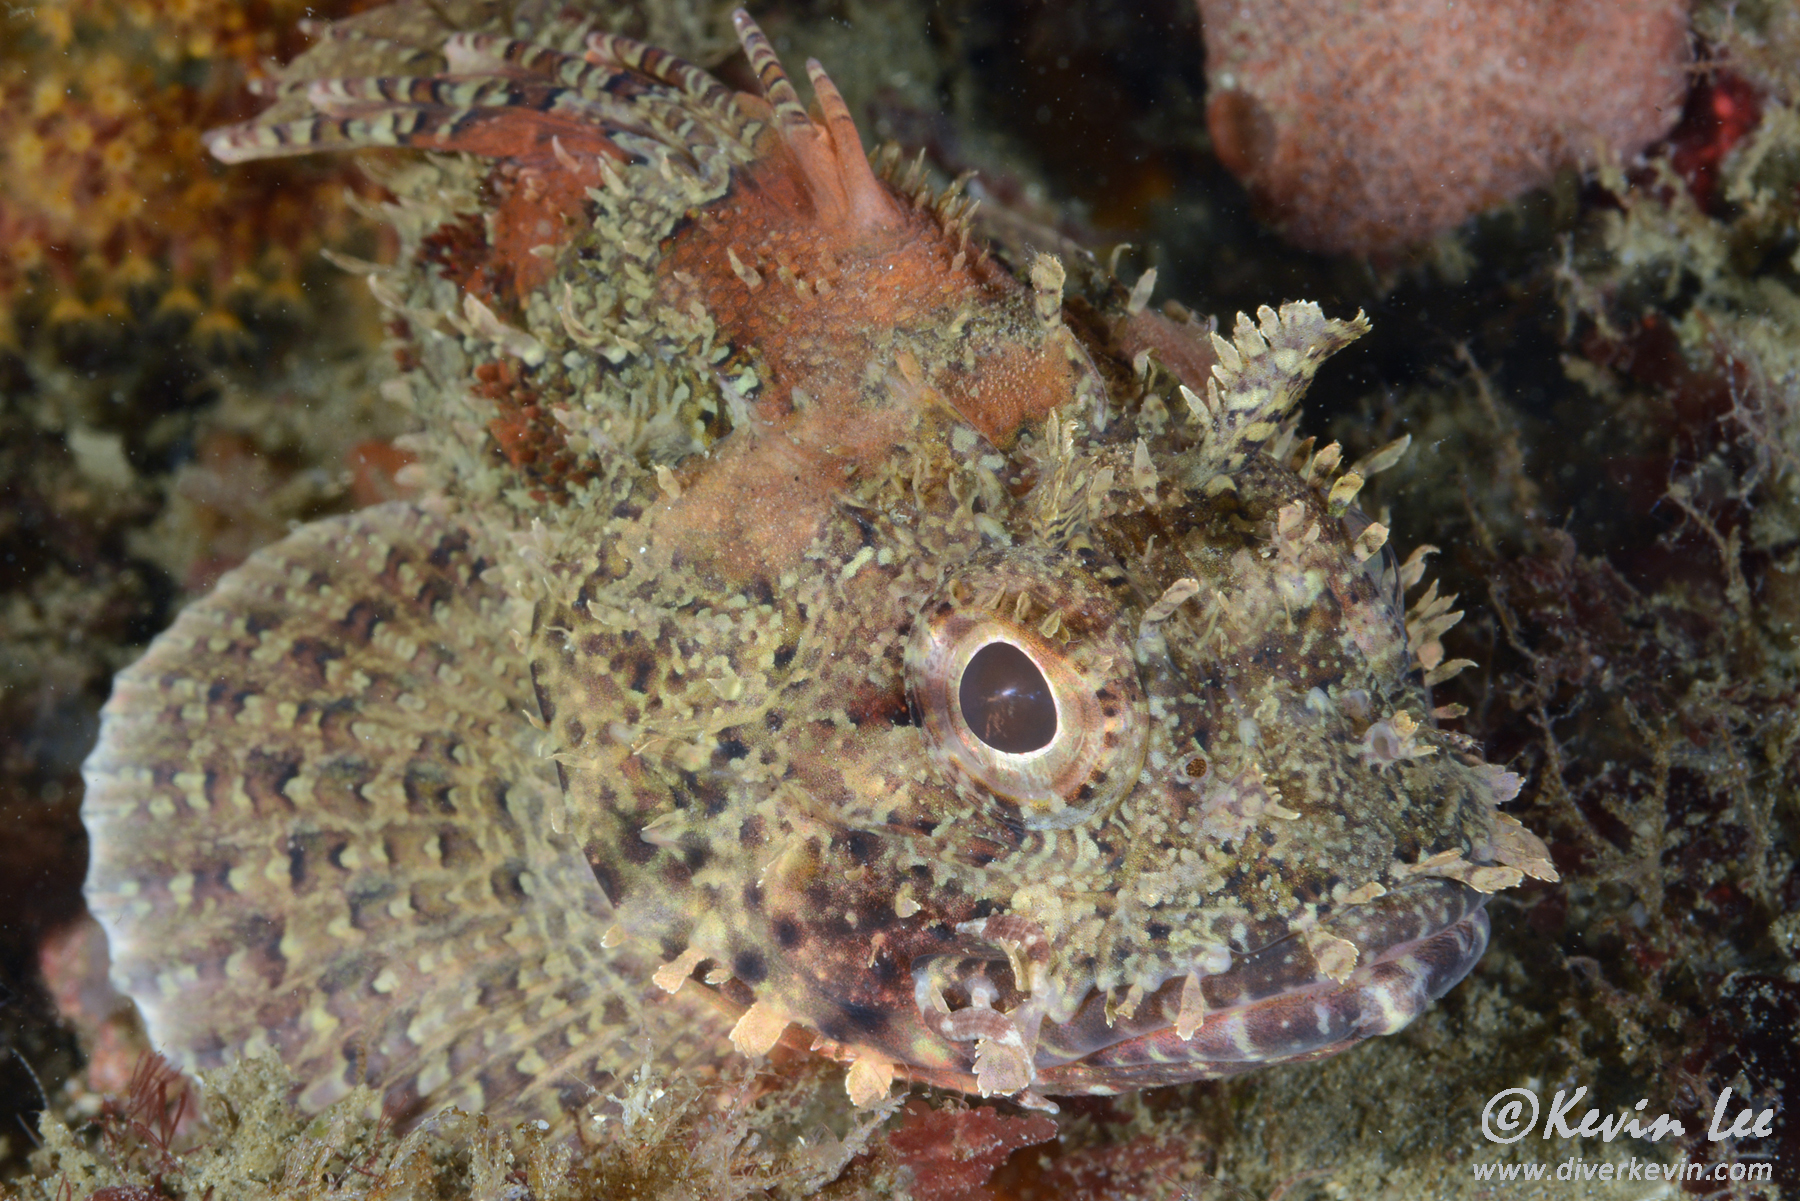
\includegraphics{cover_photo}}{This is a fish.}



Melissa H. Monk\textsuperscript{1}\\
Xi He\textsuperscript{1}\\
John Budrick\textsuperscript{2}\\

\vspace{.5cm}

\small
\textsuperscript{1}Southwest Fisheries Science Center, U.S. Department of Commerce, National Oceanic and Atmospheric Administration, National Marine Fisheries Service, 110 McAllister Road, Santa Cruz, California 95060\\

\vspace{.3cm}

\textsuperscript{2}California Department of Fish and Wildlife, 350 Harbor Blvd., Belmont, California 94002\\


\vspace{.5cm}

\vfill
Disclaimer: This information is distributed solely for the purpose of pre-dissemination
peer review under applicable information quality guidelines. It has not been formally
disseminated by NOAA Fisheries. It does not represent and should not be construed to
represent any agency determination or policy. 

\vspace{.3cm}
%Bottom of the page
%{\large \today}


\newpage

\begin{flushleft}
This report may be cited as:

Monk, M. H. ,He, X., and Budrick, J. 2017. Status of the California Scorpionfish (\emph{Scorpaena guttata}) Off Southern California in 2017. Pacific Fishery Management Council, Portland, OR. Available from http://www.pcouncil.org/groundfish/stock-assessments/
\end{flushleft}

\maketitle

\pagenumbering{roman}
\setcounter{page}{1}
\end{center}

{
\setcounter{tocdepth}{4}
\tableofcontents
}
\setlength{\parskip}{5mm plus1mm minus1mm} \pagebreak

\setcounter{page}{1} \renewcommand{\thefigure}{\alph{figure}}
\renewcommand{\thetable}{\alph{table}}

\section*{Executive Summary}\label{executive-summary}
\addcontentsline{toc}{section}{Executive Summary}

\subsection*{Stock}\label{stock}
\addcontentsline{toc}{subsection}{Stock}

This assessment reports the status of the California scorpionfish
(\emph{Scorpaena guttata}) resource in U.S. waters off the coast of
southern California (south of Pt. Conception) using data through 2016.
California scorpionfish are most abundant in the southern California
Bight and their range extends to Punta Eugena, Mexico, about halfway
down the Baja peninsula. Catches from Mexico were not included in this
assessment, and catches from Mexican waters that were landed in the U.S.
were excluded from the catch histories.

\subsection*{Catches}\label{catches}
\addcontentsline{toc}{subsection}{Catches}

Information on historical landings of California scorpionfish are
available back to 1916, with the assumption that from 1916 to 1968 all
of the commercial landings were caught by hook-and-line (Table
\ref{tab:Exec_catch}). Commercial landings were small during the years
of World War II, ranging between 16 to 63 metric tons (mt) per year. The
recreational fleets began ramping up in the 1960s and have dominated the
catch since then (Figures \ref{fig:Exec_catch1}-\ref{fig:Exec_catch2}).
The party/charter fleet has been the major component of the recreational
sector since the early 2000s.

The catches from the commercial fleets has been small in the last
decade, range from 1.19 to 4.54 mt per year (Figure
\ref{fig:r4ss_catches}). Since 2000, annual total landings of California
scorpionfish have ranged between 57-199 mt, with landings in 2016
totaling 74 mt.

California scorpionfish is not a major component of the commercial or
recreational fisheries in southern California. There has been little
discarding of the species in the commercial fisheries and the discard
mortality rate for the recreational fisheries is estimated to be 7\%.
The peak in discards from 2001-2005 was due to the closure of California
scorpionfish fishery between two and ten months of the year during that
period.

\FloatBarrier

\begin{figure}[htbp]
\centering
\includegraphics{California_scorpionfish_2017_files/figure-latex/unnamed-chunk-16-1.pdf}
\caption{California scorpionfish catch history for the recreational
fleets. \label{fig:Exec_catch1}}
\end{figure}

\begin{figure}[htbp]
\centering
\includegraphics{California_scorpionfish_2017_files/figure-latex/unnamed-chunk-17-1.pdf}
\caption{Stacked line plot of California scorpionfish catch history for
the commercial fleets. \label{fig:Exec_catch2}}
\end{figure}

\FloatBarrier

\begin{figure}[htbp]
\centering
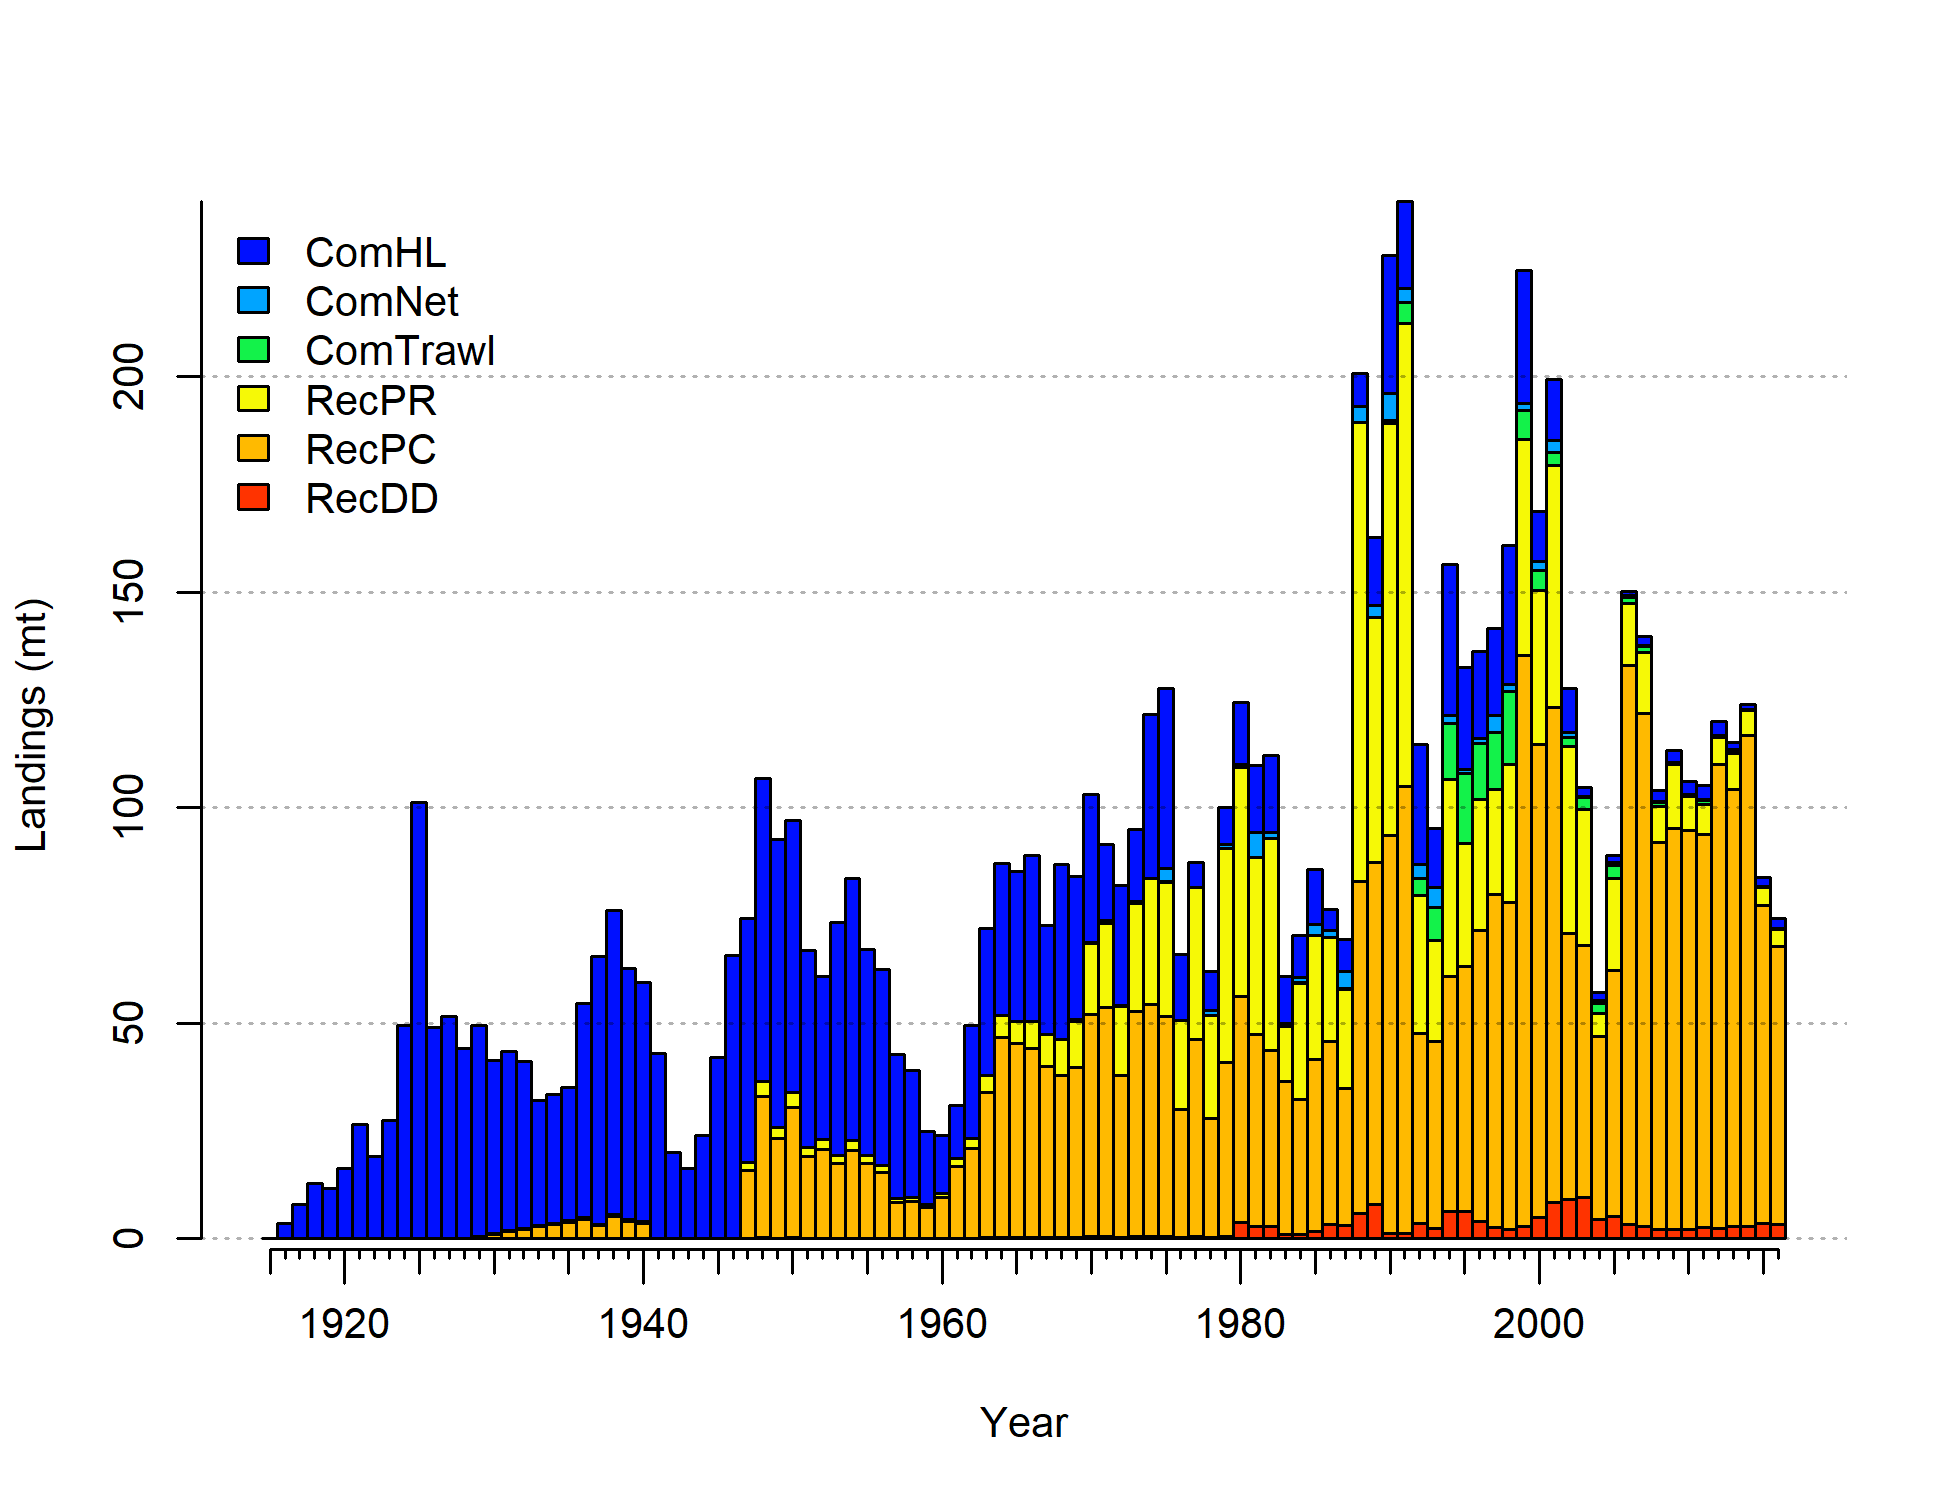
\includegraphics{r4ss/plots_mod1/catch2 landings stacked.png}
\caption{Catch history of California scorpionfish in the base model.
\label{fig:r4ss_catches}}
\end{figure}

\begin{table}[ht]
\centering
\caption{Recent California scorpionfish landings (mt) by 
                                            recreational (Rec.) and commercial (Com.) fleets.} 
\label{tab:Exec_catch}
\begin{tabular}{l>{\centering}p{.6in}>{\centering}p{1.1in}>{\centering}p{.9in}>{\centering}p{1.1in}>{\centering}p{.5in}>{\centering}p{.5in}>{\centering}p{.5in}}
  \hline
Year & Rec. Private & Rec. Party/Charter & Rec. Dead Discards & Com. Hook-and-line & Com. Trawl & Com. Gillnet & Total \\ 
  \hline
2007 & 14.24 & 118.87 & 2.89 & 1.90 & 1.48 & 0.21 & 139.58 \\ 
  2008 & 8.38 & 89.65 & 2.25 & 2.46 & 0.86 & 0.28 & 103.89 \\ 
  2009 & 14.68 & 93.16 & 2.09 & 2.97 & 0.27 & 0.13 & 113.31 \\ 
  2010 & 8.07 & 92.55 & 2.03 & 2.99 & 0.18 & 0.14 & 105.97 \\ 
  2011 & 6.84 & 91.18 & 2.66 & 3.24 & 1.05 & 0.24 & 105.21 \\ 
  2012 & 6.22 & 107.63 & 2.34 & 3.22 & 0.43 & 0.18 & 120.00 \\ 
  2013 & 8.18 & 101.31 & 2.94 & 1.73 & 0.83 & 0.14 & 115.14 \\ 
  2014 & 5.88 & 113.83 & 2.93 & 1.03 & 0.13 & 0.04 & 123.82 \\ 
  2015 & 4.15 & 73.78 & 3.59 & 2.21 & 0.13 & 0.03 & 83.89 \\ 
  2016 & 3.86 & 64.56 & 3.29 & 2.32 & 0.13 & 0.00 & 74.16 \\ 
   \hline
\end{tabular}
\end{table}

\FloatBarrier

\newpage

\subsection*{Data and Assessment}\label{data-and-assessment}
\addcontentsline{toc}{subsection}{Data and Assessment}

This a new full assessment for California scorpionfish, which was last
assessed in 2005 (Maunder et al.
\protect\hyperlink{ref-Maunder2005}{2005}) using Stock Synthesis II
version 1.18. This assessment uses the newest version of Stock Synthesis
(3.30.05). The model begins in 1916, and assumes the stock was at an
unfished equilibrium that year. In this assessment, aspects of the model
including landings, data, and modeling assumptions were re-evaluated.
The assessment was conducted using the length- and age-structured
modeling software Stock Synthesis (version 3.30.05.03). The population
was modeled allowing separate growth and mortality parameters for each
sex (a two-sex model) from 1916 to 2016, and forecast beyond 2016.

All of the data sources for California scorpionfish have been
re-evaluated for 2016, including the historical fishery catch-per-unit
effort time-series. The landings history has been updated and extended
back to 1916. Harvest was negligible prior to that year. Survey data
from five sources were used to develop indices of abundance: 1) Publicly
Owned Treatment Works (POTW) trawl surveys, 2) the NWFSC trawl survey,
3) a fishery-independent gill net survey, 4) the Southern California
Bight regional monitoring program trawl survey, and 5) the onboard
observer survey for retained catch. Length compositions were also
created for each fishery-dependent and -independent data source,
including a nuclear power generating station impingement survey that did
not have an associated index of abundance. Conditional age-at-length
information were available from the NWFSC trawl survey.

The definition of fishing fleets has changed from those in the 2005
assessment. Six fishing fleets were specified within this model: 1) a
combined commercial hook-and-line, fish pot, and ``other gear'' fleet,
2) the commercial gill net fleet, 3) the commercial trawl fleet, 4) the
recreational party/charter boat fleet (retained catch only), 5) the
recreational private boat fleet (retained catch only), and 6) a discard
fleet that combined the estimated discards from the recreational
party/charter and private boat fleets.

The assessment uses landings data; catch-per-unit-effort and survey
indices; length or age composition data for each year and fishery or
survey (with conditional age-at-length composition data for the NWFSC
trawl survey); information on weight-at-length; and estimates of ageing
error. Model outputs include recruitment at ``equilibrium spawning
output'', length-based selectivity of the fisheries and surveys,
retention of the fishery, catchability of the surveys, growth, the
time-series of spawning biomass, age and size structure, and current and
projected future stock status. Natural mortality and steepness were
fixed in the final model. This was done due to relatively flat
likelihood surfaces, such that fixing parameters and then varying them
in sensitivity analyses was deemed the best way to characterize
uncertainty.

Although there are many types of data available for California
scorpionfish since the 1980s which were used in this assessment, there
is little information about steepness and natural mortality. Estimates
of steepness are uncertain partly because of highly variable
recruitment. Uncertainty in natural mortality is common in many fish
stock assessments even when length and age data are available.

A number of sources of uncertainty are now addressed in this assessment.
This assessment includes gender differences in growth, an updated
length-weight curve, and new conditional length at age data. One of the
largest sources of uncertainty that is not considered in the current
model is the proportion of the stock in Mexico and the connectivity
between the portion of the fishery in Mexican and U.S. waters.

A base model was selected which best captures the central tendency for
those sources of uncertainty considered in the model for the California
scorpionfish stock in southern California (Figure
\ref{fig:assess_region_map}).

\begin{figure}[htbp]
\centering
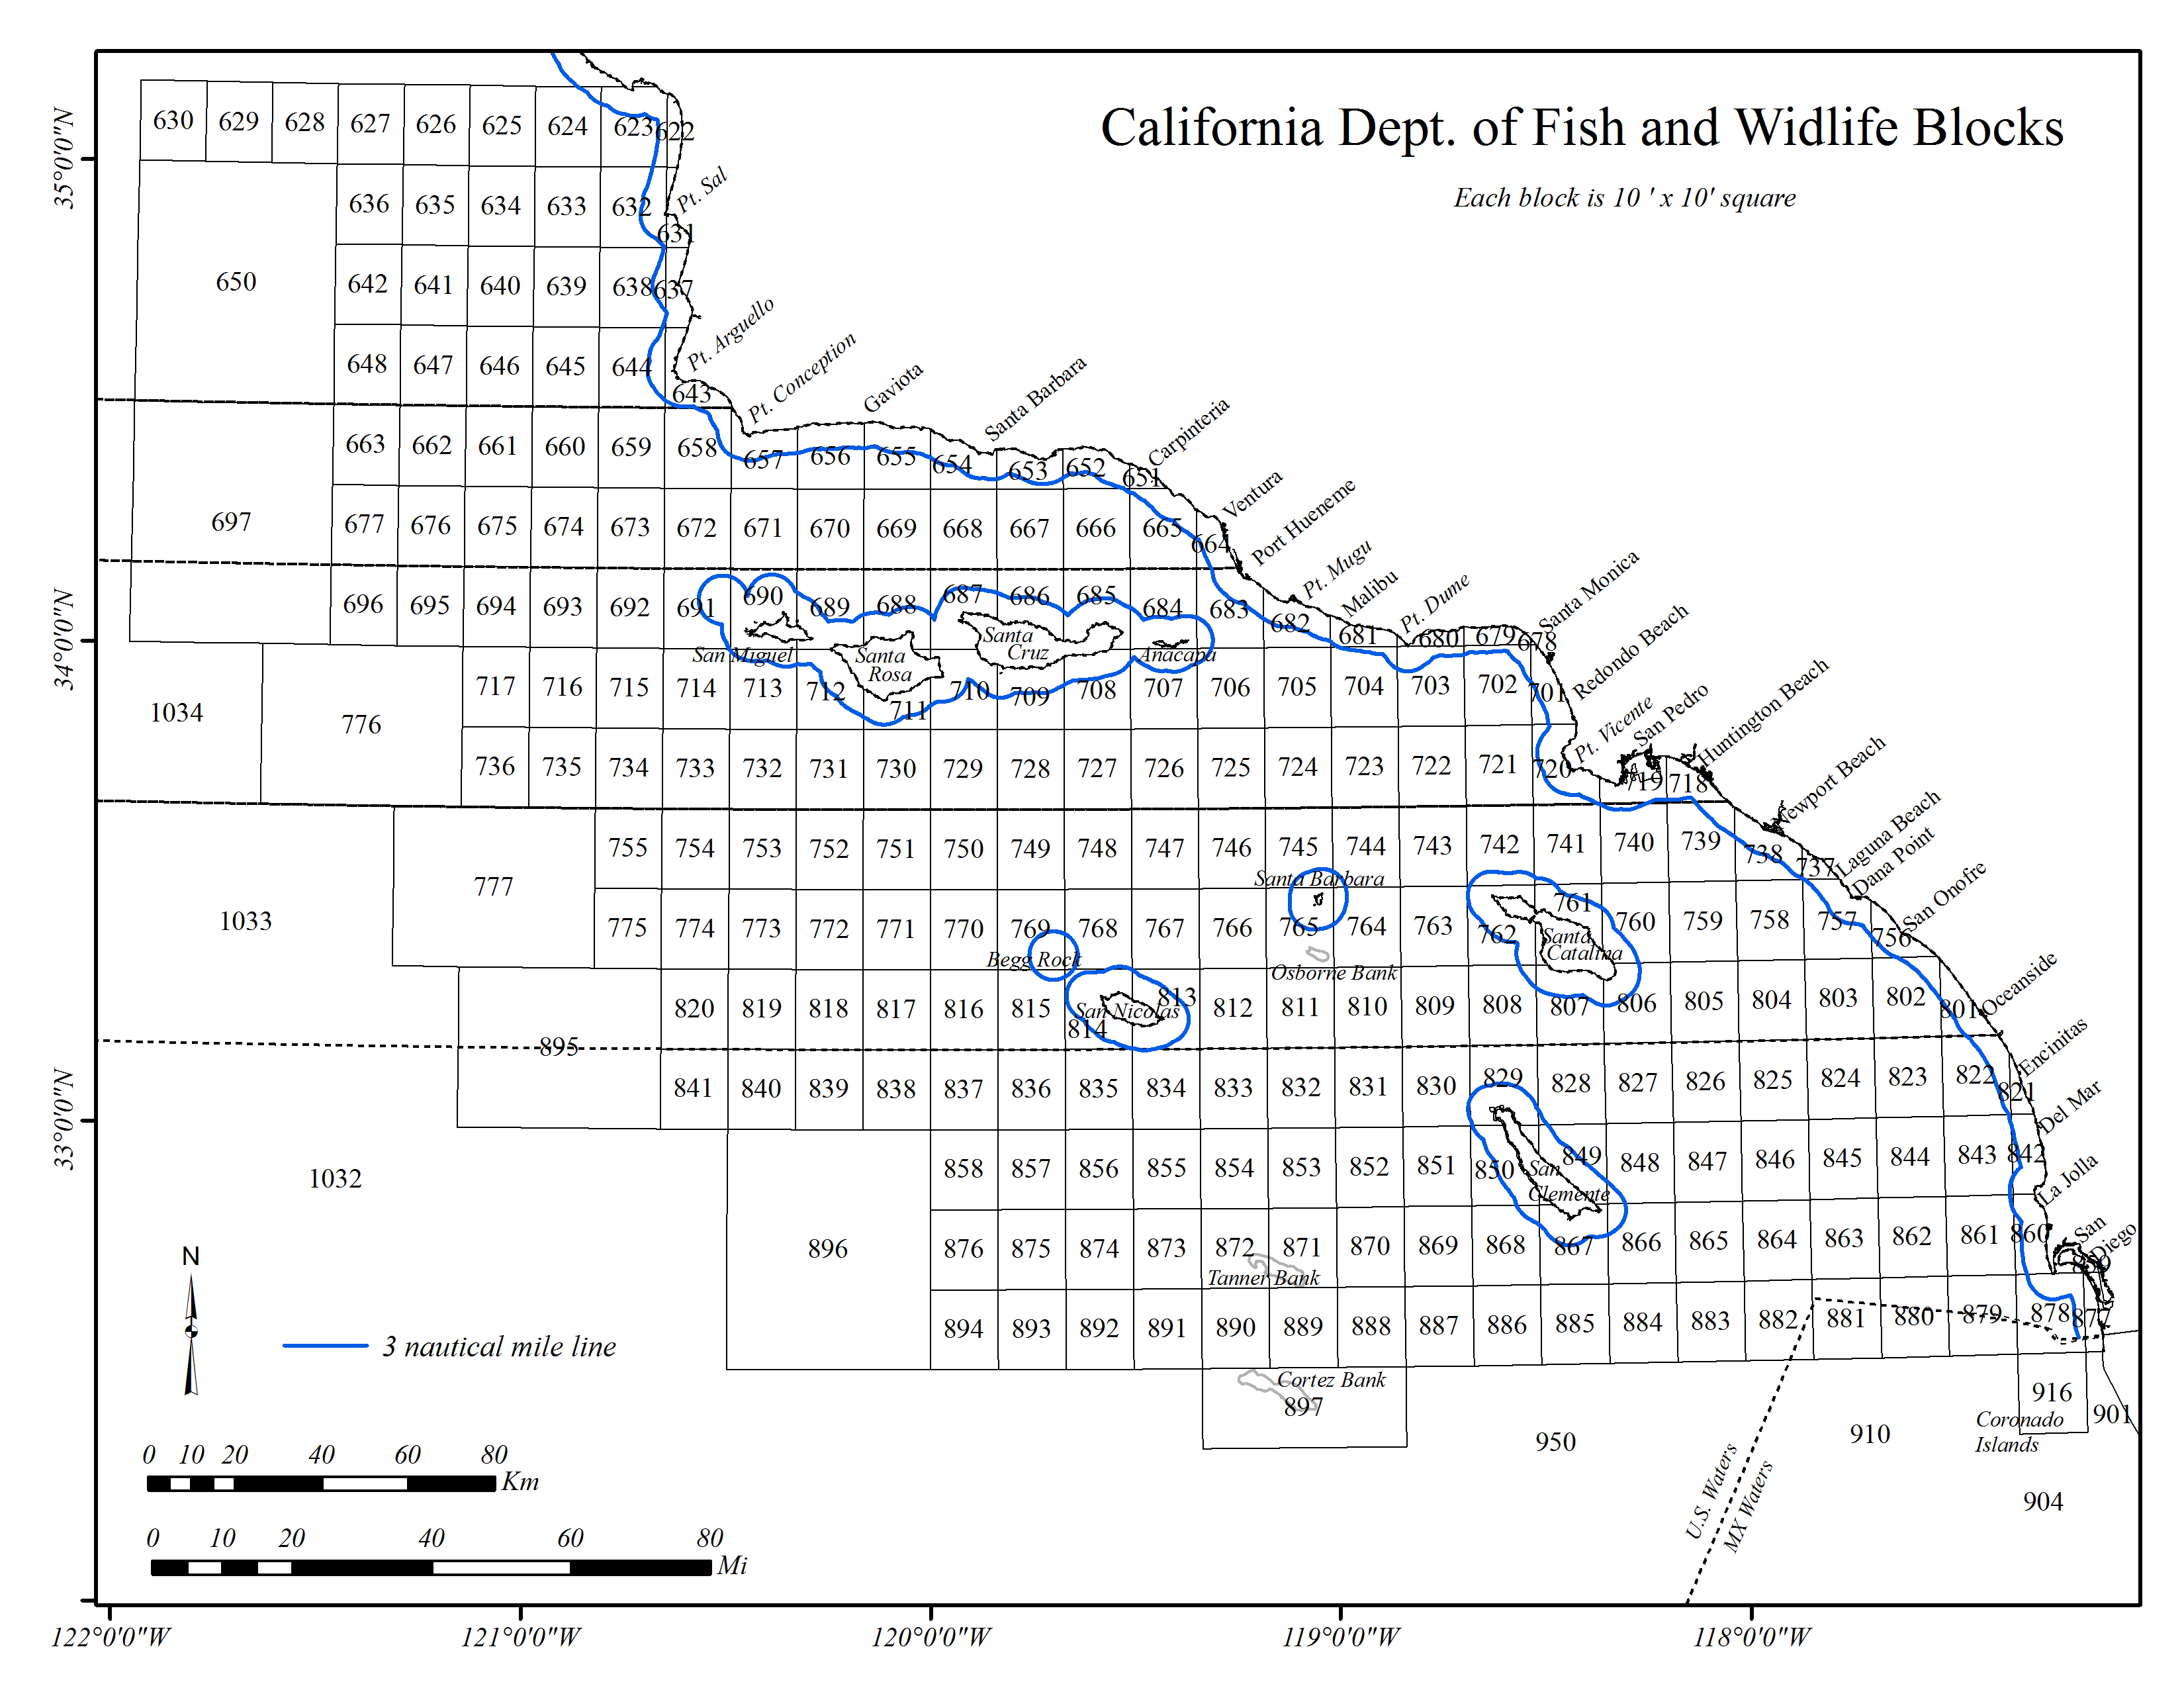
\includegraphics{Figures/assess_region_map.png}
\caption{Map depicting the distribution of California scorpionfish out
to 600 ft. The stock assessment is bounded at Pt. Conception in the
north to the U.S./Mexico border in the south.
\label{fig:assess_region_map}}
\end{figure}

\FloatBarrier

\subsection*{Stock Biomass}\label{stock-biomass}
\addcontentsline{toc}{subsection}{Stock Biomass}

The predicted spawning biomass from the base model generally showed a
slight decline prior to 1965, when information on recruitment
variability became available (Figure \ref{fig:Spawnbio_all} and Table
\ref{tab:SpawningDeplete_mod1}). A short, but sharp decline occurred
between 1965 and 1985, followed by a period cyclical variation in
spawning biomass, and then a decline from 2000 to 2015. The stock showed
increases in stock size in 2015 due to a combination of strong
recruitment and smaller catches in 2015 and 2016. The 2016 estimated
spawning biomass relative to unfished equilibrium spawning biomass is
above the target of 40\% of unfished spawning biomass at 54.3\% (95\%
asymptotic interval: \(\pm\) 43\%-65.7\%) (Figure
\ref{fig:RelDeplete_all}). Approximate confidence intervals based on the
asymptotic variance estimates show that the uncertainty in the estimated
spawning biomass is high.

\FloatBarrier

\begin{table}[ht]
\centering
\caption{Recent trend in beginning of the 
                                      year spawning biomass and depletion for
                                      the base model for California scorpionfish.} 
\label{tab:SpawningDeplete_mod1}
\begin{tabular}{l>{\centering}p{1.3in}>{\centering}p{1.2in}>{\centering}p{1in}>{\centering}p{1.2in}}
  \hline
Year & Spawning biomass (mt) & 95\% confidence interval & Estimated depletion & 95\% confidence interval \\ 
  \hline
2008 & 1144.500 & (654.46-1634.54) & 0.705 & (0.573-0.836) \\ 
  2009 & 1090.480 & (629.78-1551.18) & 0.671 & (0.55-0.793) \\ 
  2010 & 1029.330 & (597.2-1461.46) & 0.634 & (0.521-0.746) \\ 
  2011 & 980.130 & (571.79-1388.47) & 0.603 & (0.5-0.707) \\ 
  2012 & 943.555 & (553.81-1333.3) & 0.581 & (0.485-0.677) \\ 
  2013 & 890.084 & (518.85-1261.32) & 0.548 & (0.456-0.64) \\ 
  2014 & 810.223 & (462.86-1157.59) & 0.499 & (0.41-0.587) \\ 
  2015 & 746.227 & (412.08-1080.38) & 0.459 & (0.371-0.548) \\ 
  2016 & 774.813 & (426.28-1123.35) & 0.477 & (0.381-0.572) \\ 
  2017 & 882.457 & (484.21-1280.71) & 0.543 & (0.43-0.657) \\ 
   \hline
\end{tabular}
\end{table}

\FloatBarrier

\begin{figure}[htbp]
\centering
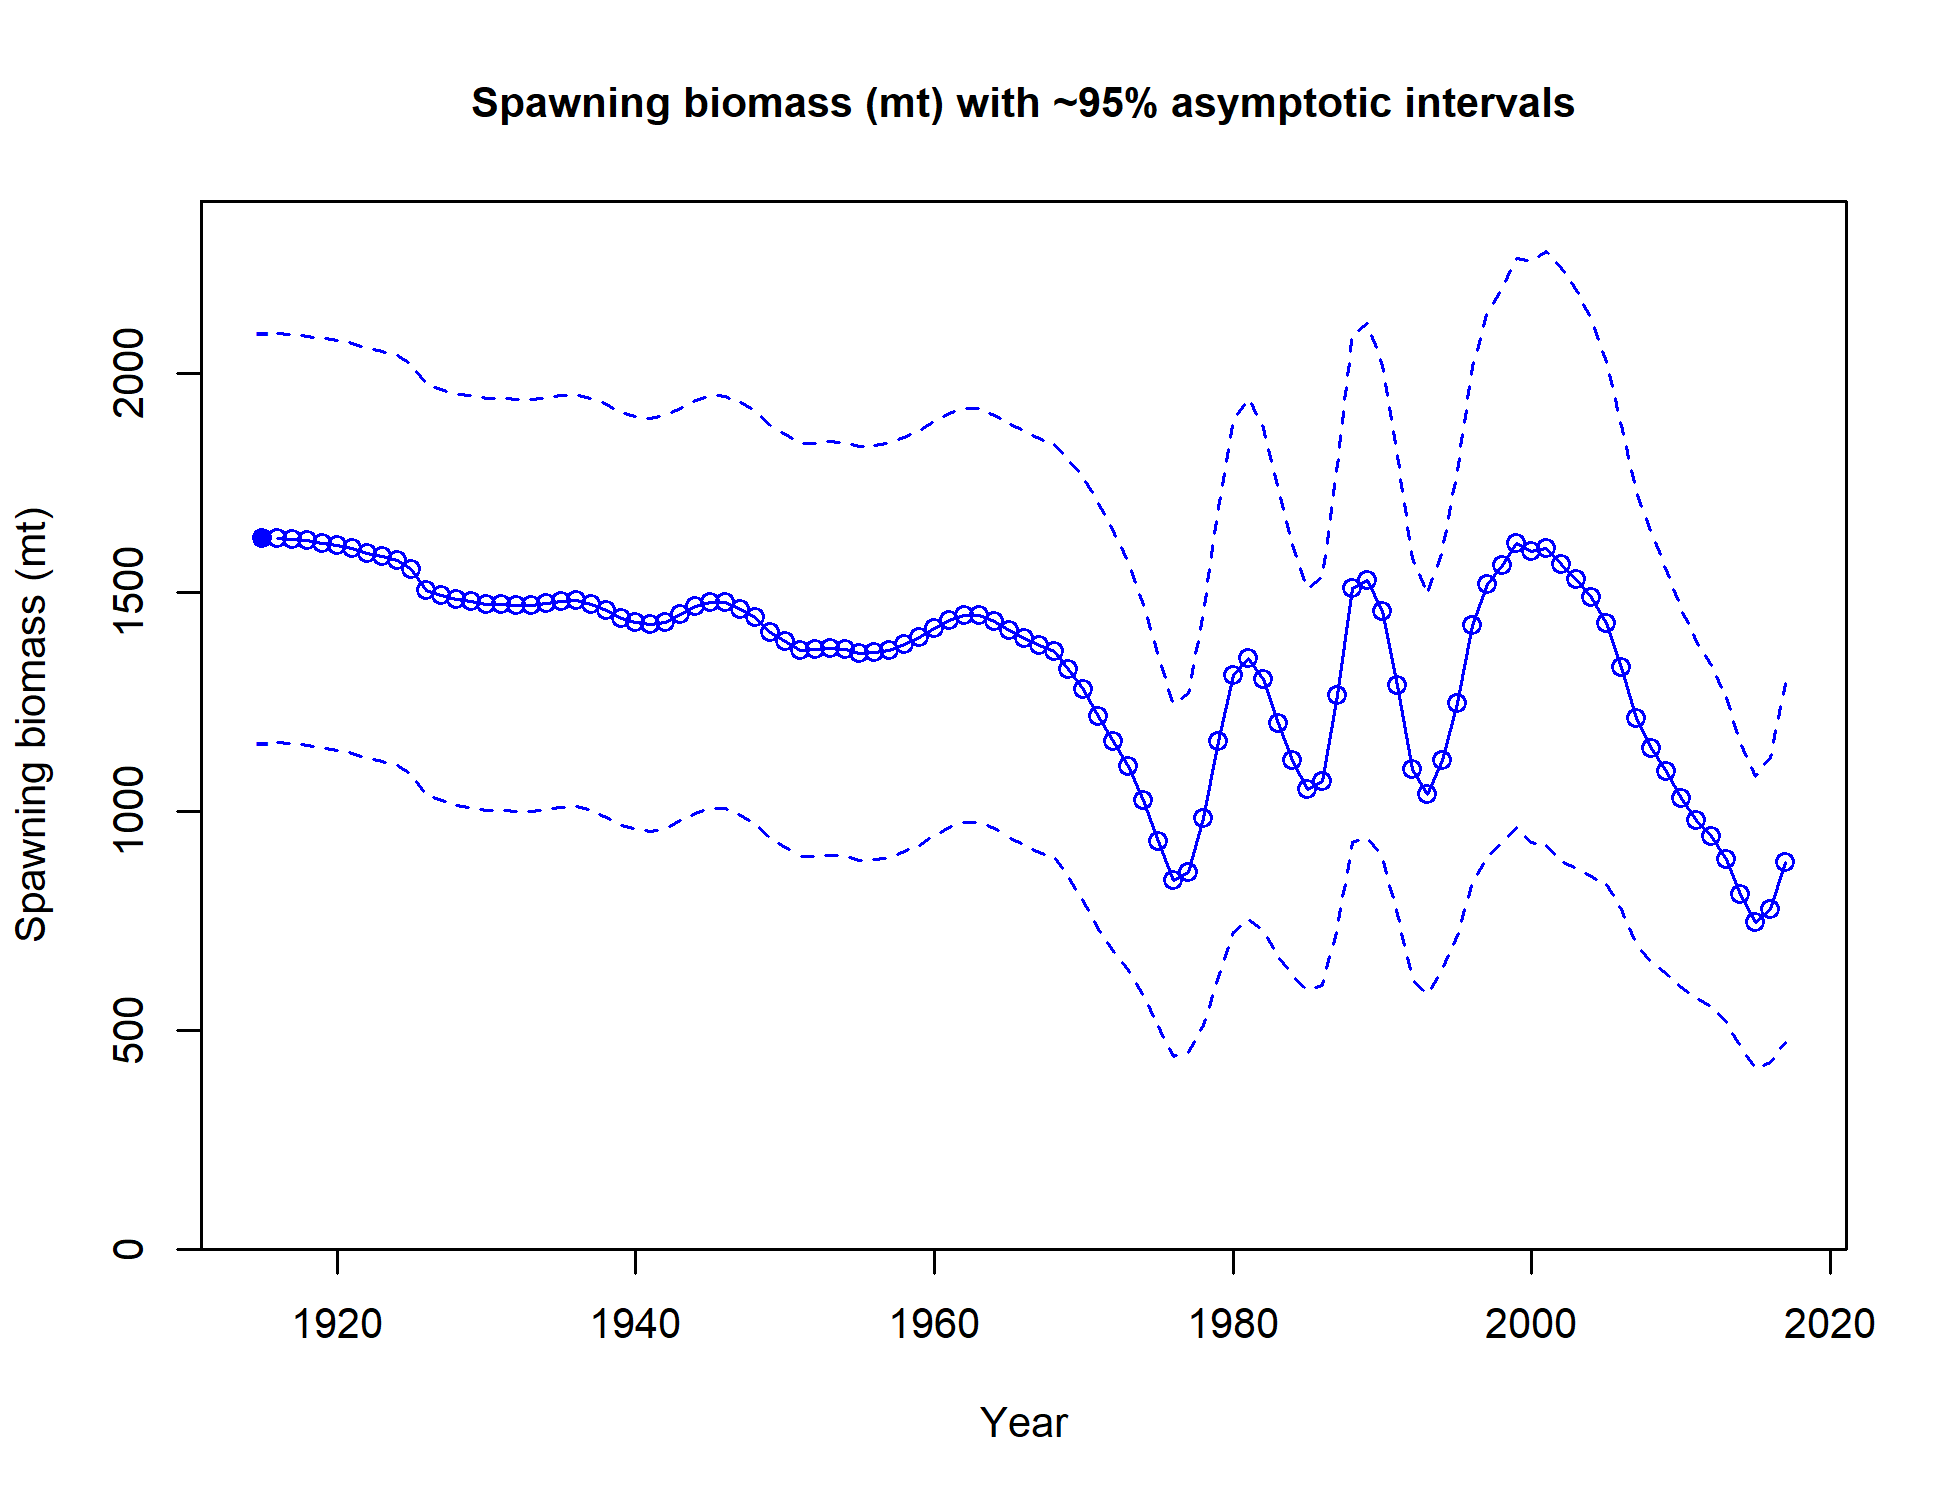
\includegraphics{r4ss/plots_mod1/ts7_Spawning_biomass_(mt)_with_95_asymptotic_intervals_intervals.png}
\caption{Time series of spawning biomass trajectory (circles and line:
median; light broken lines: 95\% credibility intervals) for the base
case assessment model. \label{fig:Spawnbio_all}}
\end{figure}

\begin{figure}[htbp]
\centering
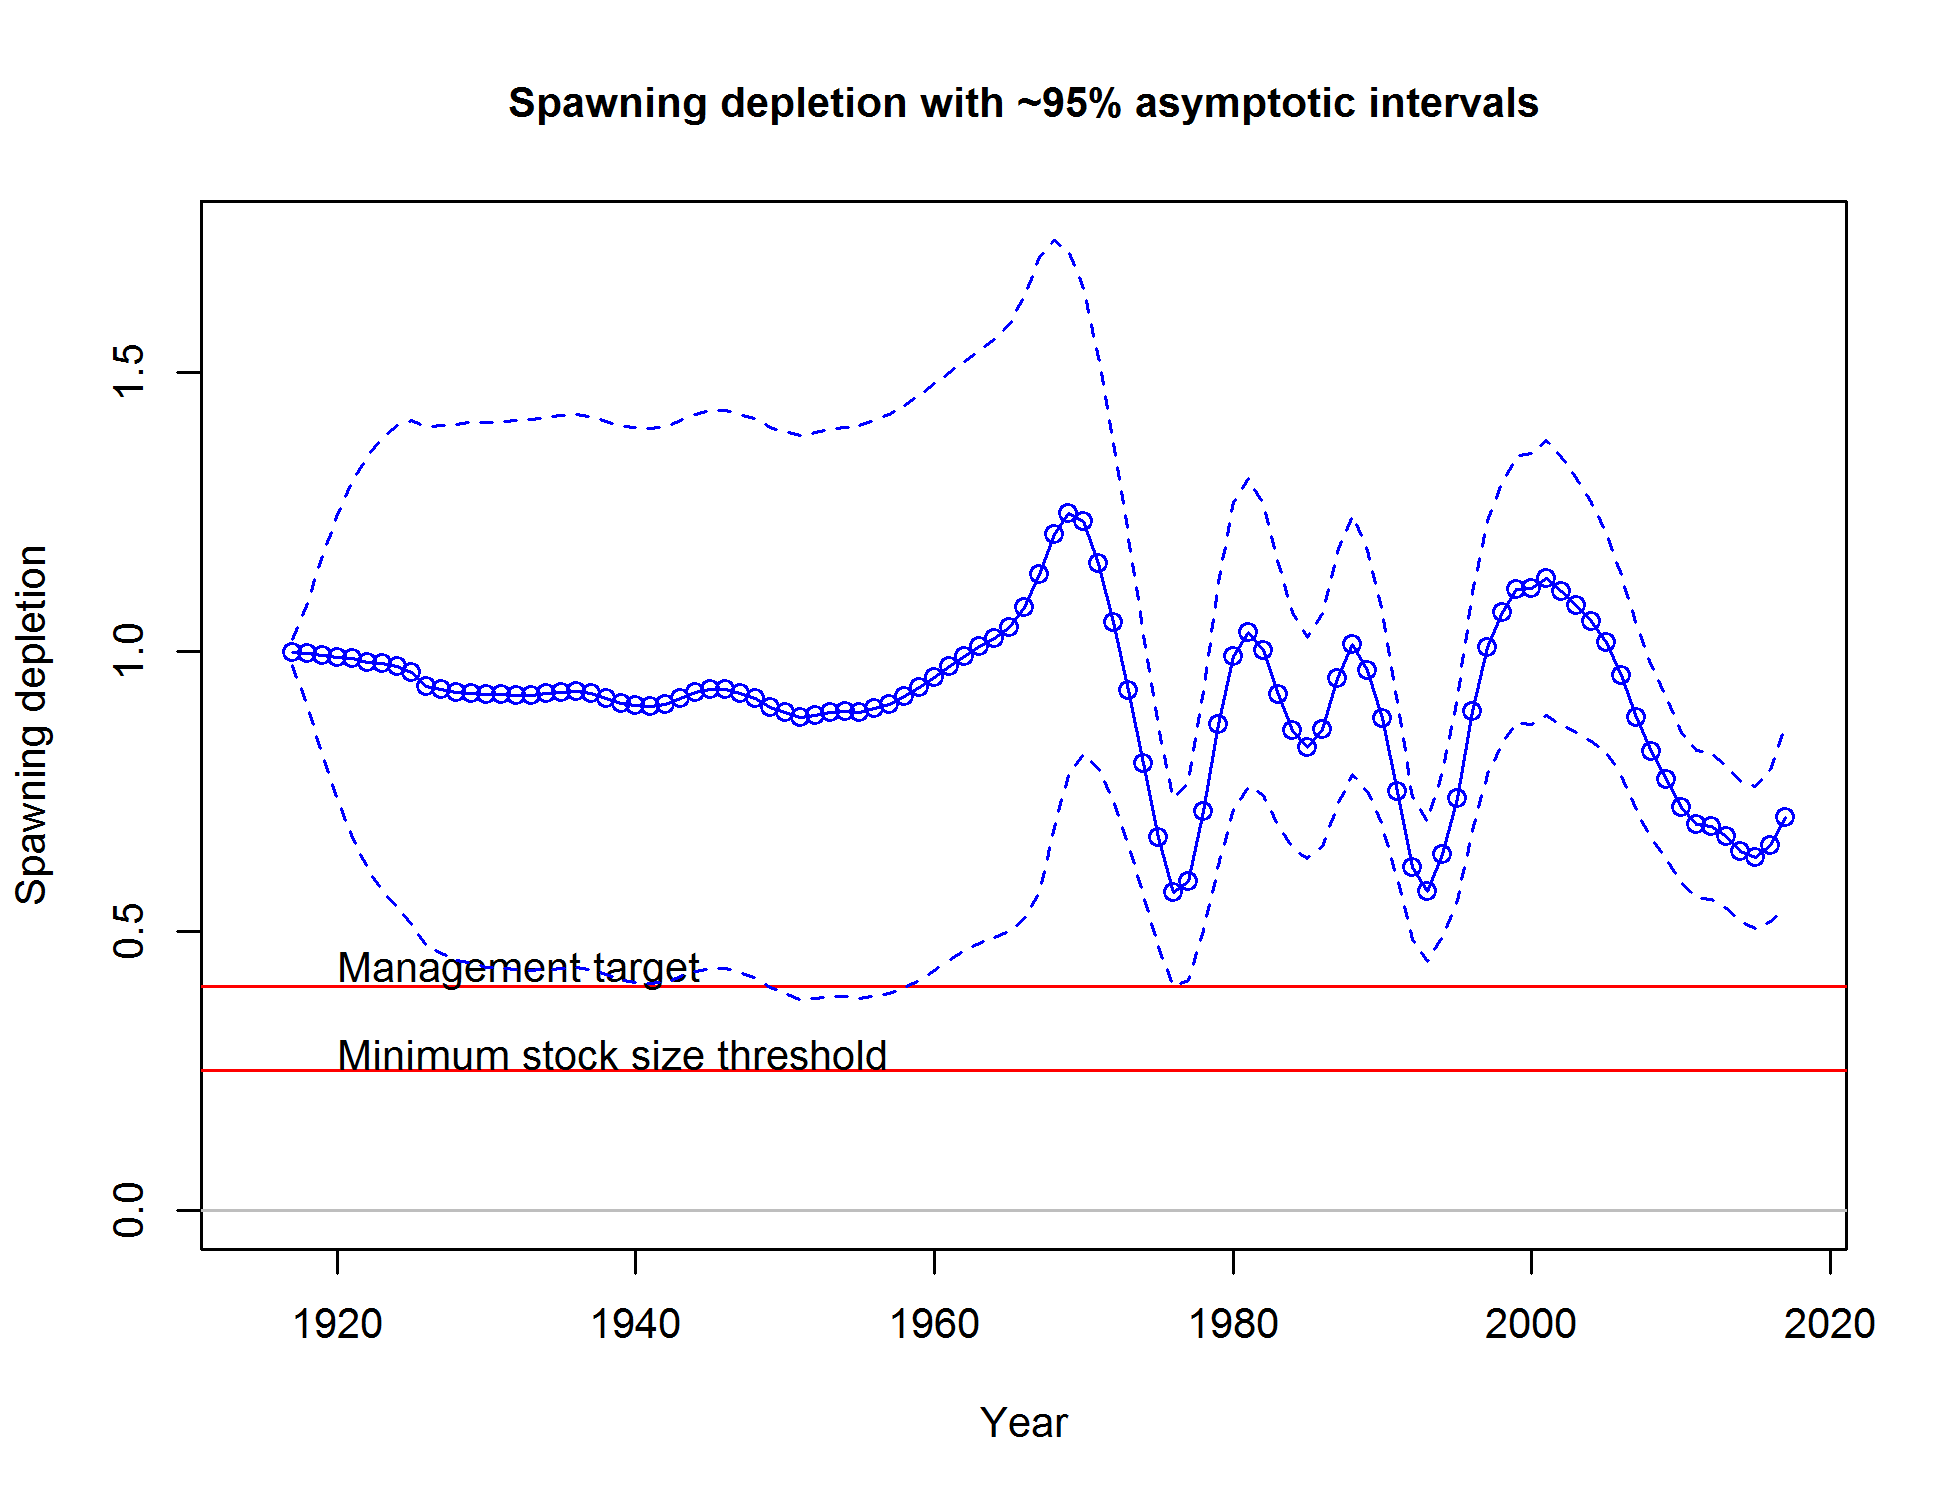
\includegraphics{r4ss/plots_mod1/ts9_Spawning_depletion_with_95_asymptotic_intervals_intervals.png}
\caption{Estimated relative depletion with approximate 95\% asymptotic
confidence intervals (dashed lines) for the base case assessment model.
\label{fig:RelDeplete_all}}
\end{figure}

\FloatBarrier

\subsection*{Recruitment}\label{recruitment}
\addcontentsline{toc}{subsection}{Recruitment}

Recruitment deviations were estimated from 1965-2016 (Figure
\ref{fig:Recruits_all} and Table \ref{tab:Recruit_mod1}). Historically,
there are estimates of large recruitment from 1975-1977, 1984-1985 and
in 1993 and 1996. There is early evidence of a strong recruitment in
2013. The four lowest recruitment estimated within the model (in
ascending order) occurred in 2012, 2011, 1989, and 1988.

\begin{table}[ht]
\centering
\caption{Recent recruitment for the base model.} 
\label{tab:Recruit_mod1}
\begin{tabular}{>{\centering}p{.8in}>{\centering}p{1.6in}>{\centering}p{2in}}
  \hline
Year & Estimated Recruitment (1,000s) & 95\% confidence interval \\ 
  \hline
2008 & 2288.15 & (1198.27 - 4369.33) \\ 
  2009 & 2589.07 & (1388.65 - 4827.18) \\ 
  2010 & 2483.75 & (1330.55 - 4636.43) \\ 
  2011 & 1178.81 & (541.36 - 2566.83) \\ 
  2012 & 1112.10 & (509.72 - 2426.35) \\ 
  2013 & 3747.47 & (2048.29 - 6856.23) \\ 
  2014 & 3529.05 & (1626.81 - 7655.6) \\ 
  2015 & 7585.54 & (3389.96 - 16973.8) \\ 
  2016 & 3268.02 & (1063.03 - 10046.74) \\ 
  2017 & 3343.81 & (1088.44 - 10272.52) \\ 
   \hline
\end{tabular}
\end{table}

\FloatBarrier

\begin{figure}[htbp]
\centering
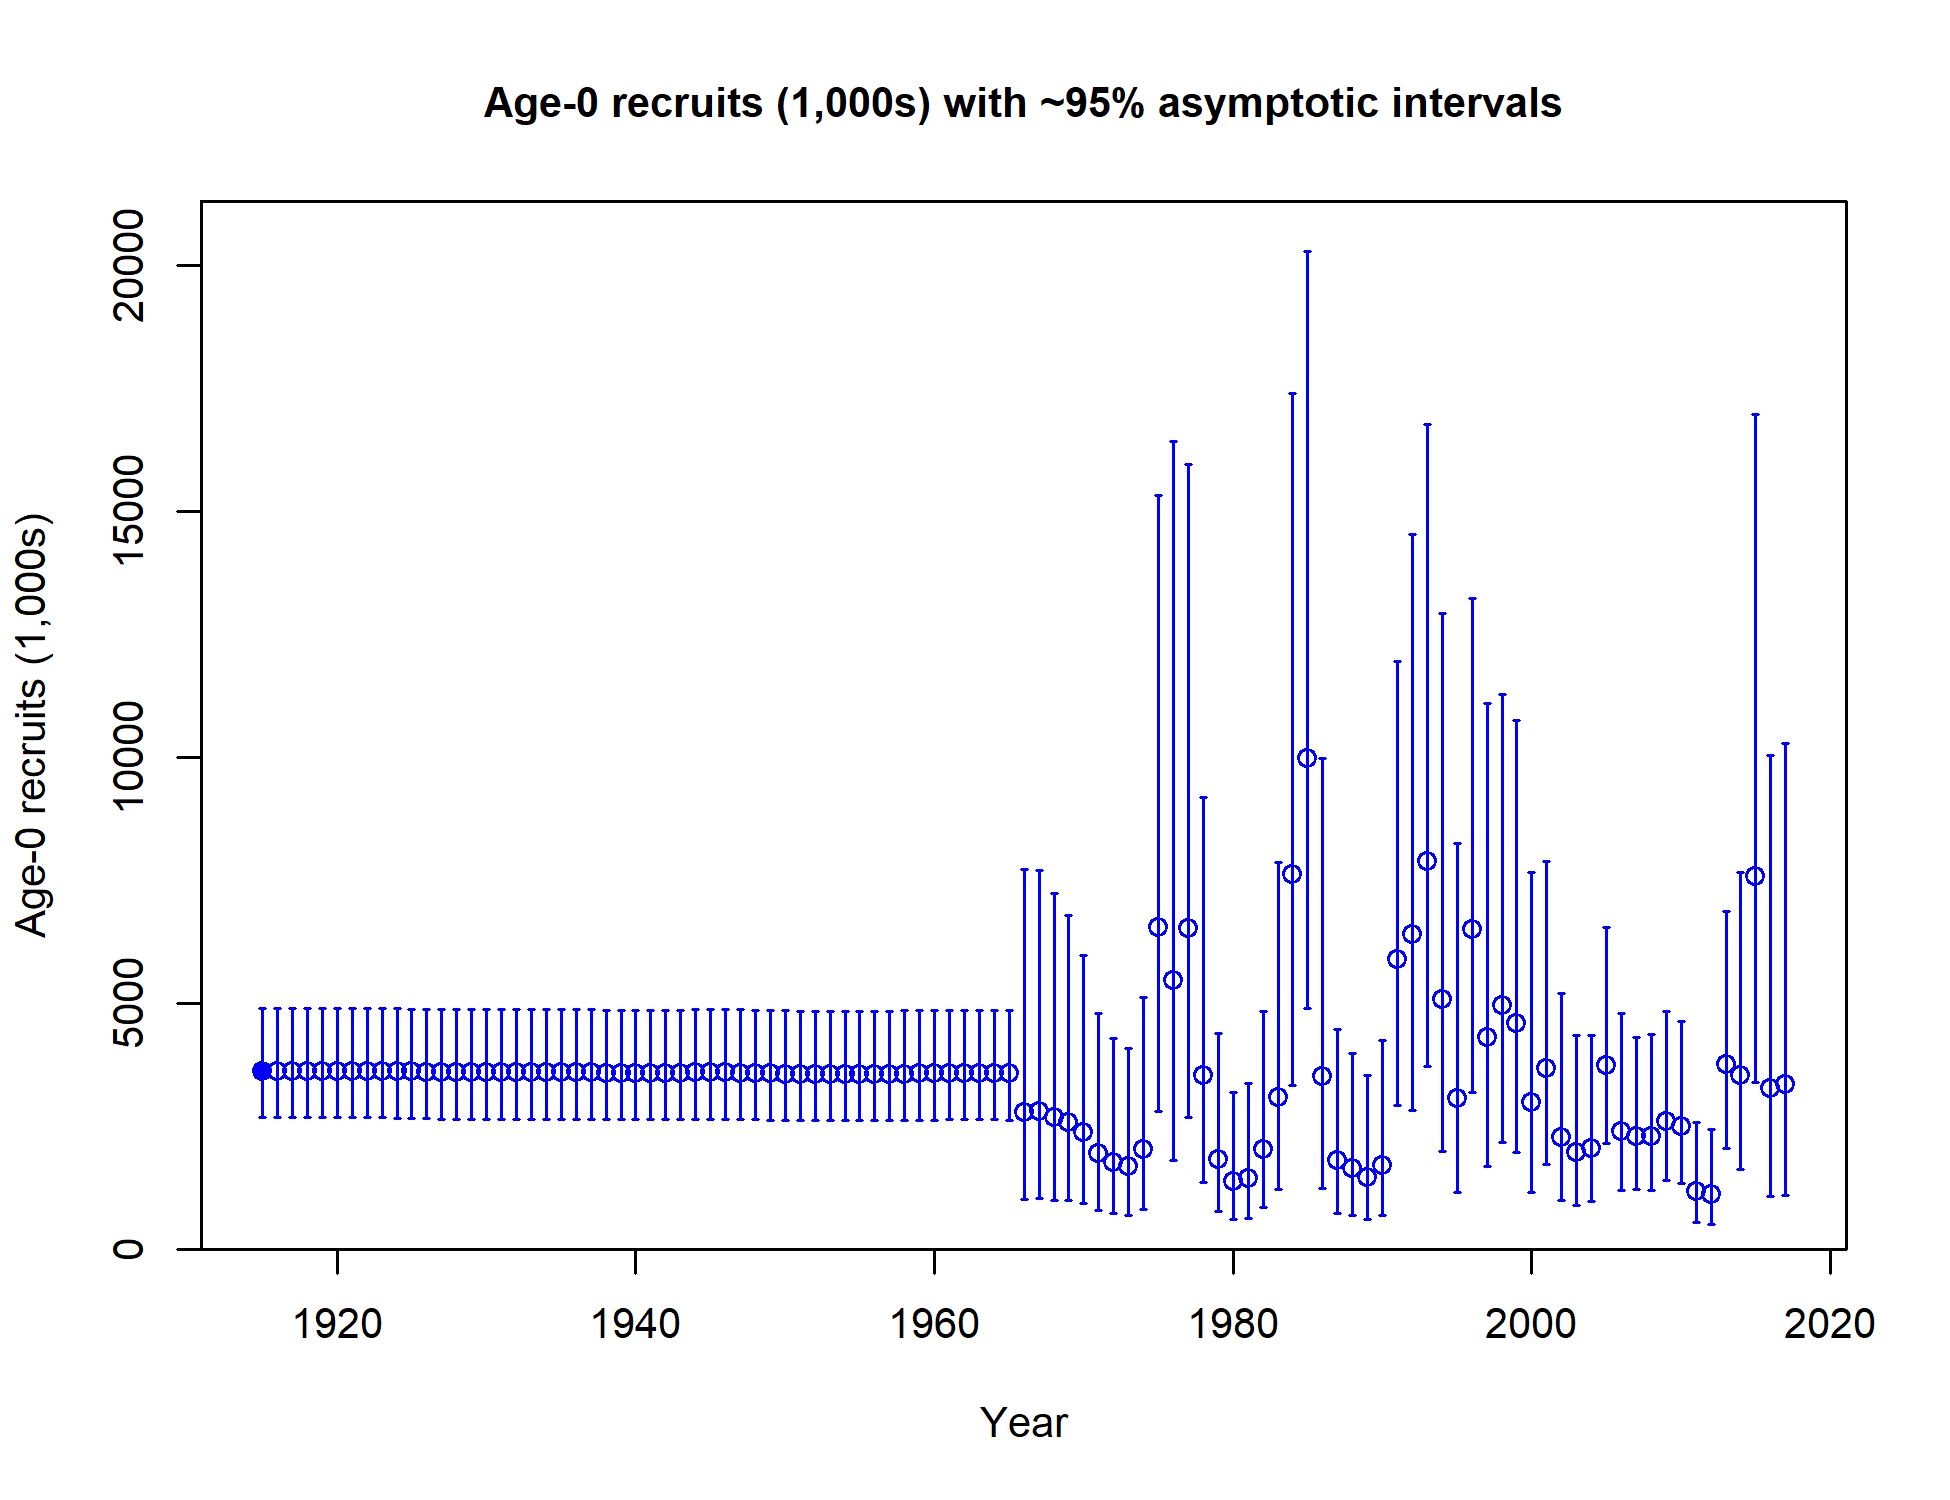
\includegraphics{r4ss/plots_mod1/ts11_Age-0_recruits_(1000s)_with_95_asymptotic_intervals.png}
\caption{Time series of estimated California scorpionfish recruitments
for the base-case model with 95\% confidence or credibility intervals.
\label{fig:Recruits_all}}
\end{figure}

\FloatBarrier

\subsection*{Exploitation status}\label{exploitation-status}
\addcontentsline{toc}{subsection}{Exploitation status}

Harvest rates estimated by the base model have never exceeded management
target levels (Table \ref{tab:SPR_Exploit_mod1} and Figure
\ref{fig:SPR_all}). Recent harvest rates have been relatively constant
for the last decade. The estimated relative depletion is currently
greater than the 40\% unfished spawning output target. Recent
exploitation rates on California scorpionfish were predicted to be
significantly below target levels.

\FloatBarrier

\begin{table}[ht]
\centering
\caption{Recent trend in spawning potential 
                                        ratio (entered as $(1-SPR)/(1-SPR_{50\%})$) 
                                        and exploitation for California scorpionfish in the base model.} 
\label{tab:SPR_Exploit_mod1}
\begin{tabular}{l>{\centering}p{1in}>{\centering}p{1.2in}>{\centering}p{1in}>{\centering}p{1.2in}}
  \hline
Year & Estimated (1-SPR)/(1-SPR50\%) & 95\% confidence interval & Harvest rate (ratio) & 95\% confidence interval \\ 
  \hline
2007 & 0.50 & (0.33-0.66) & 0.06 & (0.04-0.08) \\ 
  2008 & 0.43 & (0.27-0.58) & 0.05 & (0.03-0.07) \\ 
  2009 & 0.47 & (0.31-0.63) & 0.06 & (0.03-0.08) \\ 
  2010 & 0.47 & (0.31-0.63) & 0.05 & (0.03-0.08) \\ 
  2011 & 0.49 & (0.32-0.65) & 0.06 & (0.03-0.08) \\ 
  2012 & 0.55 & (0.38-0.73) & 0.07 & (0.04-0.09) \\ 
  2013 & 0.56 & (0.38-0.74) & 0.07 & (0.04-0.1) \\ 
  2014 & 0.61 & (0.43-0.8) & 0.08 & (0.05-0.11) \\ 
  2015 & 0.50 & (0.33-0.67) & 0.05 & (0.03-0.08) \\ 
  2016 & 0.47 & (0.3-0.64) & 0.04 & (0.02-0.06) \\ 
   \hline
\end{tabular}
\end{table}

\FloatBarrier

\begin{figure}[htbp]
\centering
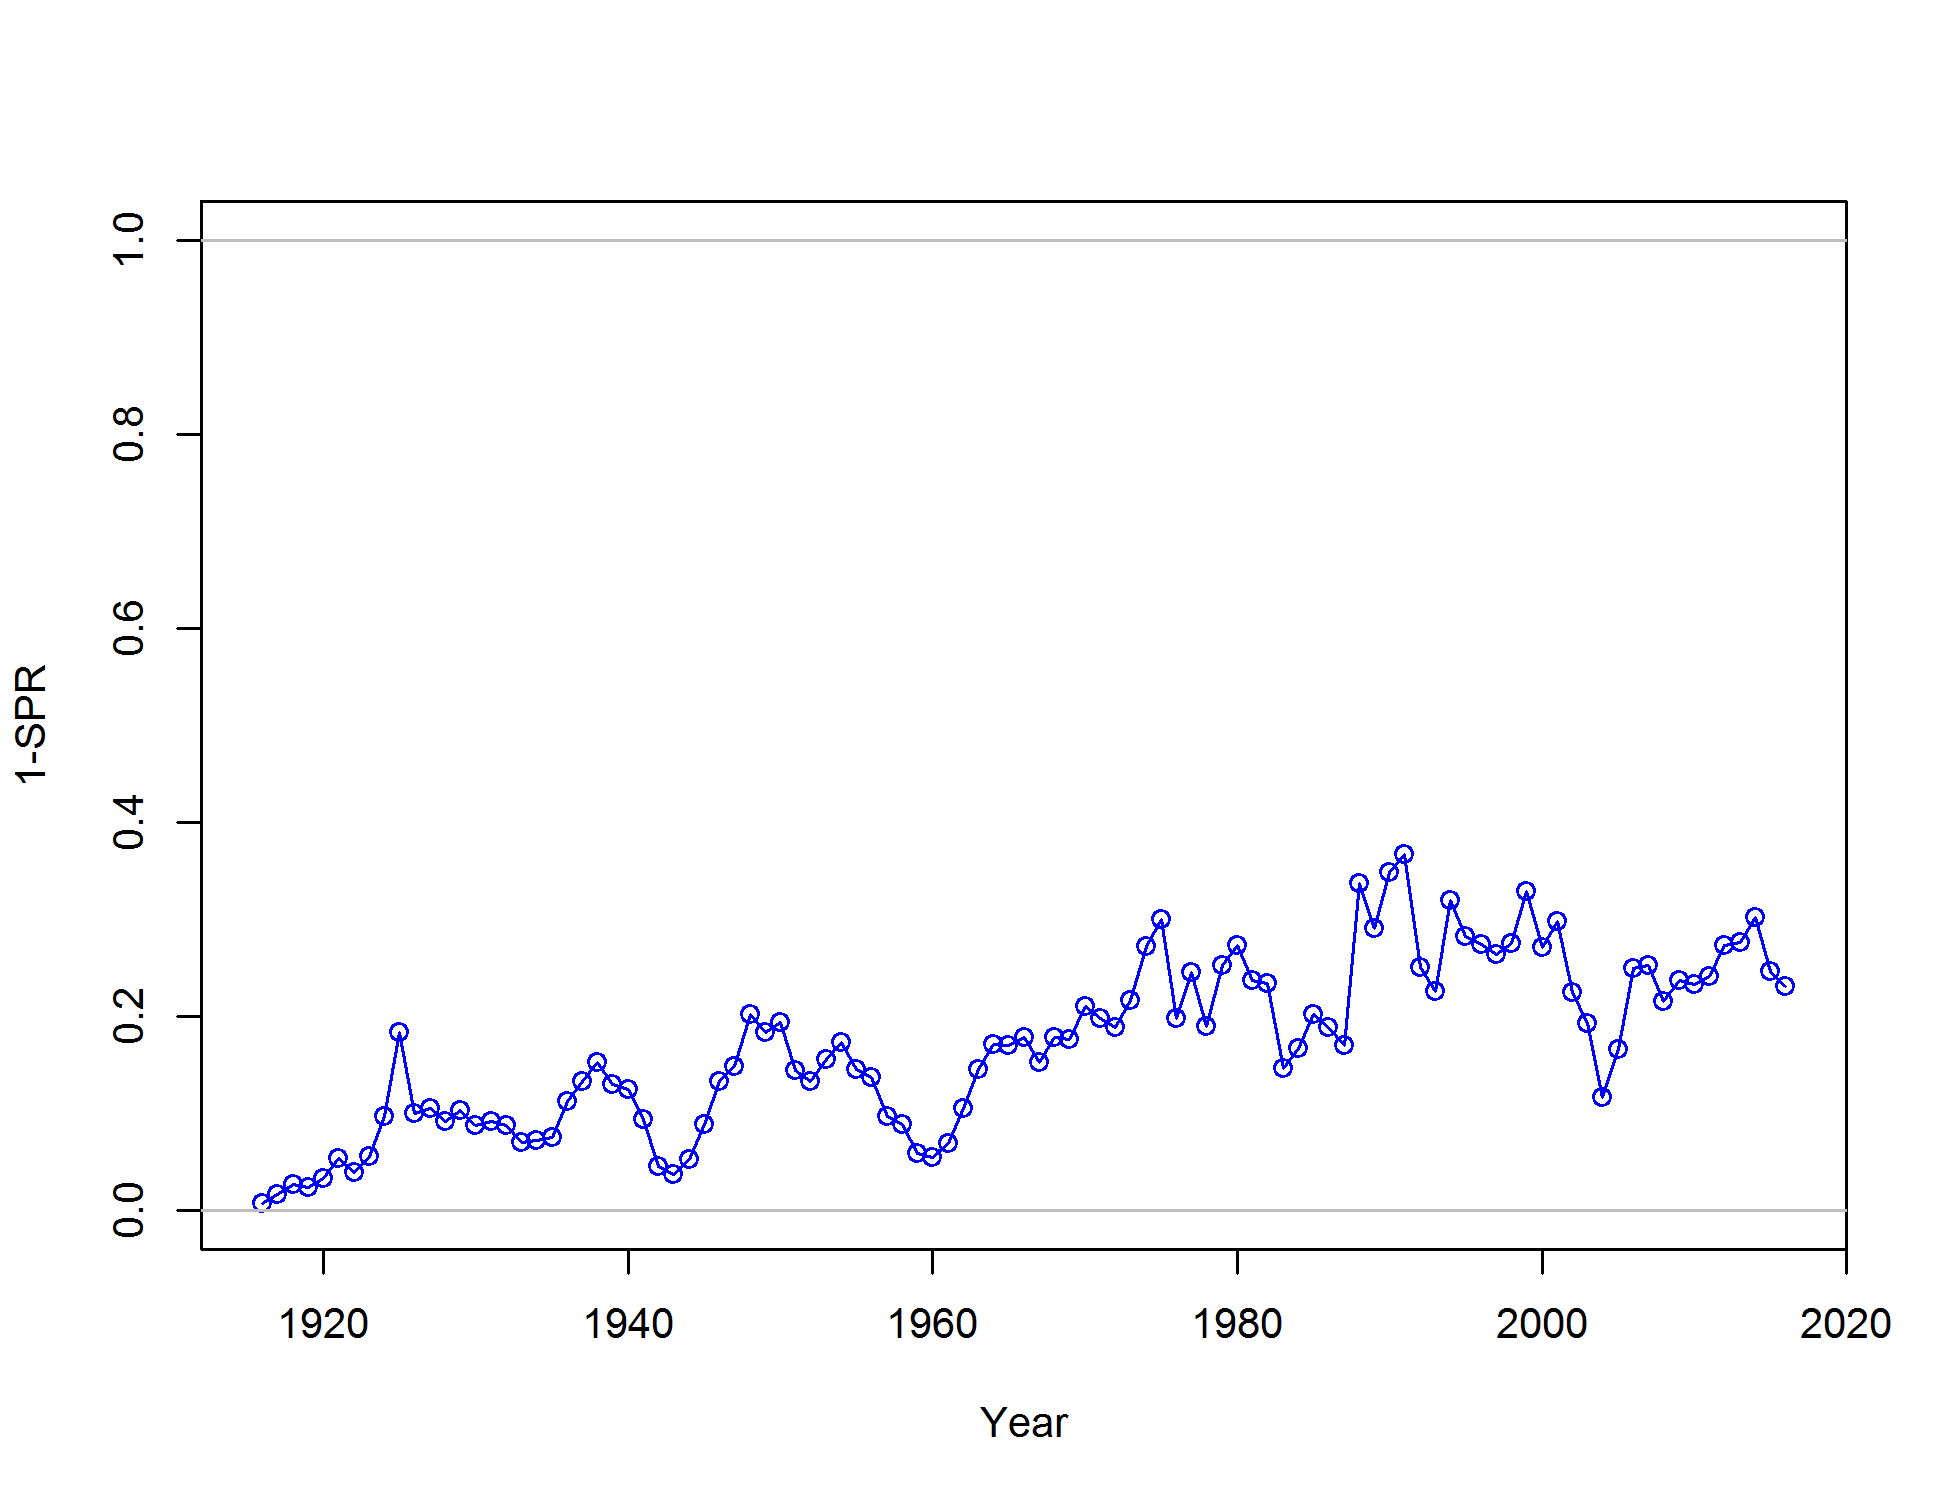
\includegraphics{r4ss/plots_mod1/SPR2_minusSPRseries.png}
\caption{Estimated spawning potential ratio (SPR) for the base-case
model. One minus SPR is plotted so that higher exploitation rates occur
on the upper portion of the y-axis. The management target is plotted as
a red horizontal line and values above this reflect harvests in excess
of the overfishing proxy based on the SPR\textsubscript{50\%} harvest
rate. The last year in the time series is 2016. \label{fig:SPR_all}}
\end{figure}

\FloatBarrier

\subsection*{Ecosystem Considerations}\label{ecosystem-considerations}
\addcontentsline{toc}{subsection}{Ecosystem Considerations}

In this assessment, ecosystem considerations were not explicitly
included in the analysis.\\
This is primarily due to a lack of relevant data and results of analyses
(conducted elsewhere) that could contribute ecosystem-related
quantitative information for the assessment.

\subsection*{Reference Points}\label{reference-points}
\addcontentsline{toc}{subsection}{Reference Points}

This stock assessment estimates that California scorpionfish in the base
model is above the biomass target (\(SB_{40\%}\)), and well above the
minimum stock size threshold (\(SB_{25\%}\)). The estimated relative
depletion level for the base model in 2017 is 54.3\% (95\% asymptotic
interval: \(\pm\) 43\%-65.7\%, corresponding to an unfished spawning
biomass of 882.457 mt (95\% asymptotic interval: 484.21-1280.71 mt) of
spawning biomass in the base model (Table \ref{tab:Ref_pts_mod1}).
Unfished age 1+ biomass was estimated to be 2921.9 mt in the base case
model. The target spawning biomass (\(SB_{40\%}\)) is 649.8 mt, which
corresponds with an equilibrium yield of 247.2 mt. Equilibrium yield at
the proxy \(F_{MSY}\) harvest rate corresponding to \(SPR_{50\%}\) is
232.4 mt (Figure \ref{fig:Yield_all}).

\FloatBarrier

\begin{table}[ht]
\centering
\caption{Summary of reference 
                                      points and management quantities for the 
                                      base case base model.} 
\label{tab:Ref_pts_mod1}
\begin{tabular}{>{\raggedright}p{4.1in}>{\centering}p{.65in}>{\centering}p{1.4in}}
  \hline
\textbf{Quantity} & \textbf{Estimate} & \textbf{\~95\%  Confidence Interval} \\ 
  \hline
Unfished spawning biomass (mt) & 1624.4 & (1156.4-2092.5) \\ 
  Unfished age 1+ biomass (mt) & 2921.9 & (2052.8-3791.1) \\ 
  Unfished recruitment ($R_0$) & 3619.8 & (2518.6-4721) \\ 
  Spawning biomass (2017, mt) & 882.5 & (484.2-1280.7) \\ 
  Depletion (2017) & 0.5432 & (0.4299-0.6565) \\ 
  \textbf{$\text{Reference points based on } \mathbf{SB_{40\%}}$} &  &  \\ 
  Proxy spawning biomass ($B_{40\%}$) & 649.8 & (462.5-837) \\ 
  SPR resulting in $B_{40\%}$ ($SPR_{B40\%}$) & 0.4589 & (0.4589-0.4589) \\ 
  Exploitation rate resulting in $B_{40\%}$ & 0.1741 & (0.1601-0.1882) \\ 
  Yield with $SPR_{B40\%}$ at $B_{40\%}$ (mt) & 247.2 & (168.6-325.9) \\ 
  \textbf{\textit{Reference points based on SPR proxy for MSY}} &  &  \\ 
  Spawning biomass & 723.8 & (515.2-932.3) \\ 
  $SPR_{proxy}$ & 0.5 &  \\ 
  Exploitation rate corresponding to $SPR_{proxy}$ & 0.1502 & (0.1383-0.1621) \\ 
  Yield with $SPR_{proxy}$ at $SB_{SPR}$ (mt) & 232.4 & (158.5-306.4) \\ 
  \textbf{\textit{Reference points based on estimated MSY values}} &  &  \\ 
  Spawning biomass at $MSY$ ($SB_{MSY}$) & 358.8 & (250.6-467) \\ 
  $SPR_{MSY}$ & 0.2974 & (0.2857-0.3091) \\ 
  Exploitation rate at $MSY$ & 0.3236 & (0.2917-0.3554) \\ 
  $MSY$ (mt)  & 281.3 & (192.2-370.4) \\ 
   \hline
\end{tabular}
\end{table}

\FloatBarrier

\subsection*{Management Performance}\label{management-performance}
\addcontentsline{toc}{subsection}{Management Performance}

California scorpionfish has been managed as a single-species outside of
a complex since 2003. The estimated catch of California scorpionfish
north below the ACL in all years (2007-2017) except for in 2014 when the
catch exceeded the ACL (and ABC) by 6.8 mt. A summary of these values as
well as other base case summary results can be found in Table
\ref{tab:mnmgt_perform}.

\begin{table}[ht]
\centering
\caption{Recent trend in total catch (mt) relative to the 
                              harvest specifications. Estimated total catch reflect 
                              the commercial and recreational removals.  The OFL 
                                was termed the ABC prior to implementation of the FMP 
                                Amendment 23 in 2011.  Likewise, the ACL was termed 
                                OY prior to 2011 and the ABC was redefined to reflect 
                                the uncertainty in estimating the OFL.} 
\label{tab:mnmgt_perform}
\scalebox{0.9}{
\begin{tabular}{>{\raggedleft}p{1in}>{\centering}p{1in}>{\centering}p{1in}>{\centering}p{1in}>{\centering}p{1in}>{\centering}p{1in}}
  \hline
Year & OFL (mt; ABC prior to 2011) & ABC (mt) & ACL (mt; OY prior to 2011) & ACT & Estimated total catch (mt) \\ 
  \hline
\textbf{2007} & 219 &  & 175 &  & 139.583 \\ 
  \textbf{2008} & 219 &  & 175 &  & 103.887 \\ 
  \textbf{2009} & 175 &  & 175 &  & 113.318 \\ 
  \textbf{2010} & 155 &  & 155 &  & 105.968 \\ 
  \textbf{2011} & 141 & 135 & 135 &  & 105.215 \\ 
  \textbf{2012} & 132 & 126 & 126 &  & 120.008 \\ 
  \textbf{2013} & 126 & 120 & 120 &  & 115.142 \\ 
  \textbf{2014} & 122 & 117 & 117 &  & 123.822 \\ 
  \textbf{2015} & 119 & 114 & 114 &  & 83.8908 \\ 
  \textbf{2016} & 117 & 111 & 111 &  & 74.1613 \\ 
  \textbf{2017} & 289 & 264 & 150 & 110 & - \\ 
  \textbf{2018} & 278 & 254 & 150 & 110 & - \\ 
   \hline
\end{tabular}
}
\end{table}

\subsection*{Unresolved Problems and Major
Uncertainties}\label{unresolved-problems-and-major-uncertainties}
\addcontentsline{toc}{subsection}{Unresolved Problems and Major
Uncertainties}

As in most/all stock assessments, the appropriate value for
stock-recruit steepness remains a major uncertainty for California
scorpionfish. In this assessment a prior value from a meta-analysis of
West Coast rockfish was used.

Assessment results for the base model are sensitive to natural
mortality. When the natural mortality parameter is estimated by the
model, the result is a value of female natural mortality that is higher
than the STAT believed is biologically plausible. At the high value of
female natural mortality also produced a stock with an estimated
\(lnR_0\) an order of magnitude higher than when natural mortality was
fixed at the prior. Additional analyses and studies should be conducted
to determine an appropriate prior distribution for California
scorpionfish.

The time series of recruitment deviations is driving the trend in
abundance in the base model. Initial explorations of mapping the
estimated recruitment deviations to the CalCOFI sea surface temperature
indicated correlations may be present. Additional research should be
conducted to explore the environmental drivers related to California
scorpionfish recruitment.

The NMFS shelf-slope survey was the only available source of otoliths
for California scorpionfish. It it unknown if the age and length
distribution of the California scorpionfish deeper than 55 m (survey
area) is the similar to that in waters shallower than 55 m. The majority
of California scorpionfish aged were males, and it is unknown if that
was driven by the depth distribution, time of sampling, or other
factors.

The current term of reference for stock assessment require development
of a single decision table with states of nature ranging along the
dominant axis of uncertainty. This presumes that uncertainty is
consequential only for a single variable or estimated quantity, such as
natural mortality, steepness, or ending biomass. This approach may fail
to capture important elements of uncertainty that should be communicated
to the Council and its advisory bodies. Additional flexibility in the
development of decision tables is needed.

\FloatBarrier

\subsection*{Decision Table}\label{decision-table}
\addcontentsline{toc}{subsection}{Decision Table}

The forecasts of stock abundance and yield were developed using the
final base model, with the forecasted projections of the OFL presented
in Table \ref{tab:OFL_projection}. The total catches in 2017 and 2018
are set to the PFMC adopted California scorpionfish ACL of 150 mt.

Uncertainty in the forecasts is based upon the three states of nature
agreed upon at the STAR panel and are based on a low value of \(M\),
0.164, the base model value of \(M\), 0.235, and a high value, 0.2745.
The decision table based sigma was larger than the value for a category
one species of 0.36. Therfore, the sigma was estimated as 0.582 from
\((ln(BaseSpawnOut2017) - ln(LowSpawnOut2017))/1.15\). The resulting
buffer, given a \(p^* = 0.45\), was 0.929. The total catches in 2017 and
2018 are set to the average annual catch from 2015-2016 (79.03) and not
the ABC or OFL due recent trends in total catch being significantly
lower than the OFL and ABC. The average of 2015-2016 catch by fleet was
used to distribute catches in forecasted years. Current medium-term
forecasts based on the alternative states of nature project that the
stock, under the current control rule as applied to the base model, will
decline towards the target stock size Table
\ref{tab:Decision_table_mod1}. The current control rule under the low
state of nature results in a stock decline into the precautionary zone,
while the high state of nature maintains the stock at nearer unfished
levels. Removing the high \(M\) catches under the base model \(M\) and
high \(M\) states of nature results in the population going remaining at
a level of spawning biomass during the projection period, and higher
initial values of \(lnR_0\).

\begin{table}[ht]
\centering
\caption{Projections of potential OFL (mt) using the base model 
                                        forecast and assuming a total catch of 150 mt in 2017 and 2018. 
                                        The control rule target is set to 0.956.} 
\label{tab:OFL_projection}
\begin{tabular}{rr}
  \hline
Year & OFL \\ 
  \hline
2017 & 274.71 \\ 
  2018 & 297.86 \\ 
  2019 & 336.59 \\ 
  2020 & 332.51 \\ 
  2021 & 317.30 \\ 
  2022 & 300.78 \\ 
  2023 & 286.95 \\ 
  2024 & 276.30 \\ 
  2025 & 268.27 \\ 
  2026 & 262.21 \\ 
  2027 & 257.60 \\ 
  2028 & 254.09 \\ 
   \hline
\end{tabular}
\end{table}\begin{table}[ht]
\centering
\caption{Summary of 10-year 
                                             projections beginning in 2018 
                                             for alternate states of nature based on 
                                             an axis of uncertainty for the base model.  Columns range over low, mid, and high
                                             states of nature, and rows range over different 
                                             assumptions of catch levels. An entry of "--" 
                                             indicates that the stock is driven to very low 
                                             abundance under the particular scenario.} 
\label{tab:Decision_table_mod1}
\scalebox{0.85}{
\begin{tabular}{l|cc|>{\centering}p{.7in}c|>{\centering}p{.7in}c|>{\centering}p{.7in}c}
   \multicolumn{3}{c}{}  &  \multicolumn{2}{c}{} 
                               & \multicolumn{2}{c}{\textbf{States of nature}} 
                               & \multicolumn{2}{c}{} \\
  \multicolumn{3}{c}{}  &  \multicolumn{2}{c}{Low M 0.164} 
                               & \multicolumn{2}{c}{Base M 0.235} 
                               &  \multicolumn{2}{c}{High M 0.2745} \\
 \hline
 & Year & Catch & Spawning biomass & Depletion & Spawning biomass & Depletion & Spawning biomass & Depletion \\ 
  \hline
 & 2019 & 150.00 & 587.05 & 0.47 & 1154.73 & 0.71 & 2252.89 & 0.84 \\ 
   & 2020 & 150.00 & 584.87 & 0.47 & 1174.89 & 0.72 & 2312.02 & 0.86 \\ 
   & 2021 & 150.00 & 574.64 & 0.46 & 1176.29 & 0.72 & 2331.33 & 0.87 \\ 
  Constant & 2022 & 150.00 & 561.72 & 0.45 & 1169.09 & 0.72 & 2330.83 & 0.87 \\ 
  Catch & 2023 & 150.00 & 548.66 & 0.44 & 1158.79 & 0.71 & 2321.64 & 0.86 \\ 
   & 2024 & 150.00 & 536.43 & 0.43 & 1148.13 & 0.71 & 2309.70 & 0.86 \\ 
   & 2025 & 150.00 & 525.20 & 0.42 & 1138.24 & 0.70 & 2297.82 & 0.86 \\ 
   & 2026 & 150.00 & 514.89 & 0.41 & 1129.45 & 0.70 & 2287.10 & 0.85 \\ 
   & 2027 & 150.00 & 505.35 & 0.40 & 1121.77 & 0.69 & 2277.85 & 0.85 \\ 
   & 2028 & 150.00 & 496.46 & 0.40 & 1115.12 & 0.69 & 2270.05 & 0.85 \\ 
   \hline
 & 2019 & 232.40 & 587.05 & 0.46 & 1154.73 & 0.71 & 2252.89 & 0.83 \\ 
   & 2020 & 232.40 & 539.94 & 0.43 & 1129.81 & 0.69 & 2267.62 & 0.84 \\ 
   & 2021 & 232.40 & 488.83 & 0.38 & 1091.54 & 0.67 & 2248.79 & 0.83 \\ 
  Estimated & 2022 & 232.40 & 440.88 & 0.35 & 1051.19 & 0.64 & 2217.13 & 0.82 \\ 
  MSY & 2023 & 232.40 & 398.12 & 0.31 & 1013.73 & 0.62 & 2183.03 & 0.81 \\ 
   & 2024 & 232.40 & 360.29 & 0.28 & 980.74 & 0.60 & 2151.29 & 0.80 \\ 
   & 2025 & 232.40 & 325.87 & 0.25 & 952.17 & 0.58 & 2123.53 & 0.79 \\ 
   & 2026 & 232.40 & 293.92 & 0.23 & 927.43 & 0.57 & 2099.95 & 0.78 \\ 
   & 2027 & 232.40 & 263.85 & 0.21 & 905.91 & 0.55 & 2080.12 & 0.77 \\ 
   & 2028 & 232.40 & 235.33 & 0.18 & 887.07 & 0.54 & 2063.54 & 0.76 \\ 
   \hline
 & 2019 & 337.40 & 587.05 & 0.47 & 1154.73 & 0.71 & 2252.89 & 0.84 \\ 
   & 2020 & 326.81 & 484.09 & 0.39 & 1073.09 & 0.66 & 2211.40 & 0.82 \\ 
   & 2021 & 307.52 & 390.83 & 0.31 & 991.72 & 0.61 & 2150.46 & 0.80 \\ 
  ACL = ABC & 2022 & 288.62 & 320.06 & 0.26 & 926.68 & 0.57 & 2095.21 & 0.78 \\ 
   & 2023 & 273.50 & 269.27 & 0.21 & 879.51 & 0.54 & 2052.75 & 0.76 \\ 
   & 2024 & 262.14 & 230.32 & 0.18 & 846.34 & 0.52 & 2022.64 & 0.75 \\ 
   & 2025 & 253.68 & 197.08 & 0.16 & 822.85 & 0.51 & 2002.27 & 0.75 \\ 
   & 2026 & 247.35 & 167.13 & 0.13 & 805.86 & 0.50 & 1989.02 & 0.74 \\ 
   & 2027 & 242.56 & 139.73 & 0.11 & 793.31 & 0.49 & 1980.76 & 0.74 \\ 
   & 2028 & 238.90 & 114.30 & 0.09 & 783.94 & 0.48 & 1976.01 & 0.74 \\ 
   \hline
\hline
\end{tabular}
}
\end{table}

\begin{sidewaystable}[ht]
\centering
\caption{Base case results summary.} 
\label{tab:base_summary}
\scalebox{0.6}{
\begin{tabular}{r>{\centering}p{1.1in}>{\centering}p{1.1in}>{\centering}p{1.1in}>{\centering}p{1.1in}>{\centering}p{1.1in}>{\centering}p{1.1in}>{\centering}p{1.1in}>{\centering}p{1.1in}>{\centering}p{1.1in}>{\centering}p{1.1in}}
  \hline
Quantity & 2008 & 2009 & 2010 & 2011 & 2012 & 2013 & 2014 & 2015 & 2016 & 2017 \\ 
  \hline
Landings (mt) &  &  &  &  &  &  &  &  &  &  \\ 
  Total Est. Catch (mt) &  &  &  &  &  &  &  &  &  &  \\ 
  OFL (mt) &  &  &  &  &  &  &  &  &  &  \\ 
  ACL (mt) &  &  &  &  &  &  &  &  &  &  \\ 
   \hline
(1-$SPR$)(1-$SPR_{50\%}$) & 0.43 & 0.47 & 0.47 & 0.49 & 0.55 & 0.56 & 0.61 & 0.50 & 0.47 &  \\ 
   \hline
Exploitation rate & 0.05 & 0.06 & 0.05 & 0.06 & 0.07 & 0.07 & 0.08 & 0.05 & 0.04 &  \\ 
  Age 1+ biomass (mt) & 2306.33 & 2156.96 & 2047.95 & 1948.44 & 1869.84 & 1768.52 & 1630.70 & 1556.37 & 1534.81 & 1713.25 \\ 
   \hline
Spawning biomass & 1144.500 & 1090.480 & 1029.330 &  980.130 &  943.555 &  890.084 &  810.223 &  746.227 &  774.813 &  882.457 \\ 
  ~95\% CI & (654.46-1634.54) & (629.78-1551.18) & (597.2-1461.46) & (571.79-1388.47) & (553.81-1333.3) & (518.85-1261.32) & (462.86-1157.59) & (412.08-1080.38) & (426.28-1123.35) & (484.21-1280.71) \\ 
   \hline
Depletion & 0.705 & 0.671 & 0.634 & 0.603 & 0.581 & 0.548 & 0.499 & 0.459 & 0.477 & 0.543 \\ 
  ~95\% CI & (0.573-0.836) & (0.55-0.793) & (0.521-0.746) & (0.5-0.707) & (0.485-0.677) & (0.456-0.64) & (0.41-0.587) & (0.371-0.548) & (0.381-0.572) & (0.43-0.657) \\ 
   \hline
Recruits & 2288.15 & 2589.07 & 2483.75 & 1178.81 & 1112.10 & 3747.47 & 3529.05 & 7585.54 & 3268.02 & 3343.81 \\ 
  ~95\% CI & (1198.27 - 4369.33) & (1388.65 - 4827.18) & (1330.55 - 4636.43) & (541.36 - 2566.83) & (509.72 - 2426.35) & (2048.29 - 6856.23) & (1626.81 - 7655.6) & (3389.96 - 16973.8) & (1063.03 - 10046.74) & (1088.44 - 10272.52) \\ 
   \hline
\end{tabular}
}
\end{sidewaystable}

\begin{figure}[htbp]
\centering
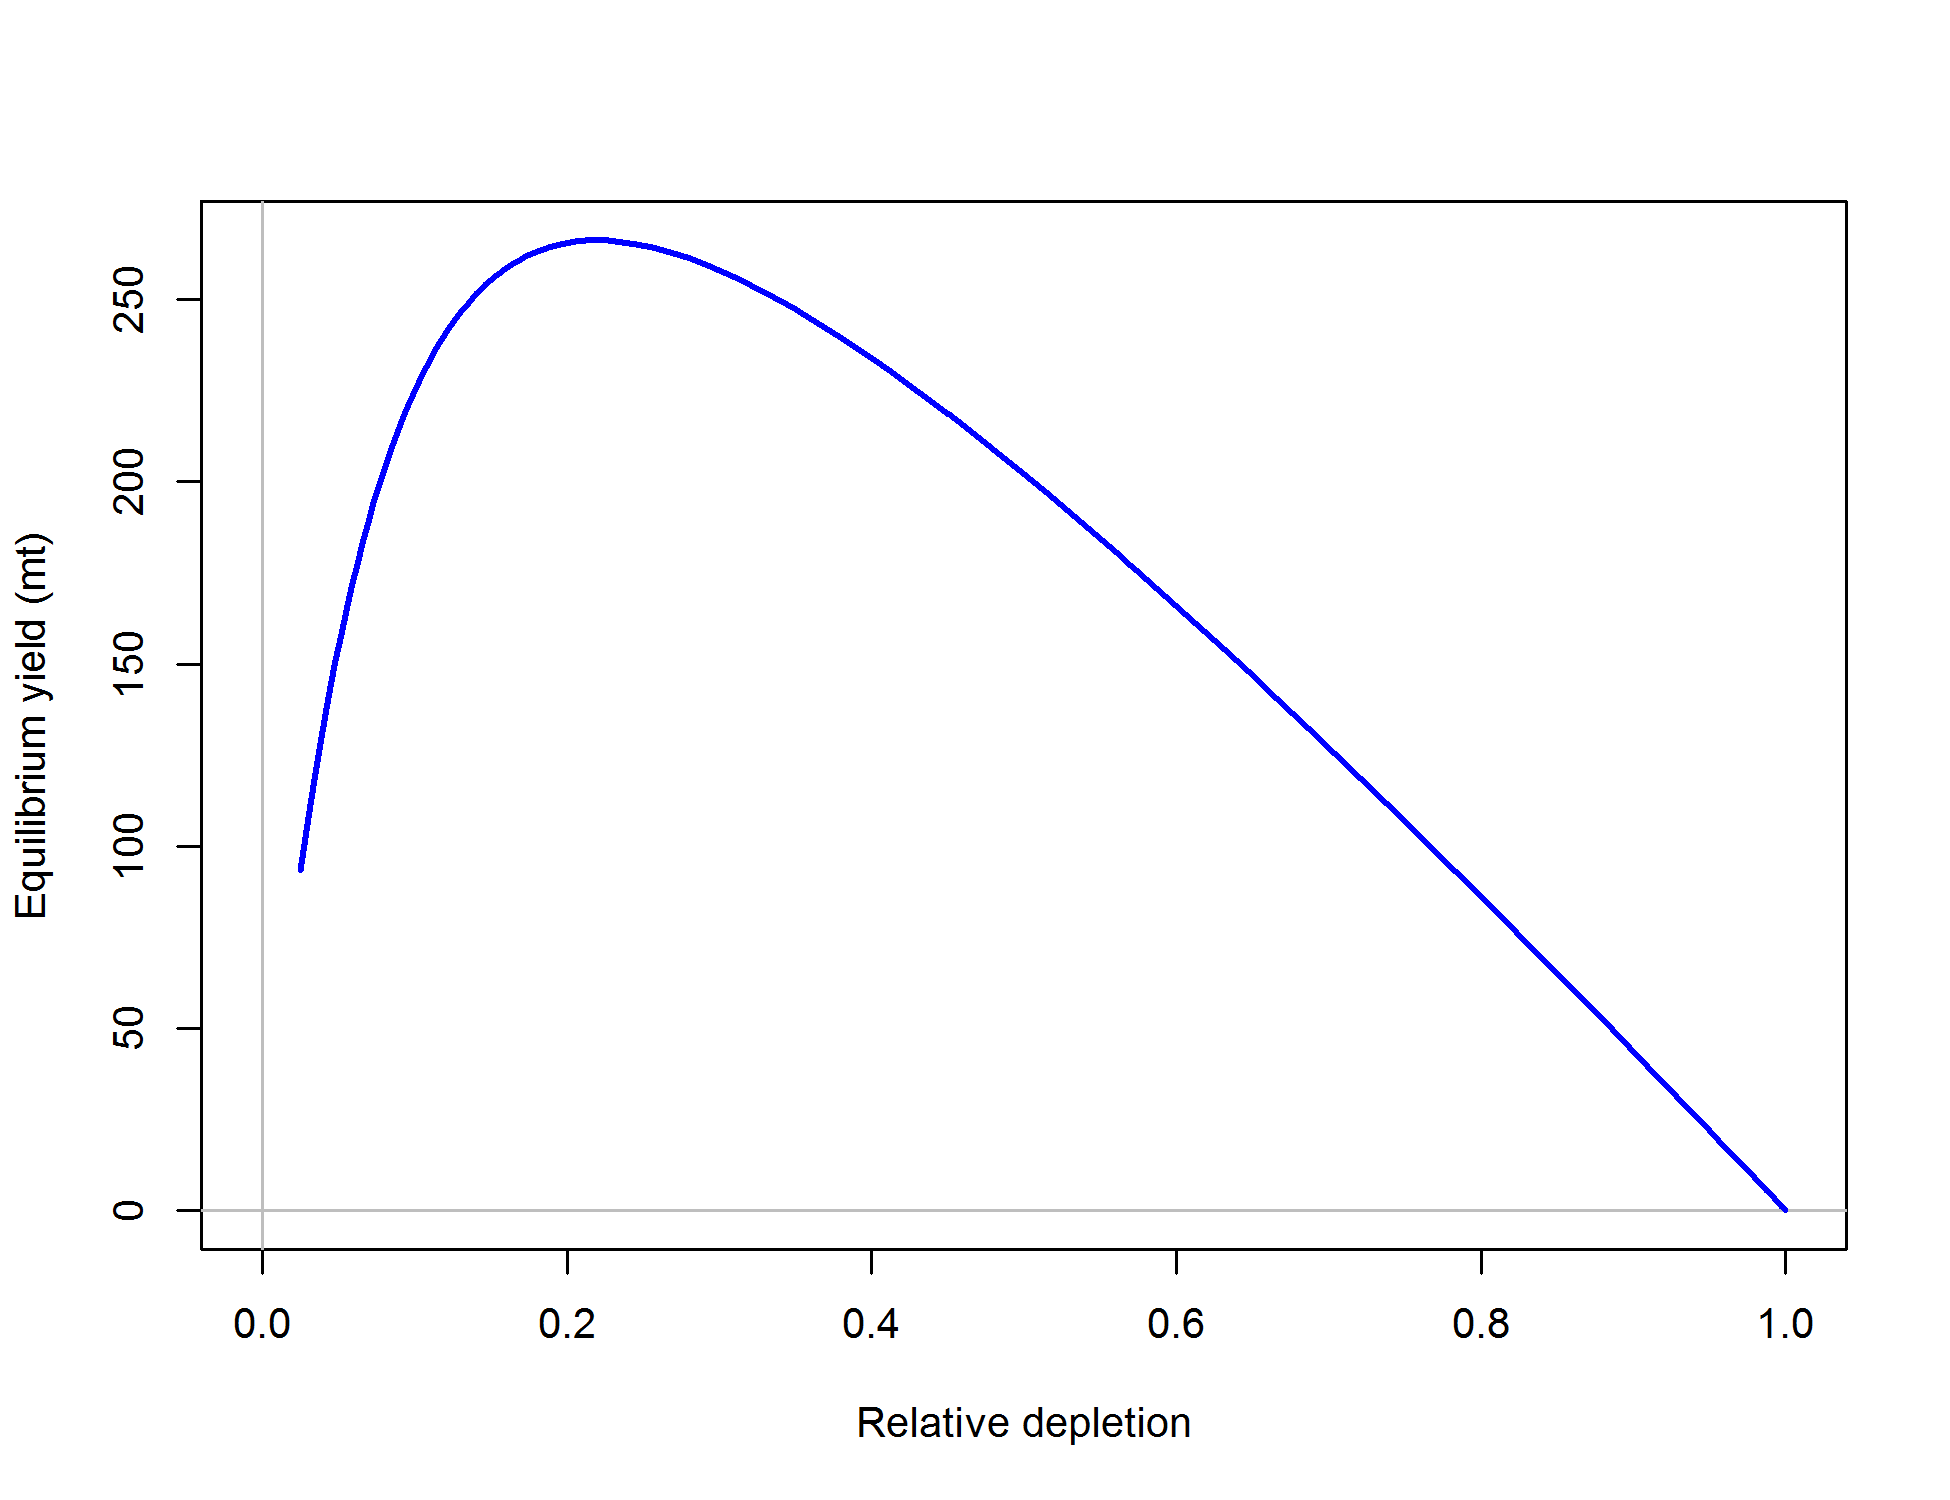
\includegraphics{r4ss/plots_mod1/yield1_yield_curve.png}
\caption{Equilibrium yield curve for the base case model. Values are
based on the 2016 fishery selectivity and with steepness fixed at 0.718.
\label{fig:Yield_all}}
\end{figure}

\FloatBarrier

\newpage

\subsection*{Research and Data Needs}\label{research-and-data-needs}
\addcontentsline{toc}{subsection}{Research and Data Needs}

We recommend the following research be conducted before the next
assessment:

There are a number of areas of research that could improve the stock
assessment for California scorpionfish. Below are issues identified by
the STAT team and the STAR panel:

\begin{enumerate}

\item \textbf{Natural mortality}: Both natural mortality and steepness were 
fixed in the base model.  The natural mortality estimate used the assessment 
was based on maximum age. The collection of age data for older females may improve 
the ability to estimate female natural mortality in the model.  The NWFSC trawl survey
was the only available source of age data for this assessment, of which there were a 
number of age-1 fish and the data were dominated by males.  It may also be possible 
to evaluate mortality by quantifying predation by major predators of scorpionfish, 
such as octopus. 

Tagging study to estimate natural mortality for scorpionfish should be 
considered.  This project could be designed as a cooperative research project 
with the charter fleet in southern California.

\item \textbf{Steepness}: California scorpionfish has not been fished to a level 
where information on steepness is available.  A meta-analysis of steepness should be done for 
species with the same reproductive strategy as scorpionfish.


\item \textbf{Stock south of the U.S. border}:  No available information on the status of California 
scorpionfish in Mexico could be found.  A number of emails were sent to researchers 
in Mexico and none were returned.  It is known that a portion of the stock resides 
in Mexico and that boat leaving from San Diego target California scorpionfish off 
the Coronado Islands.  

\item \textbf{Sex ratio}:  The sex ratio in the only published work by Love et al.
(\protect\hyperlink{ref-Love1987}{1987}) and samples 
from the NWFSC trawl survey were skewed towards males. Data on sex ratios from the 
recreational or commercial fisheries would help in determining the sex ratio of the population.


\item \textbf{Aggregating behavior}: Aggregative behavior in both spawning and 
non-spawning seasons of California scorpionfish is not well understood. Studies are 
needed to evaluate the environmental or ecological conditions that govern this behavior.



\item \textbf{Fecundity/maturity}: A reproductive biology study of California 
scorpionfish is needed.There are currently no estimates of fecundity 
for California scorpionfish.  The hard copies of data from the only
estimates of maturity for California scorpionfish by Love et al. 
(\protect\hyperlink{ref-Love1987}{1987}) are no longer available.  
Some data on the spatial distribution of the 
eggs are available from CalCOFI, but were not keypunched to the species level. 
California scorpionfish mature at a young age, and additional data can help 
inform the maturity ogive.

No studies have been done of the relationship between weight and reproductive 
output.  California scorpionfish have a different reproductive strategy than rockfish, 
and seasonal protection of spawning areas may help maintain reproductive capacity 
of the stock.

\item \textbf{Discard mortality}: Many scorpionfish are discarded at sea. The assessment 
used estimates of discard mortality of a distantly related species (lingcod) 
in a different ecological setting (Karpov \protect\hyperlink{ref-Karpov1996}{1996}). 
Studies of discard mortality are needed 
to parametrize the assessment model.

\item \textbf{Environmental covariates}: The relationship between environmental 
conditions and recruitment for scorpionfish should be further explored. Preliminary 
exploration using CalCOFI temperature data suggested that a relationship existed, 
but other time series may correlate more strongly given that scorpionfish are a 
near-shore species.  Scorpionfish appear to be a relatively hardy and adaptable 
species and may expand northward in a warming climate.  


\item \textbf{Stephens and MacCall filtering}: Ad hoc criteria are used to identify 
a threshold when applying the Stephens and MacCall method of selecting records for 
CPUE index development.  Further research is needed to determine whether threshold 
selection criteria can be optimized.


\item \textbf{Discard fleet modeling}: Modeling discard as a separate fleet, as 
was done for California scorpionfish, is a simple and intuitive approach, but 
the strengths and weaknesses of this approach are unclear. This method should 
be compared to the more standard approach of modeling discard with retention 
curves to ensure the model results are not strongly affected by the method used.


\item \textbf{MCMC in Stock Synthesis}: The Markov chain Monte Carlo (MCMC) 
method implemented in Stock Synthesis is not reliable in many cases.  
Characterizing uncertainty of the final assessment model is important, and 
MCMC offers advantages over asymptotic approximations using the Hessian or 
likelihood profiles. 

\item \textbf{Decision tables}: Several alternative approaches were used this 
year to construct decision tables and some approaches may be better than others. 
The stock assessment TOR should outline the various methods that can be used, 
and provide recommendations if possible on preferred approaches.


\item \textbf{POTW trawl surveys}: Additional biological information 
(sex, otoliths, depth distribution) should be collected for California 
scorpionfish during the Publicly Owned Treatment Works (POTWs) trawl 
survey and the Southern California Bight Regional Monitoring Project 
(SCCWRP) trawl survey.

\item \textbf{Age validation}: An age validation study is needed for 
California scorpionfish.


\item \textbf{CalCOFI}: CalCOFI ichthyoplankton surveys in southern California 
do not currently identify scorpionfish eggs to species, though it is possible to 
do this in southern California waters. Species-specific identification of 
scorpionfish eggs is recommended to develop spawning output index for use in 
the next stock assessment.



\end{enumerate}

\FloatBarrier

\newpage

\renewcommand{\thefigure}{\arabic{figure}}
\renewcommand{\thetable}{\arabic{table}}

\setcounter{figure}{0} \setcounter{table}{0}

\pagenumbering{arabic}

\section{Introduction}\label{introduction}

\subsection{Basic Information and Life
History}\label{basic-information-and-life-history}

California scorpionfish (\emph{Scorpaena guttata}), also known as
sculpin, originates from the Greek word for scorpionfishes and
\emph{guttata} is Latin for speckled. California scorpionfish is a
medium-bodied fish and like other species in the genus \emph{Scorpaena},
it produces a toxin in its dorsal, anal, and pectoral fin spines, which
produces intense, painful wounds (Love et al.
\protect\hyperlink{ref-Love1987}{1987}). Scorpionfish are very resistant
to hooking mortality and have shown survival under extreme conditions.

Its range extends from central California (Santa Cruz) to the Gulf of
California, although within U.S. waters they are most common in the
Southern California Bight (Eschmeyer et al.
\protect\hyperlink{ref-Eschmeyer1983}{1983}, Love et al.
\protect\hyperlink{ref-Love1987}{1987}). The species generally inhabits
rocky reefs, caves and crevices, but in certain areas and seasons it
aggregates over sandy or muddy substrate (Frey
\protect\hyperlink{ref-Frey1971}{1971}, Love et al.
\protect\hyperlink{ref-Love1987}{1987}). California scorpionfish have
been observed from the intertidal to 600 ft with a preferred depth range
from 20-450 ft. Little is known about the aggregating behaviors of
California scorpionfish. Marine Applied Research and Exploration (MARE)
has observed California scorpionfish aggregations during the spawning
season (June 2014) and also in the late fall (November 2012) from video
transects in southern California. The November spawning aggregation was
observed at a small rocky feature near La Jolla and the June aggregation
was at a sandy area adjacent to the Farnsworth MPAs (Andy Lauermann,
MARE, personal communication).

Males and females show different growth rates, with females growing to a
larger size than males, and the sexes exhibit different length-weight
relationships (Love et al. \protect\hyperlink{ref-Love1987}{1987}). Few
California scorpionfish are mature at one year old (14 cm total length).
Fifty-percent of fish mature at 17-18 cm (2 years old) and all by 22 cm
(4 years old) (Love et al. \protect\hyperlink{ref-Love1987}{1987}).

California scorpionfish feed on a wide variety of mobile prey, including
crabs, fishes (e.g., include northern anchovy, spotted cusk-eel),
octopi, isopods and shrimp, (Taylor
\protect\hyperlink{ref-Taylor1963}{1963}, Quast
\protect\hyperlink{ref-Quast1968}{1968}, Turner et al.
\protect\hyperlink{ref-Turner1969}{1969}, Love et al.
\protect\hyperlink{ref-Love1987}{1987}). The species is nocturnal, but
have been observed feeding during the day. Predation on scorpionfish is
believed to be low, but one individual was found in the gut of a leopard
shark (Milton Love, personal communication, UC Santa Barbara).

\subsection{Early Life History}\label{early-life-history}

California scorpionfish utilize the ``explosive breeding assemblage''
reproductive mode in which fish migrate to, and aggregate at traditional
spawning sites for brief periods (Love et al.
\protect\hyperlink{ref-Love1987}{1987}). California scorpionfish migrate
to deeper waters (120-360 ft) to spawn during May-August, with peak
spawning occurring July. The species is oviparous, producing floating,
gelatinous egg masses in which the eggs are embedded in a single layer
(Orton \protect\hyperlink{ref-Orton1955}{1955}) and it is believed that
spawning takes place just before, and perhaps after dawn, in the water
column (Love et al. \protect\hyperlink{ref-Love1987}{1987}). Love et al.
(\protect\hyperlink{ref-Love1987}{1987}) tagged California scorpionfish
and recaptures suggested individuals return to the same spawning site,
but information is not available on non-spawning season site fidelity.

California scorpionfish have been observed in the California Cooperative
Oceanic Fisheries Investigations (CalCOFI) survey, the zooplankton and
ichthyoplankton survey of the California Current System. The CalCOFI
survey observed 463 California scorpionfish larvae from 1977-2000, with
the majority at station close to Oxnard (east of the Channel Islands)
(Moser et al. \protect\hyperlink{ref-Moser2002}{2002}). Higher densities
of larvae have been observed in the CalCOFI stations throughout Baja,
peaking south of Punta Eugenia from July to September. The hatching
length is reported as 1.9-2.0 mm (Washington et al.
\protect\hyperlink{ref-Washington1984}{1984}) and transformation length
of greater than 1.3 cm (Washington et al.
\protect\hyperlink{ref-Washington1984}{1984}) less than 2.1 cm (Moser
\protect\hyperlink{ref-Moser1996}{1996}).

\subsection{Map}\label{map}

A map showing the scope of the assessment and depicting boundaries for
fisheries or data collection strata is provided in Figure
\ref{fig:boundary_map}.

\subsection{Ecosystem Considerations}\label{ecosystem-considerations-1}

In this assessment, ecosystem considerations were not explicitly
included in the analysis. This is primarily due to a lack of relevant
data and results of analyses (conducted elsewhere) that could contribute
ecosystem-related quantitative information for the assessment.

\subsection{Fishery Information}\label{fishery-information}

The hook-and-line fishery off California developed in the late 19th
century (Love et al. \protect\hyperlink{ref-Love2002}{2002}). The
rockfish trawl fishery was established in the early 1940s, when the
United States became involved in World War II and wartime shortage of
red meat created an increased demand for other sources of protein (Harry
and Morgan \protect\hyperlink{ref-Harry1961}{1961}, Alverson et al.
\protect\hyperlink{ref-Alverson1964}{1964}).

California scorpionfish comprise a minor part of the Californian sport
and commercial fisheries (Love et al.
\protect\hyperlink{ref-Love1987}{1987}). Historically, California
scorpionfish were taken commercially by hook and line and, occasionally,
by round haul nets (Daugherty
\protect\hyperlink{ref-Daugherty1949}{1949}). Scorpionfish were commonly
caught around Santa Catalina Island during the late 19th Century with
gill nets (Jordan \protect\hyperlink{ref-Jordan1887}{1887}). The 1937
Bureau of Commercial Fisheries report noted that California scorpionfish
had been a fairly important commercial species for a long time. The
species was targeted by a few fishermen during the summer months, and
was also taken as a bycatch in the rockfish fisheries. By 1949, the
Bureau of Marine Fisheries reported ``{[}Scorpionfish{]} will even come
to the surface to lights at night'' and were also taken in round haul
nets. At that time, scorpionfish were rarely targeted by fishermen
except by a few specialists.

More recently, commercial bottom longlines have been used to target
spawning aggregations offshore of Long Beach (Love et al.
\protect\hyperlink{ref-Love1987}{1987}). Since the early 1990s, trawl
catch has been a substantial component of the commercial catch.
Commercial landings have fluctuated substantially over time, which
could, in part, be due to changes in targeting and El
\(\text{Ni\~{n}o}\) events (Love et al.
\protect\hyperlink{ref-Love1987}{1987}). A high proportion of the catch
landed in California during the 1960s and 1970s was taken from Mexican
waters. In recent years, most of the catch has come from around the Los
Angeles region. In general, the majority of the commercial catch has
come from the Los Angeles region, except in the 1960s and 1970s when the
majority of the catch came from the San Diego region and Mexican waters.

California scorpionfish are most often taken by boat fishermen, but
fairly large numbers are caught from piers, jettys, and rocky shorelines
in the recreational fishery. The Commercial Passenger Fishing Vessel
(CPFV; also referred to as the recreational party/charter or PC mode)
effort has remained relatively constant over a long period (1959-1998)
(Dotson and Charter \protect\hyperlink{ref-Dotson2003}{2003}). However,
there appears to be a shift in effort towards less utilized species,
such as California scorpionfish, over the past decade (Dotson and
Charter \protect\hyperlink{ref-Dotson2003}{2003}). Especially as catch
limits for rockfish have become more restricted commercial passenger
fishing vessels (CPFV) operators target California scorpionfish spawning
aggregations during spring and summer (Love et al.
\protect\hyperlink{ref-Love1987}{1987}), and also target California
scorpionfish in the winter when other fisheries are closed. California
scorpionfish become a target species for day boats during the spawning
months when spawning aggregations can be located. There are a small
number of boats that specialize in targeting these aggregations. The
spawning aggregations occur in deeper waters, often times outside of the
three nautical mile state jurisdiction. It is also unknown what fraction
of the population aggregates during the spawning season, e.g., all
mature fish.

Aggregate mortality has been far below the Annual Catch Limits (ACL)
established by the 2005 stock assessment. The ACL projections from the
2005 assessment assumed that the entire ACL was being taken each year
and as a result, the ACL for each subsequent year declined despite
under-attainment in reality. In addition, in 2014, recreational catch
was higher than expected. As a result, in 2014, the combined
recreational and commercial catch exceeded the OFL by 2mt (1\%)
resulting from assumption that the ACL had been attained. Subsequently,
action was taken to decrease the recreational season by four months
(September 1 - December 31). A catch only update of the stock was
undertaken in 2015 (Wallace and Budrick
\protect\hyperlink{ref-Wallace2015}{2015}) that imputed the actual catch
values since the last assessment, resulting in significant increase in
the OFL and ACL. Retrospectively, the catch in 2014 was well below the
OFL as well as the ACL that would have been in place had the ACL values
from the actual attainment been in place in 2014. Thus the stock has not
been subject to overfishing since the original assessment or been in an
overfished condition historically and is considered healthy. The season
restriction in the recreational fishery remained in place as a
precautionary measure until the full assessment was completed to better
inform the current status of the stock, catch limits and regulations
given the perspective provided.

\subsection{Summary of Management
History}\label{summary-of-management-history}

Prior to the adoption of the Pacific Coast Groundfish Fishery Management
Plan (FMP) in 1982, California scorpionfish (\emph{Scorpaena guttata})
was managed through a regulatory process that included the California
Department of Fish and Wildlife (CDFW) along with either the California
State Legislature or the Fish and Game Commission (FGC) depending on the
sector (recreation or commercial) and fishery. With implementation of
the Pacific Coast Groundfish FMP, California scorpionfish came under the
management authority of the Pacific Fishery Management Council (PFMC),
being incorporated, along with all genera and species of the family
Scorpaenidae, into a federal rockfish classification and managed as part
of ``Remaining Rockfish'' under the larger heading of ``Other Rockfish''
(PFMC (\protect\hyperlink{ref-PFMC2002}{2002},
\protect\hyperlink{ref-PFMC2004}{2004}), Tables 31-39).

The ABCs provided by the PFMC's Groundfish Management Team (GMT) in the
1980s were based on an analysis of commercial landings from the 1960s
and 1970s. For this analysis, most of the rockfishes were lumped into
one large group. This analysis indicated that the landings for rockfish
in the Monterey-Conception area were at or near ABC levels (Pacific
Fishery Management Council \protect\hyperlink{ref-PFMC1993}{1993}). To
keep landings within these adopted harvest targets, the Pacific Coast
Groundfish FMP provided the Council with a variety of management tools
including area closures, season closures, gear restrictions, and, for
the commercial sector, cumulative limits (generally for two-month
periods). With the implementation of a federal groundfish restricted
access program in 1994, allocations of total catch and cumulative limits
began to be specifically set for open access (including most of
California's commercial fisheries that target California scorpionfish in
Southern California) and limited entry fisheries (Figure
\ref{fig:Com_regs}) (Pacific Fishery Management Council
\protect\hyperlink{ref-PFMC2002}{2002},
\protect\hyperlink{ref-PFMC2004}{2004}). As a result, in the later 1990s
as commercial landings decreased and recreational harvest became a
greater proportion of the available harvest.

Beginning in 1997, California scorpionfish was managed as part of the
\emph{Sebastes} complex-south, Other Rockfish category. \emph{Sebastes}
complex-south included the Eureka, Monterey, and Conception areas while
\emph{Sebastes} complex-north included the Vancouver and Columbia
areas.) The PFMC's rockfish management structure changed significantly
in 2000 with the replacement of the \emph{Sebastes} complex -north and
-south areas with Minor Rockfish North (now covering the Vancouver,
Columbia, and Eureka areas) and Minor Rockfish South (now Monterey and
Conception areas only). The OY for these two groups (which continued to
be calculated as 0.50 of the ABC) was further divided (between north and
south of \(40^\circ 10^\prime\) N. latitude) into nearshore, shelf, and
slope rockfish categories with allocations set for Limited Entry and
Open Access fisheries within each of these three categories (January 4,
2000, 65 FR 221; PFMC (\protect\hyperlink{ref-PFMC2002}{2002}), Tables
54-55). Because of its depth range and southern distribution, California
scorpionfish was included within the Minor Rockfish South, Other
Rockfish ABC and managed under the south of \(40^\circ 10^\prime\) N.
latitude nearshore rockfish OY and trip limits (PFMC
(\protect\hyperlink{ref-PFMC2002}{2002}), Table 29).

Along with the above changes, in 2000 the southern area divided into two
separate management areas at Point Lopez, \(36^\circ 00^\prime\) N.
latitude. This was followed in 2001 with the implementation of the
northern rockfish and lingcod management area between
(\(40^\circ 10^\prime\) N. latitude) and Point Conception
(\(34^\circ 27^\prime\) N. latitude); and the southern rockfish and
lingcod management area between Point Conception and the U.S.- Mexico
border. These were later revised starting in 2004 with the northern
rockfish and lingcod management area redefined as ocean waters from the
Oregon-California border (\(42^\circ 00^\prime\) N. latitude) to
\(40^\circ 10^\prime\) N. latitude, the central rockfish and lingcod
management area defined as ocean waters from \(40^\circ 10^\prime\) N.
latitude to Point Conception, and the southern rockfish and management
area continuing to be defined as ocean waters from Point Conception to
the U.S.-Mexico border.

Cowcod Conservation Areas (CCAs) also were established in 2001 to reduce
fishing effort in areas with high encounter rates of cowcod rockfish
(PFMC (\protect\hyperlink{ref-PFMC2002}{2002}), Table 29). These areas
were closed to all recreational and commercial fishing for groundfish
except for minor nearshore rockfish (including California scorpionfish)
within waters less than 20 fathoms. The California Rockfish Conservation
Area (CRCA) was defined as those ocean waters south
\(40^\circ 10^\prime\) N. latitude to the U.S.-Mexico border with
different depth zones specified for the areas north and south of Pt.
Reyes (\(37^\circ 59.73^\prime\) N. latitude).

During the late 1990s and early 2000s, major changes also occurred in
the way that California managed its nearshore fishery. The Marine Life
Management Act (MLMA), which was passed in 1998 by the California
Legislature and enacted in 1999, required that the FGC adopt an FMP for
nearshore finfish. It also gave authority to the FGC to regulate
commercial and recreational nearshore fisheries through FMPs and
provided broad authority to adopt regulations for the nearshore fishery
during the time prior to adoption of the nearshore finfish FMP. Within
this legislation, the Legislature also included commercial size limits
for nine nearshore species including California scorpionfish (10-inch
minimum size) and a requirement that commercial fishermen landing these
nine nearshore species possess a nearshore permit.

Following adoption of the Nearshore FMP and accompanying regulations by
the FGC in fall of 2002, the FGC adopted regulations in November 2002
which established a set of marine reserves around the Channel Islands in
southern California (which became effective April 2003). The FGC also
adopted a nearshore restricted access program in December 2002 (which
included the establishment of a Deeper Nearshore Permit) to be effective
starting in the 2003 fishing year.

Although the Nearshore FMP provided for the management of the nearshore
rockfish and California scorpionfish, management authority for these
species continued to reside with the Council. Even so, for the 2003 and
subsequent fishery seasons, the State provided recommendations to the
Council specific to the nearshore species that followed the directives
set out in the Nearshore FMP. These recommendations, which the Council
incorporated into the 2003 management specifications, included a
recalculated OY for Minor Rockfish South - Nearshore, division of the
Minor Rockfish South - Nearshore into three groups (shallow nearshore
rockfish; deeper nearshore rockfish; and California scorpionfish), and
specific harvest targets and recreational and commercial allocations for
each of these groups.

Also, since the enactment of the MLMA, the Council and State in a
coordinated effort developed and adopted various management
specifications to keep harvest within the harvest targets, including
seasonal and area closures (e.g.~the CCAs; a closure of Cordell Banks to
specific fishing), depth restrictions, minimum size limits, and bag
limits to regulate the recreational fishery and license and permit
regulations, finfish trap permits, gear restrictions, seasonal and area
closures (e.g.~the RCAs and CCAs; a closure of Cordell Banks to specific
fishing), depth restrictions, trip limits, and minimum size limits to
regulate the commercial fishery.

\subsection{Management Performance}\label{management-performance-1}

California scorpionfish has been managed as a single-species outside of
a complex since 2003. The estimated catch of California scorpionfish
north below the ACL in all years (2007-2017) except for in 2014 when the
catch exceeded the ACL (and ABC) by 6.8 mt. A summary of these values as
well as other base case summary results can be found in Table
\ref{tab:mnmgt_perform}.

\subsection{Fisheries Off Mexico}\label{fisheries-off-mexico}

The California scorpionfish's range extends into to Punta Abreojos, Baja
California Sur, Mexico. The species is also found in the northern Gulf
of California and Guadalupe Island. No formal stock assessments have
been conducted for California scorpionfish in Mexican waters.

\section{Assessment}\label{assessment}

\subsection{Data}\label{data}

Data used in the California scorpionfish assessment are summarized in
Figure \ref{fig:data_plot}. Descriptions of the data sources are in the
following sections.

\subsubsection{Commercial Fishery
Landings}\label{commercial-fishery-landings}

Commercial catches of California scorpionfish (often landed as
``sculpin'') are available back to 1916. Landings from 1916 to 1935 are
presented in CDFG Fish Bulletin No. 49 and Bulletin No. 149 provides
tabulated data from 1916 to 1968. Over 99\% of the commercial catches of
California scorpionfish are from south of Pt. Conception. Whenever
possible, catches from north of Pt. Conception and also caught in Mexico
but landed in the U.S. were excluded from the commercial catch
histories.
\href{http://library.ucsd.edu/ceo/fishcatchtables/fish-catch-download.html}{California
Explores the Ocean (CEO)} provides landings data taken from the CDFG
Fish Bulletins in electronic form, as well as electronic copies of all
CDFG Fish Bulletins.

Statewide annual commercial landings are available for California
scorpionfish from 1916 to 1925, and are assumed to be taken by
hook-and-line. Data by area and month are given in a series of
bulletins, each bulletin usually providing information for a single
year. Data by region and month is available for 1926 to 1986. The Santa
Barbara region includes San Luis Obispo, Santa Barbara and Ventura
counties. Catches from this region were included in the catch history
and comprised less than 10 mt for the period from 1926-1968 (the period
when data at the regional scale are available). Catches from Mexico can
be separated from the total catch starting in 1931, although the CDFG
Bulletins do not report catches originating from Mexican waters
available for all years, e.g., 1932-1934. It is assumed that before 1931
there was no catch taken from Mexican waters landed in California.

The \href{http://128.114.3.187/}{CALCOM} database was queried (March 7,
2017) for commercial landing estimates of California scorpionfish in
California, 1969-2016. Landings were stratified by year, quarter,
live/dead, market category, gear group, port complex, and source of
species composition data (actual port samples, borrowed samples, or
assumed nominal market category). All CALCOM California scorpionfish
landing data are either actual port samples or the nominal California
scorpionfish market category. However, catches in CALCOM do not separate
out catches originating from Mexican waters and landed at U.S. ports.

The Commercial Fisheries Information System (CFIS; maintained by CDFW)
contains California catch in pounds by gear and port for 1969 to 2016.
The CFIS data come from landing receipts or ``fish tickets'' filled out
by the markets or fish buyers as required by the state for all
commercial landings. The fish tickets include the CDFW block in which
the majority of the landings were caught. Landings reported from a block
solely in Mexican waters (blocks \textgreater{}900) were removed from
the catch history. Landings with reported blocks 877-882 with area in
both U.S. and Mexican waters were retained in the catch histories.

The commercial catch is dominated by the hook-and-line fishery (89\% of
total catches). The catch by reported gear types: hook-and-line, fish
pot, trawl, gill net, and other can be found in Table
\ref{tab:CommCatches}. Catch taken by fish pot and other gears is added
to the hook-and-line catch in the stock assessment (30.6 mt total from
fish pot and 93.9 mt total from other gears).

In the assessment, catch for 1916 to 1968 is taken from the CDFG Fish
Bulletins. Catch by gear for 1969 to 2004 is taken from CFIS.

\subsubsection{Commercial Discards}\label{commercial-discards}

Information on commercial discards from the West Coast Groundfish
Observer Program (WCGOP) are available starting in 2004. The commercial
fishery for California scorpionfish has been minimal since the early
2003 (averaging 3.5 mt per year). The available length composition data
from the observed discards is minimal, with 151 fish measured from
2004-2015, and less than half a metric ton. Given the discard mortality
of only 7\%, and the small total catches in the recent years, discards
from the commercial fleet are not considered in the assessment.

\subsubsection{Commercial Fishery Length and Age
Data}\label{commercial-fishery-length-and-age-data}

Biological data from commercial fisheries that caught California
scorpionfish were extracted from CALCOM on March 7, 2017. Samples from
the hook and line fishery were available from 1999 (1 trip) and
2013-2015 (1 trip per year), and for 1999 (1 trip) and 2006 (2 trips)
from the trawl fishery. A total of 87 fish were measured and length
compositions were based on expanded catch-weighted landings. The samples
from 1999 for both fisheries were replaced by samples from the market
category study described below.

The CDFW conducted a market study from 1990-2004 in southern California
(Laughlin and Ugoretz \protect\hyperlink{ref-Laughlin1998}{1998}) to
monitor and summarize local commercial catches. The ports sampled
included San Diego, Santa Barbara/Ventura and Long Beach/San Pedro. Very
few of the samples from Santa Barbara and San Diego (four samples each
from the hook-and-line and trawl fisheries Santa Barbara, and one sample
from the hook-and-line fishery in San Diego) reported California
scorpionfish, and are excluded from the length composition data. Length
composition for California scorpionfish are available from the Long
Beach samples for the hook-and-line (Table
\ref{tab:ComHL_lengthsample}), gillnet (Table
\ref{tab:ComNet_lengthsample}), and trawl fisheries (Table
\ref{tab:ComTrawl_lengthsample}). Length samples from both groundfish
(otter) trawls and single-rigged shrimp trawls were available from the
market study. The average size of fish from the otter trawls (26.5 cm)
was smaller than from the shrimp trawl samples (28.1 cm). Over 70\% of
California scorpionfish catch from the trawl sector was landed from
single-rigged shrimp trawls, which best represent the length composition
of the trawl fleet (CALCOM).

The input sample sizes were calculated via the Stewart Method (Ian
Stewart, personal communication, IPHC):

\begin{centering}

Input effN = $N_{\text{trips}} + 0.138 * N_{\text{fish}}$ if $N_{\text{fish}}/N_{\text{trips}}$ is $<$ 44

Input effN = $7.06 * N_{\text{trips}}$ if $N_{\text{fish}}/N_{\text{trips}}$ is $\geq$ 44

\end{centering}

\subsubsection{Sport Fishery Removals and
Discards}\label{sport-fishery-removals-and-discards}

Data used in reconstructing the retained catch and discarded mortality
for California scorpionfish in the California recreational fishery are
from the Commercial Passenger Fishing Vessel (CPFV), i.e., charter or
for-hire boats, logbooks (1932-2017), the Marine Recreational Fishery
Statistical Survey (MRFSS, 1980-2003) and the California Recreational
Fishery Survey (CRFS, 2004-2017). Total catch was accounted for
including retained catch as well as the estimate of fish discarded dead
assuming a 7\% discard mortality rate approved for use in management in
the regulatory specifications for 2009-2010 (Pacific Fishery Management
Council \protect\hyperlink{ref-PFMC2008}{2008}). The MRFSS and CRFS data
provide estimates of mortality for four recreational fishing modes:
party/charter boats, private/rental boats, fishing from man-made
structures,e.g., piers and jetties, and fishing from the beach or banks.

The Coastal County Household Telephone Survey was used to estimate
fishing effort for the MRFSS survey from 1980-2003 and was subject to
potential positive avidity bias in participation by those contacted by
the survey. The party/charter phone survey was used to estimate effort
for CRFS between 2004 and 2010. The phone survey participation rates
were low in the area south of Pt. Conception, introducing a negative
bias in the effort estimates.

Estimates of mortality from the party/charter sector were derived from
the CPFV logbook data from 1932-2010 and CRFS from 2011-2017. Estimated
mortality from the logbook data is consistent with the catch-based
update conducted in 2015 as well as the 2005 stock assessment.

An under-reporting adjustment (assuming an 80\% reporting rate) was
applied to the logbook data, which is the same as in the 2005 stock
assessment was confirmed as the approximate level of reporting in
conversation with the CRFS program director (Connie Ryan, personal
communication, CDFW). The logbook catch was inflated by 20\% from 1936
to 2010. Annual average weights for the party/charter boat retained
catch were derived from the MRFSS or CRFS estimates for 1980-2010 and
the average weight from 1980-1984 was applied to preceding years.

To estimate discard mortality for the party/charter mode, the annual
average weight was applied from lengths collected sampling onboard
CPFVs; CRFS survey from 2004-2010. The annual average weight from was
applied to discards reported in CPFV logbooks from 2004-2010 and the
overall and the average weight was applied to discards from 1995-2003.
For the period between 1980 and 1994, the MRFSS estimates for discards
were used to reflect discarding due to the paucity of data on the number
of discards from party/charter logbooks prior to 1995.

For all other modes, the MRFSS (1980-2003) and CRFS (2004-2017) based
estimates of retained catch and discard mortality were used. There was a
lapse in MRFSS sampling from 1990 through 1992, for which retained catch
and discard mortality were estimated using the average of values three
years before and three years after the lapse for all modes other than
the party/charter mode. For the party/charter mode, estimates of numbers
of fish were available from logbook data and average weight from the
three years before and after this period were applied to provide
estimates for the party/charter mode.

Estimates of retained catch and discards were not available from the
non-party/charter modes prior to 1980, thus the ratio of catch in the
party/charter mode to the other modes for 1980 through 1985 was used to
provide an estimate of catch in the other modes in the years 1932-1979.
In the case of the private/rental mode, a linear ramp in the ratio
adjustment between party/charter and private/rental modes was applied
between 1966 and 1979 from 0.55 in 1980 to 0.10 in 1965, reflecting the
increase in the relative proportion of catch contributed by the
private/rental mode with time as more individuals anglers purchased
vessels, as recommended in the California Catch Reconstruction (Ralston
et al. \protect\hyperlink{ref-Ralston2010}{2010}), and the ratio of 0.10
was assumed for all years prior. The ratio of party/charter estimates to
the man-made structure (MM) and beach/bank (BB) modes was assumed
constant and the average between 1980 and 1989 was applied from 1932 to
1979. Catch estimates from CPFV logbooks were not available during the
World War II era from 1941 until 1946 and catch was assumed to be zero
for all modes during this period. Estimates for retained catch and
discarded mortality for 1928 to 3528 were estimated using a linear ramp
from the value for 1936 to zero in 1928 for the party/charter mode and
ratios party/charter compared to other modes were used to proxy
estimates for other modes based on the resulting ramped values for the
party/charter mode. The final time series of landings and discard
mortality are in Table \ref{tab:Rec_removal}.

Biological samples from the recreational fleets are described in the
sections below.

\subsubsection{Fishery-Dependent Indices of
Abundance}\label{fishery-dependent-indices-of-abundance}

\textbf{CRFS Private Boat Dockside Intercept Survey}

The CDFW provided the CRFS private boat dockside sampling fisheries data
from 2004 to 2016. The data went through several data quality checks to
identify the best subset of available data that are consistent over the
time series and provide a representative relative index of abundance
once standardized. The dockside sampling of the private/rental mode
consists of samples from a primary series of ports (PR1) where the
majority of fishing effort for this mode originates and a secondary
series of ports with historically low effort (PR2). Only PR1 samples
were used for this index as the sampling forms for the PR2 index have
changed over time and the data could not reliably be collapsed to the
trip level. The dockside data consist of two types of data; Type 2 data
contain records of angler-reported catch, i.e., catch that was not
observed by the sampler and Type 3 data includes sampler-examined
retained catch. Of the Type 2 reported catch for scorpionfish, less than
one percent were reported ``thrown back dead'' and five percent reported
as retained to eat. Given that the reported retained catch is a small
fraction of the catch overall and discard mortality of California
scorpionfish is low, only the Type 3 examined catch are used in the
index.

The survey records the number of contributing anglers (number of anglers
on the vessel for the private mode), but does not contain data on hours
fished. For this index, angler-day was the assumed effort. The data were
filtered to trips fishing with hook-and-line gear in southern
California. Trips with a primary fishing area of Mexico were also
removed. The CRFS dockside private boat records with these broad filters
include 44,128 trips of which 3,802 caught California scorpionfish
(8.6\%).

The Stephens-MacCall approach was used to identify trips with a high
probability of catching California scorpionfish (Stephens and MacCall
\protect\hyperlink{ref-Stephens2004}{2004}). Prior to using the
Stephens-MacCall approach to select relevant trips a number of other
filters were applied to the data. Over the course of the time series
only 45 trips from Santa Barbara county encountered California
scorpionfish, ranging from 0-10 trips a year. The Stephens-MacCall
approach was applied with and without trips from Santa Barbara and the
same species were identified as indicators and counter-indicators. For
the final model prior to Stephens-MacCall, trips from Santa Barbara were
excluded, leaving 41,235 trips, and 3,747 of those caught California
scorpionfish (Table \ref{tab:Fleet4_RecPR_dockside_filter}).

Coefficients from the Stephens-MacCall analysis (a binomial GLM) are
positive for species which co-occur with California scorpionfish, and
negative for species that are not caught with California scorpionfish
(Figure \ref{fig:Fleet4_RecPR_dockside_SM}). Potentially informative
species for the Stephens-MacCall analysis were limited to species caught
in at least one percent of all trips and caught in at least five years.
Some of these never occurred with California scorpionfish (strong
`counter-indicators') and records with these species were removed from
the data prior to estimation of the index. Strong counter-indicators for
the CRFS private boat index included yellowfin tuna and dolphinfish.

A total of 8,590 trips were retained following the Stephens-MacCall
filter, with 3,056 all positive California scorpionfish trips retained.
The California scorpionfish recreational fishery in the southern
management area was closed for eight months in 2004 and nine months in
2005. The majority of records from 2004 and 2005 are from the period
when the fishery was closed and were removed from the analysis (Figure
\ref{fig:recregs}). Records from months when the fishery was closed from
2006-2016 were also excluded from the index since this index relies on
sampler-examined retained catch.

Catch per unit effort was modeled using a delta-GLM approach, where the
catch occurrence (binomial) component was modeled using a logit link
function and the positive catch component was modeled after
log-transformation of the response variable, according to a normal
distribution with an identity link function. The units for CPUE are fish
landed/anglers. A gamma distribution for the positive catch component
was also explored, but model selection favored the lognormal model. The
raw CPUE of factors considered in the model by year are shown in Figure
\ref{fig:Fleet4_RecPR_dockside_lograwCPUE}.

Model selection procedures selected the covariates \emph{2-month wave}
and \emph{county} as important for both the catch occurrence and
positive catch component models for all data sets, along with the
categorical year factor used for the index of abundance (Table
\ref{tab:Fleet4_RecPR_dockside_aic}). The Q-Q goodness of fit plot for
the lognormal portion of the model shows a moderate fit to the data
(Figure \ref{fig:Fleet4_RecPR_dockside_QQ}). The final index indicates a
decrease in relative abundance from 2006 to 2010, at which point the
index is relatively flat (Figure \ref{fig:index4_logcpuedata_RecPR} and
Table \ref{tab:Fleet4_RecPR_dockside_index}).

Biological samples from trips retaining California scorpionfish were
collected during the dockside surveys. Lengths of California
scorpionfish from 1980-2016 for the private mode were provided from the
Recreational Fisheries Information Network (RecFIN) by Edward Hibsch
(PSMFC) on November 29, 2016. Length measurements from the private mode
were provided directly from CDFW for the years 2004-2016 Table
\ref{tab:Fleet4_lengthsample}. The number of trips is the number of
unique ID\_CODEs from RecFIN for 1980-2003. Starting in 2004 with the
CRFS program, the number of unique trips sampled in the private boat
mode was recorded. The recreational private fleet tends to select larger
fish than the recreational party/charter fleet, which is one reason the
private and party/charter fleets were maintained as two separate fleets
in the base model. No length data for discarded fish from the
recreational private mode fleet are available.

\textbf{CRFS CPFV Logbook Index}

CPFV operators have been required to submit written catch logs with
daily trips records of catches to CDFW since 1935. The logbook data from
1936-1979 are available as monthly summaries, which do not contain the
level of detail needed for an index of abundance. CDFW provided the CPFV
logbook data from 1980-2016 (Charlene Calac, CDFW). Logbook data from
1980-2016 contain records for each trip, including the fishing date,
port of landing, vessel name and number, CDFG block area fished (Figure
\ref{fig:boundary_map}), angler effort, number of fish kept and
discarded by species. As of 1994, operators were required to report the
number of fish discarded and lost to seals. Prior to 1994, it is assumed
that all reported fish were retained. Details and additional information
on the historical logbook database can be found in Hill and Schneider
(\protect\hyperlink{ref-Hill1999}{1999}).

The number of anglers on board the vessel and the hours fished are
included in the database for all years. Only retained fish are included
in the index of abundance and the unit of effort is angler hours. A
number of data filters were applied to the data to account for possible
mis-reporting, e.g., trips reporting retained California scorpionfish in
top 1\% of the data (\textgreater{}325 fish). Trips fishing outside of
California scorpionfish habitat (reported as targeting pelagic species)
or trips reporting a block with a minimum depth deeper than 140 m were
also filtered out.

Because California scorpionfish is not a primary target species, boats
with fewer than 10 trips retaining California scorpionfish were removed
from the analysis. Data were also filtered to only include catches
reported from blocks South of Pt. Conception and north of the
U.S.-Mexico border (Figure \ref{fig:boundary_map}). For a block to be
retained for the analysis, at least 100 trips retaining California
scorpionfish and a total of 500 trips must have occured in the block. A
full description of the data filters is in Table
\ref{tab:Fleet5_RecPC_CPFVlogbook_filter}. A total of 432,868 trips were
retained for the index of abundance, 202,937 of which caught California
scorpionfish.

Two different area factors were considered for the standardization,
block and region. The 60 retained blocks were split into nearshore
regions north and south of San Pedro and the northern and southern
islands, for four regions. Both a delta model and a negative binomial
model were considered for index standardization. However, due to the
large number of records, the traditional jackknife routine to estimate
uncertainty for the delta model was not possible.

California scorpionfish were present in 47\% of all trips, and
standardized with a negative binomial model. Factors considered were
\emph{year}, \emph{month}, and \emph{area} (either block or region). A
model with blocks and was selected over a model with region by 39,180
AIC. The final model includes \emph{year}, \emph{month}, and
\emph{block} with a log link and effort as an offset (Table
\ref{tab:Fleet5_RecPC_CPFVlogbook_aic}). The standardized index shows a
cyclic pattern, with period of higher CPUE (late 1980's to early 1990's
and late 1990s) and has shown a general downward trend since 2008
(Figure \ref{fig:index4_logcpuedata_RecPC} and Table
\ref{tab:Fleet5_RecPC_CPFVlogbook_index}). An interesting note is the
similarity in standardized CPUE between the CPFV logbook index and the
CPFV dockside index (not used in the stock assessment model) from
1992-1997 (for a Stephens-MacCall threshold of 0.1) (Figure
\ref{fig:Fleet5_RecPC_dockside_index_compare}).

\textbf{MRFSS Party/Charter Boat Dockside Index}

From 1980 to 2003 the MRFSS program conducted dockside intercept surveys
of recreational fishing fleet. The program was temporarily suspended
from 1990-1992 due to lack of funding. For purposes of this assessment,
the MRFSS time series was truncated at 1998 due to sampling overlap with
the onboard observer program (i.e., the same observer samples the catch
while onboard the vessel and also conducts the dockside intercept survey
for the same vessel). Each entry in the RecFIN Type 3 database
corresponds to a single fish examined by a sampler at a particular
survey site. Since only a subset of the catch may be sampled, each
record also identifies the total number of that species possessed by the
group of anglers being interviewed. The number of anglers and the hours
fished are also recorded. The data, as they exist in RecFIN, do not
indicate which records belong to the same boat trip. A description of
the algorithms and process used to aggregate the RecFIN records to the
trip level is outlined Supplemental Materials (``Identifying Trips in
RecFIN'')

Initial trip filters included eliminating trips targeting species caught
near the surface waters for all or part of the trip, including trips
with catch of bluefin tuna, yellowfin tuna, dorado, Pacific bonito,
skipjack, albacore, chinook salmon, coho salmon and bigeye tuna. Trips
with catch of yellowtail amberjack were also removed since effort on
such trips can often be focused in the surface and mid-water where
California scorpionfish do not occur. In addition, trips with aggregate
effort below and above 95\% percentile (less than 2 and over 109.5
hours) were removed to exclude trips for which either too little effort
was exerted to be informative or longer trips that may make an excessive
contribution to the effort likely distributed over a number of target
species, only some of which may co-occur with California scorpionfish.
Trips in Santa Barbara County were removed due the low number of
positive trips retaining\\
California scorpionfish.

Since recreational fishing trips target a wide variety of species,
standardization of the catch rates requires selecting trips that are
likely to have fished in habitats containing California scorpionfish.
The Stephens-MacCall (\protect\hyperlink{ref-Stephens2004}{2004})
filtering approach was used to identify trips with a high probability of
catching California scorpionfish, based on the species composition of
the catch in a given trip. Prior to applying the Stephens-MacCall
filter, we identified potentially informative predictor species, i.e.,
species with sufficient sample sizes and temporal coverage (at least 30
positive trips total, distributed across at least 10 years of the index)
to inform the binomial model. Coefficients from the Stephens-MacCall
analysis (a binomial GLM) are positive for species which co-occur with
California scorpionfish, and negative for species that are not caught
with California scorpionfish. Each of these filtering steps and the
resulting number of trips remaining in the sampling frame are provided
in Table \ref{tab:Fleet5_RecPC_dockside_filter}.

Prior to the Stephens-MacCall filter, a total of 3,968 trips were
retained for the analysis.\\
Species that composed less than 5\% of the catch were excluded from
analysis, which included Chub mackerel, Pacific mackerel and barracuda.
As expected, positive indicators of California scorpionfish trips
include several species of nearshore rockfish, California sheephead,
California halibut, Pacific sanddabs and seabasses and
counter-indicators include several species of deep-water rockfish
(Figure \ref{fig:Fleet5_RecPC_docksideSM}). While the filter is useful
in identifying co-occurring or non-occurring species assuming all effort
was exerted in pursuit of a single target, the targeting of more than
one target species can result in co-occurrence of species in the catch
that do not truly co-occur in terms of habitat associations informative
for an index of abundance.

Two levels of filtering were applied using the Stephens-MacCall filter.
The Stephens-MacCall filtering method identified the probability of
occurrence (in this case 0.27) at which the rate of ``false positives''
equals ``false negatives.'' The trips selected using this criteria were
compared to an alternative method including all the ``false positive''
trips, regardless of the probability of encountering a California
scorpionfish. This assumes that if California scorpionfish were caught,
the vessel must have fished in appropriate habitat during the trip. In
addition, the false positives from a lower probability of occurrence
(0.10) was considered to reflect a less stringent threshold inclusive of
more trips including a higher proportion of the false positive trips
combined with the positive trips from the entire data set was evaluated
for comparison.

Catch per angler hour (CPUE; number of fish per angler hour) was
modelled using a delta model (Lo et al.
\protect\hyperlink{ref-Lo1992}{1992}, Stefánsson
\protect\hyperlink{ref-Stefansson1996}{1996}). Model selection using
Akaike Information Criterion (AIC) and Bayesian Information Criteria
(BIC) supported inclusion of year and region effects in both the
binomial and lognormal components of the index for both the model with
false positives using the 0.27 threshold and the 0.10 threshold. The
addition of month effects (to allow for seasonal changes in CPUE) did
not improve model fit in the lognormal model, but the full model
including month, year and county was supported for the binomial model
(Table \ref{tab:Fleet5_RecPC_dockside_aic}). The difference in AIC
values for the full model compared to the model with only year and
county was greater for the binomial model (201.5) favoring the full
modal compared to the small difference for the lognormal model favoring
the model with only year and county (8.3). As a result, the full model
including year, county and month effects was selected for further
analysis.

The resulting index values for 1989 were anomalously high compared to
other years. In addition, the less stringent filter of 0.1 resulted in a
higher index value than 0.27, which was contrary to the expectation that
including trips with fewer positive trips would decrease the CPUE.
Further examination of the number of California scorpionfish per trip by
year showed a lower number of trips for this year than others and a
lower proportion of low catch trips explaining why exclusion of low
catch trips through application of the 0.27 index reduced the relative
magnitude of the 1989 index value relative to other years. As a result
of this anomalous result and the low sample size, trips from 1989 were
excluded from analysis.

The percentage of trips that retained California scorpionfish was 20.8\%
(828/3,968) prior to filtering with the Stephens-MacCall method, and
71.0\% (828/,1167) with the filter set to 0.27 and 26.7\% (828/3,099)
with the filter set to 0.10, filtered data set. Residual-based model
diagnostics for the positive component of the index suggest the data
generally met the assumptions of the GLM (Figure
\ref{fig:Fleet5_RecPC_docksideQQ}). The resulting index is highly
variable for both thresholds, with consistent peaks in 1984 and 1998
(Figure \ref{fig:Fleet5_RecPC_dockside_index_compare}). Application of
the 0.27 threshold holds the potential of biasing the resulting index
values high by excluding false positive trips while including positive
trips with equivalent probability of encountering California
scorpionfish. The 0.1 threshold removes a high proportion of trips with
shelf rockfish species indicative of effort exerted in deeper depths
than are commonly occupied by California scorpionfish, while retaining
false positive trips with equivalent probabilities of capture to true
positives and thus was retained for further analysis. The resulting
jackknifed mean index values, standard error, coefficient of variation
and confidence intervals for the 0.1 threshold model, excluding 1989,
with year, month and county effects are provided in Table
\ref{tab:Fleet5_RecPC_dockside_aic}.

The results of the models with each of the thresholds provided similar
trends seen in Figure \ref{fig:Fleet5_RecPC_dockside_index_compare}
along with the results from the CPFV logbook index. The trends differ
from those resulting from the CPFV logbook index early in the time
series, but both show an increase in the mid to late 1990s. The PC
dockside index was excluded from further analysis in the model given
that the CPFV logbook index represents the same sector of the fishery
and presumably contains data from the some of the same trips, utilizes
data for many thousands more trips, and provides data from 1989 to 1992
omitted from the MRFSS data as a result of filtering out 1989 and a
lapse of sampling from 1990-1992.

\emph{Party/Charter Dockside Length Measurements}

The retained catch for the recreational party/charter mode has been
measured during the dockside interviews since 1980, and also by two
different onboard observer programs in southern California by Collins
and Crooke (n.d.) a combination of unpublished data and a study by Ally
et al. (\protect\hyperlink{ref-Ally1991}{1991}) from 1984-1989 (Table
\ref{tab:Fleet5_lengthsample}). The length measurements from Collins and
Crooke (n.d.) are assumed to all be from retained fish.

Length measurements for California scorpionfish from 1980-2016 were
provided from RecFIN by Edward Hibsch (PSMFC) on November 29, 2016. The
number of trips from 1980-2003 is the number of trips with observer
catch of California scorpionfish as outlined in the Supplemental
Material (``Identifying Trips in RecFIN''). However, the algorithm used
to determine the number of trips has not been applied to RecFIN data
past 2003. The number of trips for 2004 and 2005, was taken as the ratio
of the number of interviews (ID\_CODE) in RecFIN to the number of known
trips for years with complete data. The number of individual ID\_CODEs
was reduced by 38\% for 2004 and 2005, and gives reasonable sample
sizes. From 2004-2016 the number of trips from which the samples were
taken is known.

From 1985-1987 Ally et al. (\protect\hyperlink{ref-Ally1991}{1991})
conducted an onboard observer program in southern California, and
measured both retained and discarded fish. Additional unpublished years
(1984, 1988-1999) from this onboard observer sampling program were
provided by CDFW (Paulo Serpa). From 1984-1989, the onboard observer
program measured 11,892 retained California scorpionfish compared to the
1,981 measurements in RecFIN. It is almost certain, but cannot be
verified, that some of the lengths from the onboard observer program
were input in RecFIN. Therefore, the onboard observer measurements from
1984-1989 are used instead of those from RecFIN for these years.

\textbf{Onboard Observer Party/Charter Boat}

California implemented a statewide Onboard Observer Sampling Program in
1999, and began measuring discarded fish in 2003 (Monk et al.
\protect\hyperlink{ref-Monk2014}{2014}). The goal of the Onboard
Observer Sampling Program is to collect data including charter boat
fishing locations, catch and discard of observed fish by species, and
lengths of discarded fish. The program samples the CPFV fleet, i.e.,
charter boats or for-hire boats, and collects drift-specific information
at each fishing stop on an observed trip. At each fishing stop recorded
information includes start and end times, start and end location
(latitude/longitude), start and end depth, number of observed anglers (a
subset of the total anglers), and the catch (retained and discarded) by
species of the observed anglers.

CDFW implemented a regulation of three hooks in 2000, which was reduced
to (and remains at) two hooks in 2001. CDFW also implemented a 10 inch
size limit for California scorpionfish in 2000. Prior to 2001, there
were no depth restrictions for the southern California recreational
fishery. Given these regulation changes, the data from 1999 and 2000 are
excluded from the index.

From 2002 to 2005, the California scorpionfish fishery was closed from
four to nine months of the year. During these years, California
scorpionfish were still encountered, but all discarded. The onboard
observer program provides the only available information on discards
because the sampler records both the retained and discarded catch at
each fishing stop. The onboard observer data are used to create two
indices of abundance, one using only the discarded catch and one using
only the retained catch. The index of discarded catch is used as an
index of abundance for the recreational discard fleet, and the index
derived from the retained catch is treated a survey in the assessment
model.

The entire dataset was filtered as one, regardless of retained or
discarded, due to the fact that discarding can occur for a number of
reasons, e.g., angler preference, size limit, bag limit, etc., and
California scorpionfish are often retained and discarded on the same
fishing drift.

Prior to any analyses, drifts with erroneous or missing data were
removed from the data considered for the California scorpionfish index.
The locations of positive encounters (retained + discarded) were mapped,
using the drift starting locations. Regions of suitable habitat were
defined by creating detailed hulls (similar to an alpha hull) with a
0.01 decimal degree buffer around a location or cluster of locations.
Any portion of a region that intersected with land was removed. Drifts
that did not intersect with one of these areas were considered
structural zeroes, i.e., outside of the species habitat, and not used in
analyses.

Five areas were retained based on sample sizes, 1) nearshore area from
the U.S./Mexico border to Oceanside, 2) nearshore Oceanside to Newport
Beach, 3) Newport Beach to Palos Verdes, 4) Palos Verdes to Point Magu,
and 4) drifts from Santa Cruz Island, Santa Barbara and Anacapa Islands,
Santa Catalina Island, and San Clemente Islands were combined. Drifts
encountering California scorpionfish north of Point Magu were rare
(\textless{}5\% positive encounters).

Drift locations within the Cowcod Conservation Area (CCA) or in Mexican
waters were also filtered out of the dataset. The years 1999 and 2000
were removed from the index due to changes in hook and gear regulations
during those years. California adopted a 3-hook and 1-line regulation in
2000, which changed to 2-hooks and 1-line in 2001. California
scorpionfish is not a common target species for the CPFV fleet, but if
often a fallback species, for trips targeting seabass or rockfish.
California scorpionfish are targeted more often in January and February
when the rockfish/cabezon/greenling complex is closed. Boat identifiers
were available for all trips in the onboard observer database.
Approximately 1,000 drifts were filtered out after accounting for boats
that were identified as not encountering scorpionfish (Table
\ref{tab:Fleet6_RecDD_onboard_filter}). A total of 26,733 drifts for the
analysis were retained. Of these, 5,507 encountered scorpionfish, with
3,249 discarding California scorpionfish and 3,867 retaining California
scorpionfish.

The drift-level effort cannot be parsed out between the retained and
discarded catch. The effort represents the total angler hours fished by
the subset of observed anglers for a particular drift, and is the same
for both the discard-only and retained-only indices. Both of the indices
derived from this dataset were standardized using a delta modeling
approach (Lo et al. \protect\hyperlink{ref-Lo1992}{1992}).

\emph{Onboard Observer Discarded Catch Index}

Covariates considered in the full model included \emph{year},
\emph{area} (5 levels), \emph{month} (12 levels), and \emph{20 m depth
bins} (5 levels). All covariates were specified as categorical
variables. A lognormal model for the positives was selected by AIC over
a gamma model (delta-AIC of 482.28). Model selection for both the
lognormal and binomial models retained all covariates (Table
\ref{tab:Fleet6_RecDD_onboard_aic}). The Q-Q plot for the positive catch
lognormal model looks reasonable (Figure \ref{fig:Fleet6_RecDD_QQ}). The
final index shows a lower CPUE of the discards in 2001 and an increase
from 2002-2005 when the California scorpionfish recreational fishery was
restricted by depth or closed (Table
\ref{tab:Fleet6_RecDD_onboard_index} and Figure
\ref{fig:Fleet6_index4_logcpuedata_RecDD}). The relative CPUE of the
discards decreases from 2006 to 2015.

\emph{Discarded Catch Length Composition}

As of 2003, Onboard Observer program has taken length measurements for
discarded fish. The retained catch is measured during the dockside
(angler intercept) surveys, and cannot necessarily be matched to a trip
with the discard lengths prior to 2012. Additional discarded length
measurements were available from both CDFW unpublished data (1984,
1988-1989) and the Ally et al. (\protect\hyperlink{ref-Ally1991}{1991})
onboard observer program from 1985-1987. The sample sizes of measured
discarded fish in the 1980s is small. The mean length of discarded fish
is smaller than for years when the length restriction was in place
(Table \ref{tab:Fleet6_lengthsample} and Figure
\ref{fig:Fleet6_comp_lendat_bubflt6mkt2}).

The discard length composition reflects the California scorpionfish
seasonal closures from 2002-2005. Anglers encountered and discarded fish
greater than the size limit of 10 inches during these years. When the
fishery is open, anglers are most often only discarded California
scorpionfish that are smaller than the legal size. This also holds true
for the length composition of discarded California scorpionfish in the
1980s before there was a size limit.

\emph{Onboard Observer Retained Catch Index}

The index of relative abundance using the retained-only catch from the
onboard observer program is a separate survey fleet in the base model
and has no lengths associated with it. Covariates considered in the full
model included \emph{year}, \emph{area} (5 levels), \emph{month} (12
levels), and \emph{20 m depth bins} (5 levels). All covariates were
specified as categorical variables. A lognormal model was selected by
AIC over a gamma model for the positives (delta-AIC of 534.9).Model
selection for both the lognormal and binomial models retained all
covariates (Table \ref{tab:Fleet12_RecPC_onboard_aic}). The Q-Q plot for
the positive catch lognormal model looks reasonable (Figure
\ref{fig:Fleet12_RecPCOBR_QQ}). The final index shows a lower CPUE of
the retained catch from 2002 and 2003 (Table
\ref{tab:Fleet12_RecPC_onboard_index} and Figure
\ref{fig:Fleet12_index4_logcpuedata_RecPCOBR}). The relative CPUE of the
retained catch shows a decline from 2007-2015, and an increase in 2016.

\subsubsection{Fishery-Independent Data
Sources}\label{fishery-independent-data-sources}

\textbf{Publicly Owned Treatment Works (POTWs) Monitoring Trawl Survey}

Publicly Owned Treatment Works (POTWs; referred to the sanitation index
in the stock assessment model and associated plots) that discharge into
coastal waters are required to conduct trawl surveys to monitor the
demersal fish community in the vicinity of the discharge sites as a
condition of the National Pollutant Discharge Elimination System (NPDES)
permits, issued by the Environmental Protection Agency if the discharge
is to federal waters, and the State Water Resources Control Board if
discharge is into state waters. All POTWs holding NPDES permits in
southern California were contacted for trawl data. The two northernmost
districts, Goleta and the City of Oxnard, provided data (via Aquatic
Bioassay \& Consulting Laboratories, Inc.), but California scorpionfish
have not been encountered in either district's trawl surveys. The four
other POTWs, Orange County, The City of Los Angeles Environmental
Monitoring Division (CLAEMD), Los Angeles County, and the City of San
Diego Public Utilities Department all encounter California scorpionfish
and provided trawl data (Figures \ref{fig:Fleet7_sanitation_map2} and
\ref{fig:Fleet7_sanitation_map1}).

All of the POTWs sample using the same protocols and gear as the
Southern California Bight Regional Monitoring Program. The trawl net is
a 7.6 m wide Marinovich, semi-balloon otter trawl (2.54 cm mesh) with a
0.64 cm mesh cod-end liner.

A description of the data provided by each POTW is provided. In contrast
to the inverse variance weighted index from the 2005 assessment, trawls
from all POTWs were combined to develop a single index of abundance.

\emph{Orange County}.

The Orange County Sanitation District provided trawl data from 1970-2015
(Jeff Armstrong, Orange County Sanitation District). Fixed stations are
sampled either annually (summer) or semi-annually in the winter and
summer, Quarters 1 and 3 (Jan-March and July-September). From 1970-1985
Quarter 2, trawl effort was based on a 10 minute tow time. As of 1985
Quarter 3, trawls were towed a distance of 450 m. Tow time was not
available for approximately half of the tows from 1985 Quarter 3 to
2016, and was imputed based on the mean tow time of the sampling
station.

Eleven stations (T0-T6,T10-T13) sampled in at least 11 years and with
California scorpionfish present in at least 5\% of trawls were retained
for the analysis (1,490 trawls). For hauls with fewer than 30 California
scorpionfish, each fish was measured to the nearest mm (standard
length). In hauls with more than 30 California scorpionfish, they were
tallied by size class (nearest cm). Six hauls, all from station T3,
caught more than 30 California scorpionfish. From these six hauls, 30
California scorpionfish were measured to the nearest mm, and the
remainder were binned to cm size classes.

\emph{The City of Los Angeles Environmental Monitoring Division
(CLAEMD)}.

The CLAEMD provided trawl data from 1986-2016 (Craig Campbell, Lost
Angeles City). The CLAEMD follows the same sampling protocols as the
Southern California Bight Regional Monitoring Program trawl survey.
Stations within Los Angeles Harbor were excluded from the dataset. Years
with fewer than ten total hauls were removed from the analysis (1986,
1987, and 1992), as were station sampled in fewer than 10 years. Ten
stations (A1, A3, C1, C3, C6, C9A, D1T, Z2, Z3, Z4), total 921 hauls,
were retained for the index of abundance.

Tow times were recorded starting in 1999, and assumed to be 10 minutes
prior to 1999. Haul depth was missing for approximately half of the
hauls, and was imputed as the mean depth of other hauls at that station.
All California scorpionfish encountered were measured to the nearest cm
(standard length).

\emph{Sanitation Districts of Los Angeles County}.

The Sanitation Districts of Los Angeles County provided quarterly trawl
data from 1972-2016 (Shelly Walther, Sanitation Districts of Los Angeles
County) and follow the same sampling protocols as the Southern
California Bight Regional Monitoring Program. Trawl survey stations
sampled in fewer than 10 years or at 305 m where California scorpionfish
were never observed were removed from the analysis. Non-standard and
special study trawls were also removed, e.g., night trawl study in 1987.
Hauls were based on a 10 minute tow time and that is assumed as the
effort for all hauls. Twelve stations (stations at 23 m, 61 m, and 137 m
for T0, T1, T4, and T5), totaling 1,848 hauls were retained after
initial filtering. All California scorpionfish encountered were measured
to the nearest cm (standard length).

\emph{City of San Diego Ocean Monitoring Program}.

The City of San Diego's Ocean Monitoring Program is conducted by
Environmental Monitoring \& Technical Services Division of the Public
Utilities Department (City of San Diego Public Utilities Department).
The City of San Diego holds three NPDES that require monitoring of the
areas potentially impacted by the discharge of wastewater into the
Pacific Ocean via the Point Loma Ocean Outfall and South Bay Ocean
Outfall (Timothy Stebbins, personal communication, City of San Diego
Public Utilities Department). One permit is for the City's Point Loma
Wastewater Treatment Plant discharge via the Point Loma Ocean Outfall. A
second permit is for discharge via the South Bay Ocean Outfall from the
City's South Bay Water Reclamation Plant. The third permit is also for
discharge via the South Bay Ocean Outfall, but from the South Bay
International Wastewater Treatment Plant operated by the U.S. Section of
the International Boundary \& Water Commission (USIBWC). Effluent from
the two South Bay treatment facilities commingle before discharge to the
ocean, so a single monitoring program is conducted by the City and
USIBWC to meet those requirements (i.e., the City conducts the joint
program under contract to the USIBWC). For purposes of this assessment,
any trawls conducted in Mexican water, were excluded from analyses.

The City of San Diego Public Utilities Department provided trawl data
from 1985-2015 (Ami Latker and Robin Gartman, City of San Diego Public
Utilities Department) and follow the same sampling protocols as the
Southern California Bight Regional Monitoring Program. Stations sampled
in fewer than 15 years were filtered from the dataset. Fourteen stations
from the Point Loma Ocean Outfall (SD1-SD14) and five stations from the
South Bay Ocean Outfall were retained (SD17-21), totaling 1,180 hauls. A
tow time of 10 minutes is assumed for all trawls. All California
scorpionfish encountered were measured to the nearest cm (standard
length).

\emph{POTWs Index Standardization}

Trawls from all POTWs were combined to standardize the index of relative
abundance. This is in contrast to the 2005 assessment that standardized
each of the POTWs indices independently and combined them using an
inverse variance weighting approach (Maunder et al.
\protect\hyperlink{ref-Maunder2005}{2005}). One reason for this was that
the 2005 base model going into the STAR panel was five sub-models for
the southern California Bight. Taking into consideration that the 2017
base model is a one-area model, all of the POTWs follow the same
sampling protocols and the sampling design is a fixed station approach,
the decision was made to develop a single index. The index was
standardized using a delta-GLM approach.

The data were filtered for each POTW independently. The filters applied
are described in the sections above and summarized in Table
\ref{tab:Fleet7_Sanitation_filter}. The covariates considered for the
lognormal and binomial models were \emph{year} (47 levels),
\emph{quarter} (4 levels), and \emph{station} (52 levels). A lognormal
model for the positives was select over a gamma model by a delta AIC of
619. AIC model select was used for both the lognormal and binomial
models and all three covariates were selected for both (Table
\ref{tab:Fleet7_Sanitation_aic}). The standardized index shows a large
spike in relative CPUE in 1981, varies within a range of 0.1 to 0.25
from 1989 to 2009, and then declines until 2013 (Figure
\ref{fig:index4_logcpuedata_Sanitation}). The last three years of the
index show an increase in relative abundance. The final standardized
index and log-standard error can be found in Table
\ref{tab:Fleet7_Sanitation_index}. We did explore standardizing the
indices independently. However, this results in a loss of data, as some
POTWs had low sample sizes in some years. The general trend in relative
CPUE is similar across POTWs (Figures
\ref{fig:Fleet7_Sanitation_indexcompare}).

\emph{POTWs Length Composition}

Each district measures every fish encountered in their survey. Orange
County Sanitation District was the only program sampling in 1970 and
1971 and encountered a small number of California scorpionfish in those
years (Figure \ref{fig:Fleet7_Sanitation_lengthbydistrict}). Los Angeles
County has encountered pulses of large numbers of California
scorpionfish in 2002, 2004 and 2005. Figure
\ref{fig:Fleet7_Sanitation_lengthboxplots} shows the distribution of
lengths for California scorpionfish by 25 m depth bins and POTW. The
median length of fish from the CLAEMD trawls is smaller than the other
two POTWs. However, there are only 120 fish encountered in that depth
range, compared to 1,372 fish encountered in the 50-74 m depth range
(Table \ref{tab:Fleet7_lengthdepth}).

The length composition indicates a fairly consistent size range of fish
encountered in the trawl surveys, with a handful of smaller fish in 2016
(Figure \ref{fig:Fleet7_comp_lendat_bubflt10mkt2}). Length measurements
from all 5,525 hauls of the POTWs were combined across POTWs. The number
of California scorpionfish was lowest during the first few years of the
time series, and also declines starting in 2012 (Table
\ref{tab:Fleet7_lengthsample}).

\textbf{NWFSC Trawl Survey Index}

The Northwest Fishery Science Center has conducted combined shelf and
slope trawl surveys (hereafter referred as NWFSC trawl survey) since
2003, based on a random-grid design from depths of 55 to 1280 meters.
Additional details on this survey and design are available in the
abundance and distribution reports by Keller et al.
(\protect\hyperlink{ref-Keller2008}{2008}). The haul locations and raw
catch rates (in log scale) are shown in Figure
\ref{fig:Fleet8_NWFSCtrawl_posdepth}.

The proportions of positive catch haul and the raw catch rates of
positive hauls by depth and latitude are shown in Figure
\ref{fig:Fleet8_NWFSCtrawl_posdepth} and Figure
\ref{fig:Fleet8_NWFSCtrawl_poslat}, respectively. These figures show
that more scorpionfish were caught at shallow depth zones and in the
southern latitude zones. Box plots of length summary data by depth and
sex (Figure \ref{fig:Fleet8_NWFSCtrawl_lengthlat}) and by latitude and
sex (Figure \ref{fig:Fleet8_NWFSCtrawl_lengthlat}) show no evidences of
different spatial distributions (by depth and latitude) by length or by
sex.\\
The numbers of total hauls and percentages of positive catch hauls by
depth and latitude zones are presented in Tables
\ref{tab:Fleet8_NWFSCTrawl_catchdepth} and
\ref{tab:Fleet8_NWFSCTrawl_catchlat}, respectively. Summaries of raw
catch data by year are listed in Table
\ref{tab:Fleet8_NWFSCTrawl_summary}. Overall, catches of scorpionfish by
the survey were very low with less than 1mt fish caught during the
entire 14 years of the survey. Bubble plots of length frequency
distribution by year and sex are presented in Figure
\ref{fig:Fleet8_comp_lendat_bubflt8mkt0}.

Summaries of age data by year and sex are presented in Table
\ref{tab:Fleet8_NWFSCTrawl_agesummary}. There were more males (n = 529)
aged than females (n = 340), presumably indicating that there are more
males than females in the area surveyed. The table also shows that mean
ages and mean lengths for both sexes decreased in recent years. Table
\ref{tab:Fleet8_NWFSCTrawl_agepercents} show five percentiles of fish
aged by sex, indicating more older males in the population. All aged
data from the survey were used as conditional age-at-length matrix in
the assessment model. The mean age-at-length indicates males and females
to have similar growth patterns until around age three, at which time,
females are larger than males (Table
\ref{tab:Fleet8_NWFSCTrawl_meanAatL}).

Total biomass estimates from the survey were analyzed using the VAST
program (Thorson and Barnett \protect\hyperlink{ref-Thorson2017}{2017}).
The Q-Q goodness of fit plot, maps of the Pearson residuals for
encounter probability and positive catch rates, and time series of total
biomass estimates are shown in Figures \ref{fig:Fleet8_NWFSCtrawl_QQ},
\ref{fig:Fleet8_encounter_pearson}, \ref{fig:Fleet8_catchrate_pearson},
and \ref{fig:index4_logcpuedata_NWFSCtrawl}, respectively. The Q-Q plots
shows generally good fits and the time series of biomass estimates
indicates no significant trend with relatively large uncertainties from
the survey. The final survey index and log standard error used in the
assessment model are in Table \ref{tab:Fleet8_NWFSCTrawl_index}.

\textbf{CSUN/VRG Gillnet Survey Index}

California State University Northridge with Vantuna Research Group
(CSUN/VRG) conducted a gillnet survey from 1995-2008 (Daniel Pondella,
VRG). Sites along the coast from Santa Barbara to Newport were
consistently sampled for the time series, as well as Catalina Island.
Gillnet sets from within Marina Del Rey and Catalina Harbor were removed
from the analysis.

All gillnets were the same length with six-25' panels (150' in length).
The standard sampling gillnet had 1``, 1.5'', 2 square mesh, with each
mesh on two panels. Samples were excluded if they were collected using a
net other than the standard sampling gear. Other data filters included
remove months that were not consistently sampled (Table
\ref{tab:Fleet9_GillnetSurvey_filter}).

Five covariates were considered in the model standardization,
\emph{year} (14 levels), \emph{month} (8 levels), \emph{site} (8 levels
indicating the sampling site location), \emph{float} (2 levels indicate
if floats were used on the gillnet), and \emph{perp/para} (2 levels
indicate if the net was set perpendicular or parallel to shore). A
lognormal was select over a gamma model for the positive encounters by a
delta AIC of 108.29. Covariates selected via AIC for both the lognormal
and binomial models included \emph{year}, \emph{site}, and
\emph{perp/para} (Table \ref{tab:Fleet9_GillnetSurvey_aic}, Figure
\ref{fig:Fleet9_GillnetSurvey_QQ}). The standardized index decreases
from 1995-1998 and remains flat until through the early 2000's with
three high years at the end of the time series (Figure
\ref{fig:index4_logcpuedata_GillnetSurvey}).

The survey measured (standard length) every California scorpionfish
encountered, totaling 1,130 fish. The majority of fish encountered were
between 14 and 33 cm total length, with no strong trends or patterns in
age classes during the time period (Figure
\ref{fig:Fleet9_GillnetSurvey_lendat_bubflt10mkt2})

\textbf{Southern California Bight Regional Monitoring Project Trawl
Survey}

The southern California Coast Water Research Project
\href{http://www.sccwrp.org/Homepage.aspx}{SCCWRP} works to bring
together over 60 agencies in southern California, including all of the
aforementioned POTWs, that conduct monitoring of aquatic environments.
One of the monitoring programs in the Southern California Bight (SCB) is
a trawl survey conducted every five years. The pilot year of the survey
was 1994. Data from each of the survey years (1994, 1998, 2003, 2008,
and 2013) were provided by the SCCWRP (Shelly Moore, SCCWRP).

In each of the five years of the study, sampling stations were chosen
via a stratified random sampling design (Bight '98 Steering Committee
\protect\hyperlink{ref-Bight1998}{1998}) (Figure
\ref{Fleet11_SCBSurvey_map}). All participating agencies follow the same
protocols (net is towed 10 minutes at a speed of 1.0 m/sec) and use the
same net (semiballoon otter trawl). All fish and invertebrates are
identified, counted, batch-weighed, and measured (standard length to the
nearest cm).

A series of data filters were applied to the dataset (Table
\ref{tab:Fleet11_SCBSurvey_filter}). Only two scorpionfish were
encountered in hauls deeper than 450 m. Ninety-five percent of the data
were retained for hauls in shallower than 97 m, which was set as a
filter. Stations in harbors (2/114 positive hauls), north of Ventura
(6/190 positive hauls) and the islands (16/117 positive hauls) were
excluded due to low encounters of California scorpionfish. The final
dataset included 398 hauls, 129 of which encountered California
scorpionfish. The unit of effort for this survey is in kg per tow time
(minutes).

Covariates considered for the delta-GLM model were \emph{year} (5
levels), \emph{area} (4 regions), and \emph{month} (3 levels;
July-September). Sampling stations were assigned to one of four regions,
1) Ventura to Long Beach, 2) Long Beach to Dana Point, 3) Dana Point to
San Diego, and 4) San Diego to the U.S./Mexico Border. A lognormal model
was selected over a gamma model for the positives by a delta AIC of 30.
Depth (20-m depth bins) were considered, but none of the levels were
significant in a full lognormal or binomial model and was not considered
further. AIC selection for both the lognormal and binomial models
selected all covariates for the final model (Table
\ref{tab:Fleet11_SCBSurvey_aic}). The Q-Q plot used to evaluate the
goodness-of-fit of the lognormal portion of the model is in Figures
\ref{fig:Fleet11_SCBsurvey_QQ}.

The standardized index of abundance indicates higher relative CPUE in
1994 and 2003, with the other three years lower (Figure
\ref{fig:index4_logcpuedata_SCBSurvey}). The fact that the survey is
conducted every five years (4 years between the pilot and the 1998
survey), may preclude drawing any firm conclusions on trends in
abundance from this data.

The survey measured a total of 427 fish, with the last two years of the
survey (2008 and 2013) only encountering 25 and 53 California
scorpionfish, respectively. However, the smallest fish observed in this
survey were in 2013 (Figure
\ref{fig:Fleet11_SCBsurvey_lendat_bubflt11mkt2}).

\emph{Generating Station Impingement Surveys}

Data from the southern California generating station surveys were
provided by Eric Miller (MBC Applied Environmental Sciences). The
generating stations all draw in seawater through an intake system for
once-through cooling water. There are five generating stations that
conduct normal operation and heat treatment surveys with observations of
California scorpionfish: Scattergood Generating Station (SGS), El
Segundo Generating Station (ESGS), Redondo Beach Generating Station
(RBGS), Huntington Beach Generating Station (HBGS), and San Onofre
Generation Station (SONGS). Each generating station draws in water from
different depths and distances from shore: SGS draws from 500 m offshore
at 6 m depth, ESBS draws from 700 m offshore at 9.8 m depth, RBGS draws
from 289 m offshore at 13.7 m depth, HBGS draws from 500 m offshore at 5
m depth, and SONGS has two intake systems 960 m and 900 m offshore and
at 9 m and 8 m depth, respectively (Miller et al.
\protect\hyperlink{ref-Miller2009}{2009}).

The two surveys conducted are normal operations surveys and heat
treatment surveys. For normal operations surveys, the intake screens are
rotated and cleaned to start the survey. All of the impinged fish are
washed off the screen at this time and discarded. When the intake
screens stop running, the survey begins. The generating station then
operates as normal for 24 hours, which includes operating and washing
the screens as usual (typically every eight hours). The screens are then
operated and washed again after a second 24 hours has elapsed. Any
specimens washed off the screens during the 48 hour study period are
retained. The total sample is processed to identify, count, weigh, and
measure the fish and macroinvertebrates. There is often no information
on the water flow collected during the 48 hour period of the normal
operations survey. Most fish enter the generating station and swim in
the sedimentation basin until either getting exhausted or impinged. The
SONGS generating station also has a fish elevator that releases a
fraction of the fish back to the ocean.

At each generating station, cooling water, i.e., seawater, is pumped
into the generating station where it reaches a sedimentation basin.
Water flow is one-directional, and fish can reside in this area, but not
escape. During a heat treatment, water in the sedimentation basin is
heated to over 38 degrees Celsius, killing all fish and invertebrates,
and impinging them on the travelling screens.

The screens are operated and washed off per normal operating procedures
right up until the heat treatment takes place. Therefore, only the fish
remaining in the sedimentation basin and those impinged since the last
screen rotation are counted in the heat treatment survey. The total flow
between heat treatments has previously been used to standardize indices
in previous reports. However, this is not representative of the flow
relating to fish impinged during the heat treatment. The water flows
vary widely among heat treatments, time of year (higher in summer when
energy demands increase), and generating stations. Therefore, the
generating station impingement surveys were not used to develop indices
of abundance. However, length composition data from the impingement
surveys were used.

The length composition data from the impingement show a higher
proportion of smaller (\textless{}10 cm) fish since 2012 (Figure
\ref{fig:Fleet10_comp_lendat_bubflt10mkt2})

\emph{California Cooperative Oceanic Fisheries Investigations (CalCOFI)
Survey} UCSD Scripps Institution of Oceanography, CDFG, and the National
Marine Fisheries Service have carried out a plankton survey on a regular
basis since 1951 (Moser et al. \protect\hyperlink{ref-Moser1993}{1993}).
Prior to 1965, \emph{Scorpaena} samples were not speciated.

California scorpionfish larvae encounters from CalCOFI surveys were
provided by Noelle Bowlin (NMFS SWFSC). Only 16 positive bongo tows in
the core area (lines 77-93) encountered California scorpionfish. The
majority of the 335 positive bongo tows occurred in Mexico, south of
Punta Eugenia Baja California and are likely a combination of California
scorpionfish and other \emph{Scorpaena} species. The California
scorpionfish egg masses are encountered in the CalCOFI surveys, but
because California scorpionfish is not a target species they are entered
in the database as ``unidentified eggs'' (William Watson, NMFS SWFSC).
An index of abundance was not developed for the CalCOFI data due to the
small sample sizes.

\subsubsection{Biological Parameters and
Data}\label{biological-parameters-and-data}

California scorpionfish do not have a forked tail, therefore total
length and fork length are equal. Love et al.
(\protect\hyperlink{ref-Love1987}{1987}) provide conversion factors
between standard length (SL) and total length (TL):
\(TL = 1.21SL + 1.02\) and \(SL = 0.82TL - 0.69\).

Standard and total lengths of 163 California scorpionfish were available
from a halibut trawl survey in southern California (Steve Wertz, CDFW).
The conversion from SL to TL from these data was estimated at
\(TL = 1.2225SL + 0.7773\). The conversion originating from the halibut
trawl data was used in this assessment due to the fact that the original
data from Love et al. (\protect\hyperlink{ref-Love1987}{1987}) are not
available. The majority of available length composition data were
measured to total length, except for the POTW trawl surveys, the
Southern California Bight Regional Monitoring Program trawl survey, and
the CSUN/VRG gillnet survey (gillnet survey). Maunder et al.
(\protect\hyperlink{ref-Maunder2005}{2005}) converted all data to
standard length due to clumping of data when length data are only
available to the nearest centimeter. However, the same is true for the
conversion from TL to SL when data were available to the nearest
centimeter. All length data for this assessment are in TL. The Orange
County Sanitation District and the VRG gillnet study measured SL to the
nearest mm.

To avoid missing length bins (specifically 18, 23, 29 cm) in the
conversion from SL to TL, 0.5 was first subtracted from each SL and a
random uniform number (U{[}0, 1{]}) was added to the SL measurement. All
TL measurements were rounded to the nearest length centimeter length
bin. A comparison of the length distributions

\textbf{Length and Age Compositions}

Length compositions were provided from the following sources:

\begin{itemize}[noitemsep,nolistsep,topsep=0pt]
  \item CDFW market category study (\emph{commercial dead fish}, 1996-2003)    
  \item CALCOM (\emph{commercial dead fish}, 2013-2016)    
  \item CDFW onboard observer (\emph{recreational charter discards}, 2003-2016)    
  \item Ally onboard observer study (\emph{recreational charter discards}, 1984-1989)  
  \item California recreational sources combined (\emph{recreational charter retained catch})     
    \begin{itemize}[noitemsep,nolistsep]
      \item CDFW and Ally onboard observer surveys (1984-1989)     
      \item Collins and Crooke onboard observer surveys (1975-1978)     
      \item MRFSS (1980-2003)     
      \item CRFS (2004-2014)
    \end{itemize}
 \item California recreational sources combined (\emph{private mode retained catch})      
    \begin{itemize}[noitemsep,nolistsep]   
      \item MRFSS (1980-2003)      
      \item CRFS (2004-2016)  
    \end{itemize}
 \item POTW trawl surveys (\emph{research}, 1970-2016)      
 \item CSUN/VRG gillnet survey (\emph{research}, 1995-2008)        
 \item Power plant impingement surveys (\emph{research}, 1974-2016)  
 \item Southern California Bight trawl survey (\emph{research}, 1994, 1998, 2003, 2008, 2013) 
\end{itemize}

The length composition of all fisheries aggregated across time by fleet
is in Figure \ref{fig:comp_lendat_aggregated_across_time}. Descriptions
and details of the length composition data are in the above section for
each fleet or survey.

\emph{Recreational: California MRFSS and CRFS Length Composition Data}

Individual fish lengths recorded by MRFSS (1980-2003) and CRFS
(2004-2011) samplers were downloaded from the RecFIN website
(www.recfin.org). CRFS data from 2012-2014 were obtained directly from
CDFW.

\vspace{.5cm}

\textbf{Age Structures}

Age data were provided from the NWFSC trawl survey from 2005-2016, and
all of the otoliths collected from the survey were aged. Figures
\ref{fig:otolith1} and \ref{fig:otolith2} provide examples of California
scorpionfish otoliths read (including double-reads) by the Cooperative
Ageing Project (CAP) in Newport, Oregon. A total of 879 otoliths were
read, and ranged from 0-29 years of age. Fewer than 1\% (8 fish) were
aged 22 years or older, and only one age-0 fish was in the sample
(Figure \ref{fig:Agelength}).

Males and females exhibit different growth patterns, i.e., females grow
faster than males (Figure \ref{fig:Agelength}). Sex-specific
length-at-age was initially estimated external to the population
dynamics models using the von Bertalanffy growth curve (Bertalanffy
\protect\hyperlink{ref-vonB1938}{1938}),
\(L_i = L_{\infty}e^{(-k[t-t_0])}\), where \(L_i\) is the length (cm) at
age \(i\), \(t\) is age in years, \(k\) is rate of increase in growth,
\(t_0\) is the intercept, and \(L_{\infty}\) is the asymptotic length.
The external parameter estimates for females were
\(L{\infty}=31.613, k = 0.250, t_0 = -2.280\), and for males
\(L{\infty}=27.374, k = 0.233, t_0 = -2.092\) (Figure
\ref{fig:vonB_compare}).

\vspace{.5cm}

\textbf{Aging Precision and Bias}

Uncertainty in ageing error was estimated using a collection of 200
California scorpionfish otoliths with two age reads (Figure
\ref{fig:Fleet8_NWFSCTrawl_ageerror}). Age-composition data used in the
model were all from the NWFSC trawl survey and were from otoliths reads
aged by the Cooperative Ageing Project (CAP) in Newport, Oregon. All of
the otolith reads were from Age Reader A, and double reads were read by
Age Reader B. Ageing error was estimated using publicly available
software (Thorson et al. \protect\hyperlink{ref-Thorson2012}{2012}). The
software setting for bias and standard deviation were the same for both
readers, unbiased and curvilinear increase in standard deviation with
age, respectively (Figure \ref{fig:Fleet8_NWFSCTrawl_ageerror2}). Two
fish with estimated age greater than 21 (plus group age) were excluded
from the ageing error estimation. The resulting estimate indicated a
standard deviation in age readings increasing from 0.001 years to a
standard deviation of 1.79 years at age 22.

\vspace{.5cm}

\textbf{Weight-Length}

The weight-length relationship is based on the standard power function:
\(W = \alpha(L^\beta)\) where \(W\) is individual weight (kg), \(L\) is
length (cm), and \(\alpha\) and \(\beta\) are coefficients used as
constants.

Sex-specific weight-length relationships were estimated from the NWFSC
trawl survey data. Length and weight data were available for 340 females
and 530 males. The estimated parameters for females are
\(\alpha = 1.553983e^{-05}\) and \(\beta = 3.057654\), and for males
\(\alpha = 1.9104e^{-05}\) and \(\beta = 2.980548\). Love et al.
(\protect\hyperlink{ref-Love1987}{1987}) found males to be heavier at a
given length than females, whereas the NWFSC data suggests the opposite
(Figure \ref{fig:Length_weight}).

The original data from Love et al.
(\protect\hyperlink{ref-Love1987}{1987}) are no longer available (Milton
Love, personal communication, UC Santa Barbara) to re-examine the
trends. The weight-length relationships estimated from the NWFSC survey
are consistent with the sex-specific growth rates and are used in the
assessment model.

\vspace{.5cm}

\textbf{Sex Ratio, Maturity, and Fecundity}

The NWFSC trawl survey is the only study available with raw data on sex
ratios by age. Across all ages, the sex ratio from the aged California
scorpionfish from the NWFSC trawl survey was 60\% males and 40\% females
(Table \ref{tab:sex_ratio}). At age-1, 39\% of the aged fish were female
(29 of 85), but the sex of 10 fish was unknown. For ages two to five,
the percent of female fish ranged from 45-54\%, with aged fish older
than five dominated by males. The assessment assumed a sex ratio at
birth was 1:1. The NWFSC trawl survey samples a minimum depth of 55 m
and no information on sex ratios was available from other surveys.

Love et al. (\protect\hyperlink{ref-Love1987}{1987}) conducted the only
published life history study of California scorpionfish, but did not
report information on sex ratios. Differing numbers of sample sizes
(males and females) were used for each part of the study (ex. maturity
and length-at-age). The raw data from this study are no longer
available, and we were not able to determine raw samples sizes by sex.

No new data on maturity or fecundity for California scorpionfish are
available since the publication of the 2005 stock assessment. Love et
al. (\protect\hyperlink{ref-Love1987}{1987}) found few California
scorpionfish to be mature at age-1, 50\% of males were mature at 17 cm
TL and over 50\% of females were mature by 18 cm TL, or two years of
age. All fish were mature by 22 cm TL. This assessment used size at 50\%
maturity for females of 18 cm TL, with maturity asymptoting to 1.0 for
larger fish.

The 2005 assessment model combined information from estimated linear
gonadal somatic index and maturity based on standard length (Maunder et
al. \protect\hyperlink{ref-Maunder2005}{2005}). However, the study used
to estimate the GSI, was a halibut targeted trawl study using a mesh
size of 10.2 cm (Steven Wertz, personal communication, CDFW). This
assessment assumed linear relationship for eggs per kilogram.

\vspace{.5cm}

\textbf{Natural Mortality} Hamel
(\protect\hyperlink{ref-Hamel2015}{2015}) developed a method for
combining meta-analytic approaches to relating the natural mortality
rate \(M\) to other life-history parameters such as longevity, size,
growth rate and reproductive effort, to provide a prior on M. In that
same issue of ICESJMS, Then et al.
(\protect\hyperlink{ref-Then2015}{2015}), provided an updated data set
of estimates of \(M\) and related life history parameters across a large
number of fish species, from which to develop an \(M\) estimator for
fish species in general. They concluded by recommending \(M\) estimates
be based on maximum age alone, based on an updated Hoenig non-linear
least squares (nls) estimator \(M= 4.899*{A_{max}}^{-.916}\). The
approach of basing \(M\) priors on maximum age alone was one that was
already being used for west coast rockfish assessments. However, in
fitting the alternative model forms relating \(-.916M\) to \(A_{max}\),
Then et al. (\protect\hyperlink{ref-Then2015}{2015}) did not
consistently apply their transformation. In particular, in real space,
one would expect substantial heteroscedasticity in both the observation
and process error associated with the observed relationship of \(M\) to
\(A_{max}\). Therefore, it would be reasonable to fit all models under a
log transformation. This was not done. Revaluating the data used in Then
et al. (\protect\hyperlink{ref-Then2015}{2015}) by fitting the
one-parameter \(A_{max}\) model under a log-log transformation (such
that the slope is forced to be -1 in the transformed space (as in Hamel
(\protect\hyperlink{ref-Hamel2015}{2015})), the point estimate for \(M\)
is:

\begin{equation}
M = \frac{5.4}{A_{max}}
\end{equation}

The above is also the median of the prior. The prior is defined as a
lognormal with mean \(ln\frac{5.4}{A_{max}}\) and SE = 0.4384343 (Owen
Hamel, personal communication, NMFS). Using a maximum age of 21 the
point estimate and median of the prior is 0.2545, which is used as a
prior for females in the assessment model.

\vspace{.5cm}

\subsubsection{Environmental or Ecosystem Data Included in the
Assessment}\label{environmental-or-ecosystem-data-included-in-the-assessment}

In this assessment, neither environmental nor ecosystem considerations
were explicitly included in the analysis. This is primarily due to a
lack of relevant data and results of analyses (conducted elsewhere) that
could contribute ecosystem-related quantitative information for the
assessment.

\subsection{Previous Assessments}\label{previous-assessments}

\subsubsection{History of Modeling Approaches Used for this
Stock}\label{history-of-modeling-approaches-used-for-this-stock}

California scorpionfish was first assessed in 2005 (Maunder et al.
\protect\hyperlink{ref-Maunder2005}{2005}) using SS2 (version 1.18). The
2005 model was a one-area model for the population south of Pt.
Conception to the U.S.-Mexico border. The assessment was sensitive to
the inclusion of the POTW trawl survey index of abundance and the STAT
team provided reference points for a model that included the POTW trawl
survey index and one excluding it. The stock was found to be at 80\% of
unfished levels for the model with the POTW trawl survey index and 58\%
for the model without the POTW trawl survey index. The 2015 catch-only
projections used the same version of SS2 as the 2005 assessment model.
The 2005 model assumed removals equivalent to the ACL in all years from
2004-2016. The 2015 model included catch estimates from 2004-2014, and
the ACLs for 2015 and 2016 were assumed to be attained. Maunder et al.
(\protect\hyperlink{ref-Maunder2005}{2005}) assumed no discard
mortality, while the 2015 update applied a 7\% discard mortality rate
derived by the Groundfish Management Team (GMT)
(\href{http://www.pcouncil.org/wp-content/uploads/chp4_0910.pdf}{2009-2010
SPEX EIS, Chapter 4, pg. 290}) was applied to the estimate of discards
to provide an estimate of discard mortality for the recreational fleet.

\subsubsection{2005 Assessment
Recommendations}\label{assessment-recommendations}

\begin{description}[style=unboxed]

  \item[Recommendation 1: The POTW trawl surveys (referred to as sanitation district 
  surveys in the 2005 assessment) conducted to track the impact 
  of sewage outfall provided a fishery independent index of abundance for 
  scorpionfish. This data source should be more fully explored for other 
  nearshore species of recreational or commercial interest. Methods should 
  be developed to produce a more statistically rigorous index from the 
  separate surveys.] \hfill \\

   STAT response: Data from all large POTWs in southern California 
   were obtained for this assessment.  All of the data were pooled across
   surveys to develop one index of abundance using the delta-GLM method

\item[Recommendation 2: An age, growth and maturity study for scorpionfish is 
needed.  Although there has been previous research on scorpionfish age and growth, 
the available information is not appropriate for stock assessment modeling.] \hfill \\

  STAT response: Age data are available from the NWFSC trawl survey from 2005-2016.
  There have been no additional studies on growth or maturity for California 
  scorpionfish since the 2005 assessment.

\item[Recommendation 3: Location information for the historic groundfish data 
of all species is currently available, in hard copy form only, from the 
California Department of Fish and Game. Putting this information into electronic 
format would greatly improve the ability to assign catches of all species to 
specific stocks on a trip-by-trip basis.] \hfill \\

  STAT response: The location-specific catches referred to above have been
  key-punched and are available in electronic form from the SWFSC, Santa Cruz.

\item[Recommendation 4: The SS2 model should be modified to allow for projections 
of user-specified recruitment at user defined values. It would be most helpful if 
the default harvest policies were then recalculated automatically for these 
user-specified recruitments.] \hfill \\

  STAT response: The status of this within Stock Synthesis is unknown.
  
\end{description}

\subsection{Model Description}\label{model-description}

The mode descriptions in the following sections reflect decisions and
modelling choices the STAT team made prior to the STAR panel. Changes
from the pre-STAR base model to the final post-STAR base model are
documented in the ``Responses to the Current STAR Panel Requests''
section. None of the data changed during the STAR panel, and the figures
and tables reflect the post-STAR final base model.

\subsubsection{Transition to the Current Stock
Assessment}\label{transition-to-the-current-stock-assessment}

The first formal stock assessment for California scorpionfish was
conducted in 2005 (Maunder et al.
\protect\hyperlink{ref-Maunder2005}{2005}). The 2005 model conducted in
SS2 version 1.18 was first transitioned to SS3.24z as a bridge model,
before moving forward to SS3.30. During the model transition to SS3.24z
an error was found in the 2005 model. The harvest rate was estimated at
the upper limit of 0.9 and could not remove all of the input catch
(Figure \ref{fig:bridge_harvestrate}).

The older SS2 output did not include separate columns for the observed
(input) catch and dead removals by the model (output), which would have
prevented the 2005 STAT team from discovering that the two time series
differed (Figure \ref{fig:bridge_catch}). The recreational fishery
selects the largest fish and removes the highest biomass of California
scorpionfish. When the harvest rate hit the upper bounds as in the
1970s, there were not enough fish estimated in the population to support
the large removals, i.e., stock estimated at 500 mt and the recreational
catch was 100 mt. The stock was not productive enough to sustain the
observed catch. A comparison of time series from the 2005 model, the
SS3.24z transition model, and the base model from this assessment are in
Figure \ref{fig:bridge_timeseries}.

Below, we describe the most important changes made since the last full
assessment in 2005 and explain rationale for each change. Some of these
items are changes due to structure changes with Stock Synthesis, and
some denote parameters chosen for options that were not available in SS2
(version 1.18).

Changes in the bridge model from SS2 version 1.8 to SS3.24z and
SS3.30.03.05 include:

The way growth is modeled for age-0 fish has changed. More recent
versions of Stock Synthesis model length-at-age for fish below the first
reference age (Amin) as linearly increasing from the initial length bin
to the length given by the L\_at\_Amin parameter. Since small California
scorpionfish are selected in the POTW trawl survey data, the change in
modeled growth has the potential to affect estimates of recruitment. We
took the following approach in order to mimic the methods of SS2 version
1.8:

\begin{enumerate}
 
 \item Replaced initial value of length at minimum age for females with 7.26567 (the Length begin value for age 
 0 from the SS2.rep file).
 
  \item Replaced initial offset value of length at minimum age for males with 0.35366 (= LN(10.3483/7.26567), the 
  log of the ratio of Male to Female length at age 0 from the SS2.rep file)

\end{enumerate}

This assessment aggregated the catches from the commercial fish pot
fleet with the hook-and-line fleet. There were no measured California
scorpionfish from the fish pot fleet and overall catches were minimal.
The commercial trawl and gillnet fleets were disaggregated as in the
2005 model. The current model also assumes no discards in the commercial
fishery. The previous assessment combined the recreational party/charter
and private modes into a single fishery. This assessment disaggregates
the two sectors of the recreational fishery and adds a fleet to
represent the discards (party/charter and private modes combined) from
the recreational fleet

The 2005 model was a length-based model. This assessment uses
conditional age-at-length from fish aged from the NWFSC trawl survey.

The historical commercial catches were the same as those used in the
previous assessment and were updated using CFIS data from 2005-2016. The
CFIS database was used instead of CALCOM because landings in CALCOM
included catches from Mexican waters.

The recreational catches differed from the catch history used in the
previous assessment. In 2010 a catch reconstruction was completed for
California (Ralston et al. \protect\hyperlink{ref-Ralston2010}{2010}).
Methods provided were applied in reconstructing the catch of California
scorpionfish for this assessment.\\
Both assessments utilized similar data sources including CPFV logbooks
and MRFSS data providing catch estimates, with the addition of data from
the CRFS program for 2004-2016. The main difference resides with
accounting for discard mortality as well as landed catch allowing
discards to be modeled as a separate fleet making use of length
distribution data for discards for 2003-2016. In addition, the
recreational catch time series terminated in 1928 for the current
assessment, as specified for rockfish catch reconstructions in the
historical catch reconstruction document, rather than in 1916. The ratio
of catches for the party-charter boat mode to the private and rental
boat mode from the MRFSS period were used in combination with catch
estimates from the CPFV logbook estimates back to 1932 in both
assessments to approximate mortality the private rental boat mode prior
to 1980. A ramp accounting for the increase relative contribution of the
private boat mode relative to the party charter mode from the mid 1965
to 1980, as conducted for rockfish in the historical catch
reconstruction document. A constant ratio of catch compared to the party
charter boat mode was applied for man-made and beach and bank modes to
provide an estimate of catch back to 1936 as was done for the private
and rental boat mode in the previous assessment. The CPFV logbook data
terminated in 1935 and a linear ramp was used to approximate catch from
1936 back to zero in 1928 for each mode as compared to 1916 in the 2005
assessment.

The bias adjustment for recruitment deviations did not exist in SS2
(version 1.198). We set 1965-2015 as the range of years with full bias
adjustment in SS3.24z to span the time series that was modeled.

Length composition data were updated and sources added for this
assessment. The 2005 assessment used the same source for length
compositions for the commercial fisheries, the CDFW market category
study. The length compositions from CALCOM were all from single trips
within a year and are not used in the assessment. The measured fish from
RecFIN (dockside intercept surveys) were disaggregated to the
party/charter and private modes. Preliminary analyses indicated the
recreational private and rental boat mode selects larger fish than the
party and charter boat mode (add plot).

The 2005 assessment converted all length parameters to SL, which
prevented comparisons with some of the growth parameters. The values in
the SS files from the previous assessment also did not match those in
the written document. The current model uses TL for all length
compositions and growth parameters.

The previous assessment modeled selectivity using the double logistic,
with defined peak, and smooth joiners for all fleets with estimated
selectivity. Two parameters were estimated for each selectivity curve,
the size at which selectivity is halfway between the selectivity at
length bin = 1 and one, and the slope of the left side of the
selectivity curve. This selectivity pattern has since been discontinued
in SS. All of the double logistic selectivity patterns in the 2005
assessment were asymptotic and are the same in this assessment.
Selectivity in this model is assumed to be length-based and is modeled
as double-normal for all fleets that were also in the previous
assessment. This assessment mirrors the selectivity for the trawl and
gillnet commercial fisheries to the commercial hook-and-line fishery.
The 2005 assessment included two surveys, the CPFV logbook and POTW
trawl surveys. The length composition measurement for the CPFV logbook
survey are from the dockside intercept surveys in RecFIN and were
updated to double normal selectivity in this model.

The time blocks for the commercial fishery is the same as in the
previous assessment (1916-1998 and 1999-2017). There have been no
additional major changes to the commercial regulations since the 10-inch
minimum size limit and the catches from the commercial fleets in the
last 10 years have been minimal compared to historical catches. The time
blocks for the recreational fleets were updated to include a third time
block from 2000-2005, when closures of the recreational fishery
fluctuated annually. Since 2006, the recreational regulations have
remained fairly consistent.

The 2005 assessment considered six candidate indices of abundance
(fishery-dependent: CPFV logbook, CDFW monthly block summaries, RecFIN
dockside intercept survey, trawl logbook; fishery-independent: POTW
trawl survey, CalCOFI, but only included two in the final model (CPFV
logbook and POTW trawl surveys). The POTW trawl surveys ended up being
the basis for the decision table in the 2005 assessment, with more
weight given to the model without the POTW trawl survey. All indices
were re-evaluated and updated through 2016 for this assessment. As in
the 2005 assessment, we did not consider the CalCOFI index, CDFW monthly
block summaries, or the trawl logbook for the current model. The current
model includes four fishery-dependent indices and four
fishery-independent indices. The RecFIN party/charter mode dockside
intercept survey was not available at the trip-level at the time of the
2005 assessment and it is unclear how the 2005 assessment treated data
record entries from RecFIN. The RecFIN private mode index is currently
only available at the trip-level for the CRFS sampling period,
2004-2016. The onboard observer database was also not available for the
2005 assessment and is used here as both retained-only and discard-only
indices. The CPFV logbook data was updated and reevaluated from the 2005
assessment.

The fishery-independent indices are all new for this assessment, except
for the POTW trawl surveys.

Maturity was changed for this assessment. The Love et al.
(\protect\hyperlink{ref-Love1987}{1987}) study is the only study that
estimated the maturity ogive. The CDFW cross-shelf halibut survey used
in the 2005 assessment to estimate the GSI were not used in this study
as GSI is an indicator of fecundity. No information on fecundity is
available for California scorpionfish. This assessment uses the
assumption that eggs are equivalent to spawning biomass.

In this assessment, steepness was set at 0.718, the mean of the beta
prior developed from a meta-analysis of West Coast groundfish and
updated in 2017 (James Thorson, personal communication, NWFSC, NOAA).

The prior for female natural mortality was updated to the median of the
prior from a meta-analysis conducted by Owen Hamel (personal
communication, NWFSC, NOAA).\\
Assuming a maximum age of 21 years, the median of the prior is 0.2547,
close to the fixed value for younger fish in the 2005 assessment of
0.25.

Due to the fact that the 2005 model was erroneous, a bridge from the
2014 catch update, which used SS2 version 1.8 and the 2005 model, was
not developed.

Changes in the bridge model from the SS3.24z model closely matched with
the SS2 version 1.8 model to SS3.30.

\subsubsection{Summary of Data for Fleets and
Areas}\label{summary-of-data-for-fleets-and-areas}

There are twelve fleets in the base model. They include:

\emph{Commercial}: The commercial fleets include three separate fleets,
one each for the hook-and-line, gillnet, and trawl fisheries. The catch
from all other commercial gears is included in the hook-and-line catch.

\emph{Recreational}: The recreational fleets include three separate
fleets, one each for retained catch from the recreational party/charter
boat and private boat modes, and one for the dead discards from the
recreational party/charter boat and private boat modes combined.

\emph{Research}: There are six sources of fishery-independent data
available for California scorpionfish, including the POTW trawl surveys,
NWFSC trawl survey, the CSUN/VRG gillnet survey, the generating stations
surveys, Southern California Bight regional monitoring trawl survey, and
the recreational party/charter onboard observer retained-only catch
data.

\subsubsection{Other Specifications}\label{other-specifications}

Stock synthesis has a broad suite of structural options available. Where
possible, the `default' or most commonly used approaches are applied to
this stock assessment.\\
The assessment is sex-specific, including the estimation of separate
growth curves, and natural mortality. Sex-specific length-weight
parameters were input as fixed values. The assessment only tracks female
spawning biomass for use in calculating stock status.

The selectivity for the generation station impingement surveys was set
to 1.0 for all sizes (SS pattern 0). As an example, the cooling intake
pipes at SONGS are 18-foot in diameter and draw in seawater at a rate of
hundreds of thousands of gallons per minute. The water flow once in the
generating station is one directional and organisms cannot escape,
unless removed via a fish return system. Flow rates for the cooling
water intake range from 0.27-1.2 m/s (MBC
\protect\hyperlink{ref-MBC2005}{2005},
\protect\hyperlink{ref-MBC2007}{2007}, Electric Power Research Institute
\protect\hyperlink{ref-EPRI2008}{2008}) and would not allow a fish of
any size evade intake cooling pipes.

The length composition data for some years and fleets was small, and may
not have been representative of the total catch. Length composition data
were removed from the model if less than one trip sampled and fewer than
20 fish were measured in a given year and fleet. From 1985-1989, two
surveys measured fish from the recreational party/charter fleet, the
Ally et al. (Ally et al. \protect\hyperlink{ref-Ally1991}{1991}) onboard
observer survey and the dockside intercept survey. The number of trips
and fish sampled by the onboard observer survey was far greater than the
RecFIN survey and were used in the model.

The time-series of landings begins in 1916 for the commercial fleet and
in 1929 for the recreational fleet. This captures the inception of the
fishery, so the stock is assumed to be in equilibrium at the beginning
of the modeled period.

The internal population dynamics model tracks ages 0-21, where age 21 is
the `plus-group.' There are relatively few observations in the age
compositions that are greater than age 21.

The following likelihood components are included in this model: catch,
indices, discards, length compositions, age compositions, recruitments,
parameter priors, and parameter soft bounds. See the SS technical
documentation for details (Methot
\protect\hyperlink{ref-Methot2015}{2015}).

Electronic SS model files including the data, control, starter, and
forecast files can be found on the
\href{ftp://ftp.pcouncil.org/pub/GF_STAR3_2017_Blue_Deacon_CAScorp/}{PFMC
ftp site}.

\subsubsection{Modeling Software}\label{modeling-software}

The STAT team used Stock Synthesis 3 version 3.30.05.03 by Dr.~Richard
Methot at the NWFSC. This most recent version was used, since it
included improvements and corrections to older versions. The r4SS
package (GitHub release number v1.27.0) was used to post-processing
output data from Stock Synthesis.

\subsubsection{Data Weighting}\label{data-weighting}

Length composition and conditional-age-at-length (CAAL) compositions
sample sizes for the base model were tuned by the ``Francis method,''
based on equation TA1.8 in Francis\\
(\protect\hyperlink{ref-Francis2011}{2011}), and implemented in the r4ss
package. This approach involves comparing the residuals in the model's
expected mean length with respect to the observed mean length and
associated uncertainty derived from the composition vectors and their
associated input sample sizes. The sample sizes are then tuned so that
the observed and expected variability are consistent. After adjustment
to the sample sizes, models were not re-tuned if the bootstrap
uncertainty value around the tuning factor overlapped 1.0.

As outlined in the Best Practices, a sensitivity run was conducted with
length and conditional-age-at-length (CAAL) compositions were
re-weighted using the Ianelli-McAllister harmonic mean method
(McAllister and Ianelli \protect\hyperlink{ref-McAllister1997}{1997}).

Extra variability parameters were estimated and added to the input
variance for all surveys and CPUE indices.

\subsubsection{Priors}\label{priors}

The log-normal prior for female natural mortality were based on a
meta-analysis completed by Hamel
(\protect\hyperlink{ref-Hamel2015}{2015}), as described under ``Natural
Mortality.'' Female natural mortality was fixed at the median of the
prior, 0.257 for an assumed maximum age of 21. An uninformative prior
was used for the male offset natural mortality, which was estimated.

The prior for steepness (\emph{h}) assumes a beta distribution with
parameters based on an update for the Thorson-Dorn rockfish prior (Dorn,
M. and Thorson, J., pers. comm.), which was endorsed by the Science and
Statistical Committee in 2017. The prior is a beta distribution with
\(mu\)=0.718 and \(sigma\)=0.158. Steepness is fixed in the base model
at the mean of the prior. The priors were applied in sensitivity
analyses where these parameters were estimated.

\subsubsection{Estimated and Fixed
Parameters}\label{estimated-and-fixed-parameters}

A full list of all estimated and fixed parameters is provided in Tables
\ref{tab:model_params}. Time-invariant, sex-specific growth is estimated
in this assessment, with all SS growth parameters being estimated. The
log of the unexploited recruitment level for the Beverton-Holt
stock-recruit function is treated as an estimated parameter. Annual
recruitment deviations are estimated beginning in 1985, just after the
first sets of length composition data enter the model. The survey
catchability parameters are calculated analytically (set as scaling
factors) such that the estimate is median unbiased, which is comparable
to the way q is treated in most groundfish assessments.

The base model has a total of 113 estimated parameters in the following
categories:

\begin{itemize}
  \item Equilibrium recruitment ($R_0$) and 54 recruitment deviations,
  \item Nine growth parameters
  \item Eight index extra standard deviation parameter, and
  \item 31 selectivity parameters
\end{itemize}

The estimated parameters are described in greater detail below and a
full list of all estimated and parameters is provided in Table
\ref{tab:model_params}.

\emph{Growth.} Five growth parameters were estimated for females: 3 von
Bertalanffy parameters and 2 parameters for CV as a function of length
at age related to variability in length at age for small and large fish.

Four parameters are estimated for male growth as offset from female
growth. The length at Amin was set equal to the female estimate.

\emph{Natural Mortality.} Natural mortality is fixed for females at the
value provided by the Hamel (Hamel
\protect\hyperlink{ref-Hamel2015}{2015}) analysis described above.
Natural mortality for males is estimated as an offset from the fixed
female natural mortality in the pre-STAR base model. Natural mortality
parameters for females and males are the same and fixed in the post-STAR
base model.

\emph{Selectivity.} Selectivity for all fleets (except the impingement
survey) was estimated as double-normal. The recreational dead discard
fleet has a dome-shaped selectivity and all 6 parameters were estimable.

For all fleets where the estimated parameters were asymptotic,
parameters related to the dome were fixed, leaving only the position of
the peak, the ascending slope, and selectivity at the first length bin
as estimated parameters. Ten selectivity parameters related to the time
blocks were also estimated.

\emph{Other Estimated Parameters.} Recruitment deviations for the base
model are estimated from 1984 to 2015. The base model also included
estimated recruitment deviations for the forecast years, although these
have no impact on the model estimates for the current year.

Many variations of the base case model were explored during this
analysis. Sensitivities to asymptotic vs.~domed selectivity were
explored for the appropriate fisheries, e.g. trawl and gillnet
fisheries, as well as estimating selectivity and mirroring fleet
selectivities. Time blocked selectivity without the time block from
2005-2015 for the recreational fisheries was investigated. We also
considered a model with an additional time block for the commercial
fishery, but the length composition data were sparse.

This assessment includes discards for the recreational fleet, so time
was spent investigating changes in selectivity and the most prudent way
to incorporate discards. Length composition of discards from two
recreational party/charter onboard observer programs and sensitivities
to estimates of female natural mortality were explored by fixing other
key parameters, i.e., steepness. Male natural mortality is still
reasonably well estimated, but the estimates of \(lnR0\) and female
\(M\) are not well estimated. The previous assessment fixed female and
male \(M\), where male \(M\) was an offset. The previous model had two
breakpoints for natural mortality, but the natural mortality for older
fish was set to the same as for younger fish. This model uses one
parameter for natural mortality for each sex.

Much time was also spent tuning the advanced recruitment bias adjustment
options, which were new as of SS 3.24. Sensitivities were performed to
each of the thirteen advanced options for recruitment, e.g., early
recruitment deviation start year, early recruitment deviation phase,
years with bias adjustments, and maximum bias adjustment. The final base
model sets the first year of recruitment deviations just prior to when
length composition are available.

Several models were also investigated where steepness was either
estimated, fixed at the prior, or at an alternate value.

Sensitivities of the model to the spawning and settlement months were
also explored. The base model originally set spawning month to June and
settlement month to July. California scorpionfish are summer spawners
and settle at a small size. However, a potential bug in how recruits
move into the numbers-at-age matrix was discovered (Richard Methot,
personal communication, NWFSC). The final base model sets both the
spawning month and settlement month to January, which is the equivalent
to the settings available in SS3.24z. Parameters for extra standard
deviation were added to all survey indices in the model because they
were not well fit by the models considered.

\emph{Other Fixed Parameters.} The stock-recruitment steepness is fixed
at the SSC approved steepness prior for rockfish of 0.718. The initial
recommendation for steepness was to explore the available estimates of
steepness from Myers et al. (\protect\hyperlink{ref-Myers1999}{1999}).
Myers (Myers, R.A., Bowen, K.G., and Barrowman
\protect\hyperlink{ref-Myers1999}{1999}) provides estimates of steepness
for three species in the family Scorpaenidae, of which California
scorpionfish is a member: chilipepper (\emph{Sebastes goodei}), 0.35;
Pacific ocean perch (\emph{Sebastes alutus}) 0.43; and deepwater redfish
(\emph{Sebastes mentella}), 0.47. The estimate of steepness for the
family was 0.48. Information for steepness is not available for
California scorpionfish and there is little information from related
species that could be considered as a good proxy. A value of 0.718 (the
updated 2017 prior) was assumed for the assessment.

\subsection{Model Selection and
Evaluation}\label{model-selection-and-evaluation}

\subsubsection{Key Assumptions and Structural
Choices}\label{key-assumptions-and-structural-choices}

Key assumptions in the model were that the population is a single-stock
in the Southern California Bight. No information is available on the
portion of the population in Mexican waters. The San Diego recreational
party/charter fleet is known to fish for California scorpionfish at the
Coronado Island in Mexican waters. All catches from Mexican waters and
landed in the U.S. were removed from the base model data streams.

Female natural mortality and steepness are both fixed in the base model,
and sensitivities were conducted estimating these parameters.
Structurally, the model assumed that the landings from each fleet were
representative of the population in southern California and fishing
mortality prior to 1916 was negligible. It is also assumed that
commercial discards have been negligible and are not included in the
base model.

\subsubsection{Alternate Models
Considered}\label{alternate-models-considered}

Due to the error in the 2005 model, the population from the base case of
this assessment is larger in scale. The majority of the alternate models
considered were to estimate parameters, such as natural mortality and
steepness.

The base model is age structured, but 60\% of those ages are from males,
and a number of ages were from younger fish. Models that attempted to
estimate female natural mortality were considered. However, female
natural mortality was estimated at 0.38, much too high to be considered
a reasonable value. The age data needed to estimate natural mortality
(especially for older fish) is not yet available. Male natural mortality
was estimable as an offset from female natural mortality.

Runs of the base case model estimating steepness were also considered,
when female natural mortality was fixed. Steepness was estimated at
approximately 0.8. No data exist to inform this parameter for California
scorpionfish, and the decision was made to fix steepness at the mean of
the prior developed from a meta-analysis of West Coast groundfish.

Additional models considered and run for sensitivity analyses can be
found in the Sensitivity Analysis Section of this document.

\subsubsection{Convergence}\label{convergence}

Model convergence was determined by starting the minimization process
from dispersed values of the maximum likelihood estimates to determine
if the model found a better minimum. Jitter is a SS option that
generates random starting values from a normal distribution logistically
transformed into each parameter's range (Methot
\protect\hyperlink{ref-Methot2015}{2015}). This was repeated 100 times
and the minimum was reached in 56\% of the runs (Table
\ref{tab:jitter}). The model did not experience convergence issues,
e.g., final gradient was below 0.0001, when reasonable starting values
were used and there were no difficulties in inverting the Hessian to
obtain estimates of variability. We did sensitivity runs for convergence
by changing the phases for key estimated parameters; neither the total
log-likelihood nor the parameter estimates changed.

\subsection{Response to the Current STAR Panel
Requests}\label{response-to-the-current-star-panel-requests}

\begin{description}[style=sameline]

\item[Request No. 1: Add time blocks (1916-1999, 2000-2005, 2006-2017) for the 
  Recreational Dead Discard fleet same as for the Recreational Retained fleets.] \hfill \\
  
\textbf{Rationale:} Changes in selectivity of retained fish likely reflect changes 
in the retention of discarded fish.   
    
\textbf{STAT Response:} The model was run with the 3 requested blocks, or with only 
two (-1999 and 2000-2017) and the second block encompassing 6 years has only 3 years of 
data (2003-2005) on which to estimate selectivity (Figure \ref{fig:Request1}). The three 
blocks reflected the changes in management better (the closed years 2000-2006 show a 
selectivity reflective of the retained catch in other years) than two blocks and fit the data better (1 to 2 blocks 
change of 8.7 log likelihood units, 2 to 3 blocks change of 5.7 units). Overall, the 
total biomass in 2017 changed by less than 0.1\% and depletion changed from 0.574 to 
0.582 with the addition of the two extra time blocks.   


\item[Request No. 2: Combine retained and discarded catches in the Recreational index 
(use the number of CA scorpionfish encountered per angler hour as the CPUE metric).  
Include retained and discarded catches and length compositions in this new fleet with 
appropriate weights.  Make the CPFV logbook index a survey.] \hfill \\


\textbf{Rationale:} Concern with modeling discards as a separate fleet.  


\textbf{STAT Response:} This turned out to be more difficult than the 
STAR panel anticipated – the "discard fleet includes discard amounts from 
two fisheries, but only one has composition data associated with it. So while 
one fleet could combine the retained and discarded in the compositions with 
appropriate weighting, the other would still only be based on the retained 
compositions (or "borrow" information from the other fleet). Given the small 
amounts of dead discard overall and the finding of virtually no impact of Request 
1 on the model (while fitting the discard compositions better), this request was 
dropped by the STAR panel.
    

\item[Request No. 3: Explore the sensitivity of the Recreational Dockside PR mode index 
to the thresholds in the Stephens-MacCall filtering by halving the false positives 
and alternatively halving the false negatives.  Retain the true and false positives 
in each of these runs.] \hfill \\

\textbf{Rationale:} The current thresholds are ad hoc.  
    
  
\textbf{STAT Response:} The original cutoff used for Stephens-MacCall filtering 
was a rounded value of an 0.17 probability of catching California scorpionfish 
in a trip. This resulted in something close to 2,300 each of false negatives 
and false positives. Halving these values was achieved by using probabilities 
of 0.1407 and 0.2308 respectively. The changes had relatively minor effects 
on the index, but  moderate effect on the overall stock size, especially for 
the lower probability which included many more false positives, adding approximately 1600
points to the CPUE standardization set, which resulted in a model with nearly 
10\% more spawning biomass (both unfished and current) than the base. However, 
the overall pattern was unchanged (Figures \ref{fig:Request3a}-\ref{fig:Request3b}). 
Since it is not clear which set is most 
appropriate, there was no recommendation arising from this analysis for the 
current assessment. Rather this highlights the need for more research into 
this topic.

\item[Request No. 4: Do a sensitivity to the relationship between weight and
fecundity.  Use a generic rockfish relationship from Dick et al. (2017)] \hfill \\

\textbf{Rationale:} There is a lack of information on this relationship in 
the assessment and the sensitivity of the model to this relationship needs 
to be understood.   
    
    
\textbf{STAT Response:} The base model models fecundity as proportional to weight. 
The model was run with the alternative where fecundity is proportional to 
length to the power 4.043 [@Dick2017]. This model had a slightly lower depletion level 
(0.531 vs. 0.579, measured in spawning output rather than spawning biomass) 
and a slightly higher unfished equilibrium biomass estimate (by about 1\%). 
While more research into this topic is warranted, its effect on the model 
outcome will likely be moderate.


\item[Request No. 5: Evaluate the selectivity for the impingement length compositions 
by allowing for a normal descending selex pattern.] \hfill \\

\textbf{Rationale:} There is a strong residual pattern with fits to length 
compositions suggesting an alternative selex pattern for this index. 
  
\textbf{STAT Response:} Allowing for a descending selectivity pattern resulted in a 
reduction in the residual pattern. The run conducted, however, did not estimate the 
size a t the peak" selectivity (representing here where the start of the downturn 
would be) and the downward slope was quite steep. Estimating this value resulted in 
a change from about 20 to 17 cm for this value and better overall fit of the model 
the length and age composition data (by about 5 log likelihood points apiece vs. 
the constant selectivity assumption).  The scale of the population increased by 
approximately 15\% and the 2017 depletion increased to 0.598 (vs. 0.579). The 
resulting selectivity pattern is close to an inverse logistic with a non-zero 
lower asymptote.  The STAR panel and STAT agreed that this pattern is more 
realistic and fits the data better than the model with full selectivity at 
all ages and sizes, and should be included in the final base model.   
    
    
\item[Request No. 6: Investigate the commercial net length data sources to see if 
they are representative of the different mesh sizes used.  For a sensitivity analysis, 
turn off the selex mirroring to the hook-and-line fleet and estimate a fleet-specific selex.  
An additional sensitivity analysis, remove the length comps. from this fleet and 
continue to mirror the selex to the hook-and-line fleet.] \hfill \\

\textbf{Rationale:} These lengths do not fit well in the current model.  It is 
not clear if the length comps. match the temporal changes in allowable mesh sizes. 
  
  
\textbf{STAT Response:} When estimated independently for the commercial net fleet, 
the selectivity pattern moved far to the right of that for the hook and line fleet. 
Depletion (0.575 vs 0.579) and stock size decreased slightly with this change, and 
the fit to length composition data improved by 20 log likelihood points. Since 
there is relatively little length data from the commercial net fishery, dropping 
that length data and continuing to mirror selectivity made little change from the 
base model, but the resulting model does not accurately reflect the apparent 
selectivity of the net fleet. The STAR panel and STAT agreed that the independently 
estimated selectivity for the net fleet is more realistic and fits the data better, 
and should be included in the final base model. Since the peak value parameter 
hit the upper bound, it should be fixed in the final model.
    
    
\item[Request No. 7: Turn off the mirroring of the gillnet survey to the POTW survey 
selex and allow the model to estimate a survey-specific selex.] \hfill \\

\textbf{Rationale:} The length comps. do not fit well in the current model. 

\textbf{STAT Response:} The model run following this change did result in a 
very different selectivity pattern (nearly a straight diagonal line up from 
zero to the 40 cm), however, the hessian did not converge. Dropping the gillnet 
data altogether had very little impact on the model. It was agreed to drop this 
fleet from the final base model, and recommend further investigation of this data 
for future use.
    
    
\item[Request No. 8: Plot the CalCOFI  sea surface temperature index for Pacific sardine 
with the estimated CA scorpionfish recruitment deviations.] \hfill \\

\textbf{Rationale:} To investigate the hypothesis of warmer water influencing positive recruitment.  
    
  
\textbf{STAT Response:} The annual CalCOFI sea surface temperature index was correlated 
with the model estimated recruitment deviations (Figure \ref{fig:Request8}). This helps 
explain the pattern of 
alternating periods of positive and negative recruitment deviations in the model. 
The panel recommends further investigation of possible predictors with the goal of 
finding a better indicator of California scorpionfish recruitment to be considered 
for use within a model and for forecasting. 
    
    
\item[Request No. 9: Provide a model run where recruitment deviations are not estimated.  
Also, provide a model run with a lower sigma-r (0.3).] \hfill \\

\textbf{Rationale:} There is concern that the higher recruitment deviations are not 
realistic and they sustain the trends we see in stock size regardless of removals.   
  
\textbf{STAT Response:} A run with no recruitment deviations resulted in a higher unfished 
equilibrium biomass, but did not fit the data nearly as well (by over 110 log likelihood units). 
With half the sigma-r value, the overall scale of the stock did not change from the base, 
but the variation over time was suppressed somewhat (Figure \ref{fig:Request9}). Since the results of Request 8 
indicated potential underlying environmental drivers for the recruitment patterns in 
the base model, it was agreed that the original sigma-r (0.6) was reasonable.  
    
    
\item[Request No. 10: Prepare a new base model that changes July 26 base model as follows:] \hfill \\
       
\begin{itemize}
\item Model the commercial net fishery with its own selex curve with two selex blocks matching 
the other commercial fisheries.  Peak selex parameter needs to be fixed (not estimated)
\item Model the impingement data with a descending selex pattern, including estimation of 
the peak parameter
\item Drop the Gillnet survey from the model
\item Fix M for both sexes combined based on a max. age of 23 years (M = 0.235) (determined 
by averaging the third oldest estimated ages of each sex)
\item Retune and jitter
\item Evaluate diagnostics to ensure this is a sound model.
\end{itemize}

\textbf{Rationale:} These changes were agreed to by the STAT and STAR Panel.
  
\textbf{STAT Response:} These changes consitute a new base model. 
    
    
\item[Request No. 11: Building on the new base model, prepare bracketing runs on M 
that use the 12.5\% (M = 0.164) and 87.5\% (M = 0.335) quantiles of the Hamel prior 
distribution.] \hfill \\

\textbf{Rationale:} To consider for a decision table. 
  
\textbf{STAT Response:} While the low value for M produced a reasonable result, 
    the high value resulted in an incredibly large biomass. This request was modified below.
 
    
\item[Request No. 12: For the high state of nature, explore an M such that the ratio of ending 
SSB in the high state of nature to the base case is equal to that ratio from the base case 
(M = 0.235) to the low state of nature (M = 0.164).] \hfill \\


\textbf{Rationale:} The first exploration of a high state of nature in a potential decision 
table provided unrealistic results and a narrower range of Ms did not provide adequate contrast between states of nature.
  
  
\textbf{STAT Response:} The high value of M which meets the above criteria was found to be 
    0.2745. This, along with the low value (M = 0.164) results in a reasonable bracketing of 
    the uncertainty (Figure \ref{fig:Request12}). 

\item[Request No. 13: Provide a draft decision table with the 3 states of nature assuming the 
following harvest control rule for a catch stream:  ACL = ABC, $P*$=0.45, sigma = 0.36; 
ABC buffer = 4.4\% (i.e., ABC is $0.956*OFL$).] \hfill \\

\textbf{Rationale:} This is a reasonable catch stream to demonstrate the outcomes of a 
    potential decision table.
  
\textbf{STAT Response:} See the final decision table for appropriate values.

\end{description}

\subsection{Base Case Model Results}\label{base-case-model-results}

The following description of the model results reflects a base model
that incorporates all of the changes made during the STAR panel (see
previous section). The base model parameter estimates and their
approximate asymptotic standard errors are shown in Table
\ref{tab:model_params} and the likelihood components are in Table
\ref{tab:like_components}. Estimates of derived reference points and
approximate 95\% asymptotic confidence intervals are shown in Table
\ref{tab:Ref_pts_mod1}. Time-series of estimated stock size over time
are shown in Table \ref{tab:Timeseries_mod1}.

The base model is sex-specific for the growth parameters. Key
productivity parameters are fixed at measures of central tendency from
prior distributions endorsed by the PFMC's SSC due to the models'
inabilities to estimate reasonable parameter values. Specifically,
steepness of the assumed Beverton-Holt stock-recruitment relationship
was fixed at 0.718. In the final base models the instantaneous rate of
annual natural mortality was fixed at 0.235 for females and males.

\subsubsection{Parameter Estimates}\label{parameter-estimates}

The base model produces reasonable estimates of growth parameters, for
both males and females (Figure \ref{fig:vonB_compare}). The von
Bertalanffy growth coefficient \(k\) for females was estimated close to
the external estimate, 0.2496 externally and 0.2503 within SS. For
males, the von Bertalanffy \(k\) parameter was estimated at 0.2325
externally and 0.1864 within SS. The female estimated \(L_{inf}\) was
33.312 and 28.4207 for males. Females grow faster than males and reach a
maximum size greater than the males.

Selectivity curves were estimated for the fishery and survey fleets. The
estimated selectivities for all fleets within the model are shown in
Figure \ref{fig:sel01_multiple_fleets_length1}. The commercial fishery
selectivities are all asymptotic with the trawl and gillnet fisheries
mirroring the hook-and-line fishery. Maximum selectivity for the
commercial fleet is reached at about 26 cm from 1916-1998 and 28 cm from
1999-2016 (Figure \ref{fig:sel03_len_timevary_surf_flt1sex1}). The shift
in selectivity is due to the implementation of the 10-inch size limit
for the commercial fishery in 1999. The recreational private mode sector
selects the largest fish, with full selectivity at 41 cm. The time
blocked selectivity does not show a major shift in selectivity when the
fishery was closed for portions of 2001-2005 (Figure
\ref{fig:sel03_len_timevary_surf_flt4sex1}. This can be explained by the
fact the length composition data from the dockside intercept survey
contains a large number of observed fish when the fishery was closed.
The recreational private mode also selects the largest fish, and there
is no available information on discards from this fleet. There is a
distinct shift in the selectivity for the retained-catch recreational
party/charter fleet, with the onboard observer retained-catch fleet
mirrored to the other recreational party/charter fleet. Prior to the
implementation of a 10-in minimum size limit the size at maximum
selectivity was 36 cm, from 2001-2005 it was 31 cm and since 2006 the
size at maximum selectivity is at 26 cm (Figure
\ref{fig:sel03_len_timevary_surf_flt5sex1}). The recreational
party/charter mode discard-catch dome-shaped selectivity reflects the
discarding of small fish due to the size limit and also the discarding
of smaller fish prior to the 10-in minimum size limit due to angler
preference for larger fish. The selectivity of the discard fleet does
not go to 0, because some larger fish are still discarded, either due to
angler preference, bag limits, and/or fishery closure. The onboard
observer data also indicates that there are higher discards when an
aggregation of California scorpionfish was found, i.e., hundreds of fish
may be caught at a single fishing stop and some are discarded.

All of the survey selectivity curves were asymptotic and none had time
blocks. The Southern California Bight regional monitoring trawl survey
uses the same gear as the POTW trawl surveys. All of the three trawl
surveys reach full selectivity around 24 cm. The selectivity for the
gillnet survey is mirrored to the trawl survey because small 1''-2''
mesh sizes were used.

The additional survey variability (process error added directly to each
year's input variability) for all surveys was estimated within the
model. The model estimated a small added variances for the recreational
private mode of 0.012 and the recreational party/charter discard fleet
of 0.067. The estimated added variance was highest for the recreational
party/charter retained-catch fleet (0.258), the POTW trawl survey
(0.217), and the NWFSC trawl survey (0.253).

Recruitment deviations were estimated from 1965 to 2015 (Figure
\ref{fig:recdevs2_withbars}). Estimates of recruitment suggest that the
California scorpionfish population is characterized by variable
recruitment with occasional strong recruitments and periods of low
recruitment (Figures
\ref{fig:ts11_Age-0_recruits_(1000s)_with_95_asymptotic_intervals} and
\ref{fig:recdevs2_withbars}). The four lowest recruitments (in ascending
order) occurred in 2012, 2011, 1981, and 1973. There are large estimates
of recruitment in 1985, 1993, and 2015. The 2015 recruitment event can
be observed in the length and conditional length at age compositions
from the survey data.

The stock-recruit curve resulting from a fixed value of steepness is
shown in Figure \ref{fig:SR_curve2} with estimated recruitments also
shown. The stock is predicted to have never fallen to low enough levels
that the steepness is obvious. Steepness was not estimated in this
model, but sensitivities to an alternative value of steepness is
discussed below.

\subsubsection{Fits to the Data}\label{fits-to-the-data}

Model fits to the indices of abundance, fishery length composition,
survey length composition, and conditional age-at-length observations
from the NWFSC trawl survey are all discussed below.

The fits to the four fishery CPUE and four survey indices are shown in
Figures \ref{fig:index5_logcpuefit_RecPR} -
\ref{fig:index5_logcpuefit_SCBSurvey}. Extra standard error was
estimated for all eight of the indices. The indices for the recreational
private mode and dead-discard fleets were fit relatively well by the
model. The recreational party/charter retained-catch index was fit
moderately well in parts of the time series, but did not capture the
increases observed in the late 1990s. The extra variability added to
this index was also large. The onboard observer retained-only catch
index was fit well by the model except for the two lowest years, 2003
and 2015.

The POTW trawl survey index was fit well by the model, except for the
highest four years from 1979-1982, where the fit is estimated lower than
the added uncertainty. The NWFSC trawl survey index is flat and fit well
by the model, except for in 2013, the highest year in the index, with
also high uncertainty. The gillnet survey index was not well fit by the
model; the model fit did not capture the trend observed in the
standardized index. The decision was made during the STAR panel to
exclude the gillnet survey and associated length data from the base
model. The Southern California Bight trawl survey, conducted every 5
years, was also not well fit by the model. The standardized index from
the Bight trawl survey showed peaks in 1994 and 2004, which were not fit
by the model.

Fits to the length data are shown based on the proportions of lengths
observed by year and the Pearson residuals-at-length for all fleets.
Detailed fits to the length data by year and fleet are provided in
Appendix \ref{appendix-a.-detailed-fits-to-length-composition-data}.
Aggregate fits by fleet are shown in Figure
\ref{fig:comp_lenfit__aggregated_across_time}. Overall, the length
composition data for the commercial hook-and-line, commercial trawl,
POTW trawl survey, recreational private, and party/charter fleets all
fit well. The fits to the recreational discard fleet by year were
variable, and were worse in years with small sample sizes; however, the
aggregate fit is reasonable. The sample sizes by year for each of the
gillnet, impingement, and Bight trawl surveys were small compared to the
fisheries. The fit to the data varies by year and does not capture the
high proportion of small fish observed in the impingement survey,
especially in 2013.

Fits to the aggregated and yearly length composition data from the
commercial gillnet fishery are not well fit. The selectivity for this
fishery is mirrored to the commercial hook-and-line fishery and the
sample sizes of the number of measured fish and trips is small compared
to other fleets. California scorpionfish are also not a target species
for the gillnet fishery, but are retained most commonly by the seabass
and halibut fisheries as bycatch. The minimum mesh size for the gillnet
fishery ranges from 3.5 - 6 inches depending on the year and season.

The NWFSC trawl survey lengths were well estimated for males and females
in aggregate by the model. California scorpionfish are not one of the
more common species observed in this survey, with sample size all under
10 hauls per year.

The observed and expected conditional age-at-length fits are shown in
Figure \ref{fig:mod1_4_comp_condAALfit_Andre_plotsflt8mkt0_page1} for
the NWFSC trawl survey observations. The fits generally match the
observations for fish smaller than 30 cm. Some outliers are apparent
with large residuals.

The age data were also weighted according to Francis weighting which
adjust the weight given to a data set based on the fit to the mean age
by year. The mean ages from the fishery appear to have declined in
recent years which could be due to incoming cohorts (Figure
\ref{fig:comp_condAALfit_data_weighting_TA1.8_condAgeNWFSCTrawl}).\\
Smaller fish were also observed in the POTW trawl and impingement
surveys in the (Figures
\ref{fig:comp_lenfit_data_weighting_TA1.8_Sanitation} and
\ref{fig:comp_lenfit_data_weighting_TA1.8_Impingement}). The mean length
in the recreational private and party/charter fleets increased over time
(Figures \ref{fig:comp_lenfit_data_weighting_TA1.8_RecPR} and
\ref{fig:comp_lenfit_data_weighting_TA1.8_RecPC}). The length
composition of the recreational fleet discards was smaller in the 1980s
and hovers around the 10-in minimum size limit in the 2000s (Figure
\ref{fig:comp_lenfit_data_weighting_TA1.8_RecDD}).

\subsubsection{Uncertainty and Sensitivity
Analyses}\label{uncertainty-and-sensitivity-analyses}

A number of sensitivity analyses were conducted, including:

\begin{enumerate}

  \item Data weighting according to the harmonic mean.
  
  \item Removal of the POTW trawl survey index (axis of uncertainty from the 2005 assessment)
  
  \item Dome-shaped selectivity for the NWFSC trawl survey and gillnet survey
  
  \item Estimating female natural mortality
  
  \item Estimating steepness
  
  \item Assume the same fixed natural mortality for males and females
  
  \item Drop data sources, one at a time
  
  
\end{enumerate}

A number of changes were made since the 2005 assessment, and
sensitivities to the current base model included changing or fixing a
number of parameters to the same as the 2005 assessment, as well as a
number of sensitivities to modelling choices made in developing the
current base model (Tables \ref{tab:Sensitivity_model1} and
\ref{tab:Sensitivity_model1_1}). A number of metrics (\(SB_0\),
\(SB_{2017}\), \(SB_{2017}/SB_0\), and \(Yield_{SPR}\)) relative to the
pre-STAR base model are presented in Figure \ref{fig:Sensitivity_all}
and show that the impingement length composition data are the data
source to which the model is most sensitive. The model is also sensitive
to the choice of data weighting.

Data weighting is an area of uncertainty for stock assessment and
research is ongoing to determine the effects of data weighting and the
most appropriate initial sample sizes for length and age composition
data. The base model used the Stewart sample sizes for the fishery data
and number of trips for all survey sample sizes. Weighting the data by
the harmonic mean resulted in a model with a total likelihood between
the base model, which uses the Francis method for weighting, and the
model with default weights. The Francis weights in the base model were
stable, and did not tend to serially decrease (downweight) any of the
datasets, which has been seen in other assessments.

The POTW trawl survey index was the axis of uncertainty in the 2005
assessment. The stock was estimated to be at 80\% depletion in 2005 with
the POTW trawl survey index and at 58\% without the index. The current
assessment has a number of new data sources, including new indices,
length data, and conditional age-at-length data available. Removing the
POTW trawl survey index and length composition data from the current
base model did not have a large effect on the model. Depletion dropped
from 0.574 to 0.53, but this is a fairly small change compared to the
effect on the 2005 model.

The 2005 assessment fixed natural mortality at 0.25 for males and
females, and steepness at 0.7. A sensitivity of fixing male and female
natural mortality to 0.257, increased depletion from 0.574 to 0.594, but
did not have a large overall effect on the model. A sensitivity was also
run estimating a single natural mortality rate (0.252) and steepness
(0.88) Figure \ref{fig:sensitivity_spawnbio}.

Sensitivity of the base model to each of the data sources was also
explored (Figures \ref{fig:sensitivity2_spawnbio} and
\ref{fig:sensitivity2_spawnbio}). The time series of spawning biomass
was most sensitive to the impingement survey length composition. Without
the impingement length composition, the relative time series is the
same, but the total biomass is almost double the base model. However,
dropping the impingement index and estimating a single natural mortality
rate for both sexes reduces the total biomass towards the base model.
Natural mortality is also reasonably estimated at 0.19. In the
sensitivity run where both natural mortality (0.19, same for males and
females) and steepness (0.88) were estimated produces both a reasonable
estimate for natural mortality and a value of steepness that was high,
but not estimated at the parameter bound.

\subsubsection{Retrospective Analysis}\label{retrospective-analysis}

A 4-year retrospective analysis was conducted by running the model using
data only through 2012, 2013, 2014, and 2015, progressively (Table
\ref{tab:retro}). The initial population size and estimation of trends
in spawning biomass in the retrospective runs were slightly lower than
the base model (Figure \ref{fig:retro_spawnb}). The initial scale of the
spawning population was basically unchanged for all of these
retrospectives.

The recruitment deviations in the more recent years shrink towards zero
the more years are removed from the model (Figure
\ref{fig:retro_recdev}).

\subsubsection{Likelihood Profiles}\label{likelihood-profiles}

Likelihood profiles were conducted for \(R_0\), steepness, and over
natural mortality values separately. These likelihood profiles were
conducted by fixing the parameter at specific values and estimated the
remaining parameters based on the fixed parameter value.

In regards to values of \(R_0\), the negative log-likelihood was
minimized at approximately log(\(R_0\)) of 8.0 (Table
\ref{tab:like_profiles}). The recreational private mode fishery
minimized at a smaller value of \(R_0\) whereas the gillnet survey,
recreational discard and commercial gillnet fisheries indicated a higher
value of \(R_0\) (Figure \ref{fig:profile_R0_piner}). The age and
recruitment data indicated a higher value of \(R_0\) and were minimized
at the highest value in the profile (Figure \ref{fig:profile_R0_like}).
Over the range of values of \(R_0\), depletion ranged from 0.53-0.70
(Figure \ref{fig:profile_R0_depl}).

For steepness, the negative log-likelihood was essentially flat between
values of 0.57-0.87 (Figure \ref{fig:profile_h_piner} and Table
\ref{tab:like_profiles}).

Likelihood components by data source show that the fishery age data
support a low steepness value, but the other data sources higher value
for steepness (Figure \ref{fig:profile_h_like}). The impingement, POTW
trawl survey, and recreational private mode fleets support higher values
of steepness while the other surveys are relatively uninformative. The
relative depletion for California scorpionfish changes very little
(0.51-0.60) across different assumed values of steepness (Figure
\ref{fig:profile_h_depl}).

The negative log-likelihood was minimized at a natural mortality value
of 0.38, the profile is relatively flat for the priors, index data, and
recruitment (Figure \ref{fig:profile_m_like}). The age data likelihood
contribution was minimized at natural mortality values ranging from
0.035-0.40, and the length data contribution was minimized as the
largest value of \(M\) run, 0.40 (Table \ref{tab:like_profiles}). The
virgin biomass was estimated at unreasonable levels
(\textasciitilde{}\(2e^{12}\)) when \(M\) was fixed at 0.33 and greater.
The impingement survey was the only fleet for which the likelihood
profile over \(M\) was not relatively flat (Figure
\ref{fig:profile_m_piner}). The relative depletion for California
scorpionfish ranged from 0.48-0.80 across alternative values of natural
mortality (Figure \ref{fig:profile_m_depl}).

\subsubsection{Reference Points}\label{reference-points-1}

Reference points were calculated using the estimated selectivities and
catch distribution among fleets in the most recent year of the model,
(2015). Sustainable total yield (landings plus discards) were 232.4 mt
when using an \(SPR_{50\%}\) reference harvest rate and with a 95\%
confidence interval of (158.5-306.4) mt based on estimates of
uncertainty. The spawning biomass equivalent to 40\% of the unfished
level (\(SB_{40\%}\)) was 649.8 mt.

The predicted spawning biomass from the base model shows an initial
decline starting in 1970, with two year of low spawning biomass in 1976
and 1977. From the late 1970s to the mid-2000s the population follows a
cyclical pattern (driven by recruitment pulses) and then declines until
2015. The last two years of the model indicate an increase in spawning
biomass. (Figure
\ref{fig:ts7_Spawning_biomass_(mt)_with_95_asymptotic_intervals_intervals}).
Since 2015, the spawning biomass has been increased due to lower catches
and a high recruitment pulse in 2015. The 2016 spawning biomass relative
to unfished equilibrium spawning biomass is above the target of 40\% of
unfished levels (Figure
\ref{fig:ts9_Spawning_depletion_with_95_asymptotic_intervals_intervals}).
The relative fishing intensity, \((1-SPR)/(1-SPR_{50\%})\), has been
well below the management target for the entire time series of the
model.

Table \ref{tab:Ref_pts_mod1} shows the full suite of estimated reference
points for the base model and Figure \ref{fig:yield1_yield_curve} shows
the equilibrium curve based on a steepness value fixed at 0.718.

\section{Harvest Projections and Decision
Tables}\label{harvest-projections-and-decision-tables}

The forecasts of stock abundance and yield were developed using the
final base model, with the forecasted projections of the OFL presented
in Table \ref{tab:OFL_projection}. The total catches in 2017 and 2018
are set to the average annual catch from 2015-2016 and not the ABC or
OFL due recent trends in total catch being significantly lower than the
OFL and ABC. CDFW also allocated 75\% of the ACL to the recreational
fisheries and 25\% to the commercial fisheries. The exploitation rate
for 2019 and beyond is based upon an SPR harvest rate of 50\%. The
average of 2015-2016 catch by fleet was used to distribute catches in
forecasted years. The forecasted projections of the OFL for each model
are presented in Table \ref{tab:Decision_table_mod1}.

Uncertainty in the forecasts is based upon the three states of nature
agreed upon at the STAR panel and are based on a low value of \(M\),
0.164, the base model value of \(M\), 0.235, and a high value, 0.2745.
The total catches in 2017 and 2018 are set to the average annual catch
from 2015-2016 (79.03) and not the ABC or OFL due recent trends in total
catch being significantly lower than the OFL and ABC. The average of
2015-2016 catch by fleet was used to distribute catches in forecasted
years. Current medium-term forecasts based on the alternative states of
nature project that the stock, under the current control rule as applied
to the base model, will decline towards the target stock size Table
\ref{tab:Decision_table_mod1}. The current control rule under the low
state of nature results in a stock decline into the precautionary zone,
while the high state of nature maintains the stock at nearer unfished
levels.

\section{Regional Management
Considerations}\label{regional-management-considerations}

While the proportion of the stock residing within U.S. waters is
unknown, the assessment provides an adequate geographic representation
of the portion assessed for management purposes. Collaboration with
Mexico in conducting future assessments may be mutually beneficial. No
genetic information is available to inform whether separate stocks or
population structure pertinent to management exists. Given the
relatively small area in the waters off of California where this species
occurs south of Point Conception, there is relatively little concern
regarding exploitation in proportion to the regional distribution of
abundance in the area assessed in this study.

While the species does aggregate during the spawning season making
harvest of the stock more efficient during this period, removals have
been well within the harvest limits and the stock has not been
overfished or subject to overfishing as a whole.

Routine sampling of commercial and recreational fisheries provides
mortality estimates to monitor catch during the course of season to
prevent overfishing should effort increase in the future. Analysis of
CPUE of areas known to be spawning aggregations over time using data
from sampling onboard CPFVs and comparison to the trajectory of the
population as a whole could provide information in determining whether
localized depletion is occurring. Eggs and larvae are expected to travel
substantial distance before settling, thus such areas should be
repopulated from adjacent areas. Time/area closures could be considered
where deemed beneficial in maintaining a minimum CPUE the remainder of
the year, but are not necessary to keep aggregate harvest within the
current harvest limits.

\section{Research Needs}\label{research-needs}

There are a number of areas of research that could improve the stock
assessment for California scorpionfish. Below are issues identified by
the STAT team and the STAR panel:

\begin{enumerate}

\item \textbf{Natural mortality}: Both natural mortality and steepness were 
fixed in the base model.  The natural mortality estimate used the assessment 
was based on maximum age. The collection of age data for older females may improve 
the ability to estimate female natural mortality in the model.  The NWFSC trawl survey
was the only available source of age data for this assessment, of which there were a 
number of age-1 fish and the data were dominated by males.  It may also be possible 
to evaluate mortality by quantifying predation by major predators of scorpionfish, 
such as octopus. 

Tagging study to estimate natural mortality for scorpionfish should be 
considered.  This project could be designed as a cooperative research project 
with the charter fleet in southern California.

\item \textbf{Steepness}: California scorpionfish has not been fished to a level 
where information on steepness is available.  A meta-analysis for species 
with similar breeding strategies to California scorpionfish could be conducted if data are available.  A meta-analysis of steepness should be done for species with the same reproductive strategy as scorpionfish.


\item \textbf{Stock south of the U.S. border}:  No available information on the status of California scorpionfish in Mexico could be found.  A number of emails were sent to researchers 
in Mexico and none were responded to.  It is known that a portion of the stock resides 
in Mexico and that boat leaving from San Diego target California scorpionfish off 
the Coronado Islands.  

\item \textbf{Sex ratio}:  The sex ratio in the only published work by Love et al.
(\protect\hyperlink{ref-Love1987}{1987}) and samples 
from the NWFSC trawl survey were skewed towards males. Data on sex ratios from the 
recreational or commercial fisheries would help in determining the sex ratio of the population.


\item \textbf{Aggregating behavior}: Aggregative behavior in both spawning and 
non-spawning seasons of California scorpionfish is not well understood. Studies are 
needed to evaluate the environmental or ecological conditions that govern this behavior.



\item \textbf{Fecundity/maturity}: A reproductive biology study of California 
scorpionfish is needed.There are currently no estimates of fecundity 
for California scorpionfish.  The hard copies of data from the only
estimates of maturity for California scorpionfish by Love et al. 
(\protect\hyperlink{ref-Love1987}{1987}) are no longer available.  
Some data on the spatial distribution of the 
eggs are available from CalCOFI, but were not keypunched to the species level. 
California scorpionfish mature at a young age, and additional data can help 
inform the maturity ogive.

No studies have been done of the relationship between weight and reproductive 
output.  California scorpionfish have a different reproductive strategy than rockfish, 
and seasonal protection of spawning areas may help maintain reproductive capacity 
of the stock.

\item \textbf{Discard mortality}: Many scorpionfish are discarded at sea. The assessment 
used estimates of discard mortality of a distantly related species (lingcod) 
in a different ecological setting (Karpov \protect\hyperlink{ref-Karpov1996}{1996}). 
Studies of discard mortality are needed 
to parametrize the assessment model.

\item \textbf{Environmental covariates}: The relationship between environmental 
conditions and recruitment for scorpionfish should be further explored. Preliminary 
exploration using CalCOFI temperature data suggested that a relationship existed, 
but other time series may correlate more strongly given that scorpionfish are a 
near-shore species.  Scorpionfish appear to be a relatively hardy and adaptable 
species and may expand northward in a warming climate.  


\item \textbf{Stephens and MacCall filtering}: Ad hoc criteria are used to identify 
a threshold when applying the Stephens and MacCall method of selecting records for 
CPUE index development.  Further research is needed to determine whether threshold 
selection criteria can be optimized.


\item \textbf{Discard fleet modeling}: Modeling discard as a separate fleet, as 
was done for California scorpionfish, is a simple and intuitive approach, but 
the strengths and weaknesses of this approach are unclear. This method should 
be compared to the more standard approach of modeling discard with retention 
curves to ensure the model results are not strongly affected by the method used.


\item \textbf{MCMC in Stock Synthesis}: The Markov chain Monte Carlo (MCMC) 
method implemented in Stock Synthesis is not reliable in many cases.  
Characterizing uncertainty of the final assessment model is important, and 
MCMC offers advantages over asymptotic approximations using the Hessian or 
likelihood profiles. 

\item \textbf{Decision tables}: Several alternative approaches were used this 
year to construct decision tables and some approaches may be better than others. 
The stock assessment TOR should outline the various methods that can be used, 
and provide recommendations if possible on preferred approaches.


\item \textbf{POTW trawl surveys}: Additional biological information 
(sex, otoliths, depth distribution) should be collected for California 
scorpionfish during the Publicly Owned Treatment Works (POTWs) trawl 
survey and the Southern California Bight Regional Monitoring Project 
(SCCWRP) trawl survey.

\item \textbf{Age validation}: An age validation study is needed for 
California scorpionfish.


\item \textbf{CalCOFI}: CalCOFI ichthyoplankton surveys in southern California 
do not currently identify scorpionfish eggs to species, though it is possible to 
do this in southern California waters. Species-specific identification of 
scorpionfish eggs is recommended to develop spawning output index for use in 
the next stock assessment.



\end{enumerate}

\section{Acknowledgments}\label{acknowledgments}

We gratefully acknowledge input and review from the STAR panel including
Martin Dorn (Alaska Fisheries Science Center, NMFS, NOAA), Yiota
Apostolaki (Center for Independent Experts), Robin Cook (University of
Strathclyde Glasgow), and Owen Hamel (Northwest Fisheries Science
Center, NMFS, NOAA). We also thank John DeVore, Patrick Mirick, and
Louie Zimm for consultation during the STAR panel. Thanks to Patrick
McDonald and Lance Sullivan and the team of agers at CAP for reading
California scorpionfish otoliths and providing results that were
critical to the assessment model. We thank the California Recreational
Fisheries Survey program at the California Department of Fish and
Wildlife for providing data from the onboard observer program, and
angler intercept surveys. We thank Rebecca Miller for compiling and
assisting in analyzing all of the reef and GIS data used for the onboard
observer surveys. A special thanks to all of the southern California
Publicly Owned Treatment Works and the Southern California Coastal Water
Research Project for compiling and sharing their trawl survey data, and
to Eric Miller for providing the generating station impingement data.
Thank you to everyone who answered my countless emails regarding your
survey methodologies and datasets.

\newpage

\FloatBarrier

\section{Tables}\label{tables}

\FloatBarrier

\begin{longtable}{c>{\centering}p{1in}>{\centering}p{.6in}>{\centering}p{.6in}>{\centering}p{.6in}>{\centering}p{1in}l}
\caption{Commercial landings (mt) from the commercial 
                                fisheries. Data sources are the CDFG Fishery
                                Bulletins (available from California Explores the Ocean)
                                and the California Fisheries Information System (CFIS)} \\ 
  \hline
Year & Hook-and-line (plus pot and other) & Trawl & Gillnet & Mexico & Total U.S. Commercial Removals & Source \\ 
  \hline \endhead  \hline
1916 & 3.64 & 0.00 & 0.00 & 0.00 & 3.64 & CDFG Bulletins \\ 
  1917 & 7.90 & 0.00 & 0.00 & 0.00 & 7.90 & CDFG Bulletins \\ 
  1918 & 12.81 & 0.00 & 0.00 & 0.00 & 12.81 & CDFG Bulletins \\ 
  1919 & 11.54 & 0.00 & 0.00 & 0.00 & 11.54 & CDFG Bulletins \\ 
  1920 & 16.18 & 0.00 & 0.00 & 0.00 & 16.18 & CDFG Bulletins \\ 
  1921 & 26.48 & 0.00 & 0.00 & 0.00 & 26.48 & CDFG Bulletins \\ 
  1922 & 19.11 & 0.00 & 0.00 & 0.00 & 19.11 & CDFG Bulletins \\ 
  1923 & 27.43 & 0.00 & 0.00 & 0.00 & 27.43 & CDFG Bulletins \\ 
  1924 & 49.47 & 0.00 & 0.00 & 0.00 & 49.47 & CDFG Bulletins \\ 
  1925 & 101.20 & 0.00 & 0.00 & 0.00 & 101.20 & CDFG Bulletins \\ 
  1926 & 49.02 & 0.00 & 0.00 & 0.00 & 49.02 & CDFG Bulletins \\ 
  1927 & 51.46 & 0.00 & 0.00 & 0.00 & 51.46 & CDFG Bulletins \\ 
  1928 & 44.04 & 0.00 & 0.00 & 0.00 & 44.04 & CDFG Bulletins \\ 
  1929 & 48.90 & 0.00 & 0.00 & 0.00 & 48.90 & CDFG Bulletins \\ 
  1930 & 40.19 & 0.00 & 0.00 & 0.00 & 40.19 & CDFG Bulletins \\ 
  1931 & 41.54 & 0.00 & 0.00 & 0.05 & 41.54 & CDFG Bulletins \\ 
  1932 & 38.78 & 0.00 & 0.00 & 0.00 & 38.78 & CDFG Bulletins \\ 
  1933 & 29.10 & 0.00 & 0.00 & 0.00 & 29.10 & CDFG Bulletins \\ 
  1934 & 29.91 & 0.00 & 0.00 & 0.00 & 29.91 & CDFG Bulletins \\ 
  1935 & 30.76 & 0.00 & 0.00 & 0.79 & 30.76 & CDFG Bulletins \\ 
  1936 & 49.75 & 0.00 & 0.00 & 0.34 & 49.75 & CDFG Bulletins \\ 
  1937 & 62.19 & 0.00 & 0.00 & 0.09 & 62.19 & CDFG Bulletins \\ 
  1938 & 70.44 & 0.00 & 0.00 & 0.05 & 70.44 & CDFG Bulletins \\ 
  1939 & 58.29 & 0.00 & 0.00 & 0.06 & 58.29 & CDFG Bulletins \\ 
  1940 & 55.37 & 0.00 & 0.00 & 0.03 & 55.37 & CDFG Bulletins \\ 
  1941 & 43.07 & 0.00 & 0.00 & 0.14 & 43.07 & CDFG Bulletins \\ 
  1942 & 20.00 & 0.00 & 0.00 & 0.11 & 20.00 & CDFG Bulletins \\ 
  1943 & 16.32 & 0.00 & 0.00 & 2.98 & 16.32 & CDFG Bulletins \\ 
  1944 & 24.03 & 0.00 & 0.00 & 1.95 & 24.03 & CDFG Bulletins \\ 
  1945 & 42.13 & 0.00 & 0.00 & 0.81 & 42.13 & CDFG Bulletins \\ 
  1946 & 65.63 & 0.00 & 0.00 & 0.16 & 65.63 & CDFG Bulletins \\ 
  1947 & 56.79 & 0.00 & 0.00 & 0.84 & 56.79 & CDFG Bulletins \\ 
  1948 & 70.17 & 0.00 & 0.00 & 0.18 & 70.17 & CDFG Bulletins \\ 
  1949 & 66.72 & 0.00 & 0.00 & 0.58 & 66.72 & CDFG Bulletins \\ 
  1950 & 63.16 & 0.00 & 0.00 & 0.12 & 63.16 & CDFG Bulletins \\ 
  1951 & 45.85 & 0.00 & 0.00 & 0.16 & 45.85 & CDFG Bulletins \\ 
  1952 & 37.93 & 0.00 & 0.00 & 0.00 & 37.93 & CDFG Bulletins \\ 
  1953 & 54.17 & 0.00 & 0.00 & 0.05 & 54.17 & CDFG Bulletins \\ 
  1954 & 60.92 & 0.00 & 0.00 & 0.00 & 60.92 & CDFG Bulletins \\ 
  1955 & 47.71 & 0.00 & 0.00 & 1.29 & 47.71 & CDFG Bulletins \\ 
  1956 & 45.47 & 0.00 & 0.00 & 0.00 & 45.47 & CDFG Bulletins \\ 
  1957 & 33.23 & 0.00 & 0.00 & 0.00 & 33.23 & CDFG Bulletins \\ 
  1958 & 29.43 & 0.00 & 0.00 & 0.00 & 29.43 & CDFG Bulletins \\ 
  1959 & 16.94 & 0.00 & 0.00 & 0.00 & 16.94 & CDFG Bulletins \\ 
  1960 & 13.25 & 0.00 & 0.00 & 0.00 & 13.25 & CDFG Bulletins \\ 
  1961 & 12.12 & 0.00 & 0.00 & 0.00 & 12.12 & CDFG Bulletins \\ 
  1962 & 26.18 & 0.00 & 0.00 & 0.11 & 26.18 & CDFG Bulletins \\ 
  1963 & 34.11 & 0.00 & 0.00 & 0.14 & 34.11 & CDFG Bulletins \\ 
  1964 & 35.19 & 0.00 & 0.00 & 7.55 & 35.19 & CDFG Bulletins \\ 
  1965 & 34.78 & 0.00 & 0.00 & 2.75 & 34.78 & CDFG Bulletins \\ 
  1966 & 38.31 & 0.00 & 0.00 & 10.90 & 38.31 & CDFG Bulletins \\ 
  1967 & 25.42 & 0.00 & 0.00 & 12.07 & 25.42 & CDFG Bulletins \\ 
  1968 & 40.60 & 0.00 & 0.00 & 16.18 & 40.60 & CDFG Bulletins \\ 
  1969 & 33.28 & 0.28 & 0.10 & 18.72 & 33.66 & CFIS \\ 
  1970 & 34.45 & 0.00 & 0.16 & 35.67 & 34.62 & CFIS \\ 
  1971 & 17.76 & 0.00 & 0.63 & 40.41 & 18.38 & CFIS \\ 
  1972 & 27.84 & 0.11 & 0.13 & 31.81 & 28.08 & CFIS \\ 
  1973 & 16.80 & 0.17 & 0.24 & 54.85 & 17.21 & CFIS \\ 
  1974 & 37.94 & 0.00 & 0.06 & 33.59 & 38.00 & CFIS \\ 
  1975 & 41.95 & 0.02 & 3.03 & 33.64 & 45.01 & CFIS \\ 
  1976 & 15.41 & 0.06 & 0.01 & 63.29 & 15.49 & CFIS \\ 
  1977 & 5.75 & 0.00 & 0.13 & 47.07 & 5.88 & CFIS \\ 
  1978 & 8.99 & 0.00 & 1.26 & 21.62 & 10.25 & CFIS \\ 
  1979 & 8.40 & 0.00 & 0.97 & 5.43 & 9.37 & CFIS \\ 
  1980 & 14.47 & 0.00 & 0.56 & 11.72 & 15.03 & CFIS \\ 
  1981 & 15.48 & 0.01 & 5.93 & 4.09 & 21.41 & CFIS \\ 
  1982 & 17.95 & 0.00 & 1.34 & 8.46 & 19.29 & CFIS \\ 
  1983 & 10.91 & 0.00 & 0.83 & 2.31 & 11.74 & CFIS \\ 
  1984 & 9.89 & 0.15 & 1.07 & 0.08 & 11.11 & CFIS \\ 
  1985 & 12.73 & 0.02 & 2.48 & 0.00 & 15.24 & CFIS \\ 
  1986 & 4.76 & 0.02 & 1.76 & 0.11 & 6.54 & CFIS \\ 
  1987 & 7.46 & 0.11 & 3.99 & 0.00 & 11.56 & CFIS \\ 
  1988 & 7.77 & 0.00 & 3.65 & 0.00 & 11.42 & CFIS \\ 
  1989 & 15.87 & 0.02 & 2.80 & 0.00 & 18.69 & CFIS \\ 
  1990 & 32.07 & 0.78 & 6.17 & 0.00 & 39.01 & CFIS \\ 
  1991 & 20.12 & 4.80 & 3.29 & 0.00 & 28.20 & CFIS \\ 
  1992 & 27.71 & 3.94 & 3.33 & 0.00 & 34.98 & CFIS \\ 
  1993 & 13.72 & 7.76 & 4.66 & 0.22 & 26.14 & CFIS \\ 
  1994 & 34.85 & 13.08 & 1.92 & 0.00 & 49.86 & CFIS \\ 
  1995 & 23.69 & 16.20 & 0.98 & 0.13 & 40.87 & CFIS \\ 
  1996 & 20.17 & 12.97 & 1.19 & 0.00 & 34.33 & CFIS \\ 
  1997 & 20.22 & 13.28 & 3.82 & 0.00 & 37.31 & CFIS \\ 
  1998 & 32.34 & 16.80 & 1.59 & 0.00 & 50.72 & CFIS \\ 
  1999 & 30.88 & 6.56 & 1.78 & 0.00 & 39.22 & CFIS \\ 
  2000 & 11.74 & 4.57 & 2.00 & 0.00 & 18.30 & CFIS \\ 
  2001 & 14.18 & 2.98 & 2.64 & 0.00 & 19.80 & CFIS \\ 
  2002 & 10.09 & 2.16 & 1.18 & 0.00 & 13.43 & CFIS \\ 
  2003 & 2.13 & 2.75 & 0.35 & 0.00 & 5.24 & CFIS \\ 
  2004 & 2.00 & 2.36 & 0.62 & 0.00 & 4.98 & CFIS \\ 
  2005 & 1.47 & 3.12 & 0.70 & 0.00 & 5.29 & CFIS \\ 
  2006 & 0.86 & 1.38 & 0.44 & 0.00 & 2.68 & CFIS \\ 
  2007 & 1.90 & 1.48 & 0.21 & 0.00 & 3.59 & CFIS \\ 
  2008 & 2.46 & 0.86 & 0.28 & 0.00 & 3.61 & CFIS \\ 
  2009 & 2.97 & 0.27 & 0.13 & 0.00 & 3.38 & CFIS \\ 
  2010 & 2.99 & 0.18 & 0.14 & 0.00 & 3.32 & CFIS \\ 
  2011 & 3.24 & 1.05 & 0.24 & 0.00 & 4.54 & CFIS \\ 
  2012 & 3.22 & 0.43 & 0.18 & 0.00 & 3.82 & CFIS \\ 
  2013 & 1.73 & 0.83 & 0.14 & 0.00 & 2.70 & CFIS \\ 
  2014 & 1.03 & 0.13 & 0.04 & 0.00 & 1.19 & CFIS \\ 
  2015 & 2.21 & 0.13 & 0.03 & 0.00 & 2.37 & CFIS \\ 
  2016 & 2.32 & 0.13 & 0.00 & 0.00 & 2.45 & CFIS \\ 
   \hline
\hline
\label{tab:CommCatches}
\end{longtable}

\FloatBarrier

\vspace{2in}

\begin{table}[ht]
\centering
\caption{The annual number of California scorpionfish 
                                              sampled from the the commercial hook-and-line 
                                            fleet for lengths. Sample size is calculated 
                                            using Stewart’s method (see text for detail)} 
\label{tab:ComHL_lengthsample}
\begin{tabular}{rrrrr}
  \hline
Year & Fish & Trips & Sample size & Mean length (cm) \\ 
  \hline
1996 & 25 & 1 & 4.45 & 22 \\ 
  1997 & 115 & 6 & 21.87 & 27 \\ 
  1998 & 197 & 16 & 43.19 & 26 \\ 
  1999 & 224 & 15 & 45.91 & 28 \\ 
  2000 & 24 & 2 & 5.31 & 28 \\ 
  2001 & 139 & 10 & 29.18 & 30 \\ 
  2002 & 71 & 7 & 16.80 & 28 \\ 
  2003 & 6 & 1 & 1.83 & 32 \\ 
  2013 & 244 & 1 & 7.06 & 29 \\ 
  2014 & 46 & 1 & 7.06 & 30 \\ 
  2015 & 163 & 1 & 7.06 & 29 \\ 
   \hline
\end{tabular}
\end{table}\vspace{2in}

\begin{table}[ht]
\centering
\caption{The annual number of California scorpionfish 
                                              sampled from the the commercial gillnet 
                                            fleet for lengths. Sample size is calculated 
                                            using Stewart’s method (see text for detail)} 
\label{tab:ComNet_lengthsample}
\begin{tabular}{rrrrr}
  \hline
Year & Fish & Trips & Sample size & Mean length (cm) \\ 
  \hline
1996 & 37 & 4 & 9.11 & 28 \\ 
  1997 & 310 & 54 & 96.78 & 27 \\ 
  1998 & 13 & 4 & 5.79 & 32 \\ 
  1999 & 21 & 11 & 13.90 & 33 \\ 
  2000 & 15 & 5 & 7.07 & 30 \\ 
  2001 & 209 & 27 & 55.84 & 30 \\ 
  2002 & 59 & 19 & 27.14 & 34 \\ 
  2003 & 51 & 12 & 19.04 & 35 \\ 
  2004 & 33 & 6 & 10.55 & 34 \\ 
   \hline
\end{tabular}
\end{table}\vspace{2in}

\begin{table}[ht]
\centering
\caption{The annual number of California scorpionfish 
                                              sampled from the the commercial trawl 
                                            fleet for lengths. Sample size is calculated 
                                            using Stewart’s method (see text for detail)} 
\label{tab:ComTrawl_lengthsample}
\begin{tabular}{rrrrr}
  \hline
Year & Fish & Trips & Sample size & Mean length (cm) \\ 
  \hline
1996 & 69 & 9 & 18.52 & 26 \\ 
  1997 & 42 & 6 & 11.80 & 26 \\ 
  1998 & 111 & 12 & 27.32 & 27 \\ 
  1999 & 399 & 49 & 104.06 & 29 \\ 
  2000 & 82 & 6 & 17.32 & 28 \\ 
  2001 & 208 & 21 & 49.70 & 28 \\ 
  2003 & 84 & 14 & 25.59 & 30 \\ 
  2004 & 22 & 1 & 4.04 & 28 \\ 
  2006 & 33 & 2 & 6.55 & 28 \\ 
   \hline
\end{tabular}
\end{table}

\FloatBarrier
\newpage

\vspace{2in}

\begin{longtable}{ccccc}
\caption{Recreational removals (mt) from the party/charter 
                                        and private vessels. Removals from man-made and 
                                        beach/bank modes were included in the private mode
                                        removals. Dead discards include all modes. CDFW provided 
                                        all data. Note: A discard mortality rate of seven percent 
                                        was applied 
                                        to the dead discard removals.} \\ 
  \hline
Year & Private & Party/charter & Dead Discard (all modes) & Total Removals \\ 
  \hline \endhead  \hline
1929 & 0.06 & 0.54 & 0.00 & 0.61 \\ 
  1930 & 0.12 & 1.08 & 0.01 & 1.21 \\ 
  1931 & 0.18 & 1.62 & 0.01 & 1.81 \\ 
  1932 & 0.24 & 2.16 & 0.01 & 2.42 \\ 
  1933 & 0.30 & 2.70 & 0.02 & 3.02 \\ 
  1934 & 0.36 & 3.24 & 0.02 & 3.63 \\ 
  1935 & 0.42 & 3.78 & 0.03 & 4.23 \\ 
  1936 & 0.48 & 4.33 & 0.03 & 4.84 \\ 
  1937 & 0.34 & 3.01 & 0.02 & 3.37 \\ 
  1938 & 0.56 & 5.06 & 0.04 & 5.66 \\ 
  1939 & 0.44 & 3.90 & 0.03 & 4.36 \\ 
  1940 & 0.40 & 3.61 & 0.02 & 4.04 \\ 
  1941 & 0.00 & 0.00 & 0.00 & 0.00 \\ 
  1942 & 0.00 & 0.00 & 0.00 & 0.00 \\ 
  1943 & 0.00 & 0.00 & 0.00 & 0.00 \\ 
  1944 & 0.00 & 0.00 & 0.00 & 0.00 \\ 
  1945 & 0.00 & 0.00 & 0.00 & 0.00 \\ 
  1946 & 0.00 & 0.00 & 0.00 & 0.00 \\ 
  1947 & 1.76 & 15.73 & 0.11 & 17.60 \\ 
  1948 & 3.65 & 32.67 & 0.23 & 36.55 \\ 
  1949 & 2.58 & 23.12 & 0.16 & 25.86 \\ 
  1950 & 3.38 & 30.29 & 0.21 & 33.89 \\ 
  1951 & 2.11 & 18.84 & 0.13 & 21.08 \\ 
  1952 & 2.29 & 20.48 & 0.14 & 22.91 \\ 
  1953 & 1.93 & 17.24 & 0.12 & 19.28 \\ 
  1954 & 2.26 & 20.27 & 0.14 & 22.67 \\ 
  1955 & 1.93 & 17.33 & 0.12 & 19.38 \\ 
  1956 & 1.70 & 15.26 & 0.11 & 17.07 \\ 
  1957 & 0.94 & 8.44 & 0.06 & 9.44 \\ 
  1958 & 0.96 & 8.60 & 0.06 & 9.62 \\ 
  1959 & 0.80 & 7.19 & 0.05 & 8.04 \\ 
  1960 & 1.06 & 9.47 & 0.07 & 10.59 \\ 
  1961 & 1.86 & 16.71 & 0.12 & 18.69 \\ 
  1962 & 2.33 & 20.87 & 0.14 & 23.34 \\ 
  1963 & 3.77 & 33.75 & 0.23 & 37.75 \\ 
  1964 & 5.16 & 46.25 & 0.32 & 51.73 \\ 
  1965 & 5.02 & 45.03 & 0.31 & 50.36 \\ 
  1966 & 6.44 & 43.74 & 0.31 & 50.48 \\ 
  1967 & 7.34 & 39.64 & 0.29 & 47.27 \\ 
  1968 & 8.46 & 37.50 & 0.29 & 46.25 \\ 
  1969 & 10.62 & 39.47 & 0.32 & 50.41 \\ 
  1970 & 16.32 & 51.69 & 0.43 & 68.44 \\ 
  1971 & 19.46 & 53.19 & 0.46 & 73.10 \\ 
  1972 & 15.80 & 37.62 & 0.34 & 53.76 \\ 
  1973 & 25.01 & 52.28 & 0.49 & 77.78 \\ 
  1974 & 29.18 & 53.84 & 0.52 & 83.55 \\ 
  1975 & 31.19 & 51.01 & 0.52 & 82.72 \\ 
  1976 & 20.44 & 29.75 & 0.32 & 50.50 \\ 
  1977 & 35.19 & 45.69 & 0.51 & 81.39 \\ 
  1978 & 23.82 & 27.63 & 0.33 & 51.77 \\ 
  1979 & 49.76 & 40.23 & 0.58 & 90.57 \\ 
  1980 & 53.27 & 52.35 & 3.72 & 109.35 \\ 
  1981 & 41.08 & 44.42 & 2.85 & 88.36 \\ 
  1982 & 49.04 & 40.92 & 2.81 & 92.77 \\ 
  1983 & 12.65 & 35.56 & 0.93 & 49.14 \\ 
  1984 & 27.06 & 31.25 & 0.96 & 59.27 \\ 
  1985 & 28.77 & 39.93 & 1.71 & 70.41 \\ 
  1986 & 24.07 & 42.53 & 3.19 & 69.79 \\ 
  1987 & 23.05 & 31.78 & 3.02 & 57.85 \\ 
  1988 & 106.56 & 76.88 & 5.89 & 189.34 \\ 
  1989 & 56.79 & 79.32 & 7.90 & 144.00 \\ 
  1990 & 95.63 & 92.27 & 1.16 & 189.06 \\ 
  1991 & 107.40 & 103.63 & 1.30 & 212.34 \\ 
  1992 & 31.91 & 44.10 & 3.60 & 79.60 \\ 
  1993 & 23.31 & 43.49 & 2.26 & 69.07 \\ 
  1994 & 45.62 & 54.40 & 6.42 & 106.45 \\ 
  1995 & 28.44 & 57.03 & 6.21 & 91.68 \\ 
  1996 & 30.46 & 67.48 & 4.00 & 101.93 \\ 
  1997 & 24.39 & 77.23 & 2.62 & 104.24 \\ 
  1998 & 32.12 & 75.91 & 2.08 & 110.11 \\ 
  1999 & 50.11 & 132.50 & 2.83 & 185.43 \\ 
  2000 & 35.86 & 109.64 & 4.97 & 150.47 \\ 
  2001 & 56.20 & 114.90 & 8.33 & 179.43 \\ 
  2002 & 43.39 & 61.57 & 9.20 & 114.15 \\ 
  2003 & 31.49 & 58.46 & 9.56 & 99.52 \\ 
  2004 & 5.29 & 42.42 & 4.53 & 52.24 \\ 
  2005 & 21.34 & 57.15 & 5.04 & 83.53 \\ 
  2006 & 14.44 & 129.58 & 3.31 & 147.33 \\ 
  2007 & 14.24 & 118.87 & 2.89 & 135.99 \\ 
  2008 & 8.38 & 89.65 & 2.25 & 100.28 \\ 
  2009 & 14.68 & 93.16 & 2.09 & 109.93 \\ 
  2010 & 8.07 & 92.55 & 2.03 & 102.65 \\ 
  2011 & 6.84 & 91.18 & 2.66 & 100.68 \\ 
  2012 & 6.22 & 107.63 & 2.34 & 116.18 \\ 
  2013 & 8.18 & 101.31 & 2.94 & 112.44 \\ 
  2014 & 5.88 & 113.83 & 2.93 & 122.63 \\ 
  2015 & 4.15 & 73.78 & 3.59 & 81.52 \\ 
  2016 & 3.86 & 64.56 & 3.29 & 71.71 \\ 
   \hline
\hline
\label{tab:Rec_removal}
\end{longtable}

\FloatBarrier

\begin{table}[ht]
\centering
\caption{Recreational private mode dockside data sample 
                                          sizes at each data filtering step.  
                                          The bold value indicates the final sample size 
                                          used for delta-GLM analysis.} 
\label{tab:Fleet4_RecPR_dockside_filter}
\begin{tabular}{>{\raggedright}p{1.5in}>{\raggedright}p{2.6in}>{\raggedright}p{1in}>{\raggedright}p{1in}}
  \hline
Filter & Criteria & Sample size (no. positive trips) & Sample size (no. of trips) \\ 
  \hline
Entire dataset &  &  & 108,171 \\ 
  General data filters & CRFS-PR1 survey only, Southern California only (sub\_reg = 1), Hook and line gear only (geara = 'H'), Ocean only (Area\_X = 1 or 2) & 3,802 & 43,956 \\ 
  Region & Remove trips from Santa Barbara & 3,757 & 42,956 \\ 
  Year & Remove 2004-2005; fishery closed majority of year & 3,094 & 33,770 \\ 
  Closed fishery & Remove remaining trips when fishery closed & 3,056 & 32,236 \\ 
  Rare and co-occurring species & Remove trips with yellowfin tuna and dolphinfish and species present in $<$1\% of all trips and in at least 5 years of data & 3,056 & 30,033 \\ 
  Stephens-MacCall & Retain all positive trips, plus "False Positives" (trips predicted to be in California scorpionfish habitat, but with no California scorpionfish retained) & 3,056 & \textbf{8,590} \\ 
   \hline
\end{tabular}
\end{table}\vspace{3in}

\begin{table}[ht]
\centering
\caption{AIC values for each model in the
                                          recreational private mode dockside sample 
                                          index.} 
\label{tab:Fleet4_RecPR_dockside_aic}
\begin{tabular}{lll}
  \hline
Model & Binomial & Lognormal \\ 
  \hline
~Year & 6182 & 8103 \\ 
  ~Year + County & 5862 & 8003 \\ 
  ~Year + Wave & 6091 & 8092 \\ 
  ~Year + County + Wave & \textbf{5792} & \textbf{8000} \\ 
   \hline
\end{tabular}
\end{table}\vspace{3in}

\begin{table}[ht]
\centering
\caption{The recreational private mode 
                                            dockside sample index.} 
\label{tab:Fleet4_RecPR_dockside_index}
\begin{tabular}{rrr}
  \hline
Year & Index & Log-scale SE \\ 
  \hline
 2006 & 1.1154 & 0.0533 \\ 
   2007 & 0.9353 & 0.0500 \\ 
   2008 & 0.8052 & 0.0481 \\ 
   2009 & 0.7645 & 0.0516 \\ 
   2010 & 0.6716 & 0.0657 \\ 
   2011 & 0.7660 & 0.0734 \\ 
   2012 & 0.6651 & 0.0807 \\ 
   2013 & 0.6143 & 0.0708 \\ 
   2014 & 0.6076 & 0.0826 \\ 
   2015 & 0.6465 & 0.0901 \\ 
   2016 & 0.6530 & 0.1275 \\ 
   \hline
\end{tabular}
\end{table}\begin{table}[ht]
\centering
\caption{The annual number of California scorpionfish 
                                              sampled from the the recreational private 
                                              mode fleet for lengths. Data from 1980-2003
                                            were downloaded from RecFIN and from CDFW for
                                            2004-2016. The number of trips is the number
                                            of unique ID Codes from 1980-2003 and the 
                                            number of trips from 2004-2016.} 
\label{tab:Fleet4_lengthsample}
\begin{tabular}{rrrr}
  \hline
Year & N.measured & N.trips & Mean.length \\ 
  \hline
1980 & 132 &  68 & 26.57 \\ 
  1981 & 191 &  76 & 25.84 \\ 
  1982 & 199 &  90 & 27.43 \\ 
  1983 &  63 &  37 & 28.21 \\ 
  1984 &  81 &  44 & 28.21 \\ 
  1985 &  76 &  40 & 27.78 \\ 
  1986 &  34 &  22 & 27.03 \\ 
  1987 &  42 &  28 & 27.45 \\ 
  1988 & 177 &  65 & 25.63 \\ 
  1989 & 136 &  55 & 25.35 \\ 
  1993 & 112 &  62 & 28.05 \\ 
  1994 & 136 &  67 & 26.96 \\ 
  1995 & 102 &  55 & 25.79 \\ 
  1996 & 101 &  70 & 26.44 \\ 
  1997 &  90 &  55 & 26.93 \\ 
  1998 & 116 &  62 & 26.80 \\ 
  1999 & 312 & 138 & 27.32 \\ 
  2000 & 142 &  70 & 27.77 \\ 
  2001 &  96 &  52 & 27.70 \\ 
  2002 & 178 &  94 & 28.98 \\ 
  2003 & 148 &  82 & 27.82 \\ 
  2004 & 286 & 165 & 30.58 \\ 
  2005 & 297 & 171 & 31.13 \\ 
  2006 & 663 & 314 & 30.85 \\ 
  2007 & 412 & 253 & 31.47 \\ 
  2008 & 356 & 237 & 30.91 \\ 
  2009 & 471 & 280 & 30.84 \\ 
  2010 & 241 & 150 & 30.39 \\ 
  2011 & 244 & 131 & 30.55 \\ 
  2012 & 158 &  95 & 30.65 \\ 
  2013 & 226 & 144 & 30.72 \\ 
  2014 & 153 &  92 & 30.52 \\ 
  2015 & 106 &  68 & 31.27 \\ 
  2016 &  89 &  53 & 30.51 \\ 
   \hline
\end{tabular}
\end{table}

\FloatBarrier

\begin{table}[ht]
\centering
\caption{Recreational CPFV logbook sample 
                                          sizes at each data filtering step.  
                                          The bold value indicates the final sample size 
                                          used for index analysis.} 
\label{tab:Fleet5_RecPC_CPFVlogbook_filter}
\begin{tabular}{>{\raggedright}p{1.5in}>{\raggedright}p{3in}>{\raggedright}p{1in}}
  \hline
Filter & Criteria & Sample size (no. of trips) \\ 
  \hline
All CA data & No filter & 1,164,662 \\ 
  Gear & Remove trips reported as diving, mooching or trolling & 959,740 \\ 
  Effort or missing data & Remove trips with missing effort or species information & 930,233 \\ 
  Year & Remove 2017, remaining years 1980-2016 & 929,781 \\ 
  Region & Remove trips north of Pt. Conception and in Mexico & 568,222 \\ 
  Fish encountered & Remove trips reporting number of retained fish greater than in the 99\% quantile ($>$325 fish) & 564,433 \\ 
  Target species & Remove trips targeting sharks, striped bass, sturgeon, tuna, misc. bay, and potluck & 558,872 \\ 
  Single-species trips & Filter trips reporting catches of only species and that one species in $<$100 trips & 558,833 \\ 
  Offshore trips & Remove trips catching yellowtail, tunas, and dolphinfish that were not designated as offshore trips & 475,492 \\ 
  Vessel & Remove trips by vessels that had fewer than 10 trips catching scorpionfish & 466,023 \\ 
  Anglers & Remove trips with number of anglers $<$ the 1\% and $>$ the 99\% quantile (retain 5-75 anglers) & 452,938 \\ 
  Depth & Remove trips in blocks with a minimum depth of $>$140m & 443,929 \\ 
  Scorpionfish targets & Blocks with at least 100 scorpionfish trips & 433,248 \\ 
  Sample size & Blocks with at least 500 trips & \textbf{432,868} \\ 
   \hline
\end{tabular}
\end{table}\newpage

\begin{table}[ht]
\centering
\caption{AIC values for each model in the
                                          recreational CPFV logbook sample 
                                          index.} 
\label{tab:Fleet5_RecPC_CPFVlogbook_aic}
\begin{tabular}{ll}
  \hline
Model & Negative Binomial \\ 
  \hline
Year & 1918470 \\ 
  Year+ Month & 1901592 \\ 
  Year + Block & 1872224 \\ 
  Year+ Month + Block & \textbf{1854652} \\ 
   \hline
\end{tabular}
\end{table}\vspace{2in}

\begin{table}[ht]
\centering
\caption{The recreational CPFV  
                                            logbook sample index.} 
\label{tab:Fleet5_RecPC_CPFVlogbook_index}
\scalebox{0.9}{
\begin{tabular}{rrr}
  \hline
Year & Index & Log-scale SE \\ 
  \hline
 1980 & 0.0159 & 0.0579 \\ 
   1981 & 0.0128 & 0.0580 \\ 
   1982 & 0.0143 & 0.0583 \\ 
   1983 & 0.0134 & 0.0610 \\ 
   1984 & 0.0111 & 0.0605 \\ 
   1985 & 0.0188 & 0.0588 \\ 
   1986 & 0.0165 & 0.0579 \\ 
   1987 & 0.0168 & 0.0593 \\ 
   1988 & 0.0291 & 0.0584 \\ 
   1989 & 0.0296 & 0.0581 \\ 
   1990 & 0.0293 & 0.0585 \\ 
   1991 & 0.0348 & 0.0579 \\ 
   1992 & 0.0172 & 0.0587 \\ 
   1993 & 0.0166 & 0.0590 \\ 
   1994 & 0.0226 & 0.0588 \\ 
   1995 & 0.0291 & 0.0587 \\ 
   1996 & 0.0316 & 0.0583 \\ 
   1997 & 0.0498 & 0.0592 \\ 
   1998 & 0.0289 & 0.0595 \\ 
   1999 & 0.0482 & 0.0583 \\ 
   2000 & 0.0338 & 0.0587 \\ 
   2001 & 0.0345 & 0.0586 \\ 
   2002 & 0.0203 & 0.0588 \\ 
   2003 & 0.0193 & 0.0593 \\ 
   2004 & 0.0168 & 0.0595 \\ 
   2005 & 0.0146 & 0.0592 \\ 
   2006 & 0.0457 & 0.0592 \\ 
   2007 & 0.0489 & 0.0589 \\ 
   2008 & 0.0355 & 0.0593 \\ 
   2009 & 0.0399 & 0.0595 \\ 
   2010 & 0.0400 & 0.0597 \\ 
   2011 & 0.0304 & 0.0593 \\ 
   2012 & 0.0296 & 0.0591 \\ 
   2013 & 0.0330 & 0.0592 \\ 
   2014 & 0.0311 & 0.0602 \\ 
   2015 & 0.0252 & 0.0622 \\ 
   2016 & 0.0253 & 0.0615 \\ 
   \hline
\end{tabular}
}
\end{table}

\FloatBarrier

\begin{table}[ht]
\centering
\caption{Recreational CPFV dockside sample 
                                          sizes at each data filtering step.  
                                          The bold value indicates the final sample size 
                                          used for delta-GLM analysis.} 
\label{tab:Fleet5_RecPC_dockside_filter}
\begin{tabular}{>{\raggedright}p{1.5in}>{\raggedright}p{3in}>{\raggedright}p{1in}}
  \hline
Filter & Criteria & Sample size (no. of trips) \\ 
  \hline
All southern CA data & No filter & 6295 \\ 
  Offshore trips & Remove trips with catch of yellowfin tuna, bluefin tuna, albacore, chinook salmon, coho salmon, bigeye tuna and skipjack & 6180 \\ 
  Species &  Remove trips with  catch of Pacific bonito & 4718 \\ 
  County &  Remove trips from Santa Barbara County & 4338 \\ 
  Effort & Remove trips with lower and upper 2.5\% of angler hours (< 2 or   >109.5). & 4117 \\ 
  Second species filter & Remove trips with catch of yellowtail (\emph{Seriola lalandi}); remove chub/Pacific mackerel and barracuda as predictors & 3968 \\ 
  Stephens-MacCall & Retained all trips with California scorpionfish as well as trips identified as false negatives and probability of encounter of 0.10 & 3176 \\ 
  Year & Removed trips from 1989 due to anomalous results and low sample size  & \textbf{3,099} \\ 
   \hline
\end{tabular}
\end{table}\vspace{2in}

\begin{table}[ht]
\centering
\caption{AIC values for each model in the
                                          recreational CPFV logbook sample 
                                          index, including all positive trips 
                                          and false positive trips selected 
                                          with a Stephens-MacCall filter 
                                          threshold encounter probability of 0.1.} 
\label{tab:Fleet5_RecPC_dockside_aic}
\begin{tabular}{lll}
  \hline
Model & Binomial & Lognormal \\ 
  \hline
Year & 3516 & 2479 \\ 
  Year + Month & 3123 & 2488 \\ 
  Year + County & 3293 & \textbf{2436} \\ 
  Year + Month + County & \textbf{3091} & 2444 \\ 
   \hline
\end{tabular}
\end{table}\begin{table}[ht]
\centering
\caption{The annual number of retained California scorpionfish 
                                              sampled from the the recreational party/charter 
                                              mode fleet for lengths. Length measurements
                                            from 1980-1983 and 1993-2016 were downloaded from RecFIN.  
                                            Length measurements from 1984-1989 were from an onboard
                                            observer program that measured both retained and discarded
                                            fish.} 
\label{tab:Fleet5_lengthsample}
\begin{tabular}{rrrrl}
  \hline
Year & Fish & Trips & Mean length (cm) & Source \\ 
  \hline
1975 & 935 & 150 & 27 & Collins and Crooke (unpublished) \\ 
  1976 & 941 & 174 & 28 & Collins and Crooke (unpublished) \\ 
  1977 & 1373 & 194 & 26 & Collins and Crooke (unpublished) \\ 
  1978 & 1729 & 242 & 26 & Collins and Crooke (unpublished) \\ 
  1980 & 212 & 45 & 27 & MRFSS \\ 
  1981 & 187 & 59 & 28 & MRFSS \\ 
  1982 & 277 & 91 & 27 & MRFSS \\ 
  1983 & 318 & 113 & 28 & MRFSS \\ 
  1984 & 472 & 99 & 29 & CDFW (unpublished) \\ 
  1985 & 1089 & 285 & 28 & Ally et al. (1991) \\ 
  1986 & 955 & 266 & 28 & Ally et al. (1991) \\ 
  1987 & 1500 & 241 & 27 & Ally et al. (1991) \\ 
  1988 & 3358 & 289 & 27 & CDFW (unpublished) \\ 
  1989 & 4518 & 326 & 26 & CDFW (unpublished) \\ 
  1993 & 233 & 62 & 29 & MRFSS \\ 
  1994 & 201 & 74 & 28 & MRFSS \\ 
  1995 & 196 & 50 & 28 & MRFSS \\ 
  1996 & 698 & 82 & 26 & MRFSS \\ 
  1997 & 373 & 49 & 25 & MRFSS \\ 
  1998 & 656 & 89 & 28 & MRFSS \\ 
  1999 & 2057 & 136 & 27 & MRFSS \\ 
  2000 & 875 & 87 & 29 & MRFSS \\ 
  2001 & 479 & 79 & 30 & MRFSS \\ 
  2002 & 816 & 102 & 29 & MRFSS \\ 
  2003 & 1026 & 99 & 29 & MRFSS \\ 
  2004 & 1497 & 174 & 28 & CRFS \\ 
  2005 & 1493 & 163 & 28 & CRFS \\ 
  2006 & 3054 & 193 & 29 & CRFS \\ 
  2007 & 4143 & 255 & 28 & CRFS \\ 
  2008 & 4971 & 328 & 28 & CRFS \\ 
  2009 & 4118 & 303 & 28 & CRFS \\ 
  2010 & 4773 & 291 & 28 & CRFS \\ 
  2011 & 2763 & 265 & 29 & CRFS \\ 
  2012 & 3440 & 75 & 28 & CRFS \\ 
  2013 & 3299 & 119 & 28 & CRFS \\ 
  2014 & 2564 & 82 & 28 & CRFS \\ 
  2015 & 1734 & 168 & 28 & CRFS \\ 
  2016 & 1922 & 151 & 28 & CRFS \\ 
   \hline
\end{tabular}
\end{table}

\FloatBarrier

\begin{table}[ht]
\centering
\caption{Recreational onboard observer data sample 
                                          sizes at each data filtering step.  
                                          The bold value indicates the final sample size 
                                          used for delta-GLM analysis.
                                          The same sample data were used for the discard-only
                                          index and the retained-only catch indices} 
\label{tab:Fleet6_RecDD_onboard_filter}
\begin{tabular}{>{\raggedright}p{1.5in}>{\raggedright}p{2.6in}>{\raggedright}p{1in}>{\raggedright}p{1in}}
  \hline
Filter & Criteria & Sample size (no. positive drifts) & Sample size (no. of drifts) \\ 
  \hline
Initial SQL filtering &  & 6,475 & 59,192 \\ 
  Habitat filter & Remove drifts $>$1000 m of alpha hull buffer, remove "reefs" with $<$0 drifts or 5\% positives, or in CCA & 6,365 & 30,987 \\ 
  Exclude 1999 and 2000 & Management changes (depth and gear restrictions) & 5,986 & 29,577 \\ 
  Depth & Remove upper and lower 1\% of data (retain 26-330ft) & 5,921 & 29,002 \\ 
  Minutes Fished & Remove upper and lower 1\% of data (retain 4 - 155 minutes) & 5,780 & 28,460 \\ 
  Observed Anglers & Remove upper and lower 1\% of data (retain 4 - 15 anglers) & 5,679 & 27,946 \\ 
  Boats  & Include boats encountering scorpionfish in at least 3 years; at least 30 drifts and 10 with scorpionfish & 5,509 & 26,805 \\ 
  Second depth filter & Remove anything $>$100 m after looking at 20 m depth bins & 5,507 & \textbf{26,733} \\ 
   \hline
\end{tabular}
\end{table}\begin{table}[ht]
\centering
\caption{AIC values for each model in the
                                          recreational CPFV onboard 
                                          observer discard-only catch 
                                          index.} 
\label{tab:Fleet6_RecDD_onboard_aic}
\begin{tabular}{lll}
  \hline
Model & Binomial & Lognormal \\ 
  \hline
~Year & 19619 & 9177 \\ 
  ~Year + Reef & 18677 & 9177 \\ 
  ~ Year + Depth & 19374 & 8860 \\ 
  ~Year + Depth + Reef & 18392 & 8778 \\ 
  ~Year + Month + Reef + Depth & \textbf{18318} & \textbf{8769} \\ 
   \hline
\end{tabular}
\end{table}\begin{table}[ht]
\centering
\caption{The recreational CPFV
                                            onboard observer discard-only
                                            catch sample index.} 
\label{tab:Fleet6_RecDD_onboard_index}
\begin{tabular}{rrr}
  \hline
Year & Index & Log-scale SE \\ 
  \hline
 2001 & 0.0373 & 0.0373 \\ 
   2002 & 0.0836 & 0.0834 \\ 
   2003 & 0.0670 & 0.0670 \\ 
   2004 & 0.0736 & 0.0735 \\ 
   2005 & 0.0842 & 0.0840 \\ 
   2006 & 0.0766 & 0.0765 \\ 
   2007 & 0.0691 & 0.0690 \\ 
   2008 & 0.0611 & 0.0610 \\ 
   2009 & 0.0596 & 0.0596 \\ 
   2010 & 0.0640 & 0.0640 \\ 
   2011 & 0.0506 & 0.0506 \\ 
   2012 & 0.0400 & 0.0400 \\ 
   2013 & 0.0392 & 0.0392 \\ 
   2014 & 0.0387 & 0.0386 \\ 
   2015 & 0.0349 & 0.0349 \\ 
   2016 & 0.0535 & 0.0535 \\ 
   \hline
\end{tabular}
\end{table}\begin{table}[ht]
\centering
\caption{The annual number of discarded California scorpionfish 
                                              sampled from the the recreational party/charter 
                                              mode fleet for lengths. Length measurements
                                            from 2003-2016 were provided by CDFW.  
                                            Length measurements from 1984-1989 were from an onboard
                                            observer program that measured both retained and discarded
                                            fish.} 
\label{tab:Fleet6_lengthsample}
\begin{tabular}{rrrrl}
  \hline
Year & Fish & Trips & Mean length (cm) & Source \\ 
  \hline
1984 & 6 & 5 & 20 & CDFW unpublished \\ 
  1985 & 55 & 34 & 19 & Ally et al. (1991) \\ 
  1986 & 88 & 30 & 18 & Ally et al. (1991) \\ 
  1987 & 72 & 34 & 19 & Ally et al. (1991) \\ 
  1988 & 70 & 32 & 20 & CDFW unpublished \\ 
  1989 & 11 & 11 & 23 & CDFW unpublished \\ 
  2003 & 121 & 41 & 24 & Onboard Observer \\ 
  2004 & 40 & 13 & 26 & Onboard Observer \\ 
  2005 & 161 & 31 & 25 & Onboard Observer \\ 
  2006 & 222 & 58 & 24 & Onboard Observer \\ 
  2007 & 207 & 32 & 23 & Onboard Observer \\ 
  2008 & 455 & 58 & 23 & Onboard Observer \\ 
  2009 & 396 & 75 & 22 & Onboard Observer \\ 
  2010 & 873 & 111 & 23 & Onboard Observer \\ 
  2011 & 103 & 32 & 19 & Onboard Observer \\ 
  2012 & 62 & 18 & 19 & Onboard Observer \\ 
  2013 & 124 & 31 & 22 & Onboard Observer \\ 
  2014 & 73 & 22 & 23 & Onboard Observer \\ 
  2015 & 19 & 10 & 25 & Onboard Observer \\ 
  2016 & 37 & 8 & 24 & Onboard Observer \\ 
   \hline
\end{tabular}
\end{table}\begin{table}[ht]
\centering
\caption{The AIC values for each model in the
                                          The recreational CPFV onboard 
                                          observer retained-only catch 
                                          index.} 
\label{tab:Fleet12_RecPC_onboard_aic}
\begin{tabular}{lll}
  \hline
Model & Binomial & Lognormal \\ 
  \hline
~Year & 21826 & 11507 \\ 
  ~Year + Reef & 21192 & 11325 \\ 
  ~ Year + Depth & 21265 & 10704 \\ 
  ~Year + Depth + Reef & 20691 & 10619 \\ 
  ~Year + Month + Reef + Depth & \textbf{20453} & \textbf{10599} \\ 
   \hline
\end{tabular}
\end{table}\vspace{2in}

\begin{table}[ht]
\centering
\caption{The recreational CPFV
                                            onboard observer retained-only
                                            catch sample index.} 
\label{tab:Fleet12_RecPC_onboard_index}
\begin{tabular}{rrr}
  \hline
Year & Index & Log-scale SE \\ 
  \hline
 2001 & 0.1134 & 0.1611 \\ 
   2002 & 0.0759 & 0.1566 \\ 
   2003 & 0.0374 & 0.1600 \\ 
   2004 & 0.0880 & 0.1410 \\ 
   2005 & 0.0615 & 0.1444 \\ 
   2006 & 0.0898 & 0.1025 \\ 
   2007 & 0.1360 & 0.0760 \\ 
   2008 & 0.1048 & 0.0722 \\ 
   2009 & 0.1027 & 0.0723 \\ 
   2010 & 0.1121 & 0.0701 \\ 
   2011 & 0.0905 & 0.0775 \\ 
   2012 & 0.0807 & 0.0736 \\ 
   2013 & 0.0654 & 0.0763 \\ 
   2014 & 0.0663 & 0.0895 \\ 
   2015 & 0.0403 & 0.1088 \\ 
   2016 & 0.0720 & 0.1026 \\ 
   \hline
\end{tabular}
\end{table}

\FloatBarrier

\vspace{2in}

\begin{table}[ht]
\centering
\caption{The trawl sample sizes for each
                                          Publicly Owned Treatment Works 
                                          trawl survey data at each data filtering step.  
                                          The bold value indicates the final sample size 
                                          used for delta-GLM analysis.} 
\label{tab:Fleet7_Sanitation_filter}
\begin{tabular}{>{\raggedright}p{.8in}>{\raggedright}p{2in}>{\raggedright}p{.6in}>{\raggedright}p{.6in}>{\raggedright}p{.6in}>{\raggedright}p{.8in}>{\raggedright}p{.6in}}
  \hline
Filter & Criteria & City of LA & LA County & Orange County & City of San Diego & Total trawls \\ 
  \hline
General & Erroneous and missing data, harbors or Mexican waters & 1,496 & 2,321 & 1,671 & 1,180 & 6,668 \\ 
  District-specific filters & Stations sampled $>$29 years or $<$305 ft &  & 1,848 &  &  &  \\ 
   & Stations sampled $>$9 years & 930 &  &  & 998 &  \\ 
   & Stations sampled $>$13 years &  &  & 1,558 &  &  \\ 
   & Stations sampled $>$11 years &  &  &  &  &  \\ 
  Station & Stations encountering scorpionfish $>$4\% of trawls & 930 & 1,848 & 1,500 & 998 &  \\ 
  Tow time and depth & Stations with tow times $>$4 minutes and $<$24 ft & 921 &  &  &  &  \\ 
   & Tow distance 100-599 m (target tow distance 400 m) &  &  & 1,490 &  &  \\ 
  Final data &  & 921 & 1,848 & 1,490 & 998 & \textbf{5,257} \\ 
   \hline
\end{tabular}
\end{table}\vspace{2in}

\begin{table}[ht]
\centering
\caption{AIC values for each model in the
                                         Publicly Owned Treatment Works trawl sample 
                                          index.} 
\label{tab:Fleet7_Sanitation_aic}
\begin{tabular}{lll}
  \hline
Model & Binomial & Lognormal \\ 
  \hline
~Year & 7330 & 6748 \\ 
  ~Year + Quarter & 7179 & 6642 \\ 
  ~Year + Station & 6321 & 6372 \\ 
  ~Year + Station + Quarter & \textbf{6130} & \textbf{6252} \\ 
   \hline
\end{tabular}
\end{table}\vspace{2in}

\begin{table}[ht]
\centering
\caption{The Publicly Owned Treatment Works 
                                           trawl sample index.} 
\label{tab:Fleet7_Sanitation_index}
\scalebox{0.75}{
\begin{tabular}{rrr}
  \hline
Year & Index & Log-scale SE \\ 
  \hline
 1970 & 0.0548 & 0.5975 \\ 
   1971 & 0.0703 & 0.4554 \\ 
   1972 & 0.1261 & 0.3709 \\ 
   1973 & 0.1047 & 0.3344 \\ 
   1974 & 0.0841 & 0.2973 \\ 
   1975 & 0.0719 & 0.3571 \\ 
   1976 & 0.0737 & 0.2780 \\ 
   1977 & 0.1408 & 0.2035 \\ 
   1978 & 0.1426 & 0.2135 \\ 
   1979 & 0.3617 & 0.1598 \\ 
   1980 & 0.4085 & 0.1645 \\ 
   1981 & 0.4360 & 0.1543 \\ 
   1982 & 0.3841 & 0.2056 \\ 
   1983 & 0.1343 & 0.2110 \\ 
   1984 & 0.0627 & 0.2817 \\ 
   1985 & 0.1087 & 0.1745 \\ 
   1986 & 0.1624 & 0.2172 \\ 
   1987 & 0.2377 & 0.1644 \\ 
   1988 & 0.2382 & 0.1471 \\ 
   1989 & 0.1605 & 0.1513 \\ 
   1990 & 0.1691 & 0.1551 \\ 
   1991 & 0.1037 & 0.1801 \\ 
   1992 & 0.1126 & 0.1595 \\ 
   1993 & 0.1147 & 0.1055 \\ 
   1994 & 0.1120 & 0.1267 \\ 
   1995 & 0.1970 & 0.1083 \\ 
   1996 & 0.2276 & 0.1006 \\ 
   1997 & 0.2407 & 0.1036 \\ 
   1998 & 0.1795 & 0.1148 \\ 
   1999 & 0.2343 & 0.1001 \\ 
   2000 & 0.1281 & 0.1439 \\ 
   2001 & 0.2433 & 0.0947 \\ 
   2002 & 0.1329 & 0.1411 \\ 
   2003 & 0.1632 & 0.1688 \\ 
   2004 & 0.1873 & 0.1320 \\ 
   2005 & 0.2435 & 0.1673 \\ 
   2006 & 0.2497 & 0.1368 \\ 
   2007 & 0.1347 & 0.1615 \\ 
   2008 & 0.1126 & 0.1643 \\ 
   2009 & 0.1246 & 0.1717 \\ 
   2010 & 0.0791 & 0.1772 \\ 
   2011 & 0.1081 & 0.1851 \\ 
   2012 & 0.0462 & 0.2760 \\ 
   2013 & 0.0190 & 0.4105 \\ 
   2014 & 0.0674 & 0.2917 \\ 
   2015 & 0.1290 & 0.2641 \\ 
   2016 & 0.1167 & 0.2660 \\ 
   \hline
\end{tabular}
}
\end{table}\begin{table}[ht]
\centering
\caption{Number of fish measured by 25 m 
                                              depth bin and Publicly Owned Treatment Works program.} 
\label{tab:Fleet7_lengthdepth}
\begin{tabular}{lrrrrr}
  \hline
Program & 0-24 m & 25-49 m & 50-74 m & 100+ m & Total \\ 
  \hline
City of Los Angeles & 120 &   0 & 1372 &   0 & 1492 \\ 
  Los Angeles County & 687 &   0 & 5879 & 450 & 7016 \\ 
  Orange County & 161 & 669 & 2157 &  48 & 3035 \\ 
  City of San Diego &   0 & 404 & 333 & 829 & 1566 \\ 
   \hline
\end{tabular}
\end{table}

\newpage

\begin{table}[ht]
\centering
\caption{Sample sizes and mean length (cm) by
                                                year for the Publicly Owned Treatment Works 
                                                trawl surveys, all Publicly Owned Treatment Works
                                               programs combined.} 
\label{tab:Fleet7_lengthsample}
\scalebox{0.9}{
\begin{tabular}{rrrr}
  \hline
Year & Fish & Trips & Mean length \\ 
  \hline
1970 & 36 & 5 & 24 \\ 
  1971 & 23 & 8 & 23 \\ 
  1972 & 77 & 28 & 25 \\ 
  1973 & 108 & 30 & 25 \\ 
  1974 & 57 & 31 & 29 \\ 
  1975 & 54 & 25 & 29 \\ 
  1976 & 61 & 37 & 27 \\ 
  1977 & 93 & 53 & 25 \\ 
  1978 & 83 & 32 & 24 \\ 
  1979 & 340 & 100 & 23 \\ 
  1980 & 352 & 107 & 23 \\ 
  1981 & 388 & 97 & 24 \\ 
  1982 & 631 & 103 & 25 \\ 
  1983 & 118 & 64 & 27 \\ 
  1984 & 72 & 41 & 26 \\ 
  1985 & 109 & 67 & 26 \\ 
  1986 & 171 & 105 & 25 \\ 
  1987 & 276 & 143 & 25 \\ 
  1988 & 278 & 174 & 24 \\ 
  1989 & 203 & 138 & 25 \\ 
  1990 & 230 & 120 & 26 \\ 
  1991 & 162 & 95 & 26 \\ 
  1992 & 204 & 121 & 26 \\ 
  1993 & 275 & 155 & 24 \\ 
  1994 & 299 & 177 & 24 \\ 
  1995 & 371 & 207 & 23 \\ 
  1996 & 489 & 215 & 23 \\ 
  1997 & 458 & 229 & 24 \\ 
  1998 & 358 & 178 & 24 \\ 
  1999 & 461 & 240 & 24 \\ 
  2000 & 319 & 209 & 24 \\ 
  2001 & 510 & 266 & 24 \\ 
  2002 & 1552 & 203 & 24 \\ 
  2003 & 376 & 206 & 25 \\ 
  2004 & 801 & 199 & 25 \\ 
  2005 & 1292 & 253 & 25 \\ 
  2006 & 844 & 271 & 25 \\ 
  2007 & 242 & 152 & 25 \\ 
  2008 & 212 & 145 & 24 \\ 
  2009 & 211 & 140 & 24 \\ 
  2010 & 125 & 89 & 25 \\ 
  2011 & 131 & 107 & 24 \\ 
  2012 & 53 & 40 & 26 \\ 
  2013 & 11 & 11 & 24 \\ 
  2014 & 40 & 36 & 26 \\ 
  2015 & 59 & 46 & 23 \\ 
  2016 & 31 & 28 & 20 \\ 
   \hline
\end{tabular}
}
\end{table}

\FloatBarrier

\begin{table}[ht]
\centering
\caption{Summaries of catch statistics of 
                                          Califronia scorpionfish by 25 m interval depth zones 
                                          from NWFSC trawl survey between 2003 and 2016.} 
\label{tab:Fleet8_NWFSCTrawl_catchdepth}
\begin{tabular}{lrr}
  \hline
Depth zone (m) & Total catch (kg) & Raw CPUE (kg/ha) \\ 
  \hline
50-74 & 304.80 & 1.71 \\ 
  75-99 & 568.20 & 1.98 \\ 
  100-124 & 34.10 & 0.22 \\ 
  125-149 & 3.80 & 0.04 \\ 
  150-174 & 46.90 & 0.41 \\ 
  175-199 & 1.10 & 0.01 \\ 
  200-225 & 0.40 & 0.00 \\ 
   \hline
\end{tabular}
\end{table}\vspace{2in}

\begin{table}[ht]
\centering
\caption{Summaries of catch statistics of 
                                          California scorpionfish by latitude zones 
                                          from NWFSC trawl survey between 2003 and 2016.} 
\label{tab:Fleet8_NWFSCTrawl_catchlat}
\begin{tabular}{rrr}
  \hline
Latitude zone & Total catch (kg) & Raw CPUE (kg/ha) \\ 
  \hline
32.50 & 156.30 & 1.59 \\ 
  33.00 & 274.90 & 2.60 \\ 
  33.50 & 257.70 & 0.93 \\ 
  34.00 & 270.10 & 0.73 \\ 
  34.50 & 0.10 & 0.00 \\ 
   \hline
\end{tabular}
\end{table}

\begin{table}[ht]
\centering
\caption{Summaries of haul statistics of 
                                          California scorpionfish from NWFSC 
                                          trawl survey between 2003 and 2016.} 
\label{tab:Fleet8_NWFSCTrawl_summary}
\begin{tabular}{l>{\centering}p{.7in}>{\centering}p{.7in}>{\centering}p{.7in}>{\centering}p{.7in}>{\centering}p{.7in}}
  \hline
Year & No. hauls & No. positive hauls & Percent positive hauls & Total catch (kg) & Raw CPUE (kg/ha) \\ 
  \hline
2003 &  33 &   9 & 27.30 & 28.20 & 0.51 \\ 
  2004 &  37 &  12 & 32.40 & 73.20 & 1.02 \\ 
  2005 &  37 &   8 & 21.60 & 58.50 & 0.90 \\ 
  2006 &  42 &  11 & 26.20 & 15.10 & 0.23 \\ 
  2007 &  50 &  12 & 24.00 & 81.30 & 1.03 \\ 
  2008 &  51 &  12 & 23.50 & 16.20 & 0.22 \\ 
  2009 &  58 &  10 & 17.20 & 217.50 & 2.60 \\ 
  2010 &  53 &  10 & 18.90 & 20.00 & 0.23 \\ 
  2011 &  51 &  16 & 31.40 & 64.00 & 0.93 \\ 
  2012 &  61 &   9 & 14.80 & 102.40 & 1.07 \\ 
  2013 &  25 &   8 & 32.00 & 182.70 & 4.85 \\ 
  2014 &  49 &   6 & 12.20 & 23.00 & 0.32 \\ 
  2015 &  50 &  14 & 28.00 & 52.50 & 0.59 \\ 
  2016 &  58 &  12 & 20.70 & 24.70 & 0.28 \\ 
   \hline
\end{tabular}
\end{table}\begin{table}[ht]
\centering
\caption{Summary statistics of age data by
                                          year and sex from NWFSC trawl survey 
                                          between 2005 and 2016.  The last row
                                          shows total numbers of fish aged by sex.} 
\label{tab:Fleet8_NWFSCTrawl_agesummary}
\begin{tabular}{lc>{\centering}p{.7in}>{\centering}p{.9in}|c>{\centering}p{.7in}>{\centering}p{.9in}}
  &  \multicolumn{3}{c}{Female} 
                                   &  \multicolumn{3}{c}{Male} \\
 \hline
Year & No. aged & Mean age (year) & Mean length (cm) & No. aged & Mean age (year) & Mean length (cm) \\ 
  \hline
2005 & 38 & 8 & 28 & 37 & 9 & 26 \\ 
  2006 & 12 & 6 & 26 & 33 & 9 & 24 \\ 
  2007 & 19 & 7 & 26 & 49 & 7 & 25 \\ 
  2008 & 19 & 6 & 26 & 30 & 8 & 24 \\ 
  2009 & 33 & 4 & 24 & 97 & 7 & 23 \\ 
  2010 & 20 & 8 & 28 & 22 & 9 & 25 \\ 
  2011 & 42 & 5 & 24 & 74 & 8 & 24 \\ 
  2012 & 30 & 10 & 29 & 36 & 9 & 25 \\ 
  2013 & 28 & 6 & 27 & 39 & 4 & 22 \\ 
  2014 & 32 & 6 & 24 & 41 & 6 & 22 \\ 
  2015 & 20 & 3 & 20 & 34 & 5 & 21 \\ 
  2016 & 47 & 3 & 21 & 37 & 5 & 21 \\ 
  \textbf{Sum} & \textbf{340} &  &  & \textbf{529} &  &  \\ 
   \hline
\end{tabular}
\end{table}

\begin{table}[ht]
\centering
\caption{Ages at five percentiles by sex from 
                                          NWFSC trawl survey between 2005 and 2016, 
                                          indicating more older males in the population.} 
\label{tab:Fleet8_NWFSCTrawl_agepercents}
\begin{tabular}{rrr}
  \hline
Percentile & Female age at percentile & Male age at percentile \\ 
  \hline
50 & 4 & 6 \\ 
  90 & 12 & 14 \\ 
  95 & 15 & 17 \\ 
  98 & 19 & 19 \\ 
  99 & 20 & 22 \\ 
   \hline
\end{tabular}
\end{table}\begin{table}[ht]
\centering
\caption{Mean age-at-length (cm) and number of 
                                                    fish aged by sex for 
                                                    California scorpionfish from the NWFSC
                                                      trawl survey.} 
\label{tab:Fleet8_NWFSCTrawl_meanAatL}
\begin{tabular}{rrrrr}
  &  \multicolumn{2}{c}{Female} 
                                   &  \multicolumn{2}{c}{Male} \\
 \hline
Age & Mean  length & No. of Fish & Mean length & No. of Fish \\ 
  \hline
1 & 17 & 29 & 17 & 46 \\ 
  2 & 20 & 72 & 20 & 87 \\ 
  3 & 24 & 45 & 22 & 54 \\ 
  4 & 25 & 33 & 23 & 44 \\ 
  5 & 26 & 38 & 24 & 32 \\ 
  6 & 27 & 18 & 23 & 23 \\ 
  7 & 27 & 12 & 25 & 26 \\ 
  8 & 29 & 17 & 25 & 27 \\ 
  9 & 29 & 13 & 25 & 31 \\ 
  10 & 29 & 10 & 26 & 23 \\ 
  11 & 29 & 14 & 26 & 25 \\ 
  12 & 32 & 4 & 26 & 24 \\ 
  13 & 30 & 9 & 26 & 17 \\ 
  14 & 31 & 4 & 27 & 16 \\ 
  15 & 29 & 3 & 28 & 14 \\ 
  16 &  &  & 28 & 11 \\ 
  17 & 33 & 4 & 29 & 8 \\ 
  18 & 36 & 3 & 28 & 4 \\ 
  19 & 32 & 6 & 29 & 7 \\ 
  20 &  &  & 22 & 1 \\ 
  21 & 38 & 2 & 25 & 1 \\ 
   \hline
\end{tabular}
\end{table}\begin{table}[ht]
\centering
\caption{The NWFSC trawl survey
                                            index.} 
\label{tab:Fleet8_NWFSCTrawl_index}
\begin{tabular}{rrr}
  \hline
Year & Index & Log-scale SE \\ 
  \hline
 2003 & 615.6453 & 0.5708 \\ 
   2004 & 1000.1240 & 0.4503 \\ 
   2005 & 936.2185 & 0.5943 \\ 
   2006 & 245.5559 & 0.5092 \\ 
   2007 & 1001.1330 & 0.5099 \\ 
   2008 & 195.6025 & 0.4484 \\ 
   2009 & 1940.3440 & 0.5137 \\ 
   2010 & 277.3953 & 0.5338 \\ 
   2011 & 710.0569 & 0.3744 \\ 
   2012 & 561.1833 & 0.5361 \\ 
   2013 & 3243.2760 & 0.5728 \\ 
   2014 & 370.3868 & 0.7000 \\ 
   2015 & 409.8495 & 0.4045 \\ 
   2016 & 366.7447 & 0.4809 \\ 
   \hline
\end{tabular}
\end{table}

\FloatBarrier

\vspace{2in}

\begin{table}[ht]
\centering
\caption{Recreational private mode dockside data sample 
                                          sizes at each data filtering step.  
                                          The bold value indicates the final sample size 
                                          used for delta-GLM analysis.} 
\label{tab:Fleet9_GillnetSurvey_filter}
\begin{tabular}{>{\raggedright}p{1.5in}>{\raggedright}p{2.6in}>{\raggedright}p{1in}>{\raggedright}p{1in}}
  \hline
Filter & Criteria & Sample size (no. positive trips) & Sample size (no. of trips) \\ 
  \hline
Entire dataset &  & 325 & 3,558 \\ 
  General data filters & Samples with  no net failures & 269 & 3,515 \\ 
  Net type & Samples using a net type 1", 1.5" and 2" mesh & 269 & 2,815 \\ 
  Sites & Sites frequently sampled & 266 & 2,170 \\ 
  Month & Months sampled consistently (April, June, August, October) & 259 & 2,019 \\ 
   \hline
\end{tabular}
\end{table}\vspace{2in}

\begin{table}[ht]
\centering
\caption{AIC values for each model in the
                                          recreational private mode dockside sample 
                                          index.} 
\label{tab:Fleet9_GillnetSurvey_aic}
\begin{tabular}{lll}
  \hline
Model & Binomial & Lognormal \\ 
  \hline
~Year + month + site + perp\_para + floats & 1983 & 1008 \\ 
  ~Year + site + perp\_para  + floats & 2000 & 1004 \\ 
   Year + month  + perp\_para + floats & 2349 & 1264 \\ 
  ~Year  + site +  perp\_para & \textbf{2010} & \textbf{1004} \\ 
   \hline
\end{tabular}
\end{table}\vspace{2in}

\begin{table}[ht]
\centering
\caption{The recreational private mode 
                                            dockside sample index.} 
\label{tab:Fleet9_GillnetSurvey_index}
\begin{tabular}{rrr}
  \hline
Year & Index & Log-scale SE \\ 
  \hline
1995 & 0 & 0 \\ 
  1996 & 0 & 0 \\ 
  1997 & 0 & 0 \\ 
  1998 & 0 & 0 \\ 
  1999 & 0 & 0 \\ 
  2000 & 0 & 0 \\ 
  2001 & 0 & 0 \\ 
  2002 & 0 & 0 \\ 
  2003 & 0 & 0 \\ 
  2004 & 0 & 0 \\ 
  2005 & 0 & 0 \\ 
  2006 & 0 & 0 \\ 
  2007 & 0 & 0 \\ 
  2008 & 0 & 0 \\ 
   \hline
\end{tabular}
\end{table}

\FloatBarrier

\vspace{2in}

\begin{table}[ht]
\centering
\caption{Southern California Bight regional 
                                          monitoring trawl survey data sample 
                                          sizes at each data filtering step.  
                                          The bold value indicates the final sample size 
                                          used for delta-GLM analysis.} 
\label{tab:Fleet11_SCBSurvey_filter}
\begin{tabular}{>{\raggedright}p{1.5in}>{\raggedright}p{2.6in}>{\raggedright}p{1in}>{\raggedright}p{1in}}
  \hline
Filter & Criteria & Sample size (no. positive trips) & Sample size (no. of trips) \\ 
  \hline
All trawls & No filter & 158 & 944 \\ 
  Depth & Trawls $<$ 98 m (retains 95\% of all data) & 149 & 662 \\ 
  Region & Exclude trawls in harbors, north of Ventura and islands (few scorpionfish) & 129 & \textbf{398} \\ 
   \hline
\end{tabular}
\end{table}\begin{table}[ht]
\centering
\caption{AIC values for each model in the
                                          Southern California Bight regional 
                                          monitoring trawl survey sample 
                                          index.} 
\label{tab:Fleet11_SCBSurvey_aic}
\begin{tabular}{lll}
  \hline
Model & Binomial & Lognormal \\ 
  \hline
~Year & 494.73 & 339.56 \\ 
  ~Year + Region & 490.24 & 343.16 \\ 
  ~ Year + Month & 493.02 & 336.68 \\ 
  ~ Year + Month + Region & \textbf{486.55} & \textbf{337.87} \\ 
   \hline
\end{tabular}
\end{table}\begin{table}[ht]
\centering
\caption{Southern California Bight regional 
                                          monitoring trawl survey sample index.} 
\label{tab:Fleet11_SCBSurvey_index}
\begin{tabular}{rrr}
  \hline
Year & Index & Log-scale SE \\ 
  \hline
 1994 & 0.0475 & 0.3042 \\ 
   1998 & 0.0223 & 0.2499 \\ 
   2003 & 0.0514 & 0.2356 \\ 
   2008 & 0.0156 & 0.3187 \\ 
   2013 & 0.0214 & 0.3021 \\ 
   \hline
\end{tabular}
\end{table}

\begin{table}[ht]
\centering
\caption{Number of fish by sex and age from the NWFSC trawl survey} 
\label{tab:sex_ratio}
\begin{tabular}{rrrrr}
  \hline
Age & Female & Male & Unknown & Total \\ 
  \hline
  0 &   0 &   0 &   1 &   1 \\ 
    1 &  29 &  46 &  10 &  85 \\ 
    2 &  72 &  86 &   2 & 160 \\ 
    3 &  45 &  52 &   1 &  98 \\ 
    4 &  33 &  44 &   0 &  77 \\ 
    5 &  38 &  32 &   0 &  70 \\ 
    6 &  18 &  23 &   0 &  41 \\ 
    7 &  12 &  25 &   0 &  37 \\ 
    8 &  18 &  29 &   0 &  47 \\ 
    9 &  13 &  31 &   0 &  44 \\ 
   10 &  11 &  24 &   0 &  35 \\ 
   11 &  14 &  25 &   0 &  39 \\ 
   12 &   4 &  25 &   0 &  29 \\ 
   13 &   9 &  17 &   0 &  26 \\ 
   14 &   4 &  17 &   0 &  21 \\ 
   15 &   3 &  15 &   0 &  18 \\ 
   16 &   0 &  11 &   0 &  11 \\ 
   17 &   4 &   8 &   0 &  12 \\ 
   18 &   3 &   4 &   0 &   7 \\ 
   19 &   6 &   7 &   0 &  13 \\ 
   20 &   0 &   1 &   0 &   1 \\ 
   21 &   4 &   7 &   0 &  11 \\ 
   22 &   1 &   1 &   0 &   2 \\ 
   23 &   0 &   1 &   0 &   1 \\ 
   24 &   0 &   1 &   0 &   1 \\ 
   25 &   0 &   1 &   0 &   1 \\ 
   26 &   0 &   2 &   0 &   2 \\ 
   29 &   1 &   0 &   0 &   1 \\ 
   \hline
\end{tabular}
\end{table}

\FloatBarrier

\begin{table}[ht]
\centering
\caption{Results from 100 jitters from the base 
                                      case model.} 
\label{tab:jitter}
\begin{tabular}{lr}
  \hline
Description & Value \\ 
  \hline
Minimum likelihood & 1097.30 \\ 
  Maximum likelihood & 1111.98 \\ 
  Likelihood difference & 14.68 \\ 
  Minimum MGC & 0.00 \\ 
  Maximum MGC & 0.00 \\ 
  Depletion at minimum likelihood percent & 57.41 \\ 
  Depletion at maximum likelihood percent & 82.99 \\ 
  Difference in depletion percent & 25.58 \\ 
  Number of jitters & 50.00 \\ 
  Proportion of runs at mimimum likelihood & 0.56 \\ 
  Proportion of runs at maximum likelihood & 0.02 \\ 
   \hline
\end{tabular}
\end{table}

\begin{landscape}
\begin{longtable}{rlrrcccl}
\caption{List of parameters used in
                                              the base model, including estimated 
                                              values and standard deviations (SD), 
                                              bounds (minimum and maximum), 
                                              estimation phase (negative values indicate
                                              not estimated), status (indicates if 
                                              parameters are near bounds, and prior type
                                              information (mean, SD).} \\ 
  \hline
No. & Parameter & Value & Phase & Bounds & Status & SD & Prior (Exp.Val, SD)  \\ 
  \hline 
\endhead 
\hline 
\multicolumn{3}{l}{\footnotesize Continued on next page} 
\endfoot 
\endlastfoot 
 \hline
1 & NatM\_p\_1\_Fem\_GP\_1 & 0.235 & -3 & (0.01, 1) &  &  & Log\_Norm (-1.3581, 0.438438) \\ 
  2 & L\_at\_Amin\_Fem\_GP\_1 & 11.925 & 2 & (2, 30) & OK & 0.675 & None \\ 
  3 & L\_at\_Amax\_Fem\_GP\_1 & 31.886 & 2 & (30, 50) & OK & 0.680 & None \\ 
  4 & VonBert\_K\_Fem\_GP\_1 & 0.292 & 2 & (0.05, 0.5) & OK & 0.030 & None \\ 
  5 & CV\_young\_Fem\_GP\_1 & 0.088 & 3 & (0.02, 0.5) & OK & 0.020 & None \\ 
  6 & CV\_old\_Fem\_GP\_1 & 0.119 & 3 & (0.02, 0.75) & OK & 0.007 & None \\ 
  7 & Wtlen\_1\_Fem & 0.000 & -3 & (-3, 3) &  &  & None \\ 
  8 & Wtlen\_2\_Fem & 3.058 & -3 & (2, 4) &  &  & None \\ 
  9 & Mat50\%\_Fem & 18.000 & -3 & (10, 30) &  &  & None \\ 
  10 & Mat\_slope\_Fem & -1.200 & -3 & (-3, 3) &  &  & None \\ 
  11 & Eggs/kg\_inter\_Fem & 1.000 & -3 & (-3, 3) &  &  & None \\ 
  12 & Eggs/kg\_slope\_wt\_Fem & 0.000 & -3 & (-3, 3) &  &  & None \\ 
  13 & NatM\_p\_1\_Mal\_GP\_1 & 0.000 & -2 & (-1, 1) &  &  & Normal (0, 99) \\ 
  14 & L\_at\_Amin\_Mal\_GP\_1 & 0.000 & -2 & (-3, 3) &  &  & None \\ 
  15 & L\_at\_Amax\_Mal\_GP\_1 & -0.143 & 2 & (-3, 3) & OK & 0.024 & None \\ 
  16 & VonBert\_K\_Mal\_GP\_1 & -0.080 & 2 & (-3, 3) & OK & 0.144 & None \\ 
  17 & CV\_young\_Mal\_GP\_1 & 1.318 & 3 & (-3, 3) & OK & 0.229 & None \\ 
  18 & CV\_old\_Mal\_GP\_1 & -0.495 & 3 & (-3, 3) & OK & 0.121 & None \\ 
  19 & Wtlen\_1\_Mal & 0.000 & -5 & (0, 1) &  &  & None \\ 
  20 & Wtlen\_2\_Mal & 2.981 & -5 & (2, 4) &  &  & None \\ 
  24 & CohortGrowDev & 1.000 & -1 & (1, 1) &  &  & None \\ 
  25 & FracFemale\_GP\_1 & 0.500 & -4 & (0.000001, 0.999999) &  &  & None \\ 
  26 & SR\_LN(R0) & 8.194 & 1 & (0, 31) & OK & 0.155 & None \\ 
  27 & SR\_BH\_steep & 0.718 & -2 & (0.21, 0.99) &  &  & Full\_Beta (0.718, 0.158) \\ 
  28 & SR\_sigmaR & 0.600 & -2 & (0, 2) &  &  & None \\ 
  29 & SR\_regime & 0.000 & -4 & (-5, 5) &  &  & None \\ 
  30 & SR\_autocorr & 0.000 & -3 & (0, 0.5) &  &  & None \\ 
  106 & LnQ\_base\_RecPR(4) & -6.847 & -1 & (-15, 15) &  &  & None \\ 
  107 & Q\_extraSD\_RecPR(4) & 0.012 & 4 & (0.0001, 1) & OK & 0.022 & None \\ 
  108 & LnQ\_base\_RecPC(5) & -11.255 & -1 & (-15, 15) &  &  & None \\ 
  109 & Q\_extraSD\_RecPC(5) & 0.258 & 4 & (0.0001, 1) & OK & 0.047 & None \\ 
  110 & LnQ\_base\_RecDD(6) & -10.578 & -1 & (-15, 15) &  &  & None \\ 
  111 & Q\_extraSD\_RecDD(6) & 0.067 & 4 & (0.0001, 1) & OK & 0.043 & None \\ 
  112 & LnQ\_base\_Sanitation(7) & -10.614 & -1 & (-15, 15) &  &  & None \\ 
  113 & Q\_extraSD\_Sanitation(7) & 0.217 & 4 & (0.0001, 1) & OK & 0.047 & None \\ 
  114 & LnQ\_base\_NWFSCTrawl(8) & -1.086 & -1 & (-15, 15) &  &  & None \\ 
  115 & Q\_extraSD\_NWFSCTrawl(8) & 0.253 & 4 & (0.0001, 1) & OK & 0.145 & None \\ 
  116 & LnQ\_base\_SCBSurvey(11) & -11.143 & -1 & (-15, 15) &  &  & None \\ 
  117 & Q\_extraSD\_SCBSurvey(11) & 0.159 & 4 & (0.0001, 1) & OK & 0.139 & None \\ 
  118 & LnQ\_base\_RecPCOBR(12) & -10.209 & -1 & (-15, 15) &  &  & None \\ 
  119 & Q\_extraSD\_RecPCOBR(12) & 0.136 & 4 & (0.0001, 1) & OK & 0.046 & None \\ 
  120 & SizeSel\_P1\_ComHL(1) & 24.436 & 5 & (13, 44) & OK & 1.166 & None \\ 
  121 & SizeSel\_P2\_ComHL(1) & 15.000 & -3 & (-10, 16) &  &  & None \\ 
  122 & SizeSel\_P3\_ComHL(1) & 2.119 & 5 & (-1, 10) & OK & 0.619 & None \\ 
  123 & SizeSel\_P4\_ComHL(1) & 15.000 & -3 & (-1, 16) &  &  & None \\ 
  124 & SizeSel\_P5\_ComHL(1) & -15.537 & 5 & (-25, -1) & OK & 128.790 & None \\ 
  125 & SizeSel\_P6\_ComHL(1) & 10.000 & -3 & (-5, 11) &  &  & None \\ 
  126 & SizeSel\_P1\_ComNet(2) & 44.000 & -5 & (13, 44) &  &  & None \\ 
  127 & SizeSel\_P2\_ComNet(2) & 15.000 & -3 & (-10, 16) &  &  & None \\ 
  128 & SizeSel\_P3\_ComNet(2) & 5.146 & 5 & (-1, 10) & OK & 0.234 & None \\ 
  129 & SizeSel\_P4\_ComNet(2) & 15.000 & -3 & (-1, 16) &  &  & None \\ 
  130 & SizeSel\_P5\_ComNet(2) & -16.400 & 5 & (-25, -1) & OK & 119.734 & None \\ 
  131 & SizeSel\_P6\_ComNet(2) & 10.000 & -3 & (-5, 11) &  &  & None \\ 
  132 & SizeSel\_P1\_ComTrawl(3) & 1.000 & -2 & (1, 45) &  &  & None \\ 
  133 & SizeSel\_P2\_ComTrawl(3) & 45.000 & -3 & (1, 45) &  &  & None \\ 
  134 & SizeSel\_P1\_RecPR(4) & 42.043 & 5 & (13, 44) & OK & 2.423 & None \\ 
  135 & SizeSel\_P2\_RecPR(4) & 15.000 & -3 & (-10, 16) &  &  & None \\ 
  136 & SizeSel\_P3\_RecPR(4) & 4.572 & 5 & (-1, 10) & OK & 0.181 & None \\ 
  137 & SizeSel\_P4\_RecPR(4) & 15.000 & -3 & (-1, 16) &  &  & None \\ 
  138 & SizeSel\_P5\_RecPR(4) & -8.075 & 5 & (-25, -1) & OK & 0.792 & None \\ 
  139 & SizeSel\_P6\_RecPR(4) & 10.000 & -3 & (-5, 11) &  &  & None \\ 
  140 & SizeSel\_P1\_RecPC(5) & 37.769 & 5 & (13, 44) & OK & 1.567 & None \\ 
  141 & SizeSel\_P2\_RecPC(5) & 15.000 & -3 & (-10, 16) &  &  & None \\ 
  142 & SizeSel\_P3\_RecPC(5) & 4.609 & 5 & (-1, 10) & OK & 0.168 & None \\ 
  143 & SizeSel\_P4\_RecPC(5) & 15.000 & -3 & (-1, 16) &  &  & None \\ 
  144 & SizeSel\_P5\_RecPC(5) & -8.370 & 5 & (-25, -1) & OK & 2.026 & None \\ 
  145 & SizeSel\_P6\_RecPC(5) & 10.000 & -3 & (-5, 11) &  &  & None \\ 
  146 & SizeSel\_P1\_RecDD(6) & 22.469 & 5 & (13, 44) & OK & 0.091 & None \\ 
  147 & SizeSel\_P2\_RecDD(6) & -11.207 & 4 & (-15, 16) & OK & 57.911 & None \\ 
  148 & SizeSel\_P3\_RecDD(6) & 3.684 & 4 & (-1, 10) & OK & 0.490 & None \\ 
  149 & SizeSel\_P4\_RecDD(6) & -10.915 & 4 & (-20, 5) & OK & 48.055 & None \\ 
  150 & SizeSel\_P5\_RecDD(6) & -2.632 & 5 & (-25, 3) & OK & 0.390 & None \\ 
  151 & SizeSel\_P6\_RecDD(6) & -2.583 & 4 & (-5, 11) & OK & 0.405 & None \\ 
  152 & SizeSel\_P1\_Sanitation(7) & 23.678 & 4 & (13, 44) & OK & 0.487 & None \\ 
  153 & SizeSel\_P2\_Sanitation(7) & 15.000 & -3 & (-10, 16) &  &  & None \\ 
  154 & SizeSel\_P3\_Sanitation(7) & 3.005 & 4 & (-1, 10) & OK & 0.158 & None \\ 
  155 & SizeSel\_P4\_Sanitation(7) & 15.000 & -3 & (-1, 16) &  &  & None \\ 
  156 & SizeSel\_P5\_Sanitation(7) & -4.582 & 4 & (-25, 5) & OK & 0.606 & None \\ 
  157 & SizeSel\_P6\_Sanitation(7) & 10.000 & -3 & (-5, 11) &  &  & None \\ 
  158 & SizeSel\_P1\_NWFSCTrawl(8) & 23.098 & 4 & (13, 44) & OK & 2.213 & None \\ 
  159 & SizeSel\_P2\_NWFSCTrawl(8) & 15.000 & -3 & (-10, 16) &  &  & None \\ 
  160 & SizeSel\_P3\_NWFSCTrawl(8) & 3.443 & 4 & (-1, 10) & OK & 0.616 & None \\ 
  161 & SizeSel\_P4\_NWFSCTrawl(8) & 15.000 & -3 & (-1, 16) &  &  & None \\ 
  162 & SizeSel\_P5\_NWFSCTrawl(8) & -12.730 & 4 & (-25, 5) & OK & 169.330 & None \\ 
  163 & SizeSel\_P6\_NWFSCTrawl(8) & 10.000 & -3 & (-5, 11) &  &  & None \\ 
  164 & SizeSel\_P1\_GillnetSurvey(9) & 1.000 & -2 & (1, 45) &  &  & None \\ 
  165 & SizeSel\_P2\_GillnetSurvey(9) & 45.000 & -3 & (1, 45) &  &  & None \\ 
  166 & SizeSel\_P1\_Impingement(10) & 18.012 & -3 & (13, 44) &  &  & None \\ 
  167 & SizeSel\_P2\_Impingement(10) & -5.928 & 4 & (-15, 16) & OK & 27.411 & None \\ 
  168 & SizeSel\_P3\_Impingement(10) & 2.137 & -4 & (-1, 10) &  &  & None \\ 
  169 & SizeSel\_P4\_Impingement(10) & 2.701 & 4 & (-20, 5) & OK & 1.173 & None \\ 
  170 & SizeSel\_P5\_Impingement(10) & 8.275 & -3 & (-25, 10) &  &  & None \\ 
  171 & SizeSel\_P6\_Impingement(10) & -0.611 & 4 & (-5, 11) & OK & 0.476 & None \\ 
  172 & SizeSel\_P1\_SCBSurvey(11) & 1.000 & -2 & (1, 45) &  &  & None \\ 
  173 & SizeSel\_P2\_SCBSurvey(11) & 45.000 & -3 & (1, 45) &  &  & None \\ 
  174 & SizeSel\_P1\_RecPCOBR(12) & 1.000 & -2 & (1, 45) &  &  & None \\ 
  175 & SizeSel\_P2\_RecPCOBR(12) & 45.000 & -3 & (1, 45) &  &  & None \\ 
  176 & SizeSel\_P1\_ComHL(1)\_BLK1repl\_1999 & 28.427 & 6 & (13, 44) & OK & 0.583 & None \\ 
  177 & SizeSel\_P3\_ComHL(1)\_BLK1repl\_1999 & 2.029 & 6 & (-1, 10) & OK & 0.301 & None \\ 
  178 & SizeSel\_P1\_ComNet(2)\_BLK1repl\_1999 & 44.000 & -6 & (13, 44) &  &  & None \\ 
  179 & SizeSel\_P3\_ComNet(2)\_BLK1repl\_1999 & 4.203 & 6 & (-1, 10) & OK & 0.145 & None \\ 
  180 & SizeSel\_P1\_RecPR(4)\_BLK2repl\_2000 & 36.672 & 6 & (13, 44) & OK & 1.143 & None \\ 
  181 & SizeSel\_P1\_RecPR(4)\_BLK2repl\_2006 & 35.765 & 6 & (13, 44) & OK & 0.727 & None \\ 
  182 & SizeSel\_P3\_RecPR(4)\_BLK2repl\_2000 & 3.616 & 6 & (-1, 10) & OK & 0.183 & None \\ 
  183 & SizeSel\_P3\_RecPR(4)\_BLK2repl\_2006 & 3.462 & 6 & (-1, 10) & OK & 0.122 & None \\ 
  184 & SizeSel\_P1\_RecPC(5)\_BLK2repl\_2000 & 32.756 & 6 & (13, 44) & OK & 1.481 & None \\ 
  185 & SizeSel\_P1\_RecPC(5)\_BLK2repl\_2006 & 26.999 & 6 & (13, 44) & OK & 0.484 & None \\ 
  186 & SizeSel\_P3\_RecPC(5)\_BLK2repl\_2000 & 3.270 & 6 & (-1, 10) & OK & 0.403 & None \\ 
  187 & SizeSel\_P3\_RecPC(5)\_BLK2repl\_2006 & 1.161 & 6 & (-1, 10) & OK & 0.410 & None \\ 
  188 & SizeSel\_P1\_RecDD(6)\_BLK2repl\_2000 & 44.000 & -6 & (13, 44) &  &  & None \\ 
  189 & SizeSel\_P1\_RecDD(6)\_BLK2repl\_2006 & 24.513 & 6 & (13, 44) & OK & 0.044 & None \\ 
  190 & SizeSel\_P3\_RecDD(6)\_BLK2repl\_2000 & 5.535 & 6 & (-1, 10) & OK & 0.166 & None \\ 
  191 & SizeSel\_P3\_RecDD(6)\_BLK2repl\_2006 & 2.154 & 6 & (-1, 10) & OK & 0.312 & None \\ 
   \hline
\hline
\label{tab:model_params}
\end{longtable}
\end{landscape}

\FloatBarrier

\begin{table}[ht]
\centering
\caption{Likelihood components from the base model.} 
\label{tab:like_components}
\begin{tabular}{lr}
  \hline
Likelihood component & Value \\ 
  \hline
TOTAL & 1097.30 \\ 
  Catch & 0.00 \\ 
  Survey & -98.12 \\ 
  Length composition & 763.02 \\ 
  Age composition & 421.52 \\ 
  Recruitment & 10.88 \\ 
  Forecast recruitment & 0.00 \\ 
  Parameter priors & 0.00 \\ 
  Parmeter soft bounds & 0.01 \\ 
   \hline
\end{tabular}
\end{table}

\newpage

\begin{longtable}{c>{\centering}p{.6in}>{\centering}p{.6in}>{\centering}p{.6in}>{\centering}p{.6in}>{\centering}p{.8in}>{\centering}p{.8in}c}
\caption{Time-series of population estimates 
                                        from the base-case model. Relative exploitation 
                                        rate is $(1-SPR)/(1-SPR_{50\%})$.} \\ 
  \hline
Year & Total biomass (mt) & Spawning biomass (mt) & Depletion & Age-0 recruits & Total catch (mt) & Relative exploitation rate & SPR \\ 
  \hline \endhead  \hline
1916 & 2922 & 1624 & 0.000 & 3620 & 4 & 0.00 & 0.99 \\ 
  1917 & 2919 & 1622 & 0.999 & 3619 & 8 & 0.00 & 0.98 \\ 
  1918 & 2912 & 1618 & 0.996 & 3618 & 13 & 0.00 & 0.97 \\ 
  1919 & 2903 & 1612 & 0.992 & 3617 & 12 & 0.00 & 0.98 \\ 
  1920 & 2895 & 1607 & 0.989 & 3616 & 16 & 0.01 & 0.97 \\ 
  1921 & 2885 & 1600 & 0.985 & 3614 & 26 & 0.01 & 0.95 \\ 
  1922 & 2867 & 1588 & 0.978 & 3612 & 19 & 0.01 & 0.96 \\ 
  1923 & 2859 & 1583 & 0.974 & 3610 & 27 & 0.01 & 0.95 \\ 
  1924 & 2844 & 1573 & 0.968 & 3608 & 49 & 0.02 & 0.90 \\ 
  1925 & 2813 & 1552 & 0.956 & 3603 & 101 & 0.04 & 0.82 \\ 
  1926 & 2741 & 1505 & 0.927 & 3592 & 49 & 0.02 & 0.90 \\ 
  1927 & 2724 & 1494 & 0.920 & 3589 & 51 & 0.02 & 0.90 \\ 
  1928 & 2709 & 1484 & 0.913 & 3586 & 44 & 0.02 & 0.91 \\ 
  1929 & 2702 & 1480 & 0.911 & 3585 & 50 & 0.02 & 0.90 \\ 
  1930 & 2692 & 1473 & 0.907 & 3584 & 41 & 0.02 & 0.91 \\ 
  1931 & 2691 & 1472 & 0.906 & 3583 & 43 & 0.02 & 0.91 \\ 
  1932 & 2688 & 1471 & 0.905 & 3583 & 41 & 0.02 & 0.91 \\ 
  1933 & 2688 & 1470 & 0.905 & 3583 & 32 & 0.01 & 0.93 \\ 
  1934 & 2696 & 1476 & 0.908 & 3584 & 34 & 0.01 & 0.93 \\ 
  1935 & 2702 & 1479 & 0.911 & 3585 & 35 & 0.01 & 0.93 \\ 
  1936 & 2705 & 1482 & 0.912 & 3586 & 55 & 0.02 & 0.89 \\ 
  1937 & 2692 & 1472 & 0.906 & 3583 & 66 & 0.02 & 0.87 \\ 
  1938 & 2670 & 1458 & 0.898 & 3580 & 76 & 0.03 & 0.85 \\ 
  1939 & 2642 & 1440 & 0.886 & 3575 & 63 & 0.02 & 0.87 \\ 
  1940 & 2630 & 1432 & 0.881 & 3573 & 59 & 0.02 & 0.88 \\ 
  1941 & 2622 & 1427 & 0.878 & 3571 & 43 & 0.02 & 0.91 \\ 
  1942 & 2630 & 1432 & 0.882 & 3573 & 20 & 0.01 & 0.96 \\ 
  1943 & 2657 & 1450 & 0.892 & 3578 & 16 & 0.01 & 0.96 \\ 
  1944 & 2683 & 1467 & 0.903 & 3582 & 24 & 0.01 & 0.95 \\ 
  1945 & 2699 & 1478 & 0.910 & 3585 & 42 & 0.02 & 0.91 \\ 
  1946 & 2697 & 1477 & 0.909 & 3585 & 66 & 0.02 & 0.87 \\ 
  1947 & 2675 & 1462 & 0.900 & 3581 & 74 & 0.03 & 0.85 \\ 
  1948 & 2649 & 1444 & 0.889 & 3576 & 107 & 0.04 & 0.80 \\ 
  1949 & 2600 & 1410 & 0.868 & 3567 & 93 & 0.04 & 0.82 \\ 
  1950 & 2570 & 1389 & 0.855 & 3561 & 97 & 0.04 & 0.81 \\ 
  1951 & 2541 & 1369 & 0.843 & 3555 & 67 & 0.03 & 0.86 \\ 
  1952 & 2542 & 1369 & 0.843 & 3555 & 61 & 0.02 & 0.87 \\ 
  1953 & 2548 & 1373 & 0.845 & 3556 & 73 & 0.03 & 0.85 \\ 
  1954 & 2542 & 1370 & 0.843 & 3555 & 84 & 0.03 & 0.83 \\ 
  1955 & 2529 & 1361 & 0.838 & 3552 & 67 & 0.03 & 0.86 \\ 
  1956 & 2531 & 1362 & 0.839 & 3553 & 63 & 0.02 & 0.87 \\ 
  1957 & 2537 & 1367 & 0.841 & 3554 & 43 & 0.02 & 0.91 \\ 
  1958 & 2559 & 1381 & 0.850 & 3558 & 39 & 0.02 & 0.91 \\ 
  1959 & 2581 & 1396 & 0.860 & 3563 & 25 & 0.01 & 0.94 \\ 
  1960 & 2611 & 1417 & 0.872 & 3569 & 24 & 0.01 & 0.95 \\ 
  1961 & 2639 & 1436 & 0.884 & 3574 & 31 & 0.01 & 0.93 \\ 
  1962 & 2658 & 1447 & 0.891 & 3577 & 50 & 0.02 & 0.90 \\ 
  1963 & 2658 & 1447 & 0.891 & 3577 & 72 & 0.03 & 0.86 \\ 
  1964 & 2639 & 1433 & 0.882 & 3573 & 87 & 0.03 & 0.83 \\ 
  1965 & 2611 & 1412 & 0.869 & 3567 & 85 & 0.03 & 0.83 \\ 
  1966 & 2589 & 1396 & 0.859 & 2782 & 89 & 0.03 & 0.83 \\ 
  1967 & 2544 & 1380 & 0.849 & 2805 & 73 & 0.03 & 0.85 \\ 
  1968 & 2497 & 1366 & 0.841 & 2684 & 87 & 0.03 & 0.83 \\ 
  1969 & 2420 & 1325 & 0.816 & 2579 & 84 & 0.03 & 0.83 \\ 
  1970 & 2336 & 1279 & 0.787 & 2361 & 103 & 0.04 & 0.80 \\ 
  1971 & 2227 & 1217 & 0.749 & 1941 & 91 & 0.04 & 0.81 \\ 
  1972 & 2117 & 1160 & 0.714 & 1758 & 82 & 0.04 & 0.82 \\ 
  1973 & 2000 & 1102 & 0.678 & 1672 & 95 & 0.05 & 0.79 \\ 
  1974 & 1865 & 1026 & 0.632 & 2031 & 122 & 0.07 & 0.73 \\ 
  1975 & 1719 & 931 & 0.573 & 6549 & 128 & 0.07 & 0.71 \\ 
  1976 & 1717 & 842 & 0.518 & 5453 & 66 & 0.04 & 0.81 \\ 
  1977 & 1878 & 859 & 0.529 & 6529 & 87 & 0.05 & 0.77 \\ 
  1978 & 2127 & 983 & 0.605 & 3528 & 62 & 0.03 & 0.82 \\ 
  1979 & 2371 & 1159 & 0.714 & 1828 & 100 & 0.04 & 0.76 \\ 
  1980 & 2479 & 1309 & 0.806 & 1373 & 124 & 0.05 & 0.74 \\ 
  1981 & 2442 & 1349 & 0.830 & 1443 & 110 & 0.04 & 0.77 \\ 
  1982 & 2323 & 1302 & 0.802 & 2018 & 112 & 0.05 & 0.77 \\ 
  1983 & 2161 & 1201 & 0.739 & 3088 & 61 & 0.03 & 0.86 \\ 
  1984 & 2064 & 1117 & 0.688 & 7618 & 70 & 0.03 & 0.84 \\ 
  1985 & 2126 & 1050 & 0.647 & 9970 & 86 & 0.04 & 0.81 \\ 
  1986 & 2400 & 1068 & 0.658 & 3500 & 76 & 0.03 & 0.82 \\ 
  1987 & 2678 & 1264 & 0.778 & 1796 & 69 & 0.03 & 0.84 \\ 
  1988 & 2844 & 1510 & 0.930 & 1645 & 201 & 0.07 & 0.67 \\ 
  1989 & 2766 & 1528 & 0.940 & 1462 & 163 & 0.06 & 0.72 \\ 
  1990 & 2603 & 1456 & 0.896 & 1695 & 228 & 0.09 & 0.67 \\ 
  1991 & 2331 & 1288 & 0.793 & 5899 & 241 & 0.10 & 0.65 \\ 
  1992 & 2155 & 1097 & 0.675 & 6399 & 115 & 0.05 & 0.76 \\ 
  1993 & 2215 & 1038 & 0.639 & 7882 & 95 & 0.04 & 0.79 \\ 
  1994 & 2445 & 1117 & 0.687 & 5072 & 156 & 0.06 & 0.69 \\ 
  1995 & 2651 & 1248 & 0.768 & 3072 & 133 & 0.05 & 0.73 \\ 
  1996 & 2805 & 1426 & 0.878 & 6491 & 136 & 0.05 & 0.74 \\ 
  1997 & 2957 & 1520 & 0.935 & 4313 & 142 & 0.05 & 0.75 \\ 
  1998 & 3053 & 1561 & 0.961 & 4950 & 161 & 0.05 & 0.74 \\ 
  1999 & 3107 & 1613 & 0.993 & 4597 & 225 & 0.07 & 0.69 \\ 
  2000 & 3087 & 1593 & 0.981 & 2975 & 169 & 0.05 & 0.74 \\ 
  2001 & 3057 & 1601 & 0.986 & 3680 & 199 & 0.07 & 0.72 \\ 
  2002 & 2969 & 1564 & 0.963 & 2267 & 128 & 0.04 & 0.79 \\ 
  2003 & 2876 & 1529 & 0.941 & 1965 & 105 & 0.04 & 0.82 \\ 
  2004 & 2743 & 1488 & 0.916 & 2040 & 57 & 0.02 & 0.89 \\ 
  2005 & 2608 & 1430 & 0.880 & 3742 & 89 & 0.03 & 0.84 \\ 
  2006 & 2480 & 1329 & 0.818 & 2391 & 150 & 0.06 & 0.76 \\ 
  2007 & 2306 & 1213 & 0.747 & 2285 & 140 & 0.06 & 0.75 \\ 
  2008 & 2157 & 1144 & 0.705 & 2288 & 104 & 0.05 & 0.79 \\ 
  2009 & 2048 & 1090 & 0.671 & 2589 & 113 & 0.06 & 0.76 \\ 
  2010 & 1949 & 1029 & 0.634 & 2484 & 106 & 0.05 & 0.77 \\ 
  2011 & 1870 & 980 & 0.603 & 1179 & 105 & 0.06 & 0.76 \\ 
  2012 & 1769 & 944 & 0.581 & 1112 & 120 & 0.07 & 0.72 \\ 
  2013 & 1631 & 890 & 0.548 & 3747 & 115 & 0.07 & 0.72 \\ 
  2014 & 1557 & 810 & 0.499 & 3529 & 124 & 0.08 & 0.69 \\ 
  2015 & 1535 & 746 & 0.459 & 7586 & 84 & 0.05 & 0.75 \\ 
  2016 & 1713 & 775 & 0.477 & 3268 & 74 & 0.04 & 0.77 \\ 
  2017 & 1915 & 882 & 0.543 & 3344 &  &  &  \\ 
   \hline
\hline
\label{tab:Timeseries_mod1}
\end{longtable}

\FloatBarrier

\begin{sidewaystable}[ht]
\centering
\caption{Sensitivity of the base model 
                                          to dropping or down-weighting data 
                                          sources and alternative assumptions 
                                          about growth.} 
\label{tab:Sensitivity_model1}
\scalebox{0.9}{
\begin{tabular}{l>{\centering}p{.8in}>{\centering}p{.8in}>{\centering}p{.8in}>{\centering}p{.8in}>{\centering}p{.8in}>{\centering}p{.8in}>{\centering}p{.8in}>{\centering}p{.8in}}
  \hline
Label & Base (Francis weights) & Default weights & Harmonic mean weights & Estimate equal M & Estimate equal M and h & Drop PR data & Drop PC data & Drop RecDD data \\ 
  \hline
Female natural mortality & 0.26 & 0.26 & 0.26 & 0.26 & 0.25 & 0.26 & 0.26 & 0.26 \\ 
  Male natural mortality & 0.21 & 0.21 & 0.19 & 0.26 & 0.25 & 0.21 & 0.19 & 0.21 \\ 
  Steepness & 0.72 & 0.72 & 0.72 & 0.72 & 0.88 & 0.72 & 0.72 & 0.72 \\ 
  lnR0 & 8.16 & 8.26 & 8.03 & 8.43 & 8.34 & 8.26 & 7.86 & 8.20 \\ 
  Total Biomass (mt) & 2796.86 & 2856.03 & 2429.68 & 3110.57 & 2904.86 & 3075.03 & 2221.83 & 2885.61 \\ 
  Depletion & 0.57 & 0.76 & 0.65 & 0.59 & 0.59 & 0.55 & 0.43 & 0.65 \\ 
  SPR ratio & 0.72 & 0.62 & 0.79 & 0.64 & 0.68 & 0.70 & 1.02 & 0.69 \\ 
  Female Lmin & 12.43 & 12.32 & 12.32 & 11.98 & 11.98 & 11.63 & 12.29 & 12.08 \\ 
  Female Lmax & 33.31 & 33.77 & 34.55 & 32.47 & 32.49 & 33.20 & 33.38 & 33.08 \\ 
  Female K & 0.25 & 0.22 & 0.22 & 0.26 & 0.26 & 0.27 & 0.26 & 0.26 \\ 
  Male Lmin (offset) & 0.00 & 0.00 & 0.00 & 0.00 & 0.00 & 0.00 & 0.00 & 0.00 \\ 
  Male Lmax (offset) & -0.16 & -0.17 & -0.17 & -0.14 & -0.14 & -0.17 & -0.15 & -0.15 \\ 
  Male K (offset) & -0.29 & -0.37 & -0.83 & -0.16 & -0.16 & -0.09 & -0.38 & -0.29 \\ 
  Negative log-likelihood &  &  &  &  &  &  &  &  \\ 
  No. parameters & 113.00 & 113.00 & 113.00 & 113.00 & 114.00 & 113.00 & 113.00 & 113.00 \\ 
  TOTAL & 1097.30 & 3788.31 & 2302.18 & 1108.05 & 1107.55 & 918.80 & 1056.73 & 1078.36 \\ 
  Catch & 0.00 & 0.00 & 0.00 & 0.00 & 0.00 & 0.00 & 0.00 & 0.00 \\ 
  Equililibrium catch & 0.00 & 0.00 & 0.00 & 0.00 & 0.00 & 0.00 & 0.00 & 0.00 \\ 
  Survey & -98.12 & -87.71 & -87.94 & -98.42 & -98.34 & -79.46 & -78.37 & -80.19 \\ 
  Length composition & 763.02 & 2523.37 & 1684.19 & 765.37 & 765.10 & 571.45 & 704.57 & 727.28 \\ 
  Age composition & 421.52 & 1320.36 & 682.93 & 430.55 & 430.50 & 418.51 & 421.37 & 419.66 \\ 
  Recruitment & 10.88 & 32.28 & 23.00 & 10.54 & 10.30 & 8.29 & 9.15 & 11.59 \\ 
  Forecast Recruitment & 0.00 & 0.00 & 0.00 & 0.00 & 0.00 & 0.00 & 0.00 & 0.00 \\ 
  Parameter priors & 0.00 & 0.00 & 0.00 & 0.00 & -0.01 & 0.00 & 0.00 & 0.00 \\ 
  Parameter softbounds & 0.01 & 0.01 & 0.00 & 0.00 & 0.00 & 0.01 & 0.02 & 0.02 \\ 
  Parameter devs & 0.00 & 0.00 & 0.00 & 0.00 & 0.00 & 0.00 & 0.00 & 0.00 \\ 
  Crash Pen & 0.00 & 0.00 & 0.00 & 0.00 & 0.00 & 0.00 & 0.00 & 0.00 \\ 
   \hline
\end{tabular}
}
\end{sidewaystable}

\FloatBarrier

\begin{sidewaystable}[ht]
\centering
\caption{Sensitivity of the base model 
                                          to dropping data 
                                          sources and alternative assumptions 
                                          about growth.} 
\label{tab:Sensitivity_model1_1}
\scalebox{0.8}{
\begin{tabular}{l>{\centering}p{.8in}>{\centering}p{.8in}>{\centering}p{.8in}>{\centering}p{.8in}>{\centering}p{.8in}>{\centering}p{.8in}>{\centering}p{.8in}>{\centering}p{.8in}>{\centering}p{.8in}>{\centering}p{.8in}}
  \hline
Label & Base (Francis weights) & Drop Sanitation data & Drop NWFSC Trawl index and lengths & Drop Gillnet data & Drop SCB survey data & Drop Onboard retained catch index & Drop Impingement data & Drop Impingement data and est. one M & Drop Impingement data and est. one M and h & Drop Impingement data and est. M \\ 
  \hline
Female natural mortality & 0.26 & 0.26 & 0.26 & 0.26 & 0.26 & 0.26 & 0.26 & 0.20 & 0.19 & 0.32 \\ 
  Male natural mortality & 0.21 & 0.21 & 0.21 & 0.21 & 0.21 & 0.21 & 0.20 & 0.20 & 0.19 & 0.25 \\ 
  Steepness & 0.72 & 0.72 & 0.72 & 0.72 & 0.72 & 0.72 & 0.72 & 0.72 & 0.89 & 0.72 \\ 
  lnR0 & 8.16 & 8.09 & 8.17 & 8.15 & 8.17 & 8.17 & 8.50 & 7.72 & 7.61 & 30.77 \\ 
  Total Biomass (mt) & 2796.86 & 2518.67 & 2798.21 & 2748.12 & 2842.37 & 2824.12 & 4329.79 & 2639.65 & 2469.87 & 14000000000000.00 \\ 
  Depletion & 0.57 & 0.50 & 0.55 & 0.57 & 0.57 & 0.59 & 0.65 & 0.48 & 0.49 & 0.80 \\ 
  SPR ratio & 0.72 & 0.83 & 0.72 & 0.74 & 0.71 & 0.71 & 0.50 & 0.93 & 0.97 & 0.00 \\ 
  Female Lmin & 12.43 & 13.01 & 12.65 & 12.14 & 12.43 & 12.41 & 14.09 & 14.01 & 14.00 & 14.06 \\ 
  Female Lmax & 33.31 & 34.42 & 33.30 & 33.11 & 33.29 & 33.34 & 33.34 & 32.46 & 32.49 & 33.52 \\ 
  Female K & 0.25 & 0.21 & 0.25 & 0.26 & 0.25 & 0.25 & 0.24 & 0.26 & 0.26 & 0.24 \\ 
  Male Lmin (offset) & 0.00 & 0.00 & 0.00 & 0.00 & 0.00 & 0.00 & 0.00 & 0.00 & 0.00 & 0.00 \\ 
  Male Lmax (offset) & -0.16 & -0.15 & -0.15 & -0.16 & -0.16 & -0.16 & -0.17 & -0.16 & -0.16 & -0.17 \\ 
  Male K (offset) & -0.29 & -0.77 & -0.35 & -0.26 & -0.29 & -0.29 & -0.01 & 0.01 & 0.01 & -0.06 \\ 
  Negative log-likelihood &  &  &  &  &  &  &  &  &  &  \\ 
  No. parameters & 1097.30 & 109.00 & 113.00 & 113.00 & 113.00 & 113.00 & 113.00 & 113.00 & 114.00 & 114.00 \\ 
  TOTAL & 0.00 & 899.14 & 1053.68 & 1004.53 & 1070.73 & 1111.06 & 995.14 & 1004.90 & 1004.31 & 993.80 \\ 
  Catch & 0.00 & 0.00 & 0.00 & 0.00 & 0.00 & 0.00 & 0.00 & 0.00 & 0.00 & 0.00 \\ 
  Equililibrium catch & -98.12 & 0.00 & 0.00 & 0.00 & 0.00 & 0.00 & 0.00 & 0.00 & 0.00 & 0.00 \\ 
  Survey & 763.02 & -93.00 & -101.81 & -92.02 & -97.20 & -82.66 & -98.50 & -98.54 & -98.51 & -98.36 \\ 
  Length composition & 421.52 & 550.37 & 722.00 & 664.99 & 736.19 & 761.73 & 685.20 & 688.37 & 688.00 & 683.99 \\ 
  Age composition & 10.88 & 432.29 & 423.28 & 420.63 & 420.94 & 421.15 & 398.89 & 404.88 & 404.78 & 398.66 \\ 
  Recruitment & 0.00 & 9.48 & 10.20 & 10.92 & 10.79 & 10.85 & 9.55 & 10.00 & 9.80 & 9.38 \\ 
  Forecast Recruitment & 0.00 & 0.00 & 0.00 & 0.00 & 0.00 & 0.00 & 0.00 & 0.00 & 0.00 & 0.00 \\ 
  Parameter priors & 0.01 & 0.00 & 0.00 & 0.00 & 0.00 & 0.00 & 0.00 & 0.19 & 0.23 & 0.13 \\ 
  Parameter softbounds & 0.00 & 0.00 & 0.01 & 0.01 & 0.01 & 0.01 & 0.01 & 0.01 & 0.01 & 0.01 \\ 
  Parameter devs & 0.00 & 0.00 & 0.00 & 0.00 & 0.00 & 0.00 & 0.00 & 0.00 & 0.00 & 0.00 \\ 
  Crash Pen & 0.00 & 0.00 & 0.00 & 0.00 & 0.00 & 0.00 & 0.00 & 0.00 & 0.00 & 0.00 \\ 
   \hline
\end{tabular}
}
\end{sidewaystable}

\FloatBarrier

\newpage

\begin{landscape}
\begin{table}[ht]
\centering
\caption{Summary of the biomass/abundance
                                              time series used in the stock
                                              assessment.} 
\label{tab:Index_summary}
\begin{tabular}{>{\centering}p{.3in}>{\centering}p{1in}>{\centering}p{2.5in}>{\centering}p{.3in}>{\centering}p{2in}>{\centering}p{1.2in}>{\centering}p{.5in}}
  \hline
Fleet & Years & Name & Fishery ind. & Filtering & Method & Endorsed \\ 
  \hline
4 & 2006-2016 & Recreational PR dockside CPUE & No & trip, area, regulations, Stephens-MacCall & delta-GLM (bin-lognormal) & SSC \\ 
  5 & 1980-2016 & CPFV logbook CPUE & No & trip, gear, effort, species, depth, sample size & negative binomial & SSC \\ 
  6 & 2002-2016 & Onboard observer discard catch CPUE & No & habitat ,regulations, effort, boats & delta-GLM (bin-lognormal) & SSC \\ 
  7 & 1970-2016 & Sanitation district CPUE & Yes & sample size, depth, tow times & delta-GLM (bin-lognormal) & SSC \\ 
  8 & 2003-2016 & NWFSC trawl survey CPUE & Yes & depth, area & VAST & SSC \\ 
  9 & 1995-2008 & CSUN/VRG Gillnet survey CPUE & Yes & gear, site, month & delta-GLM (bin-lognormal) & SSC \\ 
  11 & 1994; 1998; 2003; 2008; 2013 & Southern California Bight trawl survey CPUE & Yes & depth, area & delta-GLM (bin-lognormal) & SSC \\ 
  12 & 2002-2016 & Onboard observer retained catch CPUE & No & habitat, regulations, effort, boats & delta-GLM (bin-lognormal) & SSC \\ 
   \hline
\end{tabular}
\end{table}
\end{landscape}

\newpage

\begin{landscape}
\begin{table}[ht]
\centering
\caption{Summaries of key assessment outputs 
                                              and likelihood values from the retrospective 
                                              analysis.  Note that male 
                                              growth parameters are exponential 
                                              offsets from female parameters, and 
                                              depletion and SPR ratio are for the year of 2017. 
                                              The base model includes all of the data.  Retro1 
                                             removes the last year of data (2016), Retro2 removes the last 
                                             two years of data, Retro3 removes three years and Retro4 
                                             removes four years.} 
\label{tab:retro}
\scalebox{0.9}{
\begin{tabular}{lrrrrr}
  \hline
Label & Base & Retro1 & Retro2 & Retro3 & Retro4 \\ 
  \hline
Female natural mortality & 0.26 & 0.26 & 0.26 & 0.26 & 0.26 \\ 
  Steepness & 0.72 & 0.72 & 0.72 & 0.72 & 0.72 \\ 
  lnR0 & 8.16 & 8.09 & 8.07 & 8.04 & 8.08 \\ 
  Total Biomass (mt) & 2796.86 & 2593.78 & 2568.77 & 2498.07 & 2650.36 \\ 
  Depletion & 57.41 & 53.57 & 50.74 & 50.72 & 54.78 \\ 
  SPR ratio & 0.72 & 0.76 & 0.79 & 0.80 & 0.74 \\ 
  Female Lmin & 12.43 & 12.45 & 12.90 & 12.63 & 13.03 \\ 
  Female Lmax & 33.31 & 33.50 & 33.39 & 33.37 & 33.46 \\ 
  Female K & 0.25 & 0.24 & 0.24 & 0.25 & 0.23 \\ 
  Male Lmin (offset) & 0.00 & 0.00 & 0.00 & 0.00 & 0.00 \\ 
  Male Lmax (offset) & -0.16 & -0.16 & -0.15 & -0.16 & -0.15 \\ 
  Male K (offset) & -0.29 & -0.30 & -0.43 & -0.41 & -0.56 \\ 
  Negative log-likelihood & 1097.30 & 1047.56 & 1009.37 & 961.81 & 897.04 \\ 
  No. parameters & 0.00 & 0.00 & 0.00 & 0.00 & 0.00 \\ 
  TOTAL & 0.00 & 0.00 & 0.00 & 0.00 & 0.00 \\ 
  Equililibrium catch & -98.12 & -92.00 & -89.12 & -81.75 & -80.59 \\ 
  Survey & 763.02 & 739.90 & 720.39 & 700.10 & 670.66 \\ 
  Length composition & 421.52 & 390.56 & 369.97 & 336.26 & 299.84 \\ 
  Age composition & 10.88 & 9.09 & 8.12 & 7.20 & 7.12 \\ 
  Recruitment & 0.00 & 0.00 & 0.00 & 0.00 & 0.00 \\ 
  Forecast Recruitment & 0.00 & 0.00 & 0.00 & 0.00 & 0.00 \\ 
  Parameter priors & 0.01 & 0.01 & 0.01 & 0.01 & 0.01 \\ 
   \hline
\end{tabular}
}
\end{table}
\end{landscape}

\newpage

\begin{landscape}
\begin{table}[ht]
\centering
\caption{Summaries of key assessment outputs 
                                              and likelihood values from selected 
                                              likelihood profile runs on virgin 
                                              recruitment (lnR0) and steepness.  Note that male 
                                              growth parameters are exponential 
                                              offsets from female parameters, and 
                                              depletion and SPR ratio are for the year of 2017.} 
\label{tab:like_profiles}
\begin{tabular}{c|ccccc|ccccc}
  \hline
Label & R07400 & R07800 & R08200 & R08600 & R09000 & h0410 & h0570 & h0710 & h0870 & h0990 \\ 
  \hline
Female M & 0.26 & 0.26 & 0.26 & 0.26 & 0.26 & 0.26 & 0.26 & 0.26 & 0.26 & 0.26 \\ 
  Steepness & 0.72 & 0.72 & 0.72 & 0.72 & 0.72 & 0.41 & 0.57 & 0.71 & 0.87 & 0.99 \\ 
  lnR0 & 7.40 & 7.80 & 8.20 & 8.60 & 9.00 & 8.34 & 8.21 & 8.16 & 8.13 & 8.11 \\ 
  Total biomass (m) & 1623.19 & 2113.03 & 2894.72 & 4173.95 & 6142.97 & 3313.42 & 2943.85 & 2802.69 & 2712.12 & 2667.97 \\ 
  Depletion (\%) & 46.83 & 49.83 & 58.31 & 66.23 & 71.80 & 51.20 & 55.27 & 57.32 & 58.81 & 59.60 \\ 
  SPR ratio & 1.05 & 0.91 & 0.70 & 0.49 & 0.34 & 0.68 & 0.71 & 0.72 & 0.72 & 0.73 \\ 
  Female Lmin & 12.16 & 12.41 & 12.43 & 12.39 & 12.36 & 12.43 & 12.44 & 12.43 & 12.43 & 12.43 \\ 
  Female Lmax & 34.29 & 33.83 & 33.26 & 32.76 & 32.42 & 33.19 & 33.28 & 33.31 & 33.33 & 33.34 \\ 
  Female K & 0.24 & 0.25 & 0.25 & 0.26 & 0.26 & 0.25 & 0.25 & 0.25 & 0.25 & 0.25 \\ 
  Male Lmin (offset) & 0.00 & 0.00 & 0.00 & 0.00 & 0.00 & 0.00 & 0.00 & 0.00 & 0.00 & 0.00 \\ 
  Male Lmax (offset) & -0.18 & -0.17 & -0.16 & -0.15 & -0.15 & -0.16 & -0.16 & -0.16 & -0.16 & -0.16 \\ 
  Male K (offset) & -0.22 & -0.31 & -0.29 & -0.24 & -0.21 & -0.27 & -0.29 & -0.29 & -0.30 & -0.30 \\ 
  Negative log-likelihood &  &  &  &  &  &  &  &  &  &  \\ 
  TOTAL & 1117.15 & 1101.02 & 1097.33 & 1099.69 & 1102.95 & 1101.35 & 1098.58 & 1097.35 & 1096.72 & 1100.21 \\ 
  Catch & 0.00 & 0.00 & 0.00 & 0.00 & 0.00 & 0.00 & 0.00 & 0.00 & 0.00 & 0.00 \\ 
  Equil\_catch & 0.00 & 0.00 & 0.00 & 0.00 & 0.00 & 0.00 & 0.00 & 0.00 & 0.00 & 0.00 \\ 
  Survey & -100.10 & -99.20 & -97.99 & -97.00 & -96.37 & -98.27 & -98.18 & -98.12 & -98.06 & -98.03 \\ 
  Length\_comp & 761.18 & 760.12 & 763.44 & 767.61 & 770.76 & 765.11 & 763.69 & 763.05 & 762.58 & 762.33 \\ 
  Age\_comp & 437.32 & 427.37 & 421.09 & 418.57 & 417.98 & 420.58 & 421.24 & 421.51 & 421.68 & 421.77 \\ 
  Recruitment & 18.74 & 12.72 & 10.80 & 10.50 & 10.58 & 12.55 & 11.40 & 10.90 & 10.56 & 10.38 \\ 
  Forecast\_Recruitment & 0.00 & 0.00 & 0.00 & 0.00 & 0.00 & 0.00 & 0.00 & 0.00 & 0.00 & 0.00 \\ 
  Parm\_priors & 0.00 & 0.00 & 0.00 & 0.00 & 0.00 & 1.38 & 0.42 & 0.01 & -0.04 & 3.76 \\ 
  Parm\_softbounds & 0.01 & 0.01 & 0.01 & 0.01 & 0.01 & 0.01 & 0.01 & 0.01 & 0.01 & 0.01 \\ 
  Parm\_devs & 0.00 & 0.00 & 0.00 & 0.00 & 0.00 & 0.00 & 0.00 & 0.00 & 0.00 & 0.00 \\ 
  Crash\_Pen & 0.00 & 0.00 & 0.00 & 0.00 & 0.00 & 0.00 & 0.00 & 0.00 & 0.00 & 0.00 \\ 
   \hline
\end{tabular}
\end{table}
\begin{table}[ht]
\centering
\caption{Summaries of key assessment outputs 
                                              and likelihood values from selected 
                                              likelihood profile runs on female 
                                              natural mortality.  Note that male 
                                              growth parameters are exponential 
                                              offsets from female parameters, and 
                                              depletion and SPR ratio are for the year of 2017.} 
\label{tab:like_profiles}
\begin{tabular}{c|ccccc}
  \hline
Label & M0220 & M0260 & M0300 & M0350 & M0400 \\ 
  \hline
Female M & 0.22 & 0.26 & 0.30 & 0.35 & 0.40 \\ 
  Steepness & 0.72 & 0.72 & 0.72 & 0.72 & 0.72 \\ 
  lnR0 & 7.67 & 8.20 & 8.95 & 12.21 & 31.00 \\ 
  Total biomass (m) & 2259.39 & 2861.79 & 4632.81 & 89473.50 & 9753570000000.00 \\ 
  Depletion (\%) & 47.72 & 58.15 & 68.08 & 79.27 & 79.74 \\ 
  SPR ratio & 0.97 & 0.70 & 0.41 & 0.02 & 0.00 \\ 
  Female Lmin & 12.39 & 12.44 & 12.43 & 12.39 & 12.24 \\ 
  Female Lmax & 33.23 & 33.31 & 33.31 & 33.25 & 33.73 \\ 
  Female K & 0.25 & 0.25 & 0.25 & 0.25 & 0.24 \\ 
  Male Lmin (offset) & 0.00 & 0.00 & 0.00 & 0.00 & 0.00 \\ 
  Male Lmax (offset) & -0.16 & -0.16 & -0.15 & -0.15 & -0.15 \\ 
  Male K (offset) & -0.27 & -0.30 & -0.31 & -0.32 & -0.36 \\ 
  Negative log-likelihood &  &  &  &  &  \\ 
  TOTAL & 1102.66 & 1096.96 & 1092.96 & 1089.92 & 1091.52 \\ 
  Catch & 0.00 & 0.00 & 0.00 & 0.00 & 0.00 \\ 
  Equil\_catch & 0.00 & 0.00 & 0.00 & 0.00 & 0.00 \\ 
  Survey & -97.79 & -98.14 & -98.33 & -98.33 & -98.95 \\ 
  Length\_comp & 765.50 & 762.85 & 760.88 & 759.19 & 755.26 \\ 
  Age\_comp & 422.97 & 421.41 & 420.05 & 418.75 & 425.16 \\ 
  Recruitment & 11.91 & 10.82 & 10.30 & 10.05 & 9.54 \\ 
  Forecast\_Recruitment & 0.00 & 0.00 & 0.00 & 0.00 & 0.00 \\ 
  Parm\_priors & 0.06 & 0.00 & 0.06 & 0.25 & 0.51 \\ 
  Parm\_softbounds & 0.01 & 0.01 & 0.01 & 0.00 & 0.00 \\ 
  Parm\_devs & 0.00 & 0.00 & 0.00 & 0.00 & 0.00 \\ 
  Crash\_Pen & 0.00 & 0.00 & 0.00 & 0.00 & 0.00 \\ 
   \hline
\end{tabular}
\end{table}
\end{landscape}

\FloatBarrier

\newpage

\newpage

\begin{table}[ht]
\centering
\caption{Projection of potential
                                        OFL, spawning biomass, and depletion for the
                                        base case model.} 
\label{tab:Forecast_mod1}
\begin{tabular}{c>{\centering}p{1in}>{\centering}p{1in}>{\centering}p{1in}>{\centering}p{1in}>{\centering}p{1in}}
  \hline
Yr & OFL contribution (mt) & ACL landings (mt) & Age 5+ biomass (mt) & Spawning Biomass (mt) & Depletion \\ 
  \hline
2017 & 274.712 & 79.030 & 1915.220 & 882.457 & 0.543 \\ 
  2018 & 310.882 & 79.030 & 2090.750 & 1055.040 & 0.649 \\ 
  2019 & 360.718 & 337.391 & 2223.110 & 1154.730 & 0.711 \\ 
  2020 & 349.351 & 326.810 & 2114.540 & 1073.030 & 0.661 \\ 
  2021 & 328.699 & 307.516 & 2004.000 & 991.437 & 0.610 \\ 
  2022 & 308.514 & 288.623 & 1908.890 & 926.191 & 0.570 \\ 
  2023 & 292.375 & 273.507 & 1833.970 & 878.827 & 0.541 \\ 
  2024 & 280.243 & 262.140 & 1776.960 & 845.442 & 0.520 \\ 
  2025 & 271.216 & 253.683 & 1733.920 & 821.710 & 0.506 \\ 
  2026 & 264.456 & 247.349 & 1701.300 & 804.465 & 0.495 \\ 
  2027 & 259.341 & 242.558 & 1676.440 & 791.670 & 0.487 \\ 
  2028 & 255.439 & 238.903 & 1657.390 & 782.044 & 0.481 \\ 
   \hline
\end{tabular}
\end{table}

\FloatBarrier

\FloatBarrier

\newpage

\section{Figures}\label{figures}

\begin{figure}[htbp]
\centering
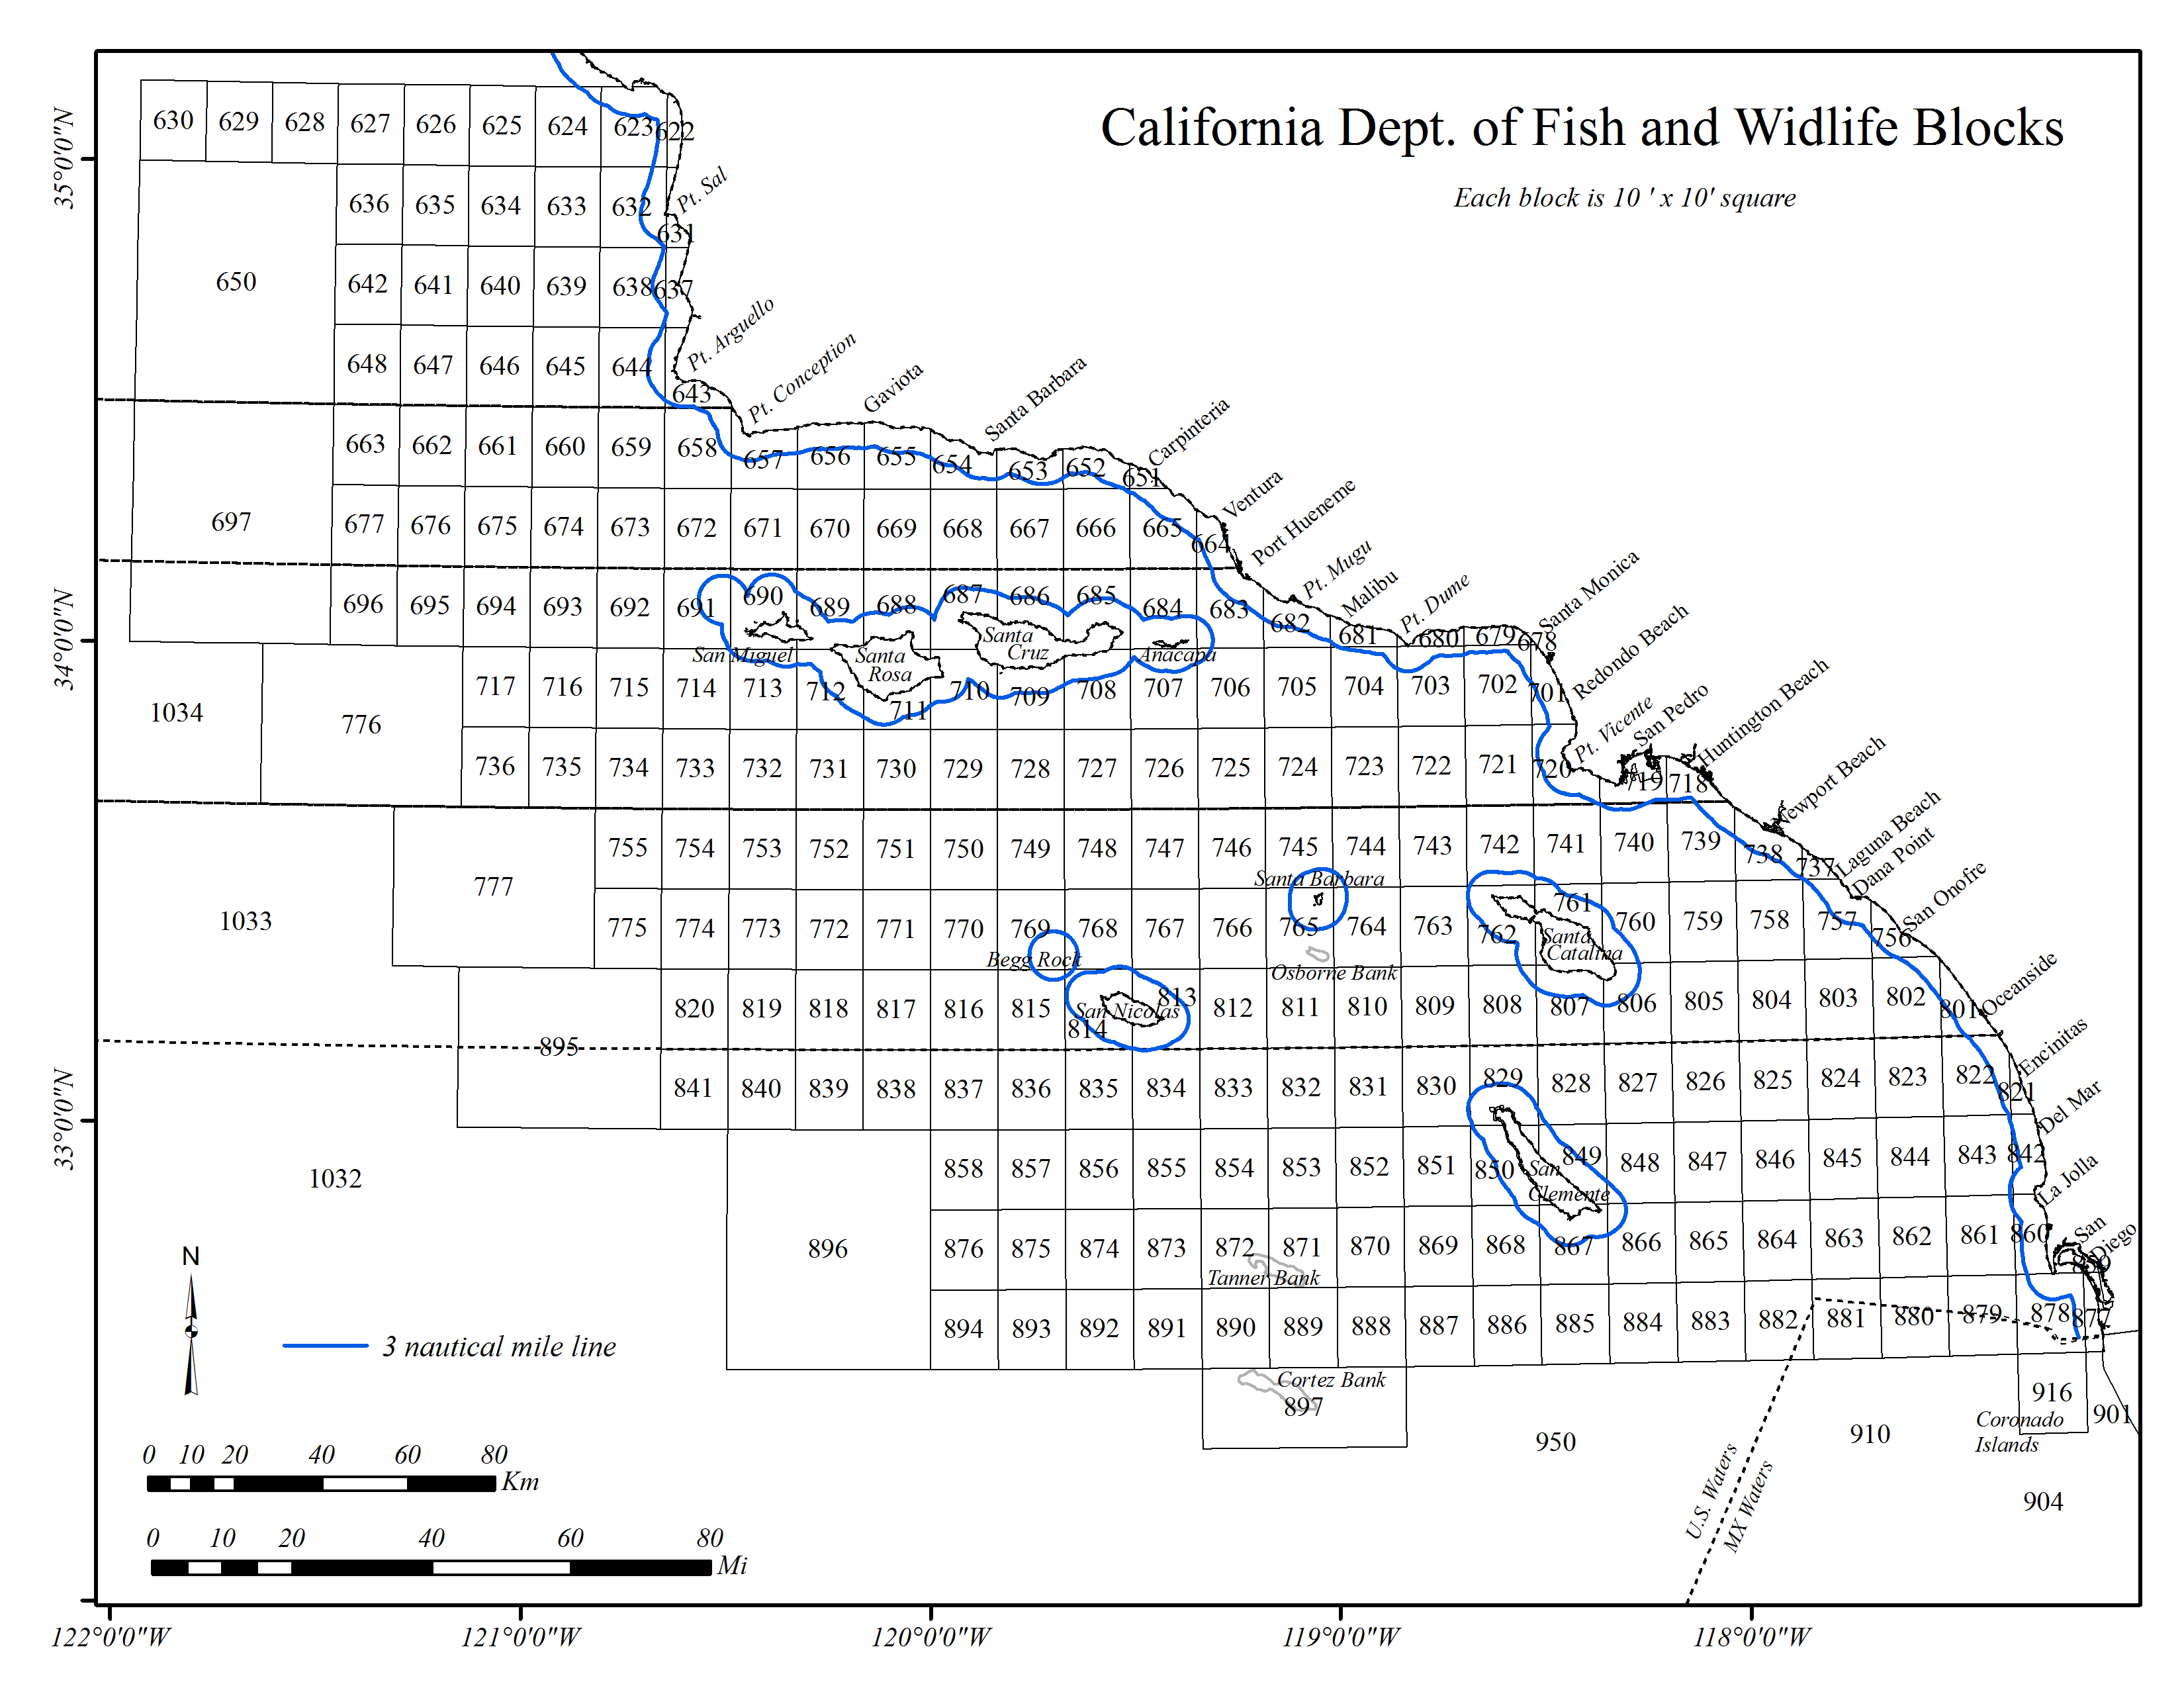
\includegraphics{Figures/boundary_map.png}
\caption{Map showing the state boundary lines for management of the
recreational fishing fleets \label{fig:boundary_map}}
\end{figure}

\begin{figure}[htbp]
\centering
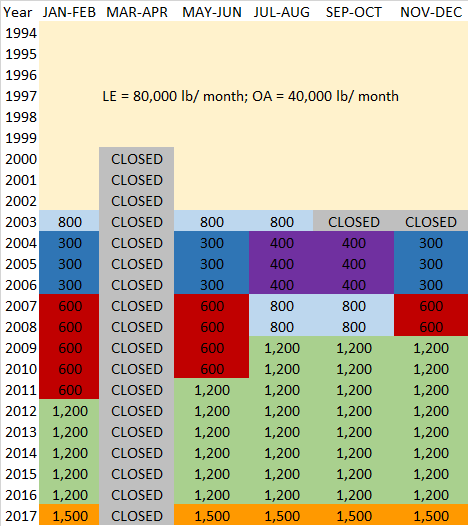
\includegraphics{Figures/Com_regs.png}
\caption{Commercial fishery regulations pertaining to limited entry (LE)
and open access (OA) fisheries in southern California. Blocks with a
numeric value indicate the bi-monthly trip limit for both LE and OA
fisheries. \label{fig:Com_regs}}
\end{figure}

\begin{figure}[htbp]
\centering
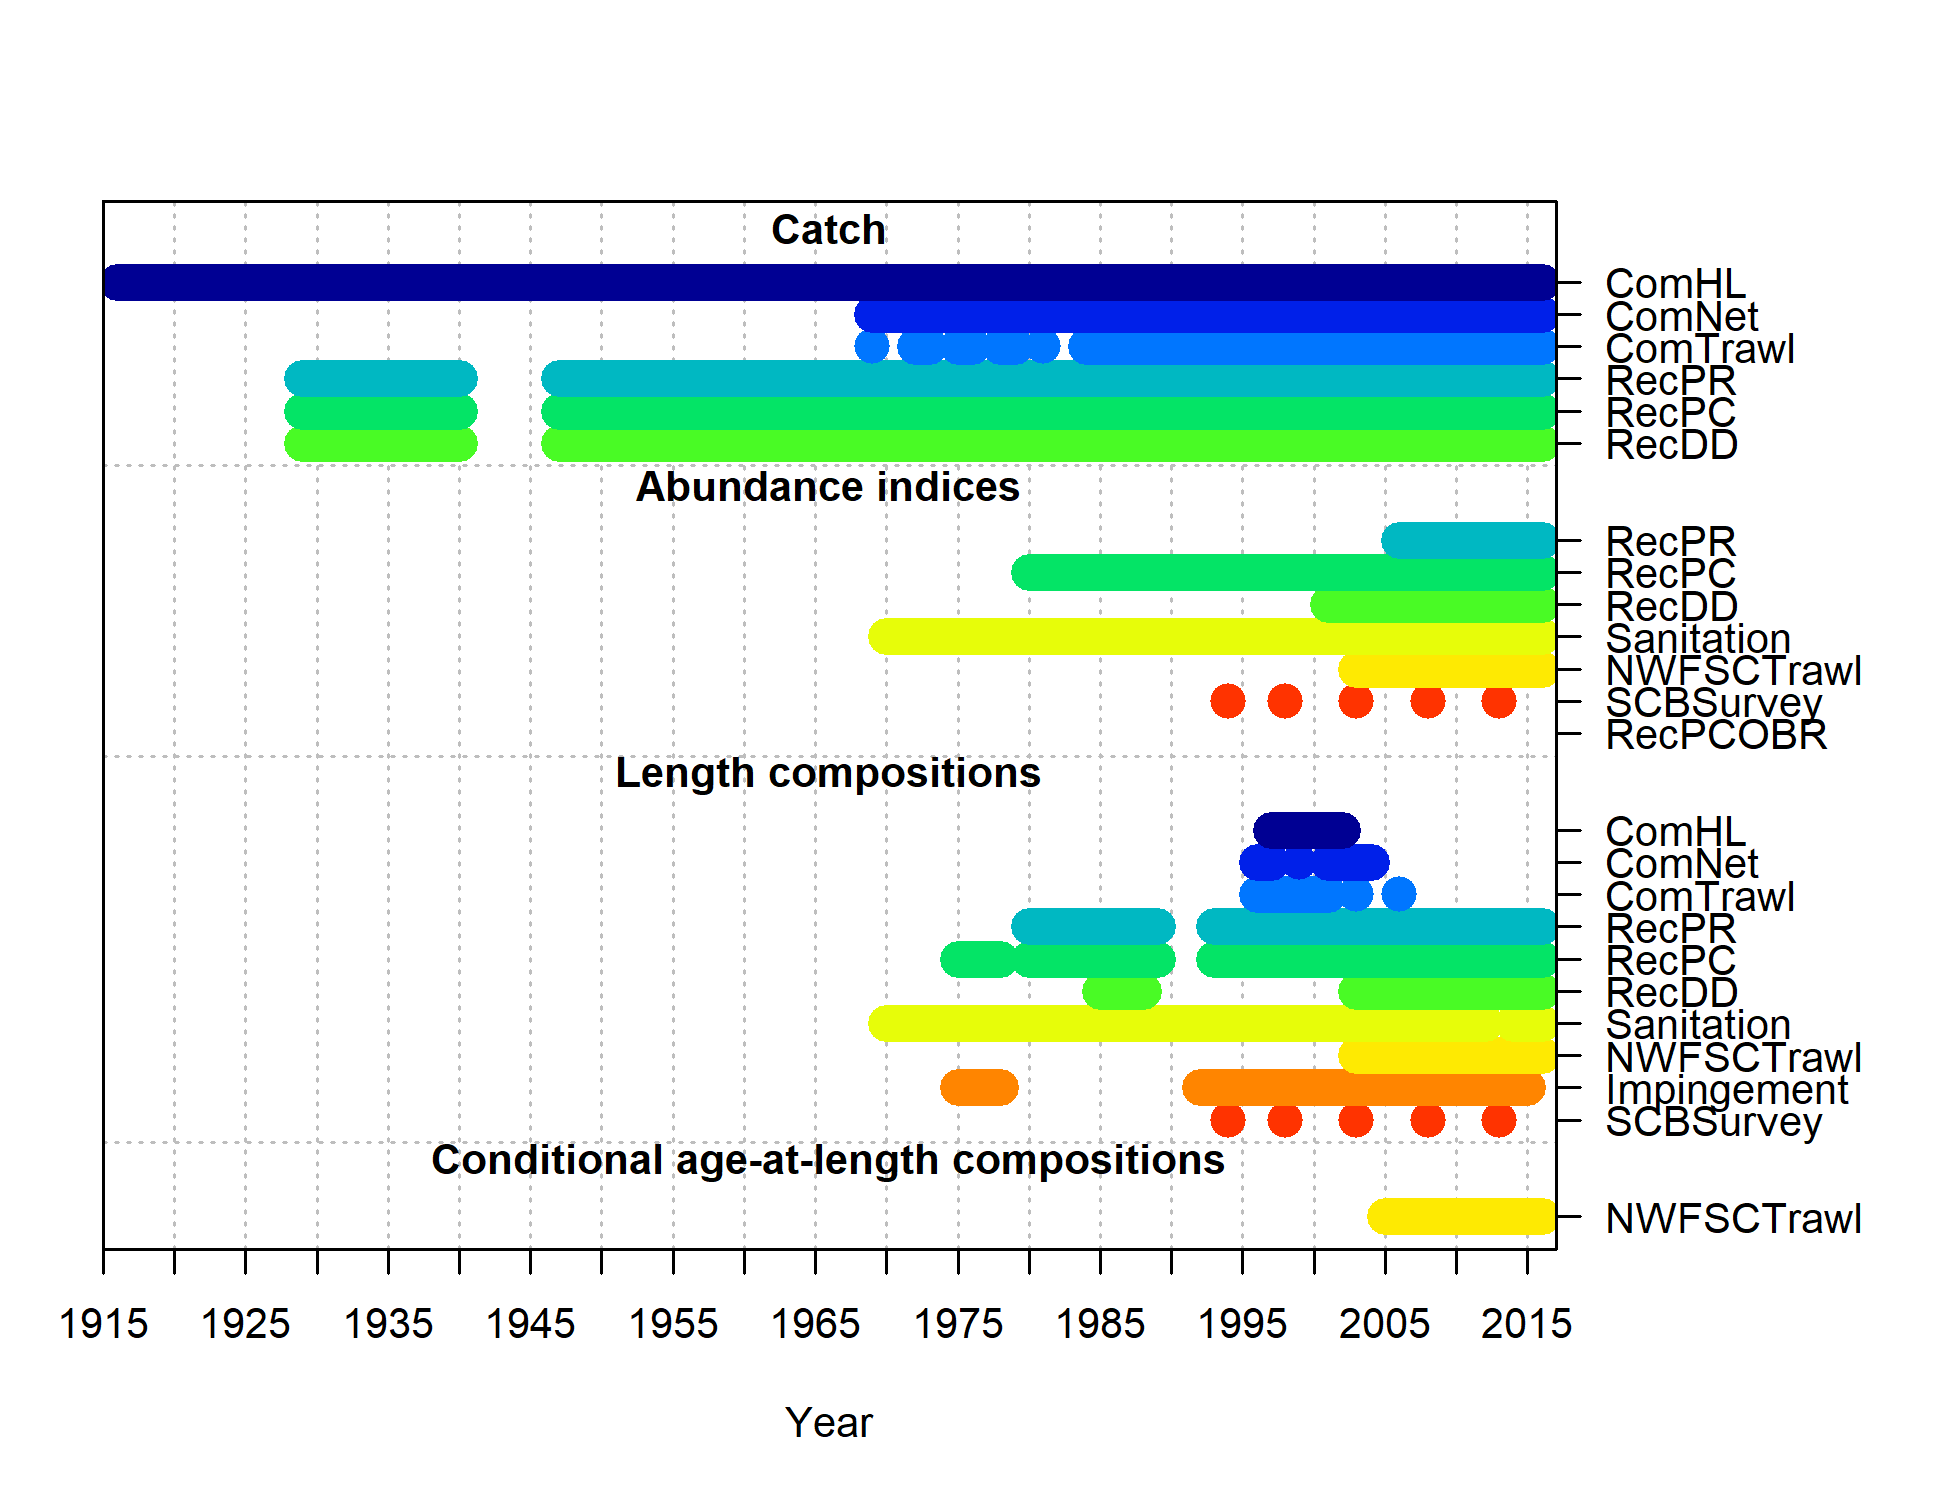
\includegraphics{r4ss/plots_mod1/data_plot.png}
\caption{Summary of data sources used in the base model.
\label{fig:data_plot}}
\end{figure}

\FloatBarrier

\begin{figure}[htbp]
\centering
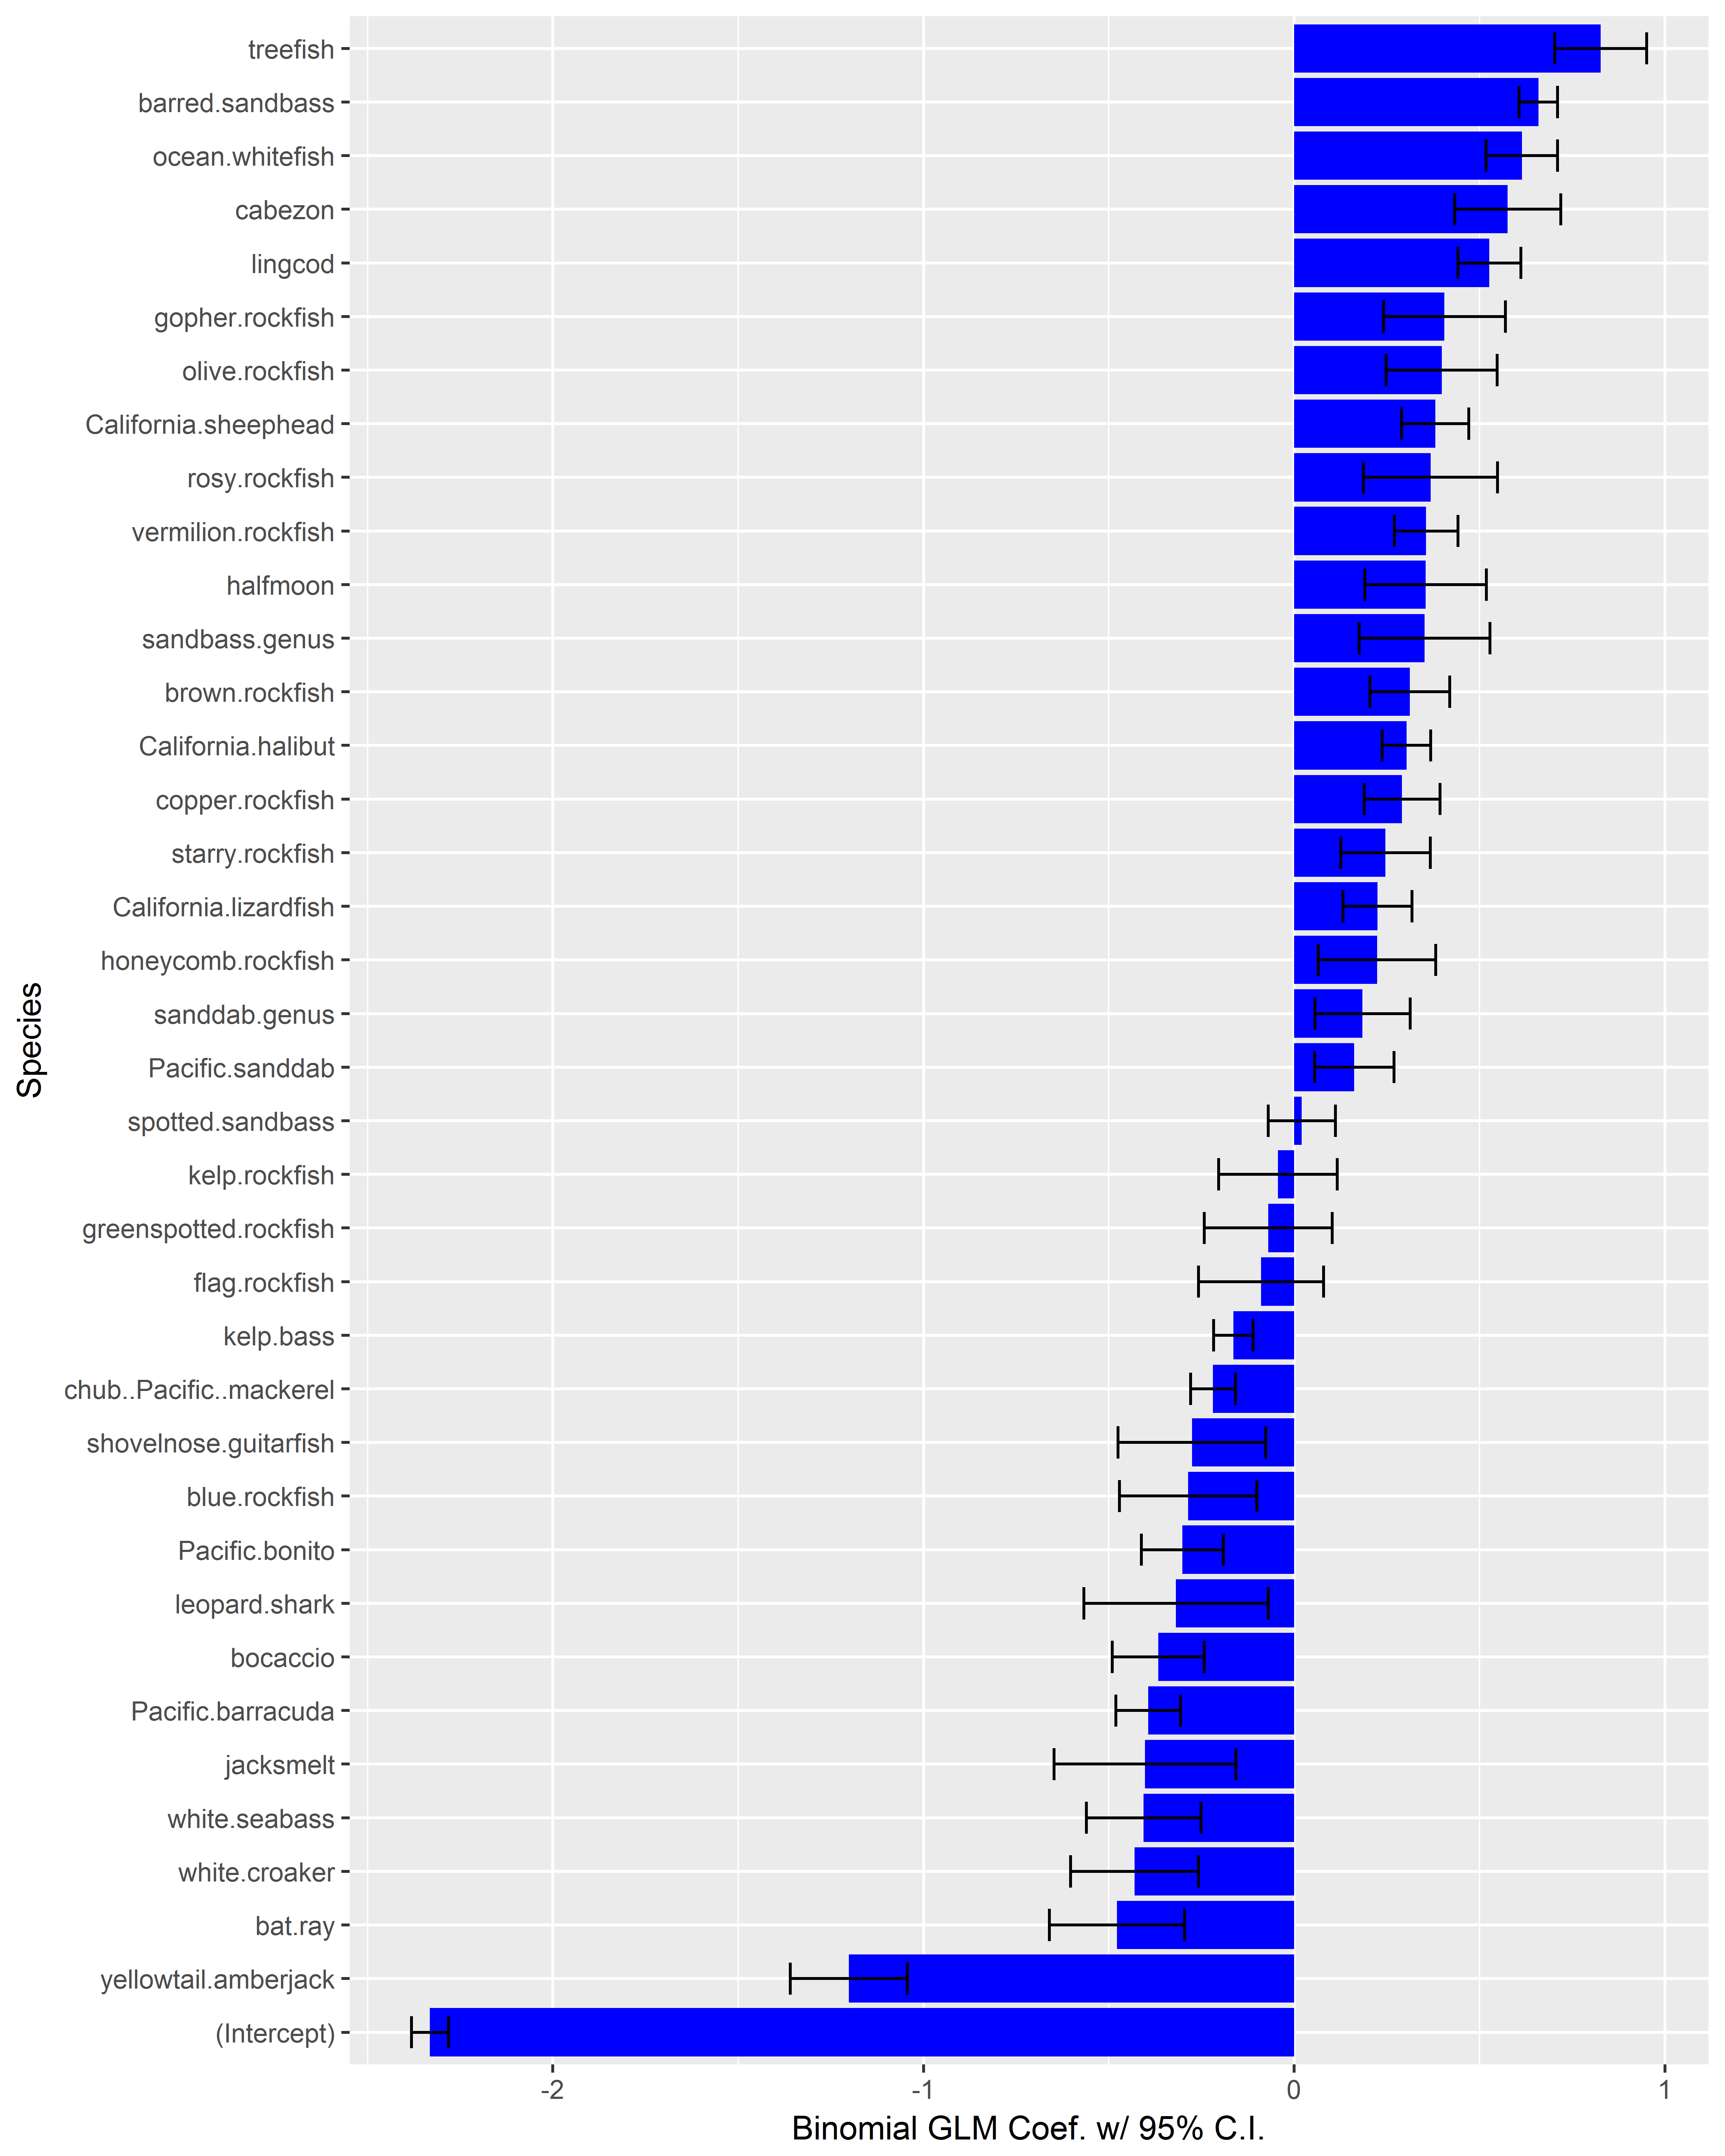
\includegraphics{Figures/Fleet4_RecPR_SMcoef.png}
\caption{Species coefficients from the binomial GLM for presence/absence
of California scorpionfish in the Marine Recreational Fisheries
Statistics Survey (MRFSS) private mode dockside survey data set.
Horizontal bars are 95\% confidence intervals.
\label{fig:Fleet4_RecPR_dockside_SM}}
\end{figure}

\begin{figure}[htbp]
\centering
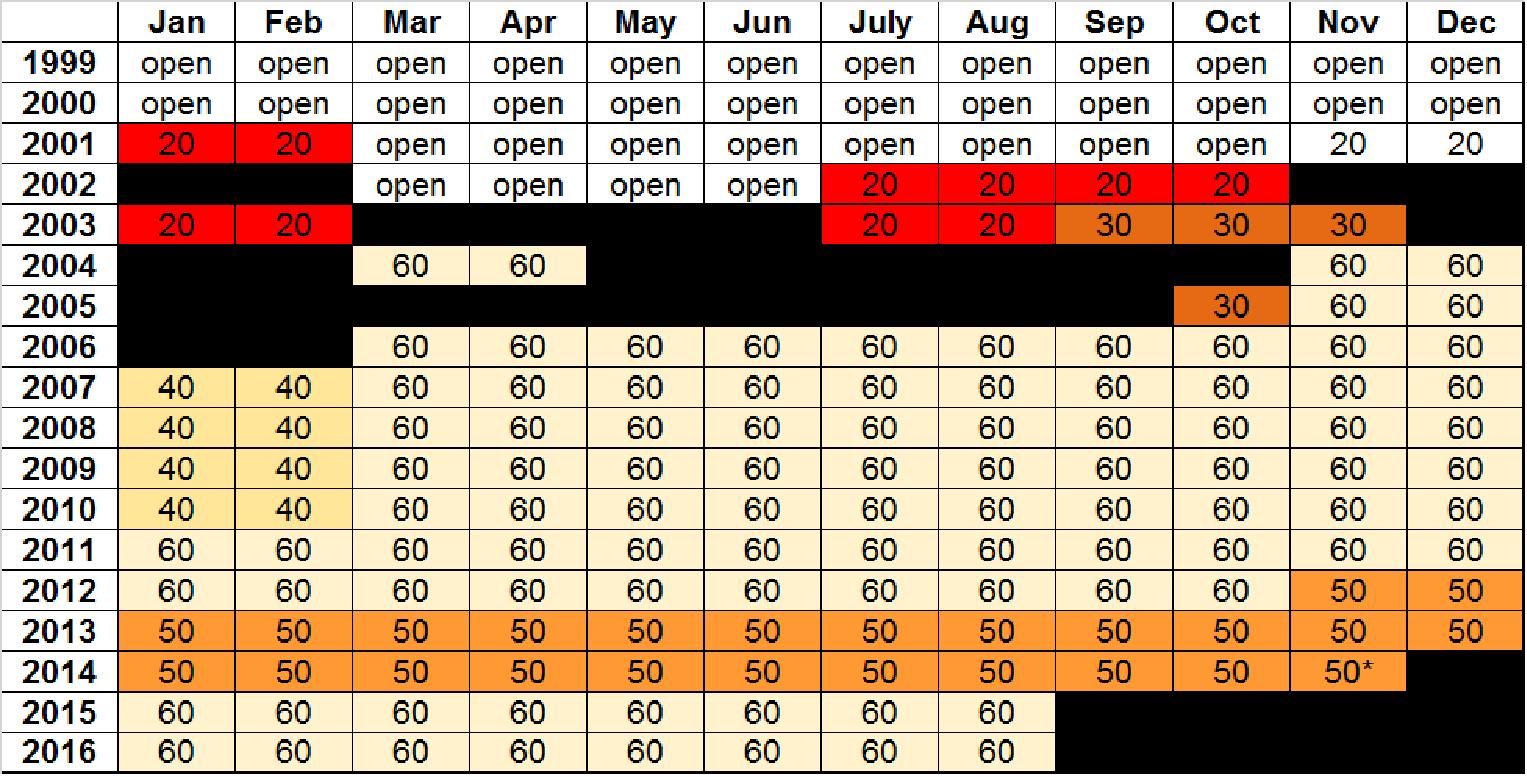
\includegraphics{Figures/Rec_regs.pdf}
\caption{A summary of the monthly recreational regulations for
California scorpionfish in southern California. Cells with ``open''
indicate no depth restriction, black cells indicate the fishery is
closed, and cells with a number indicate the depth restriction in
fathoms, e.g., 20 = retained catch allowed in less than 20 fathoms.
*Fishery closed on November 15, 2014. \label{fig:recregs}}
\end{figure}

\begin{figure}[htbp]
\centering
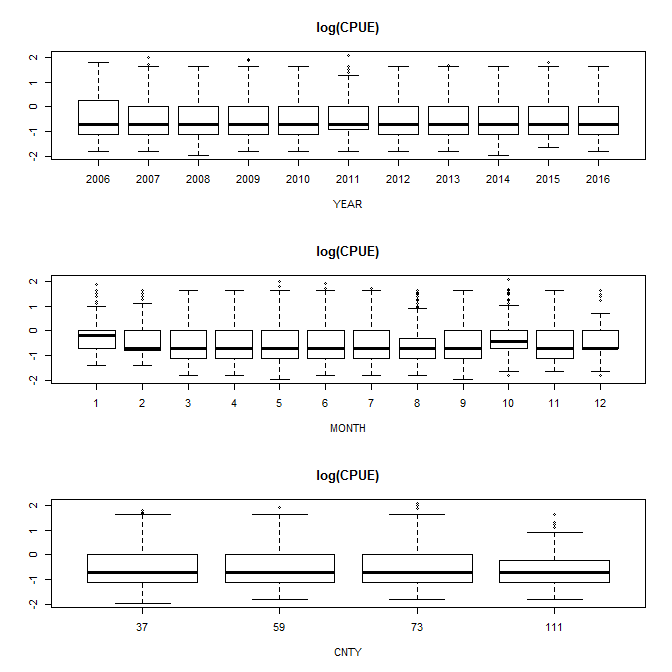
\includegraphics{Figures/Fleet4_RecPR_dockside_lograwCPUE.png}
\caption{Boxplots of the raw log CPUE by year for each of the three
factors considered in the deltaGLM model, county, month and year.
\label{fig:Fleet4_RecPR_dockside_lograwCPUE}}
\end{figure}

\FloatBarrier 

\begin{figure}[htbp]
\centering
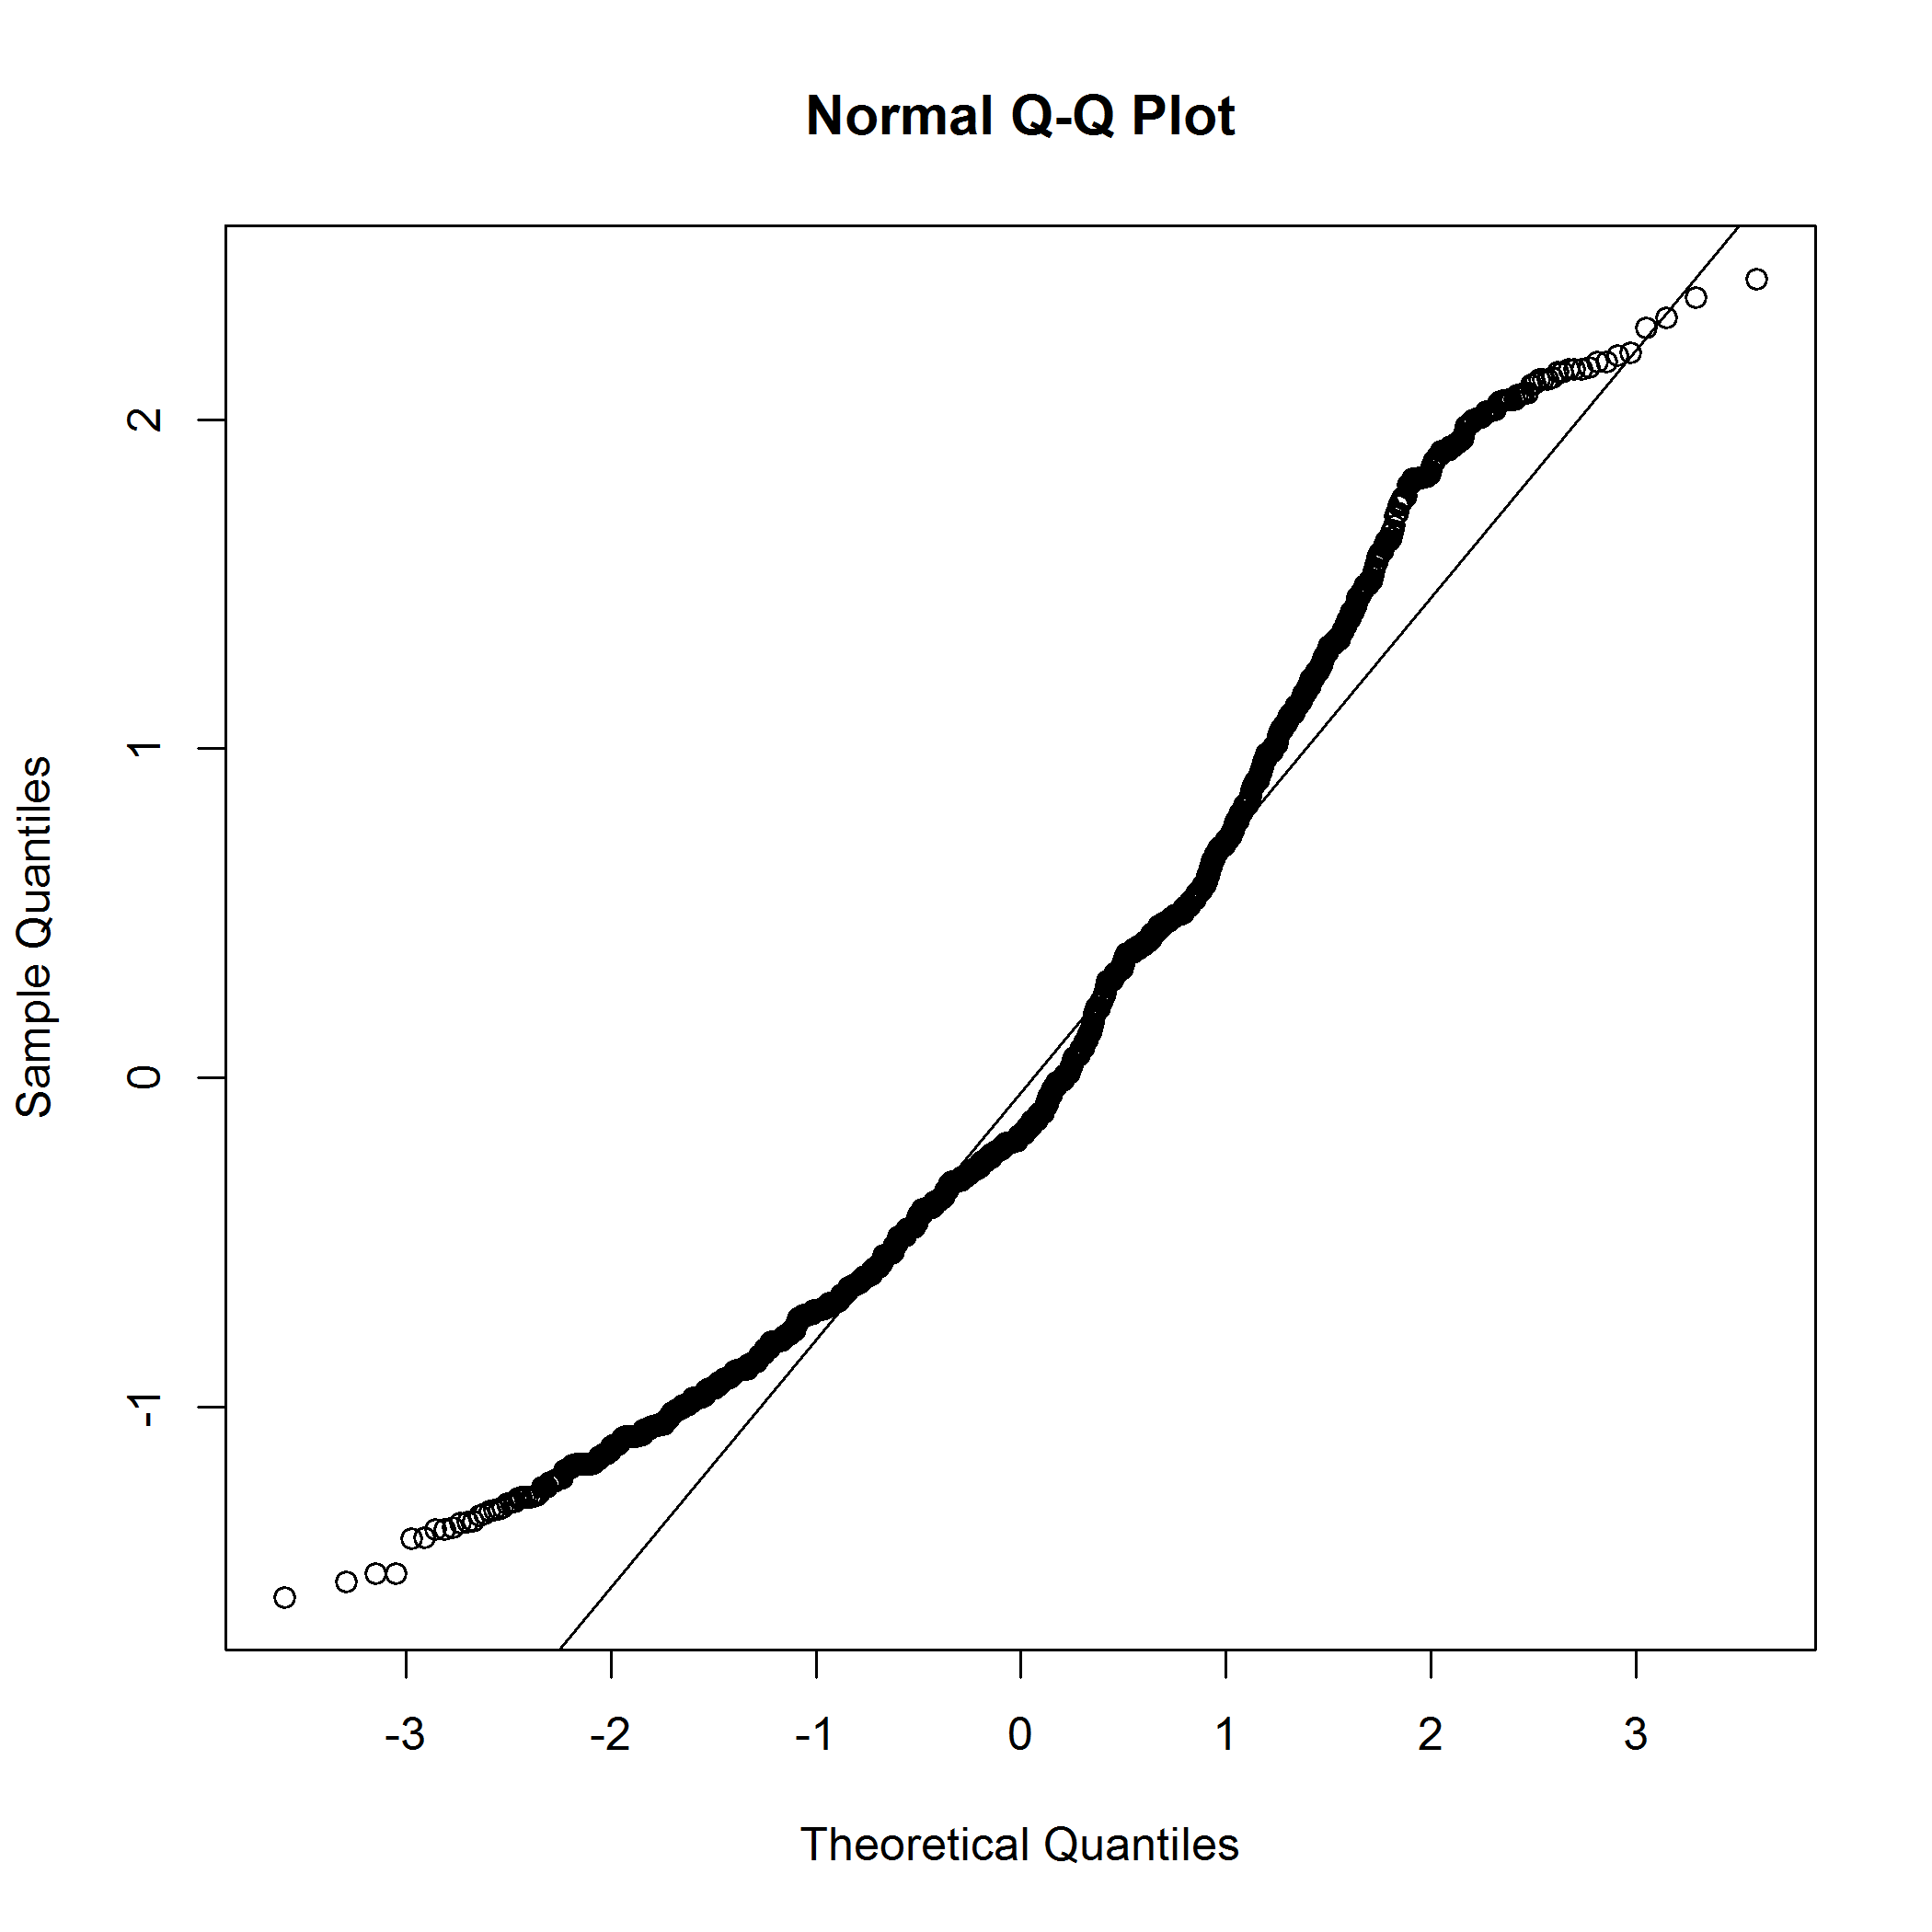
\includegraphics{Figures/Fleet4_RecPR_dockside_QQ.png}
\caption{Q-Q plot used to evaluate the fit of the lognormal (positive
encounters) of California scorpionfish from the California Recreational
Fisheries Statistics Survey (CRFS) private mode dockside survey data
set. \label{fig:Fleet4_RecPR_dockside_QQ}}
\end{figure}

\begin{figure}[htbp]
\centering
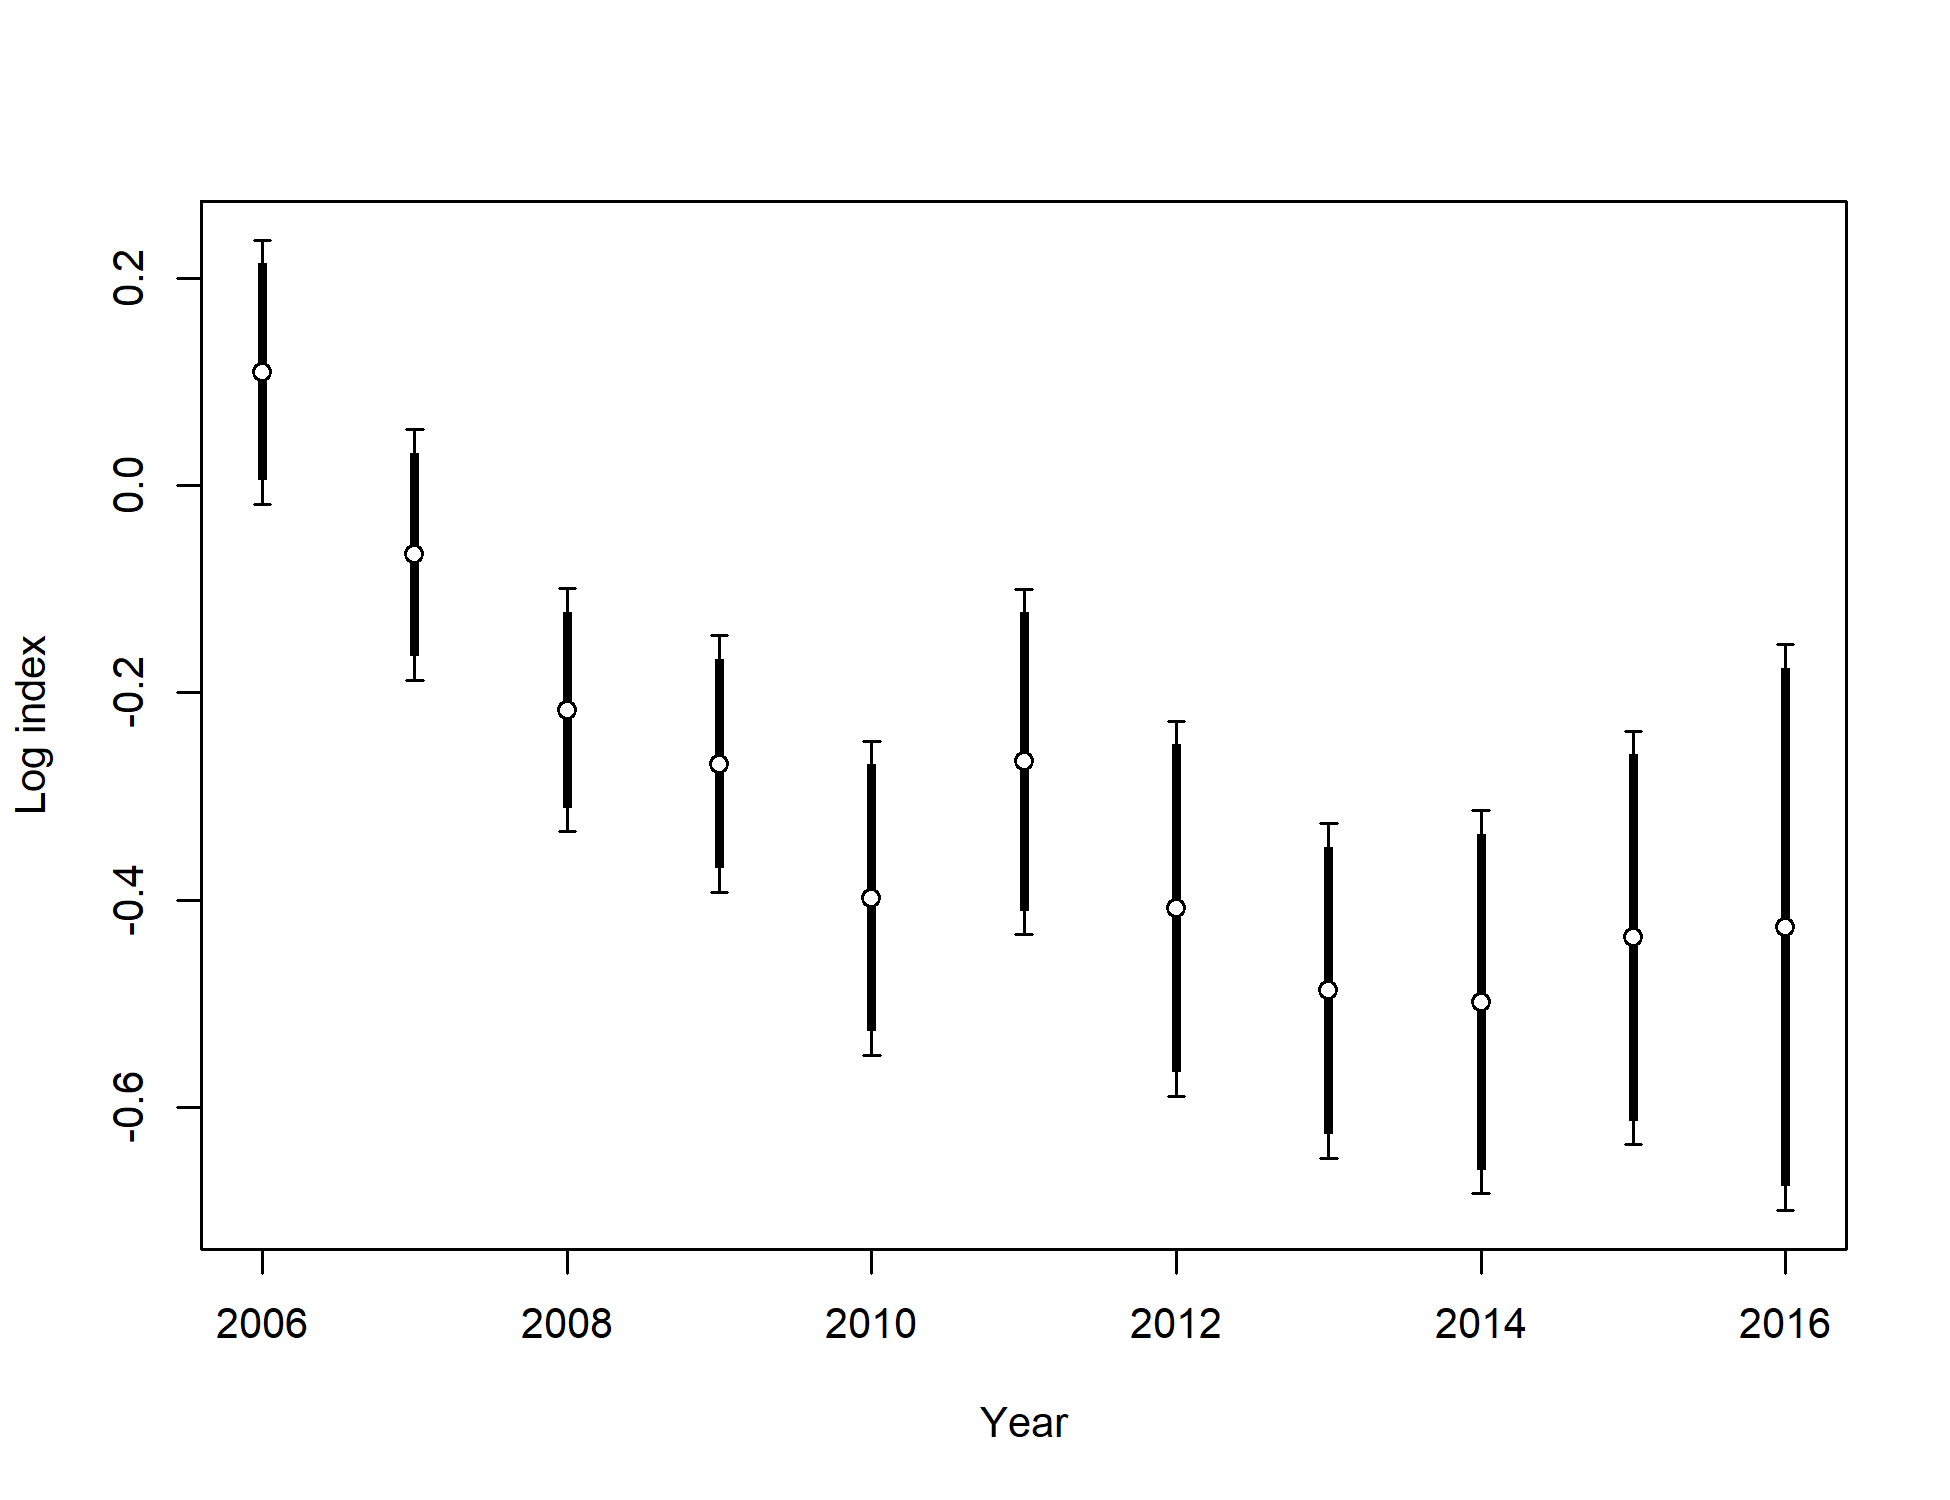
\includegraphics{r4ss/plots_mod1/index4_logcpuedata_RecPR.png}
\caption{Standardized index on log scale for the recreational private
mode dockside survey data set. Lines indicate 95\% uncertainty interval
around index values. Thicker lines indicate input uncertainty before
addition of estimated additional uncertainty parameter.
\label{fig:index4_logcpuedata_RecPR}}
\end{figure}

\FloatBarrier

\FloatBarrier

\begin{figure}[htbp]
\centering
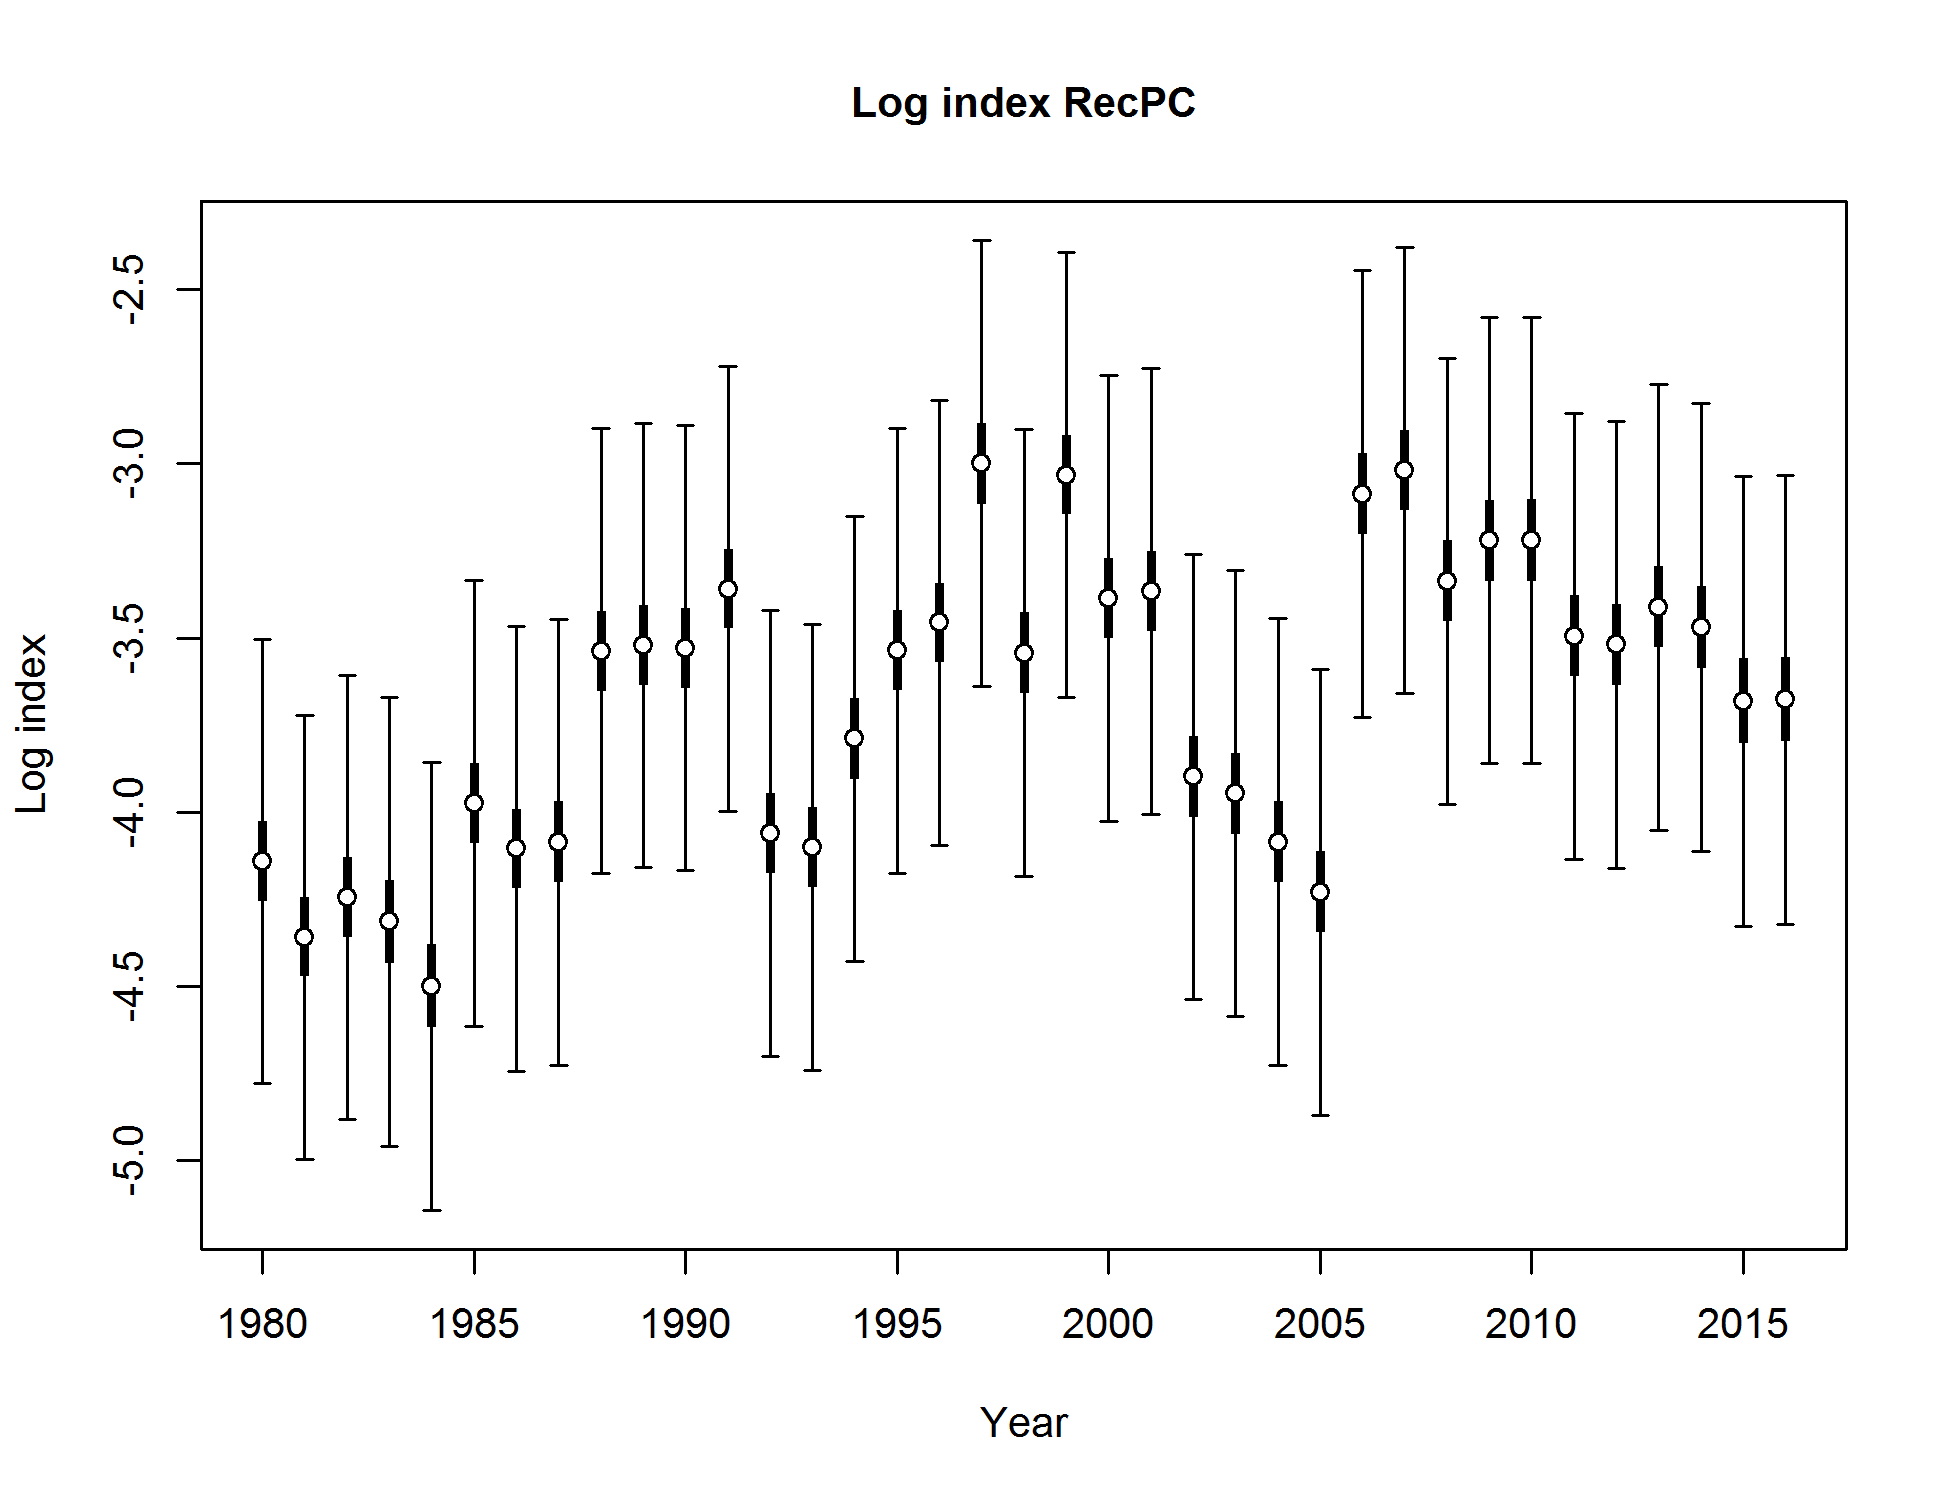
\includegraphics{r4ss/plots_mod1/index4_logcpuedata_RecPC.png}
\caption{Standardized index on the log scale for the recreational CPFV
logbook retained catches. Lines indicate 95\% uncertainty interval
around index values. Thicker lines indicate input uncertainty before
addition of estimated additional uncertainty parameter.
\label{fig:index4_logcpuedata_RecPC}}
\end{figure}

\FloatBarrier

\begin{figure}[htbp]
\centering
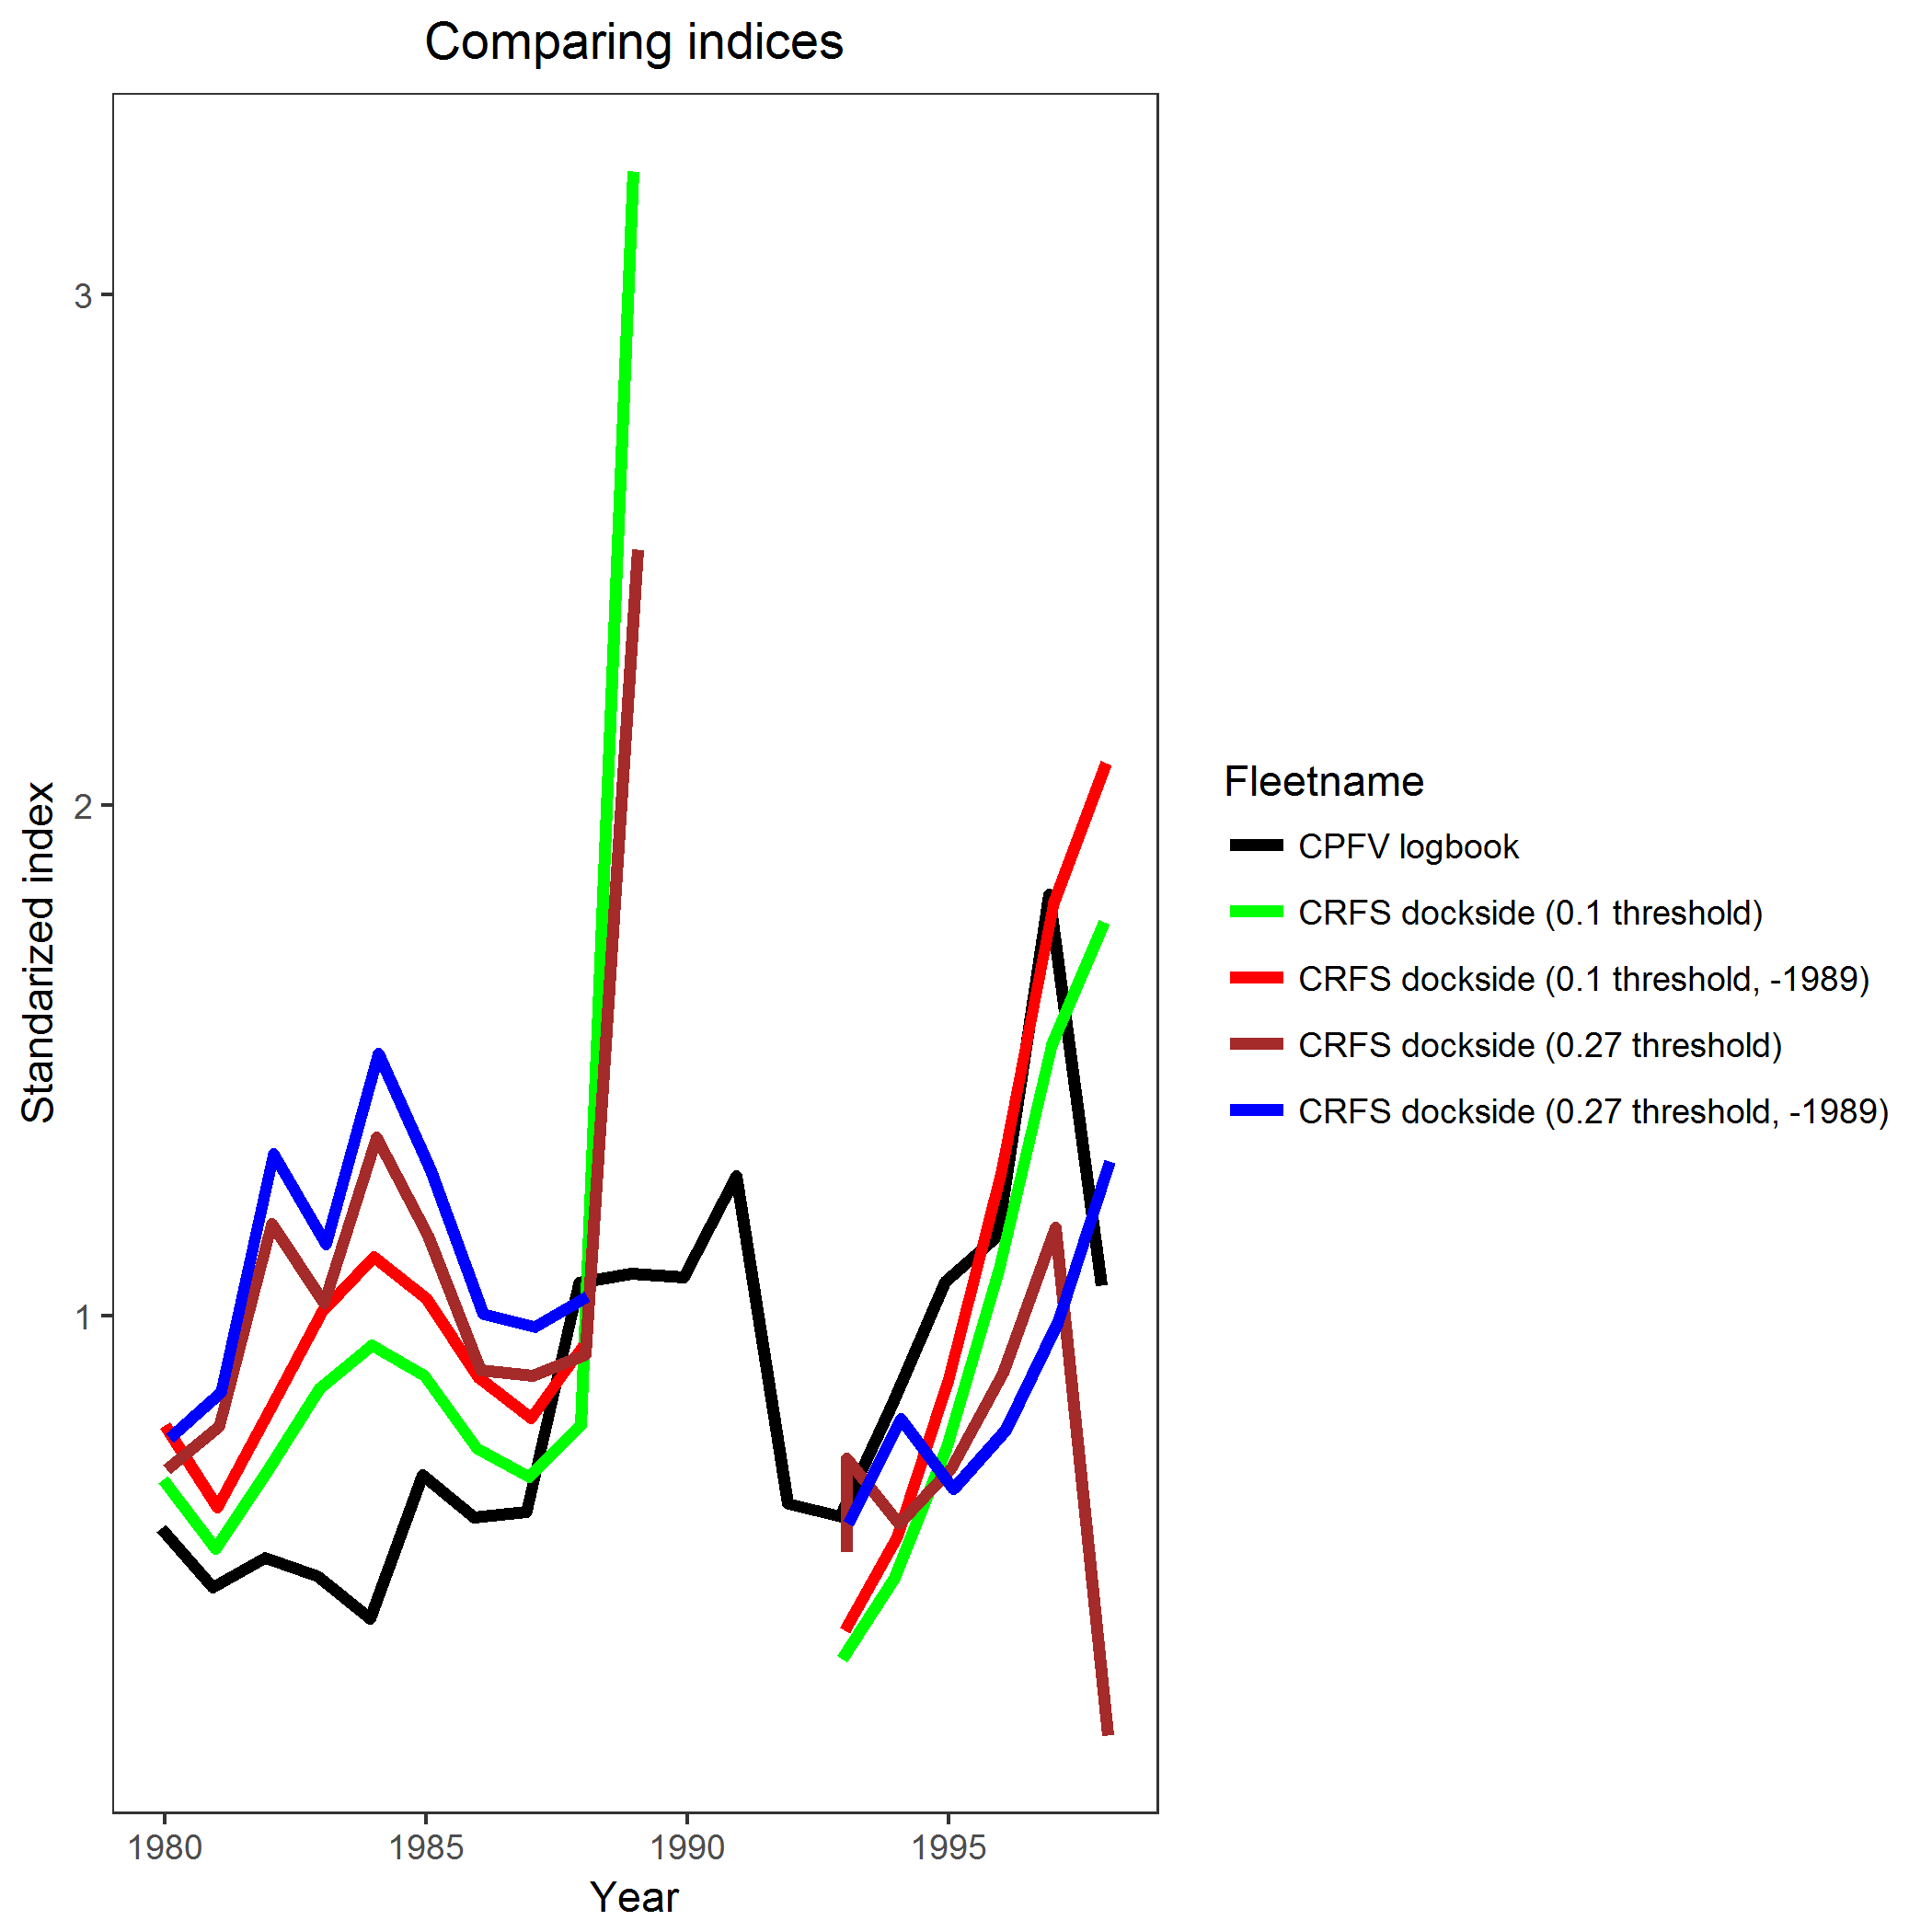
\includegraphics{Figures/Fleet5_RecPC_dockside_index_compare.png}
\caption{Comparison of standardized indices using two different
threshold levels (0.27 and 0.1) from the Stephens-MacCall filtering, and
including or excluding the year 1989.
\label{fig:Fleet5_RecPC_dockside_index_compare}}
\end{figure}

\FloatBarrier

\begin{figure}[htbp]
\centering
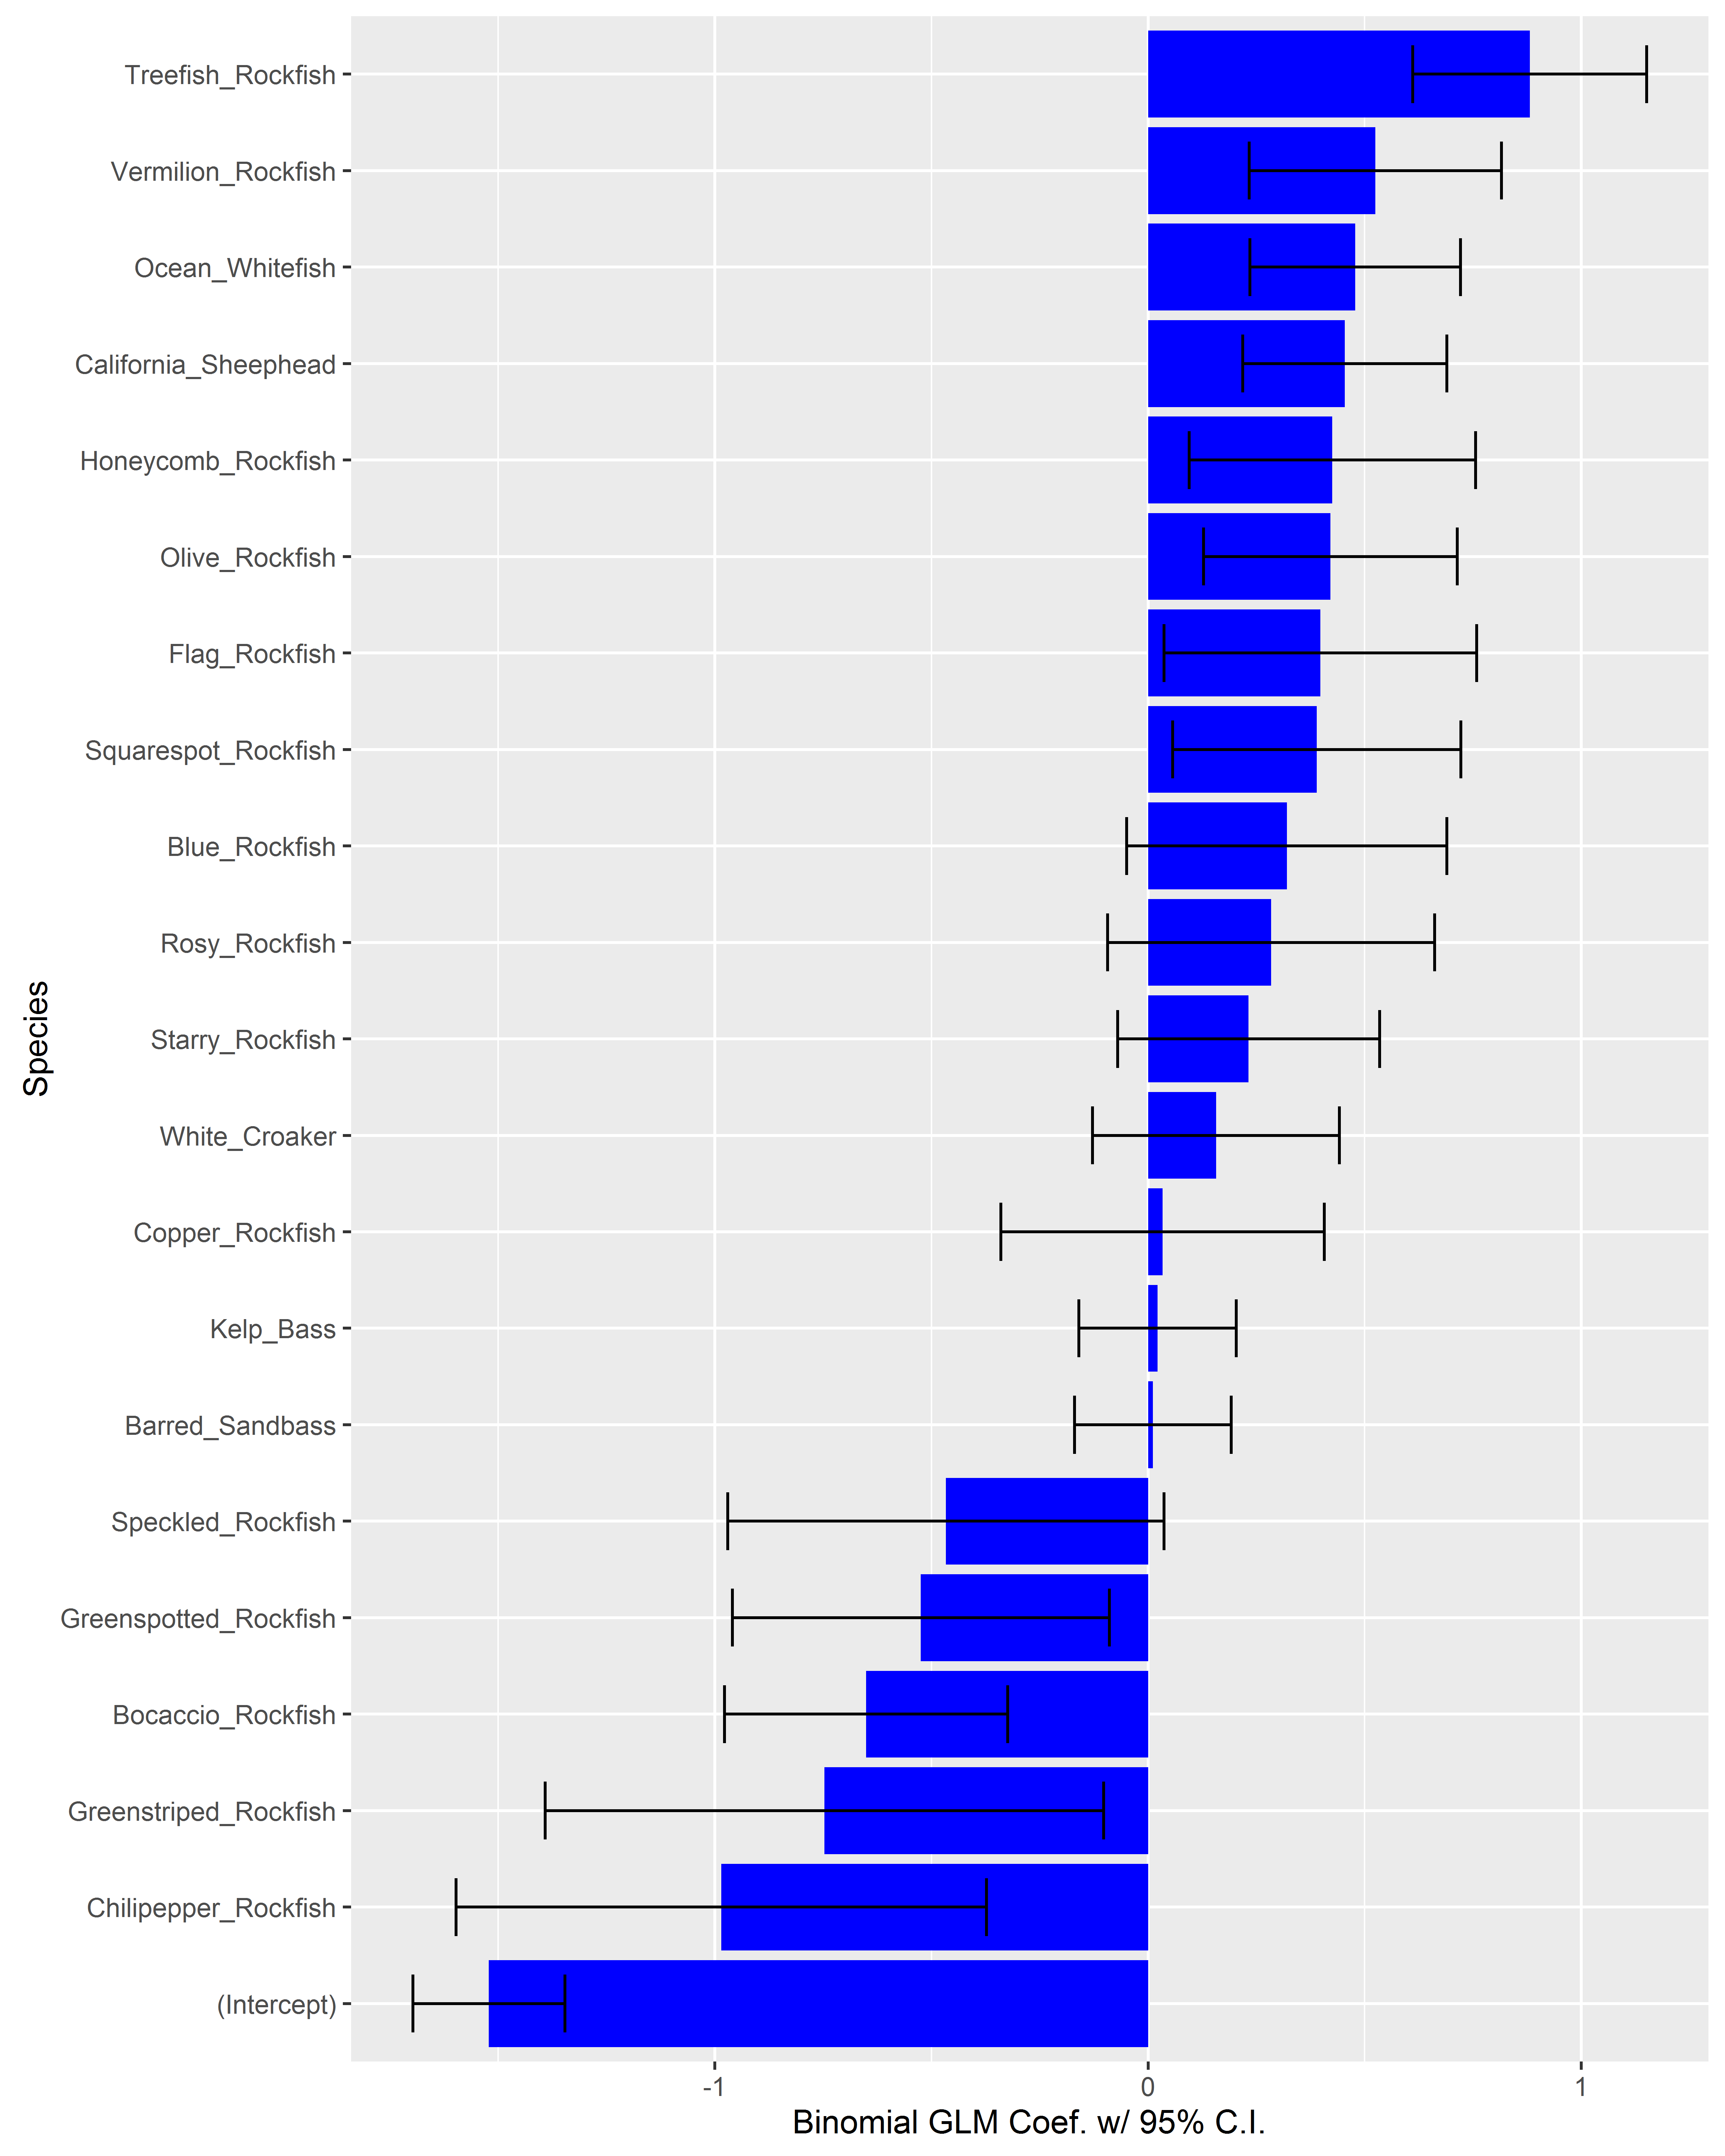
\includegraphics{Figures/Fleet5_RecPC_dockside_SM.png}
\caption{Species coefficients from the binomial GLM for presence/absence
of California scorpionfish in the Marine Recreational Fisheries
Statistics Survey (MRFSS) party/charter mode dockside survey data set.
Horizontal bars are 95\% confidence intervals.
\label{fig:Fleet5_RecPC_docksideSM}}
\end{figure}

\begin{figure}[htbp]
\centering
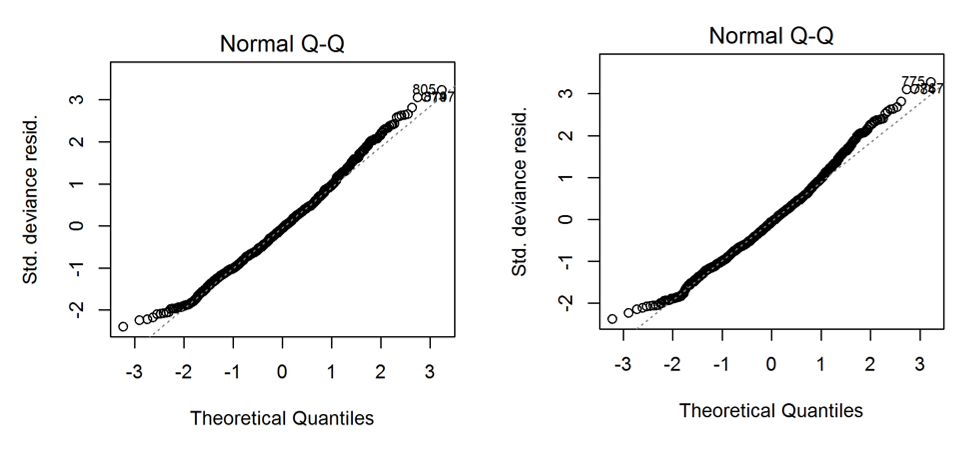
\includegraphics{Figures/Fleet5_RecPC_dockside_QQ.png}
\caption{Q-Q plot used to validate the goodness of fit of the lognormal
portion (positive catch) of the Marine Recreational Fisheries Statistics
Survey (MRFSS) party/charter dockside survey, for thresholds of 0.27
(left) and 0.10 (right) from the Stephens-MacCall filter.
\label{fig:Fleet5_RecPC_docksideQQ}}
\end{figure}

\FloatBarrier

\begin{figure}[htbp]
\centering
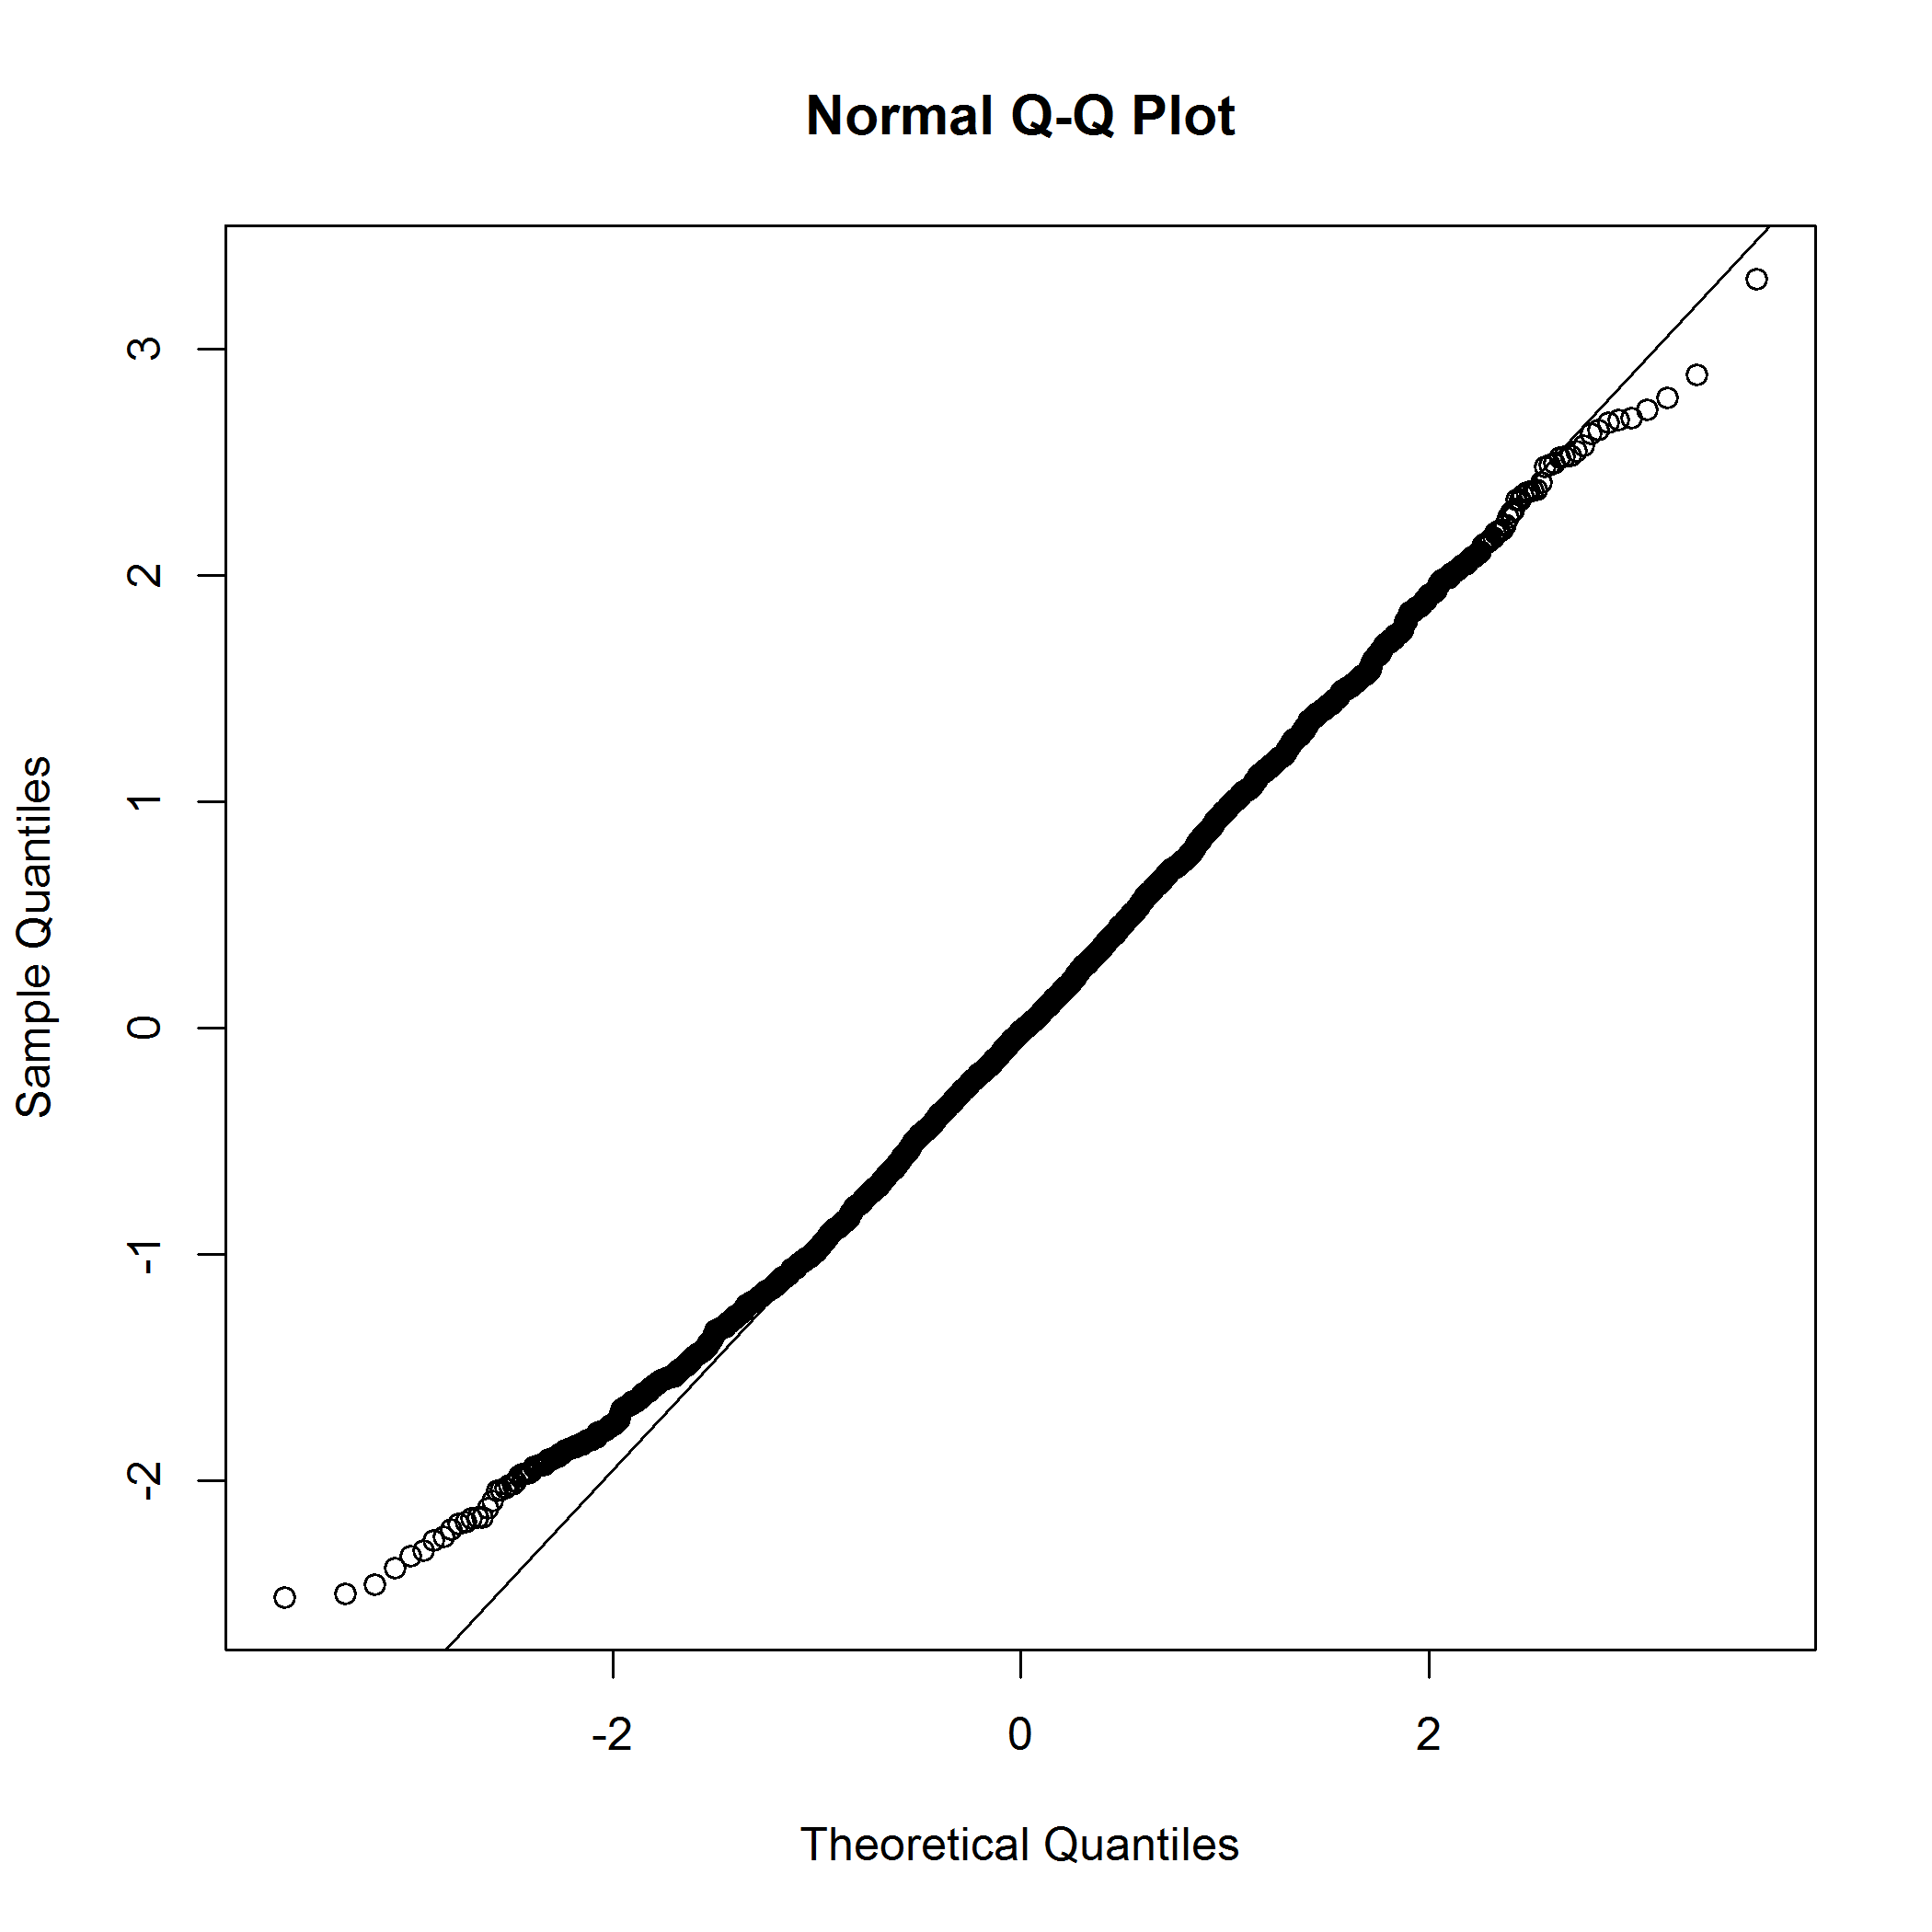
\includegraphics{Figures/Fleet6_RecDD_QQ.png}
\caption{Q-Q plot used to validate the goodness of fit of the lognormal
model for the CPFV onboard observer discarded only catch.
\label{fig:Fleet6_RecDD_QQ}}
\end{figure}

\begin{figure}[htbp]
\centering
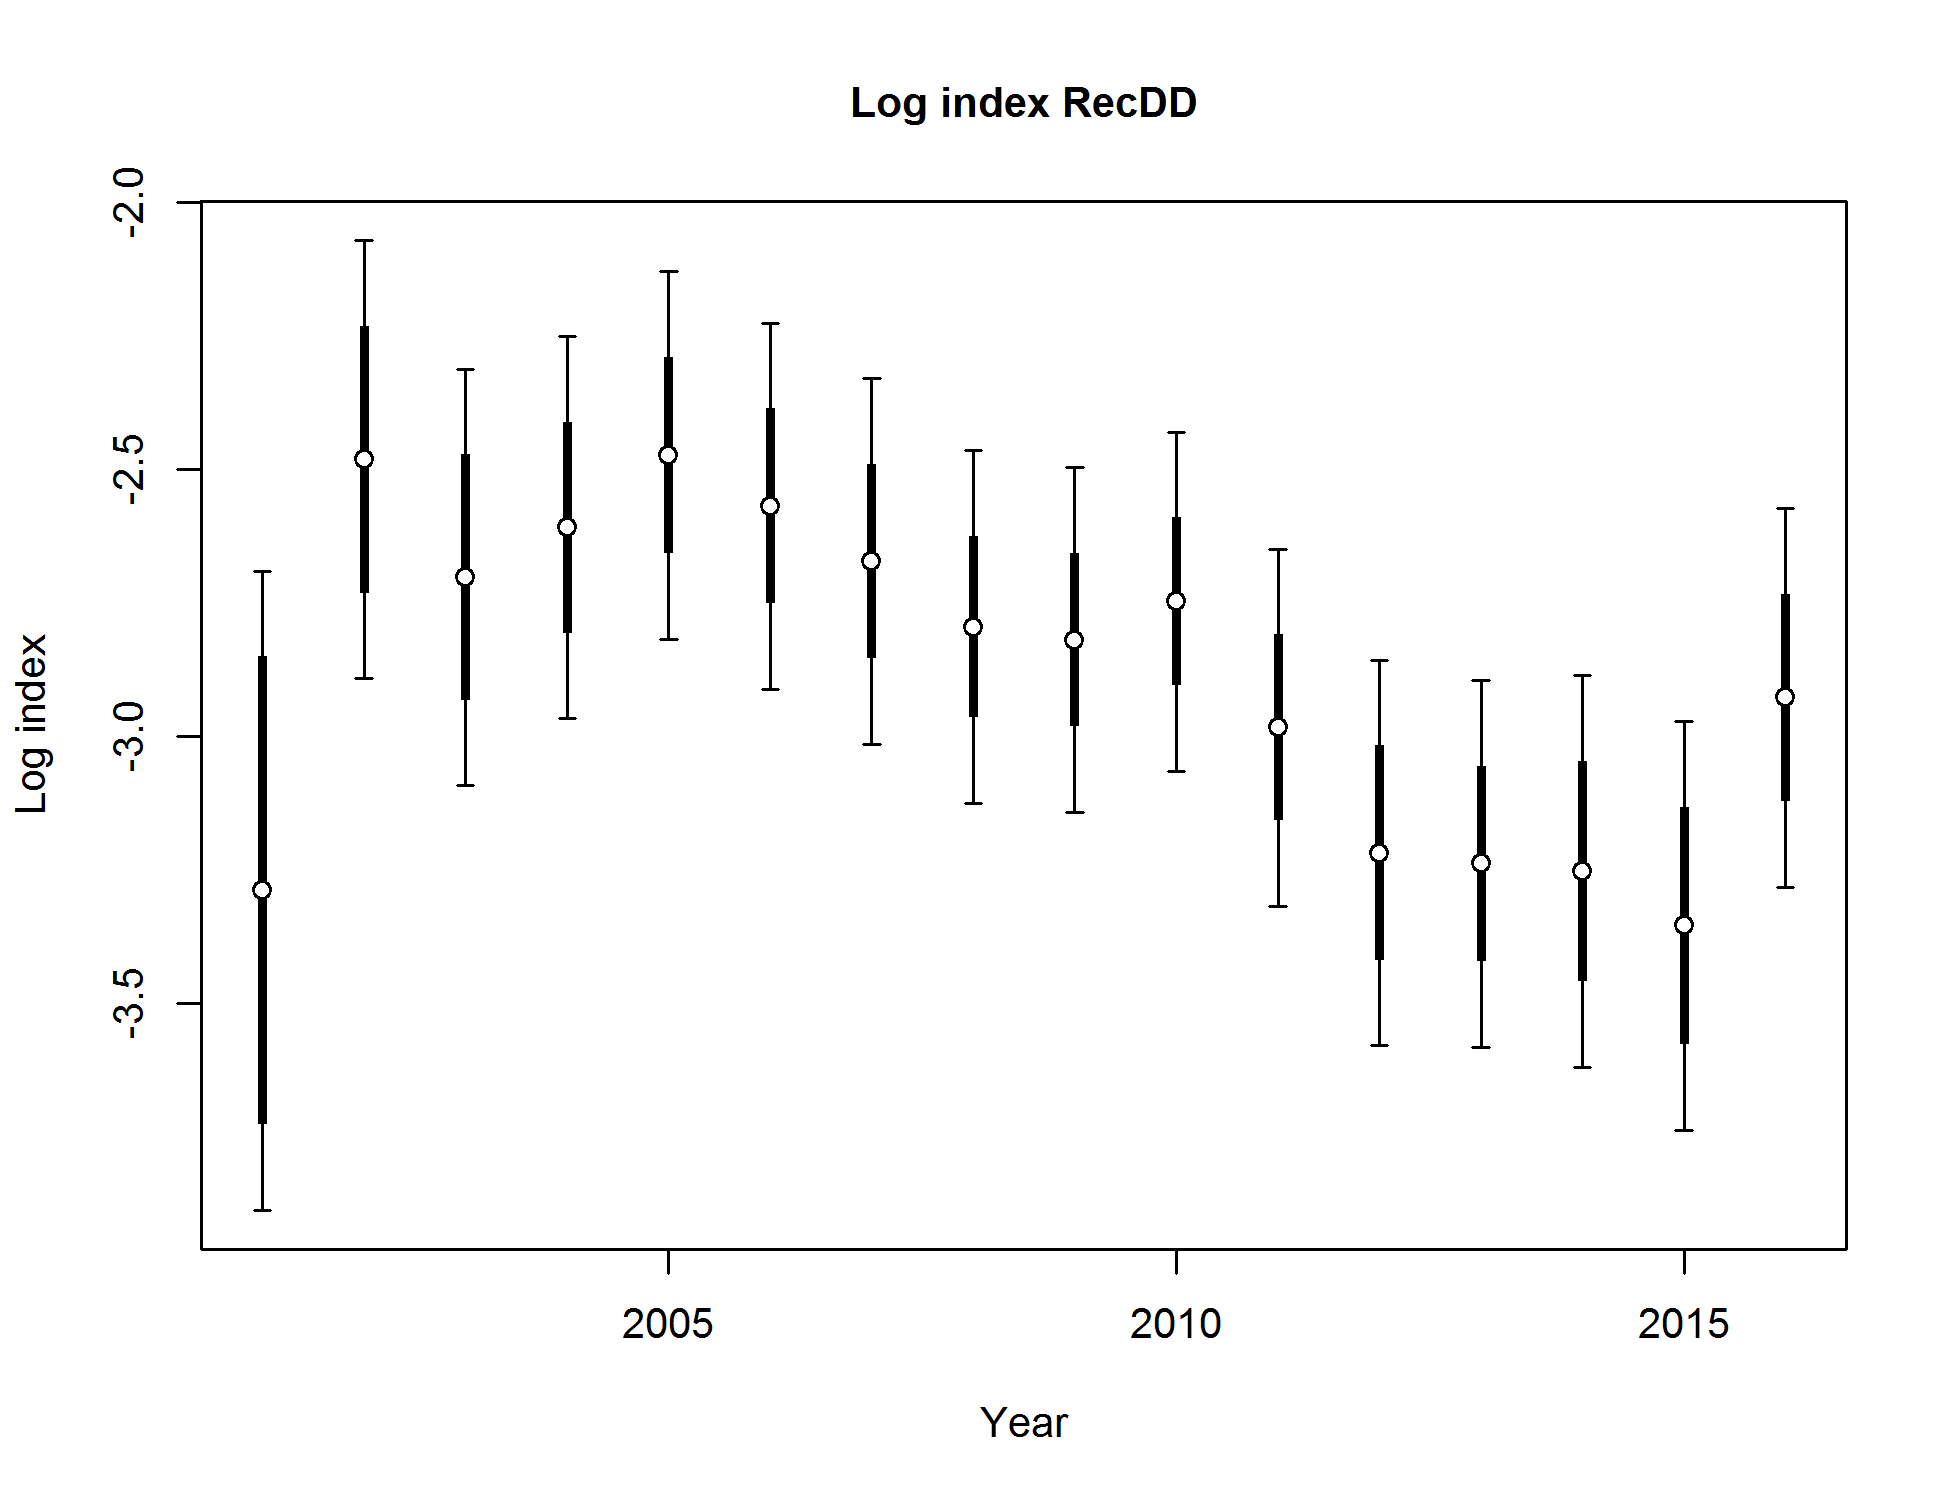
\includegraphics{r4ss/plots_mod1/index4_logcpuedata_RecDD.png}
\caption{Standardized index on the log scale for the recreational CPFV
onboard observer discarded catch index. Lines indicate 95\% uncertainty
interval around index values. Thicker lines indicate input uncertainty
before addition of estimated additional uncertainty parameter.
\label{fig:Fleet6_index4_logcpuedata_RecDD}}
\end{figure}

\begin{figure}[htbp]
\centering
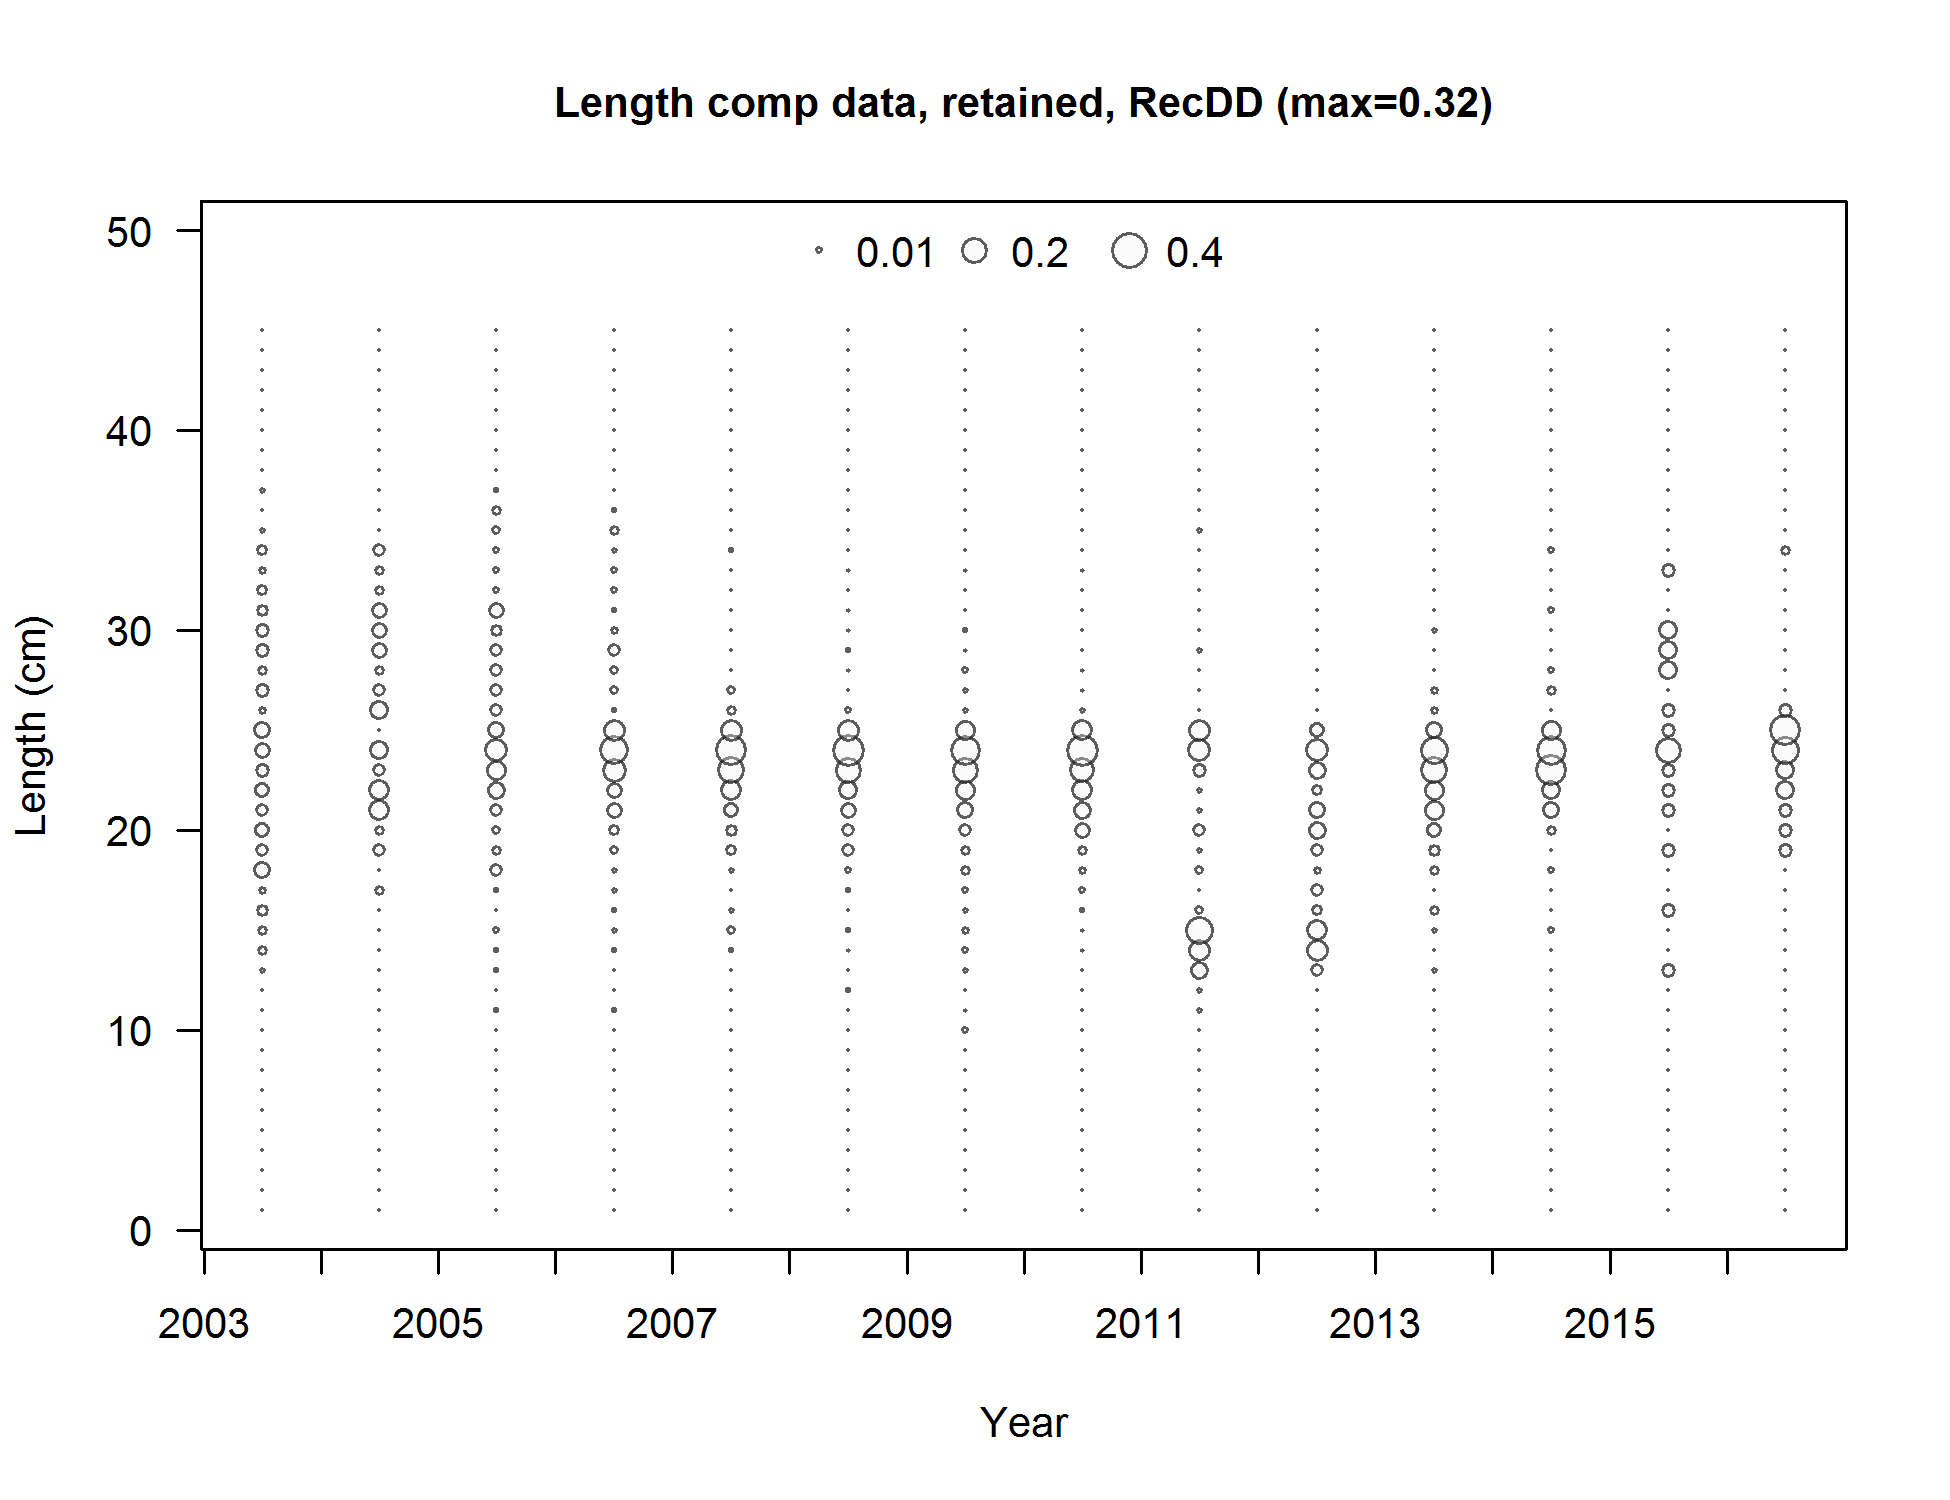
\includegraphics{r4ss/plots_mod1/comp_lendat_bubflt6mkt2.png}
\caption{Length frequency distributions from the onboard observer
discard-only catch. \label{fig:Fleet6_comp_lendat_bubflt6mkt2}}
\end{figure}

\begin{figure}[htbp]
\centering
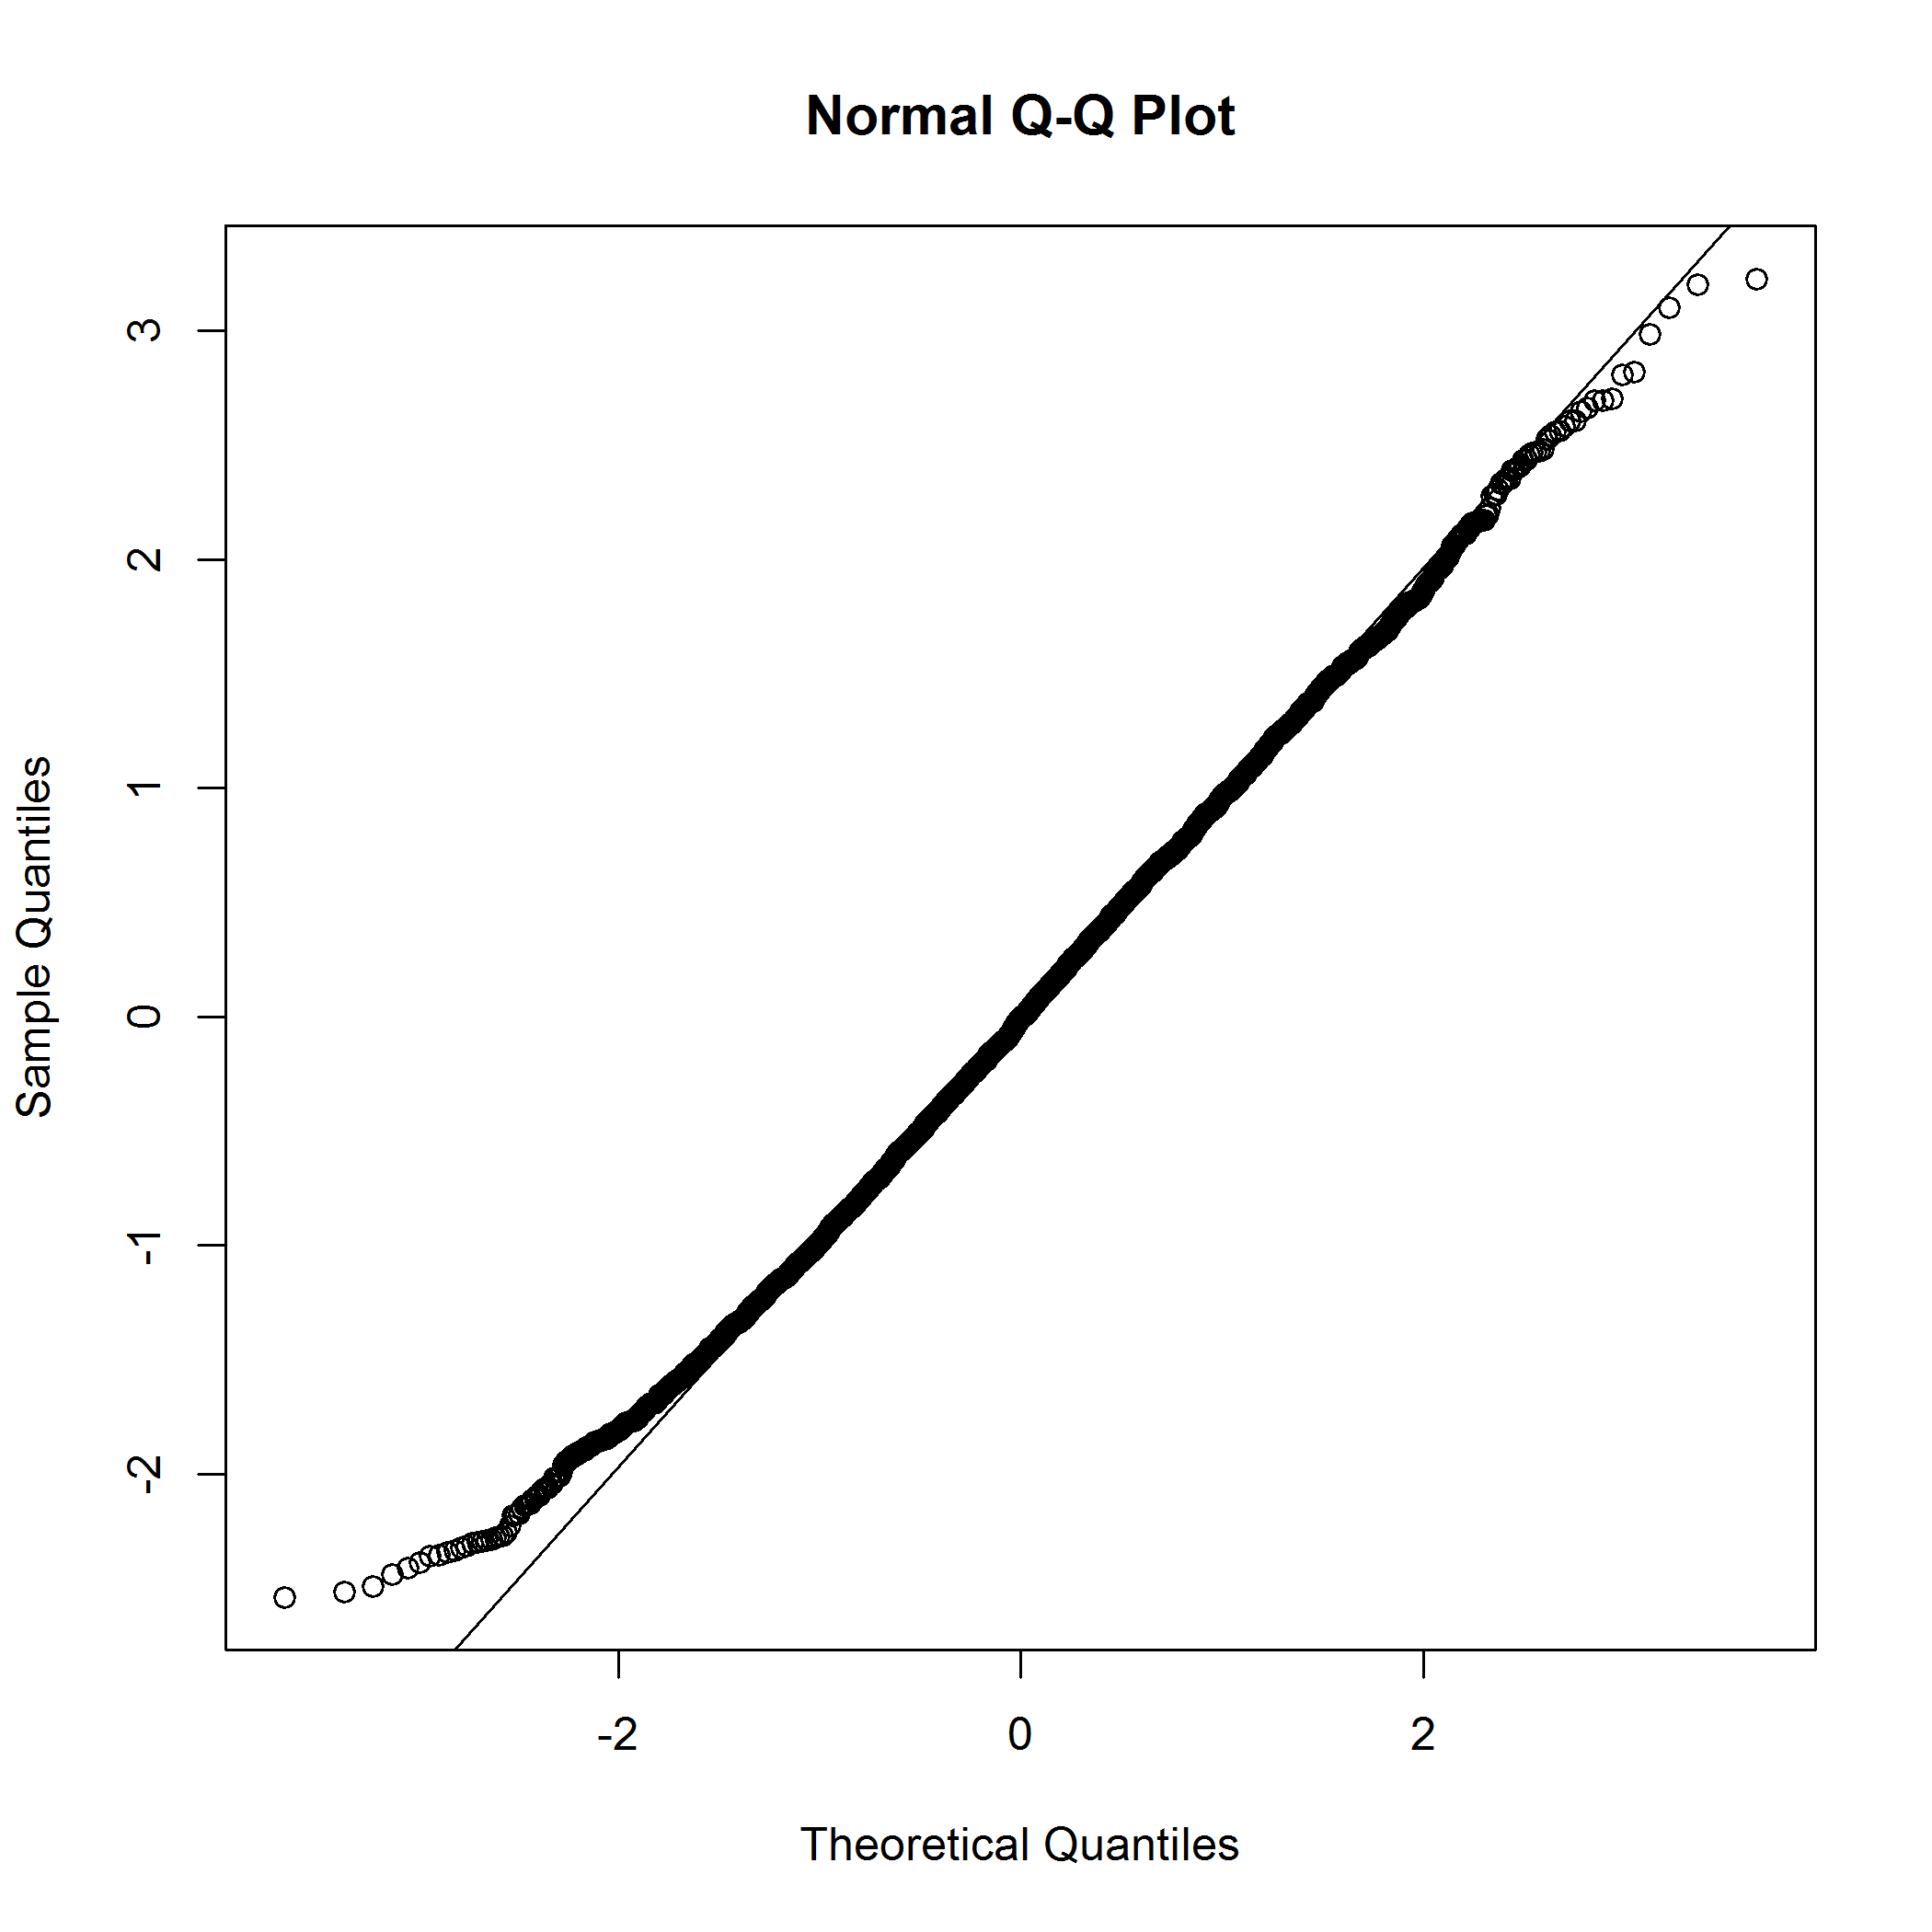
\includegraphics{Figures/Fleet12_RecPCOB_QQ.png}
\caption{Q-Q plot used to validate the goodness of fit of the lognormal
model for the CPFV onboard observer retained only catch.
\label{fig:Fleet12_RecPCOBR_QQ}}
\end{figure}

\begin{figure}[htbp]
\centering
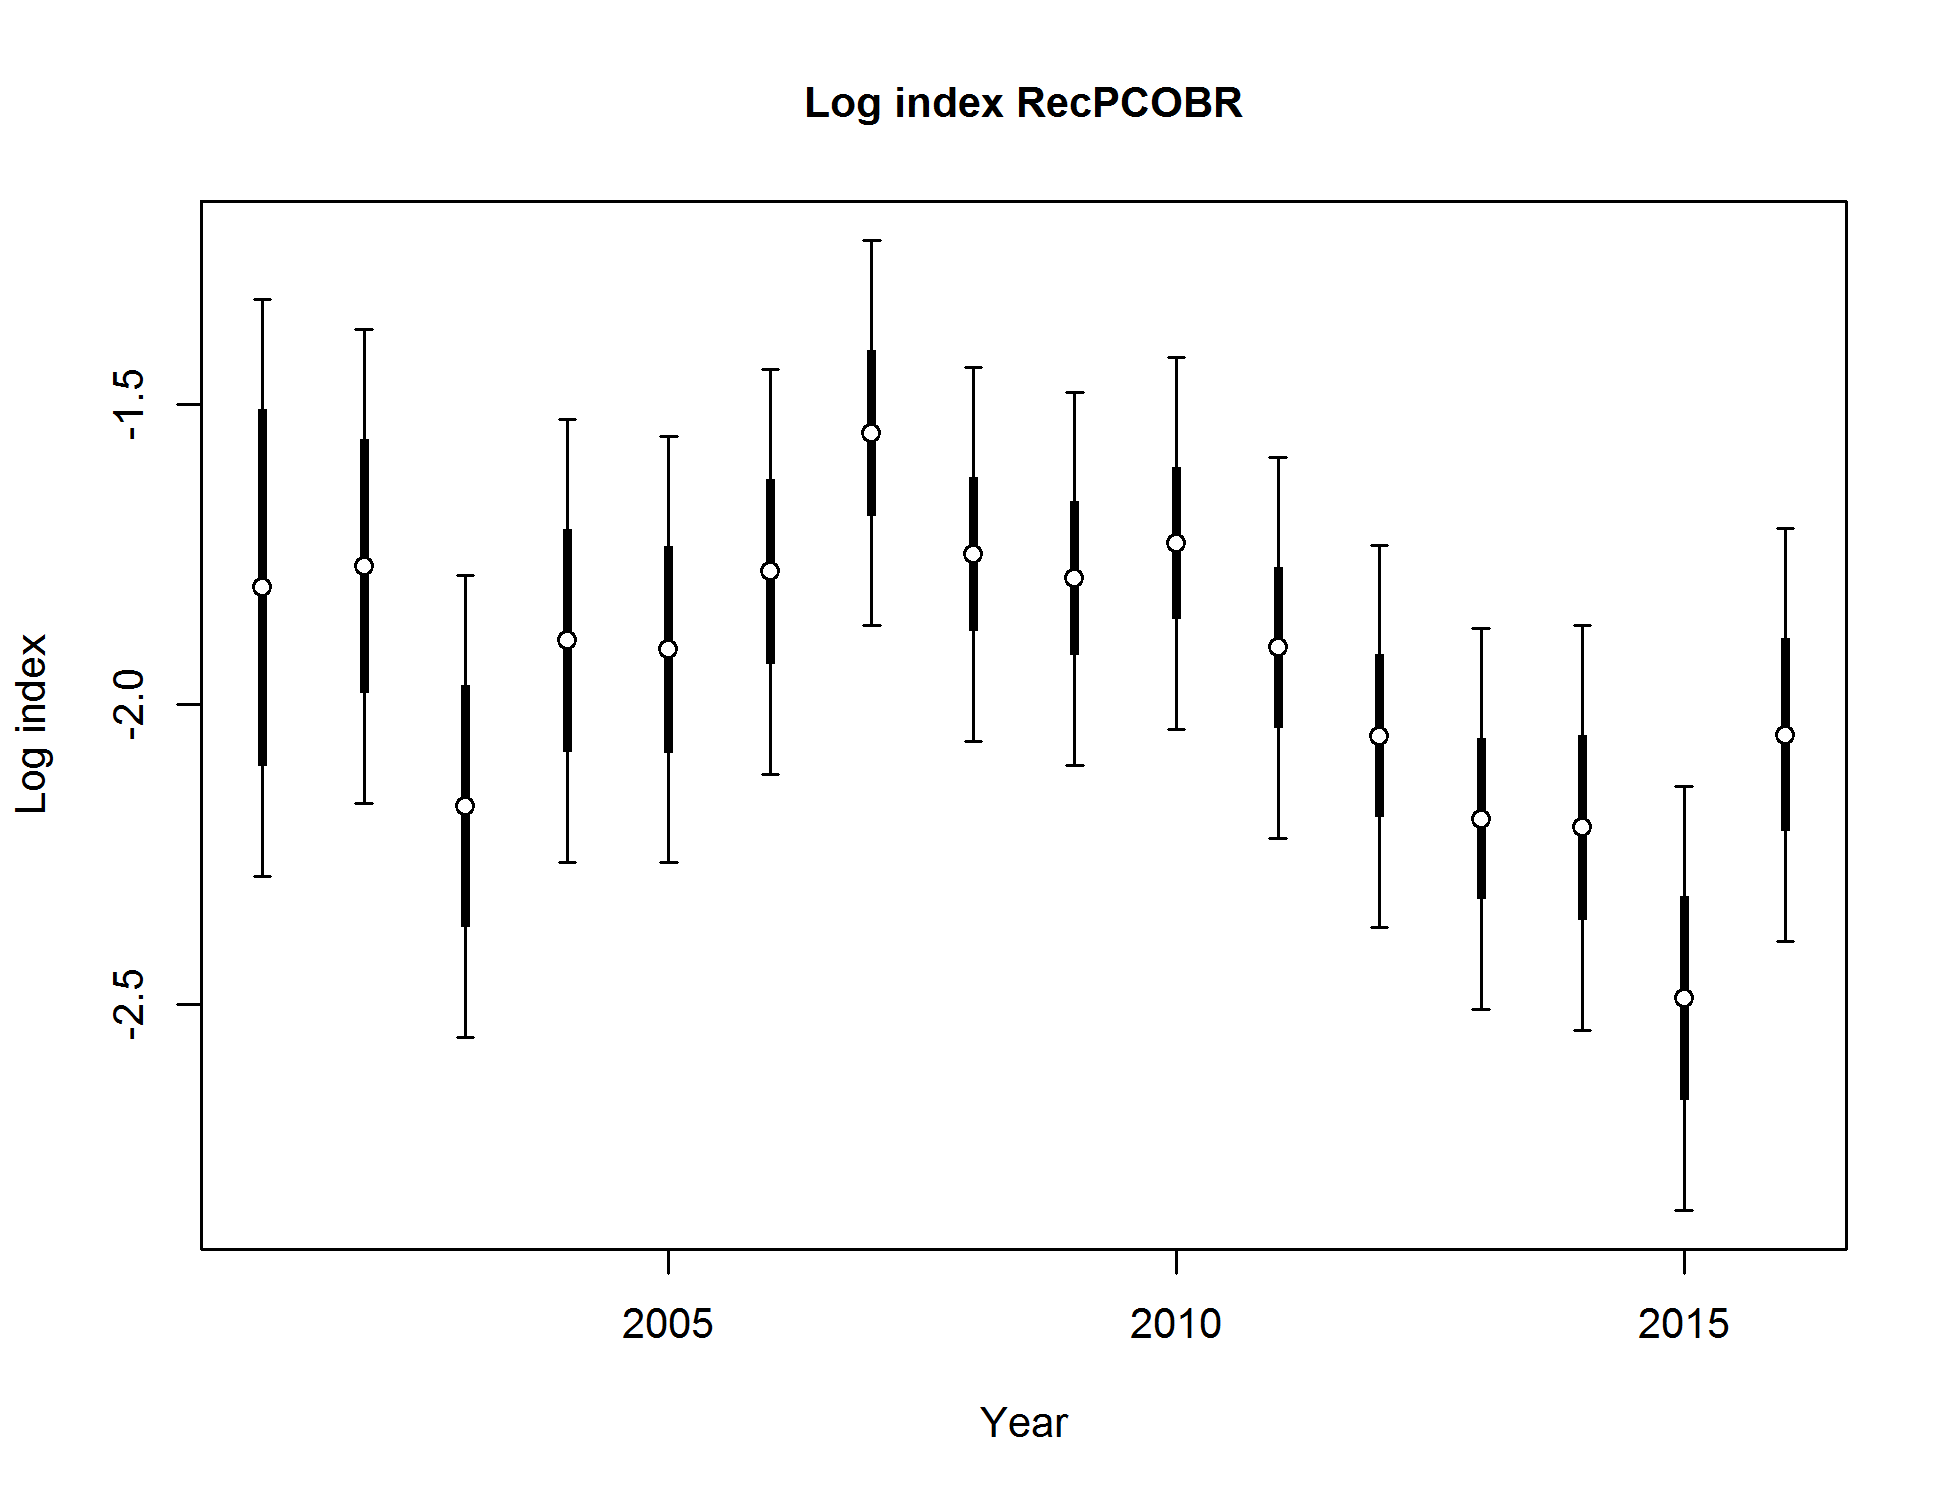
\includegraphics{r4ss/plots_mod1/index4_logcpuedata_RecPCOBR.png}
\caption{Standardized index on the log scale for the recreational CPFV
onboard observer retained catch index. Lines indicate 95\% uncertainty
interval around index values. Thicker lines indicate input uncertainty
before addition of estimated additional uncertainty parameter.
\label{fig:Fleet12_index4_logcpuedata_RecPCOBR}}
\end{figure}

\FloatBarrier

\begin{figure}[htbp]
\centering
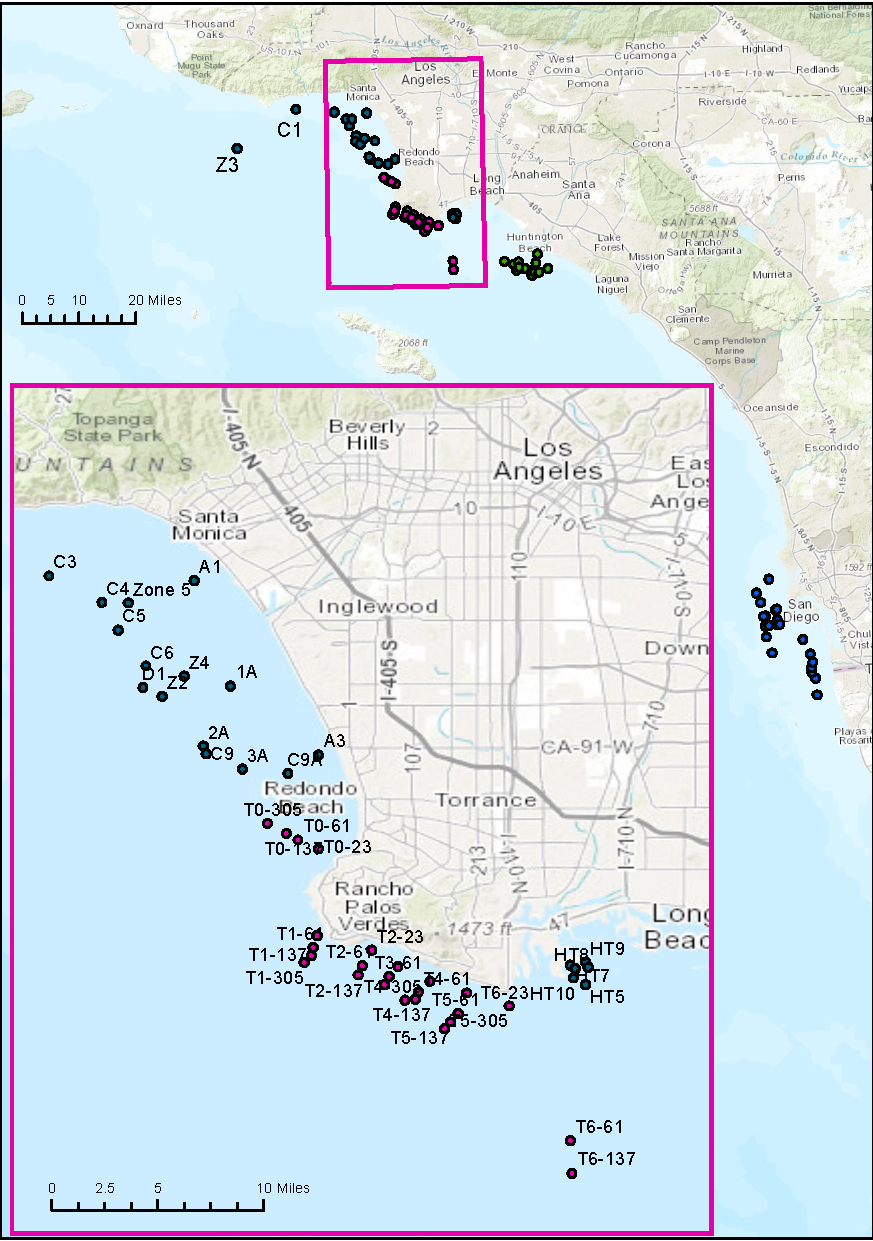
\includegraphics{Figures/Fleet7_sanitation_map2.pdf}
\caption{Map of stations sampled in at least 5 years by the Sanitation
Districts of Los Angeles County (magenta) and the City of Los Angeles
Environmental Monitoring Division (blue)
\label{fig:Fleet7_sanitation_map2}}
\end{figure}

\begin{figure}[htbp]
\centering
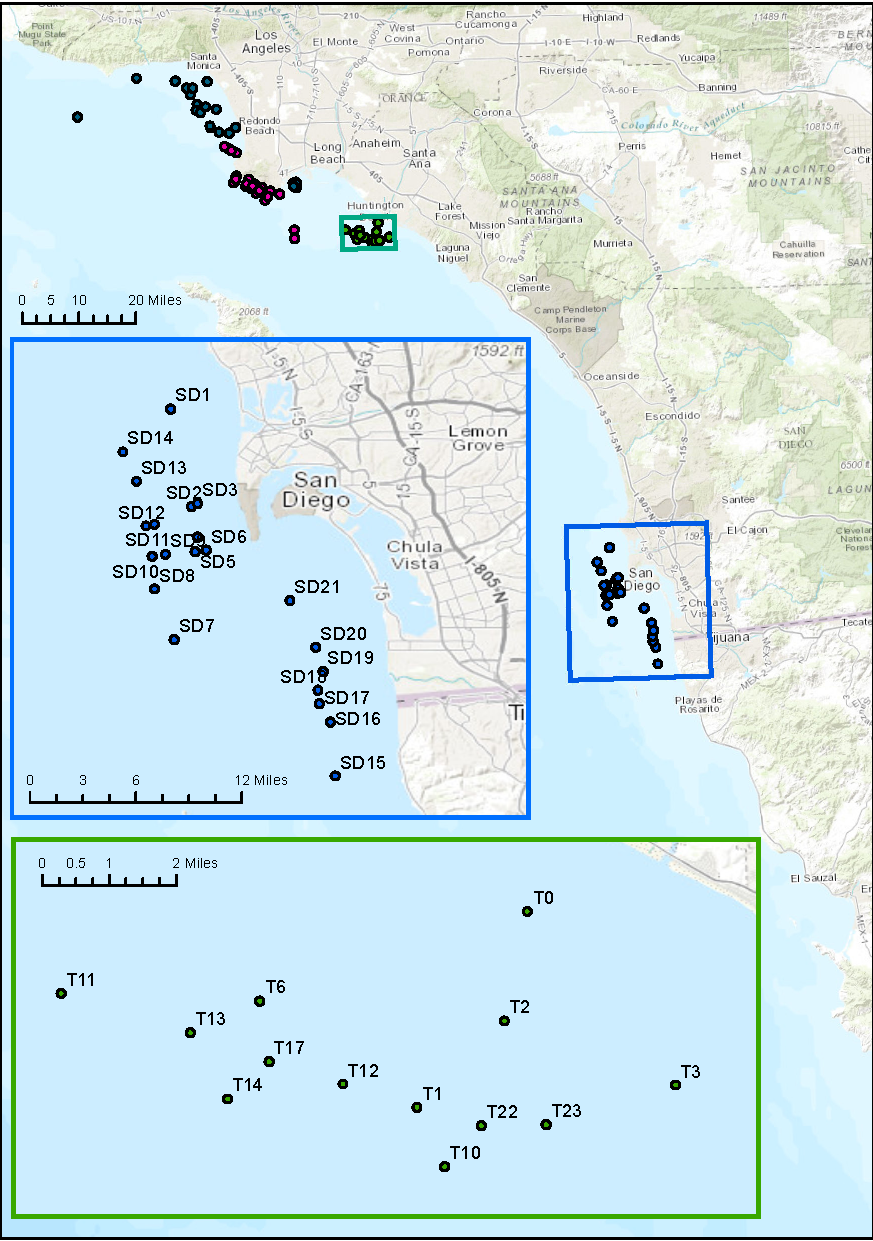
\includegraphics{Figures/Fleet7_sanitation_map1.pdf}
\caption{Map of stations sampled in at least 5 years by the Orange
County Sanitation District (green) and the City of San Diego Public
Utilities Ocean Monitoring Program (blue)
\label{fig:Fleet7_sanitation_map1}}
\end{figure}

\begin{figure}[htbp]
\centering
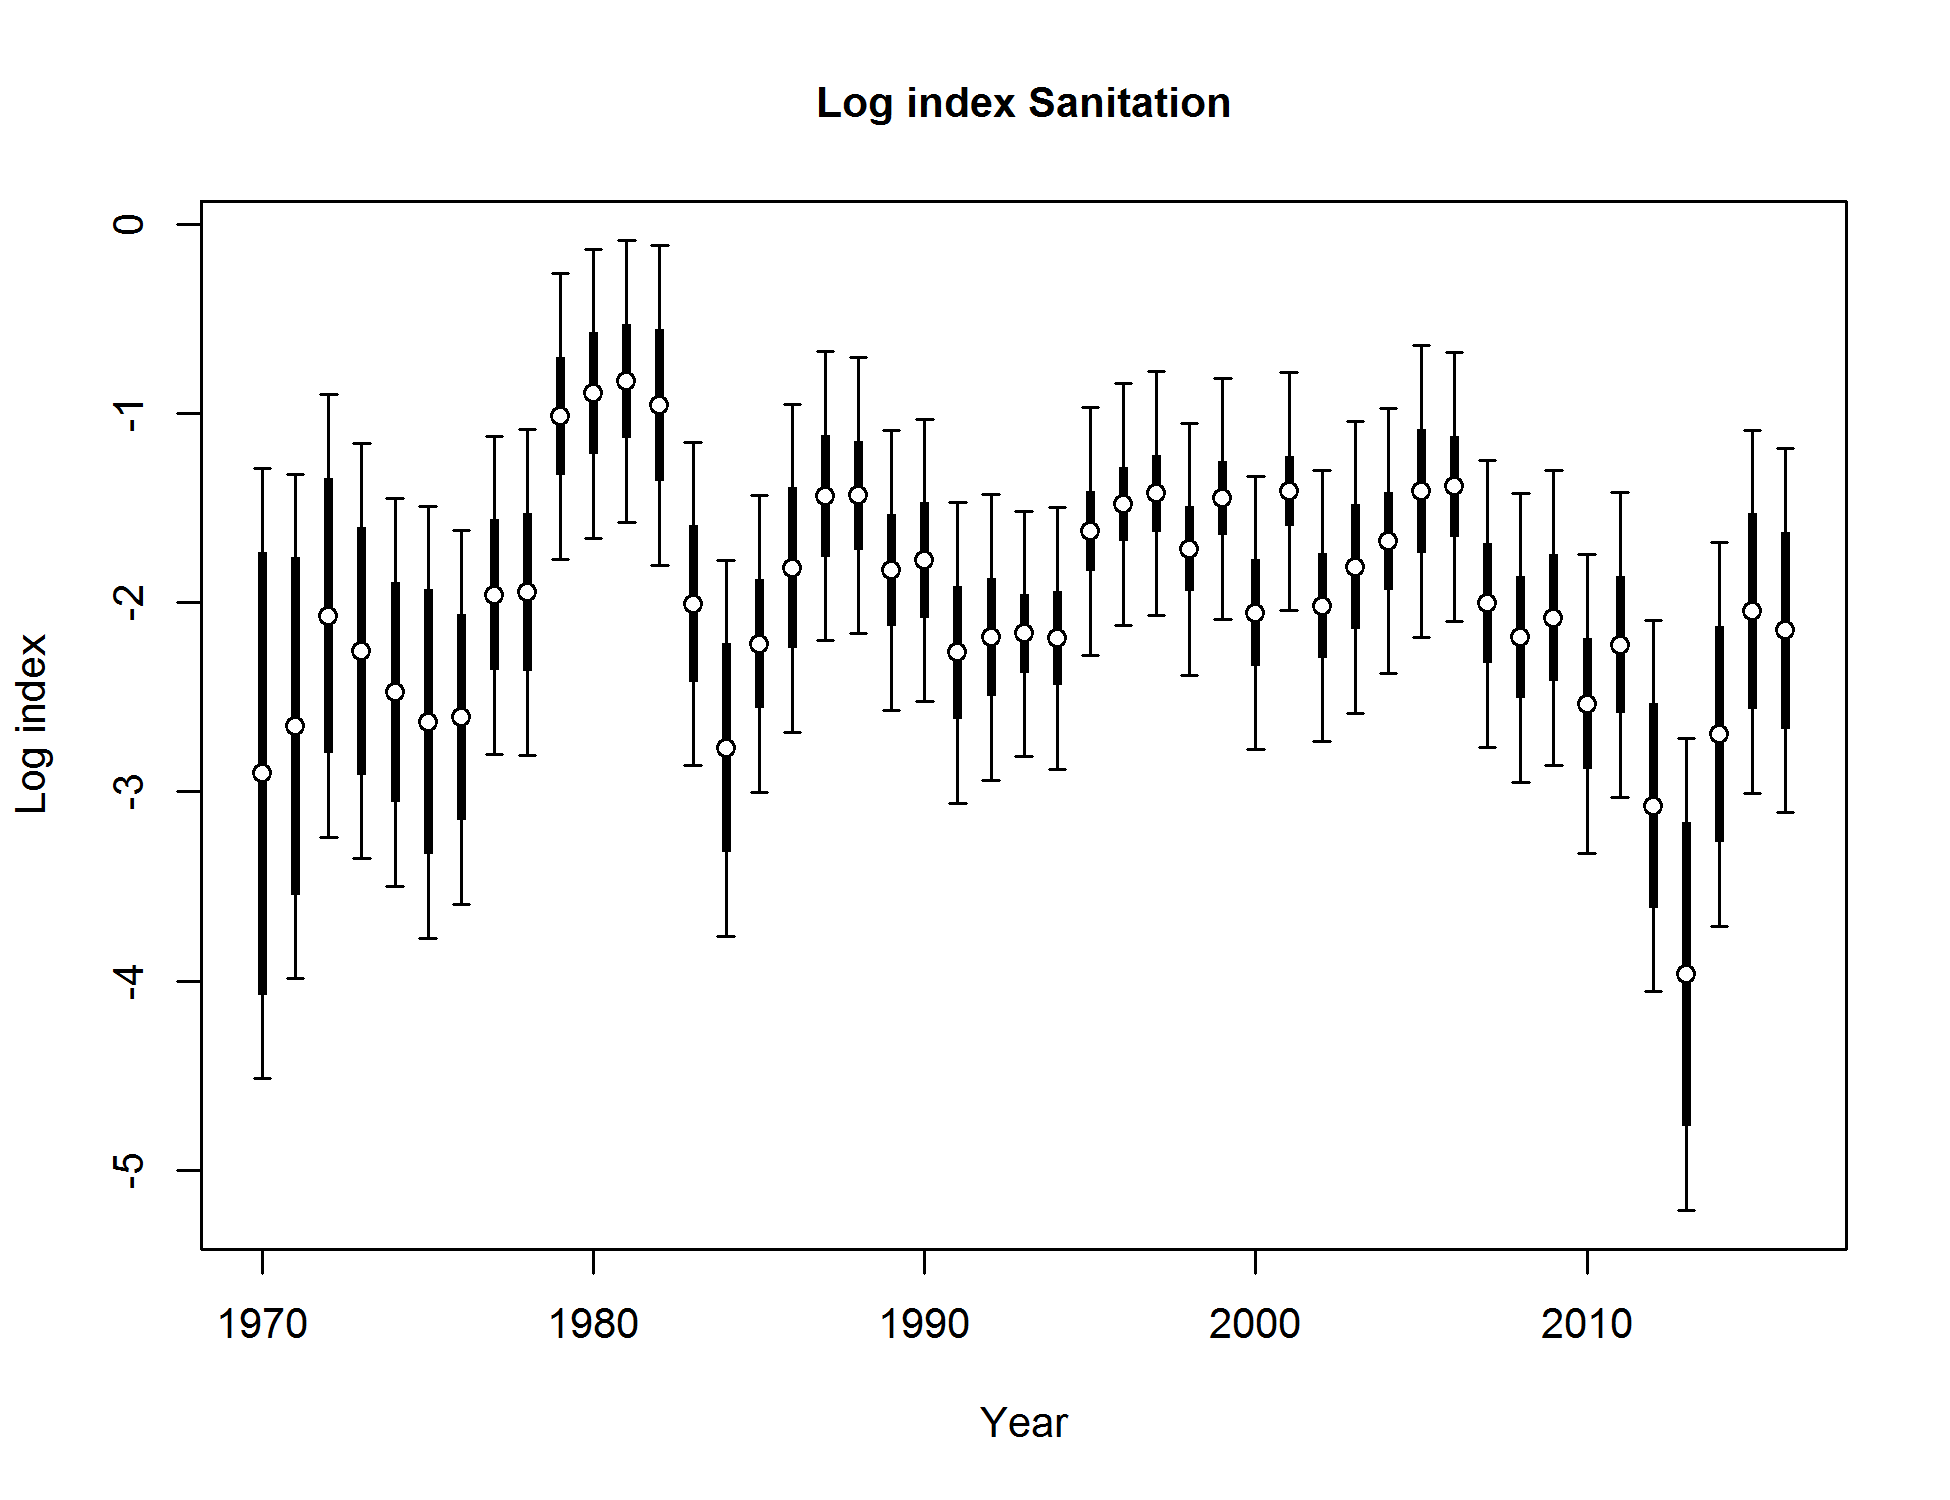
\includegraphics{r4ss/plots_mod1/index4_logcpuedata_Sanitation.png}
\caption{Standardized index on log scale for the Publicly Owned
Treatment Works monitoring programs trawl index. Lines indicate 95\%
uncertainty interval around index values. Thicker lines indicate input
uncertainty before addition of estimated additional uncertainty
parameter. \label{fig:index4_logcpuedata_Sanitation}}
\end{figure}

\begin{figure}[htbp]
\centering
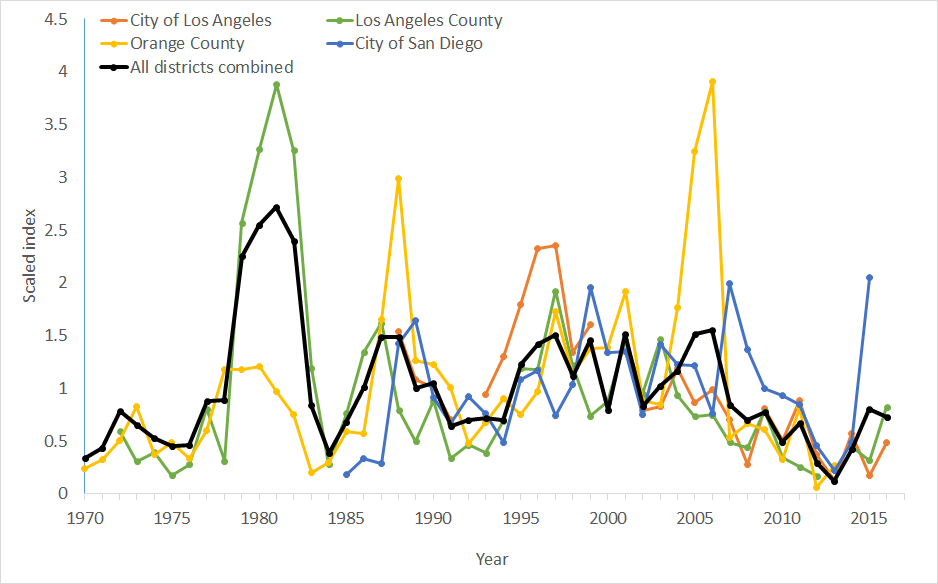
\includegraphics{Figures/Fleet7_Sanitation_indexcompare.png}
\caption{Comparison of standardized indices for each Publicly Owned
Treatment Works monitoring program independently and with data from all
Publicly Owned Treatment Works programs combined.
\label{fig:Fleet7_Sanitation_indexcompare}}
\end{figure}

\begin{figure}[htbp]
\centering
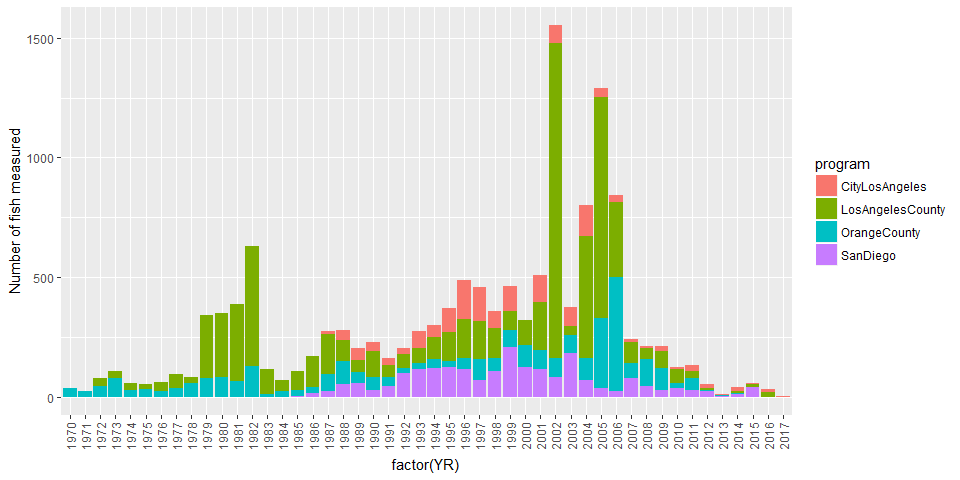
\includegraphics{Figures/Fleet7_Sanitation_length_source.png}
\caption{Sample sizes of measured California scorpionfish by Publicly
Owned Treatment Works monitoring program and year.
\label{fig:Fleet7_Sanitation_lengthbydistrict}}
\end{figure}

\begin{figure}[htbp]
\centering
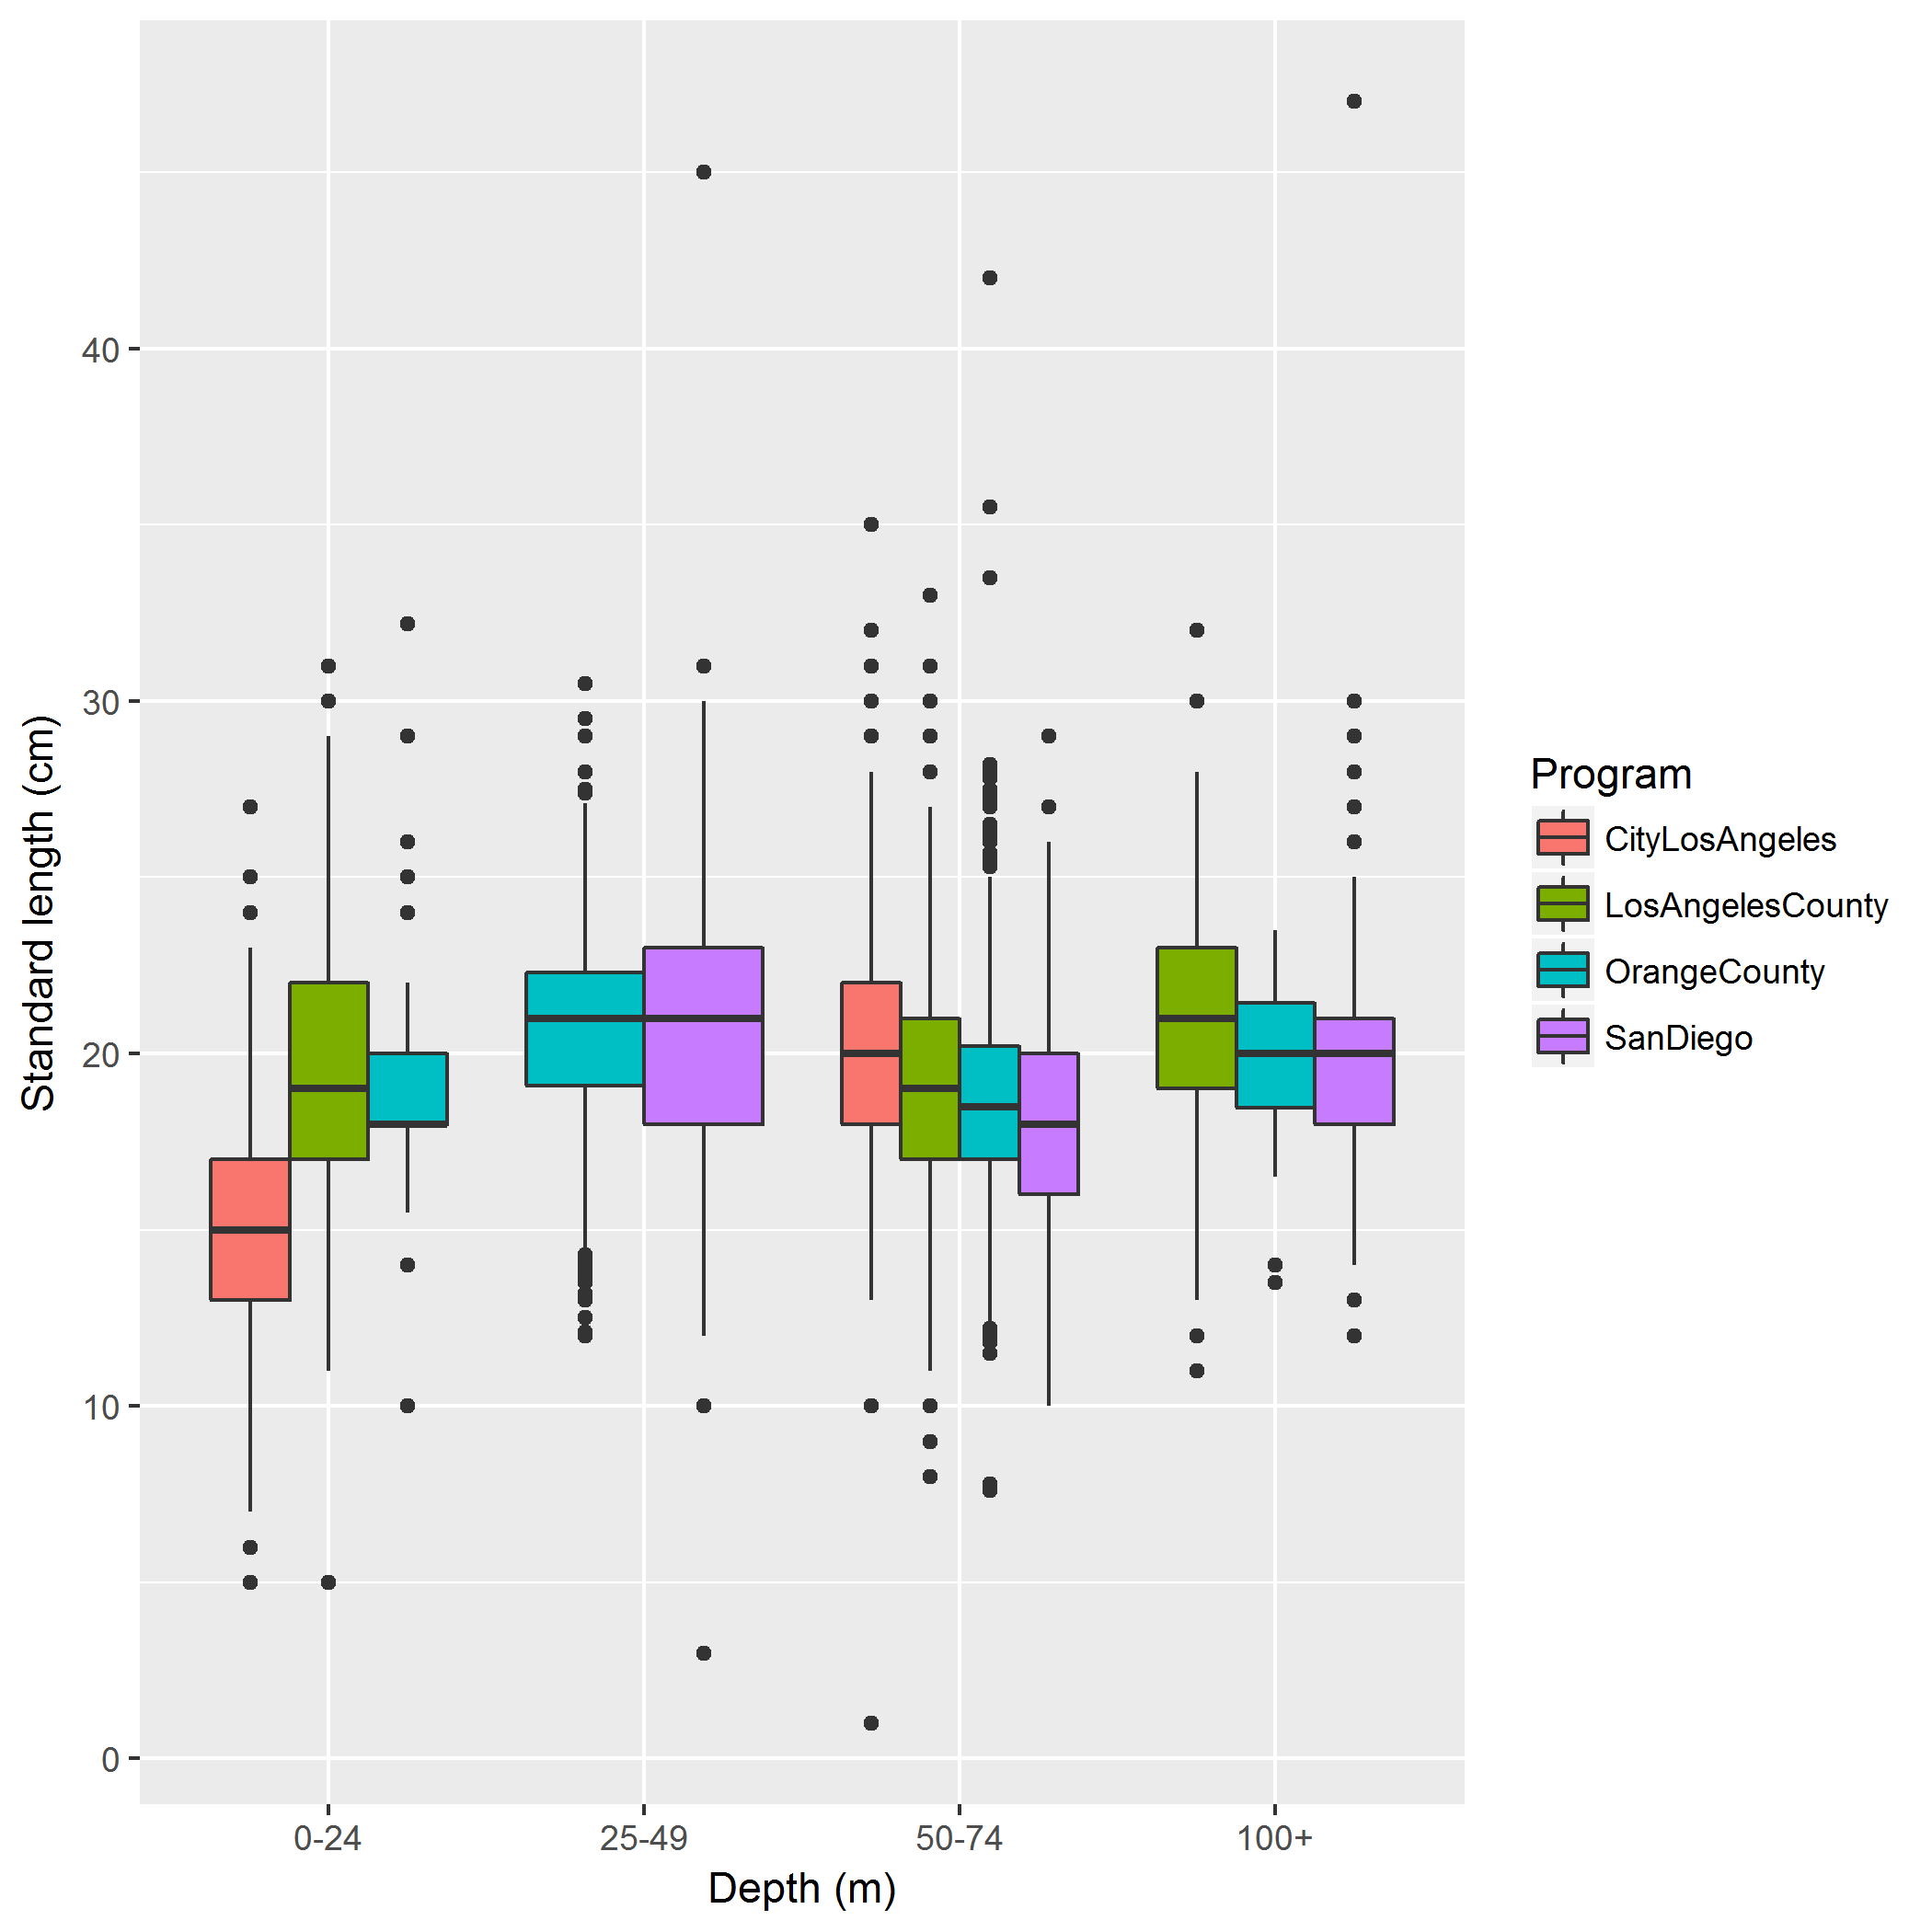
\includegraphics{Figures/Fleet7_Sanitation_lengthboxplots.png}
\caption{Boxplots of measured California scorpionfish from the Publicly
Owned Treatment Works monitoring surveys by program and 25 m depth bins.
\label{fig:Fleet7_Sanitation_lengthboxplots}}
\end{figure}

\FloatBarrier

\begin{figure}[htbp]
\centering
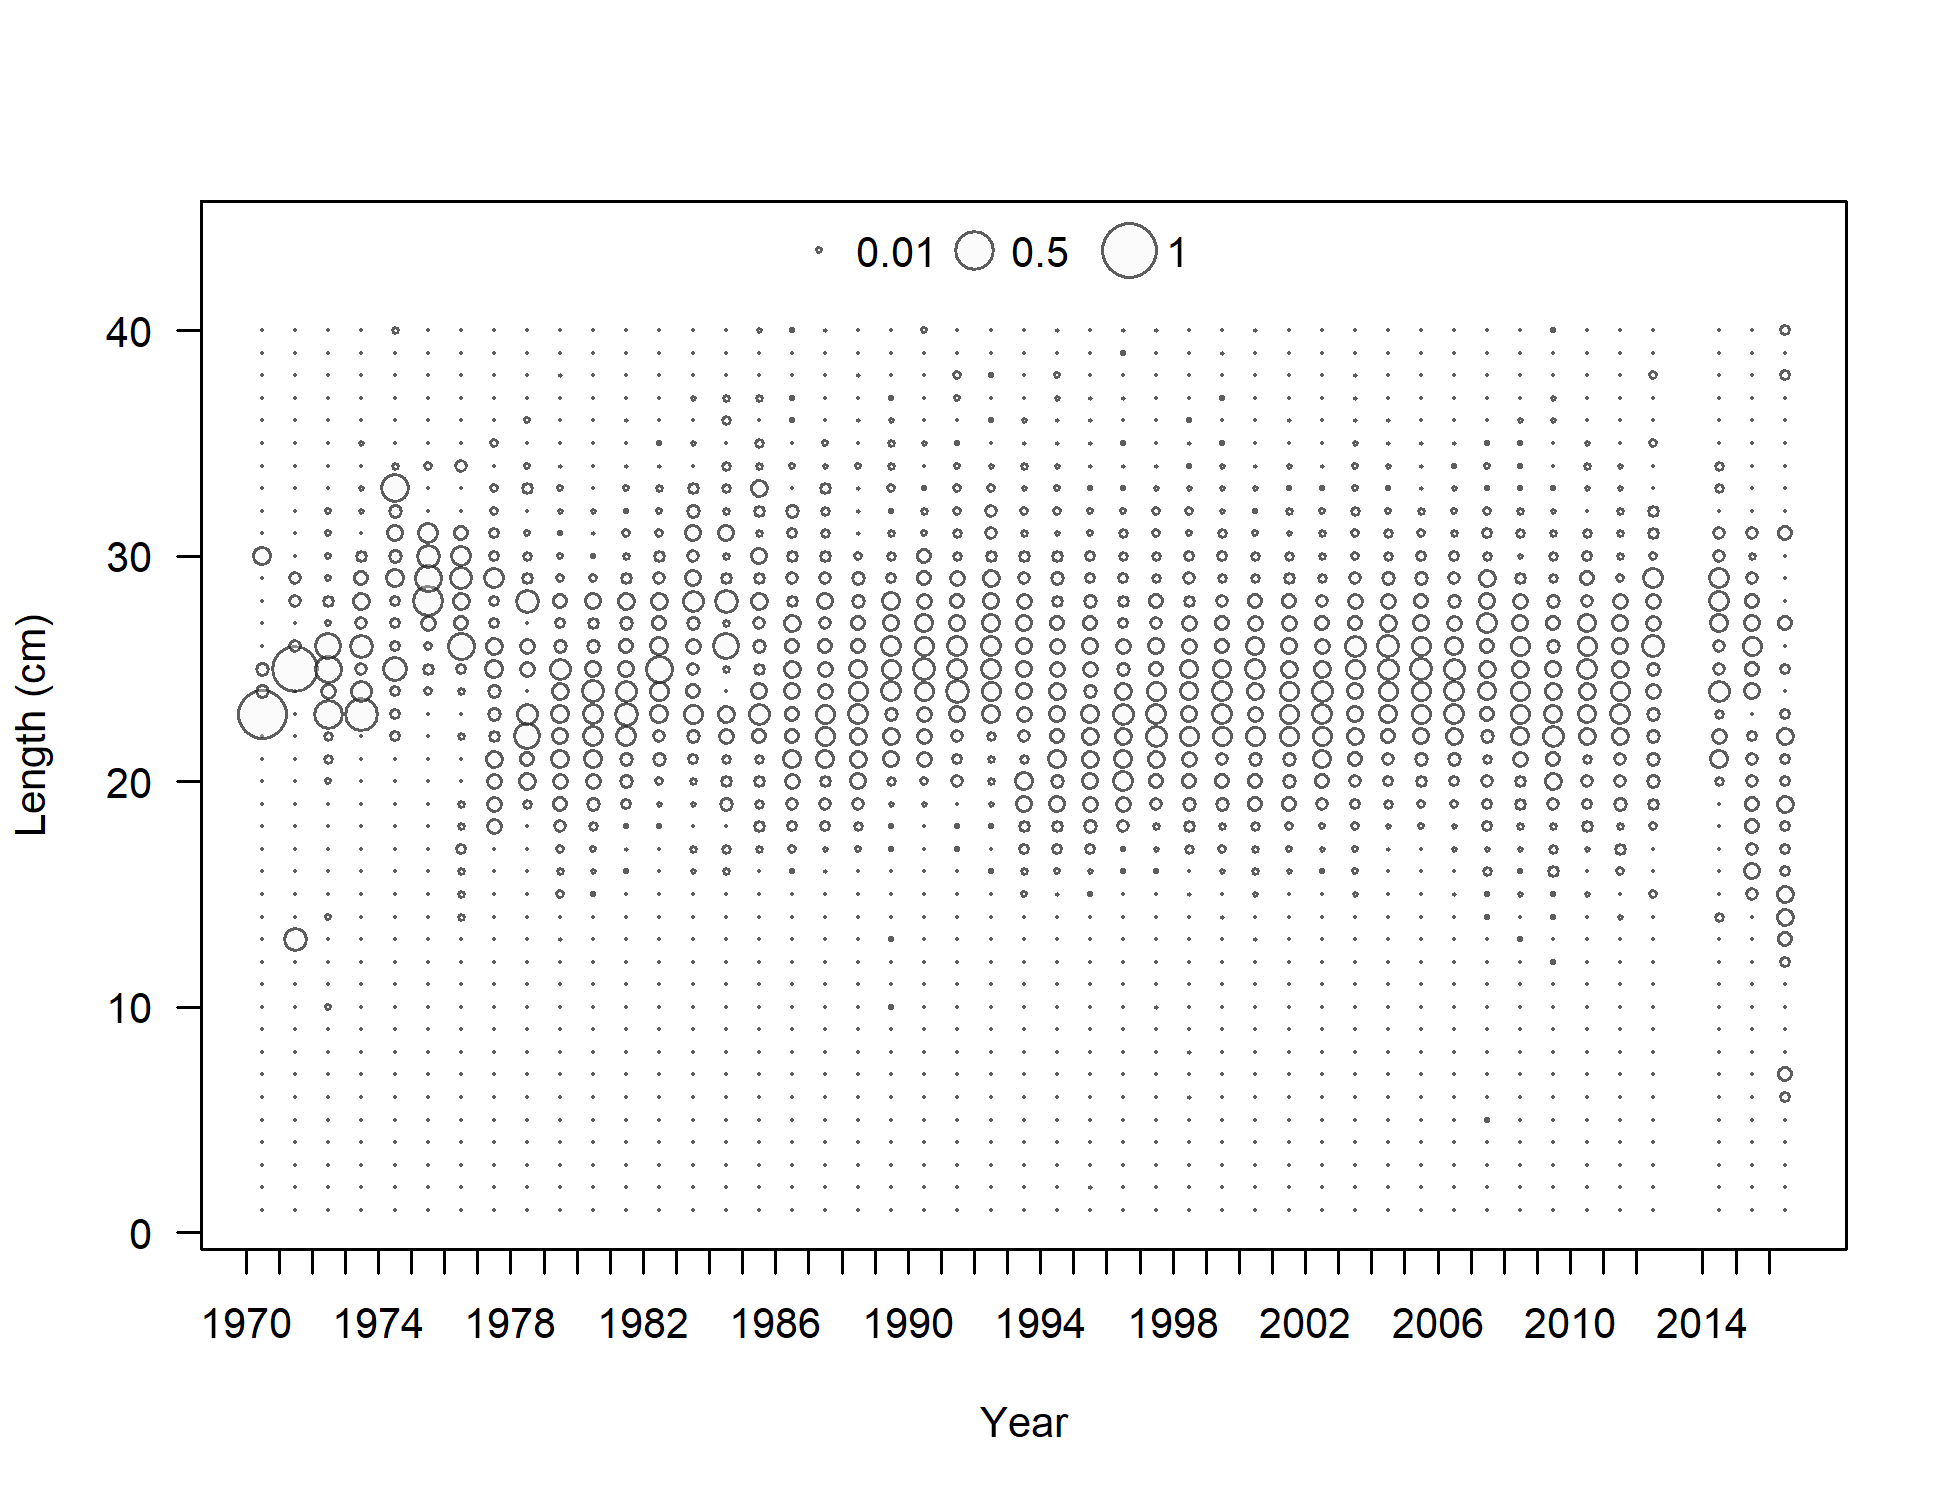
\includegraphics{r4ss/plots_mod1/comp_lendat_bubflt7mkt2_page2.png}
\caption{Length frequency distributions from the Publicly Owned
Treatment Works monitoring trawl surveys.
\label{fig:Fleet7_comp_lendat_bubflt10mkt2}}
\end{figure}

\FloatBarrier

\begin{figure}[htbp]
\centering
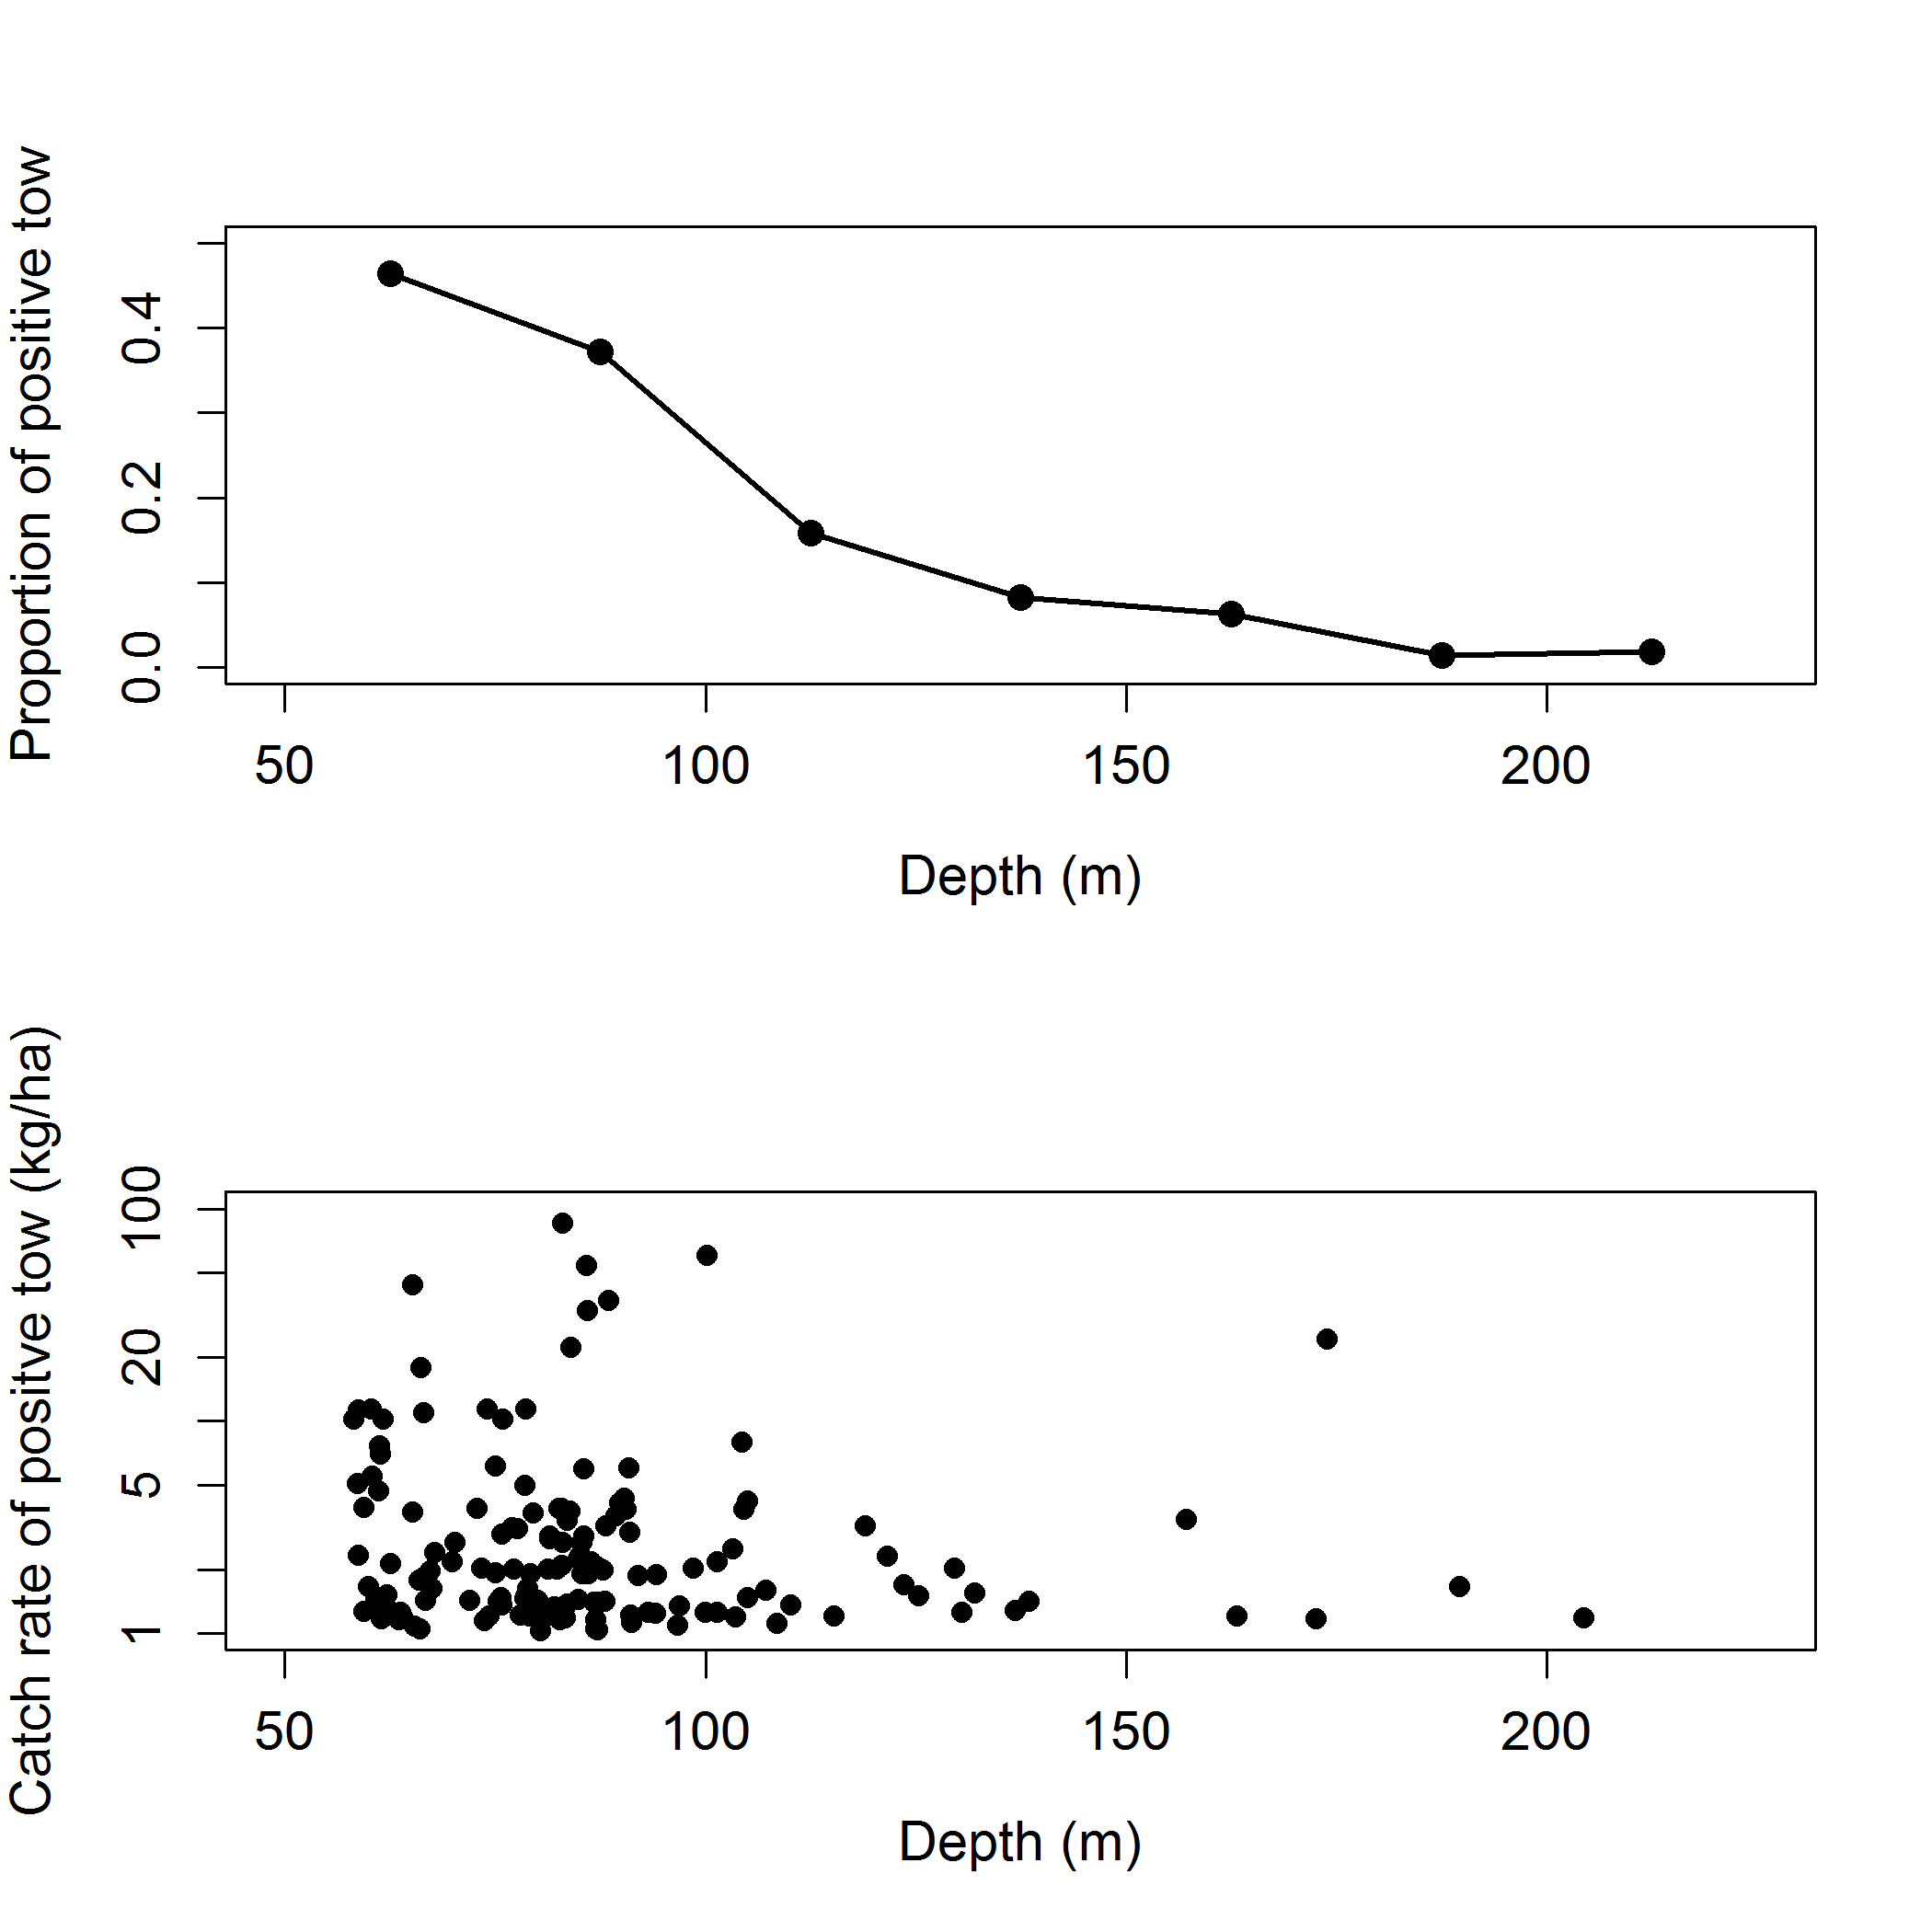
\includegraphics{Figures/NWFSCtrawl_posdepth.png}
\caption{Plots of the proportion of positive tows (top panel) and the
raw catch rates of positive tows (bottom panel) by depth zones (25 m
interval) for NWFSC trawl survey.
\label{fig:Fleet8_NWFSCtrawl_posdepth}}
\end{figure}

\FloatBarrier

\begin{figure}[htbp]
\centering
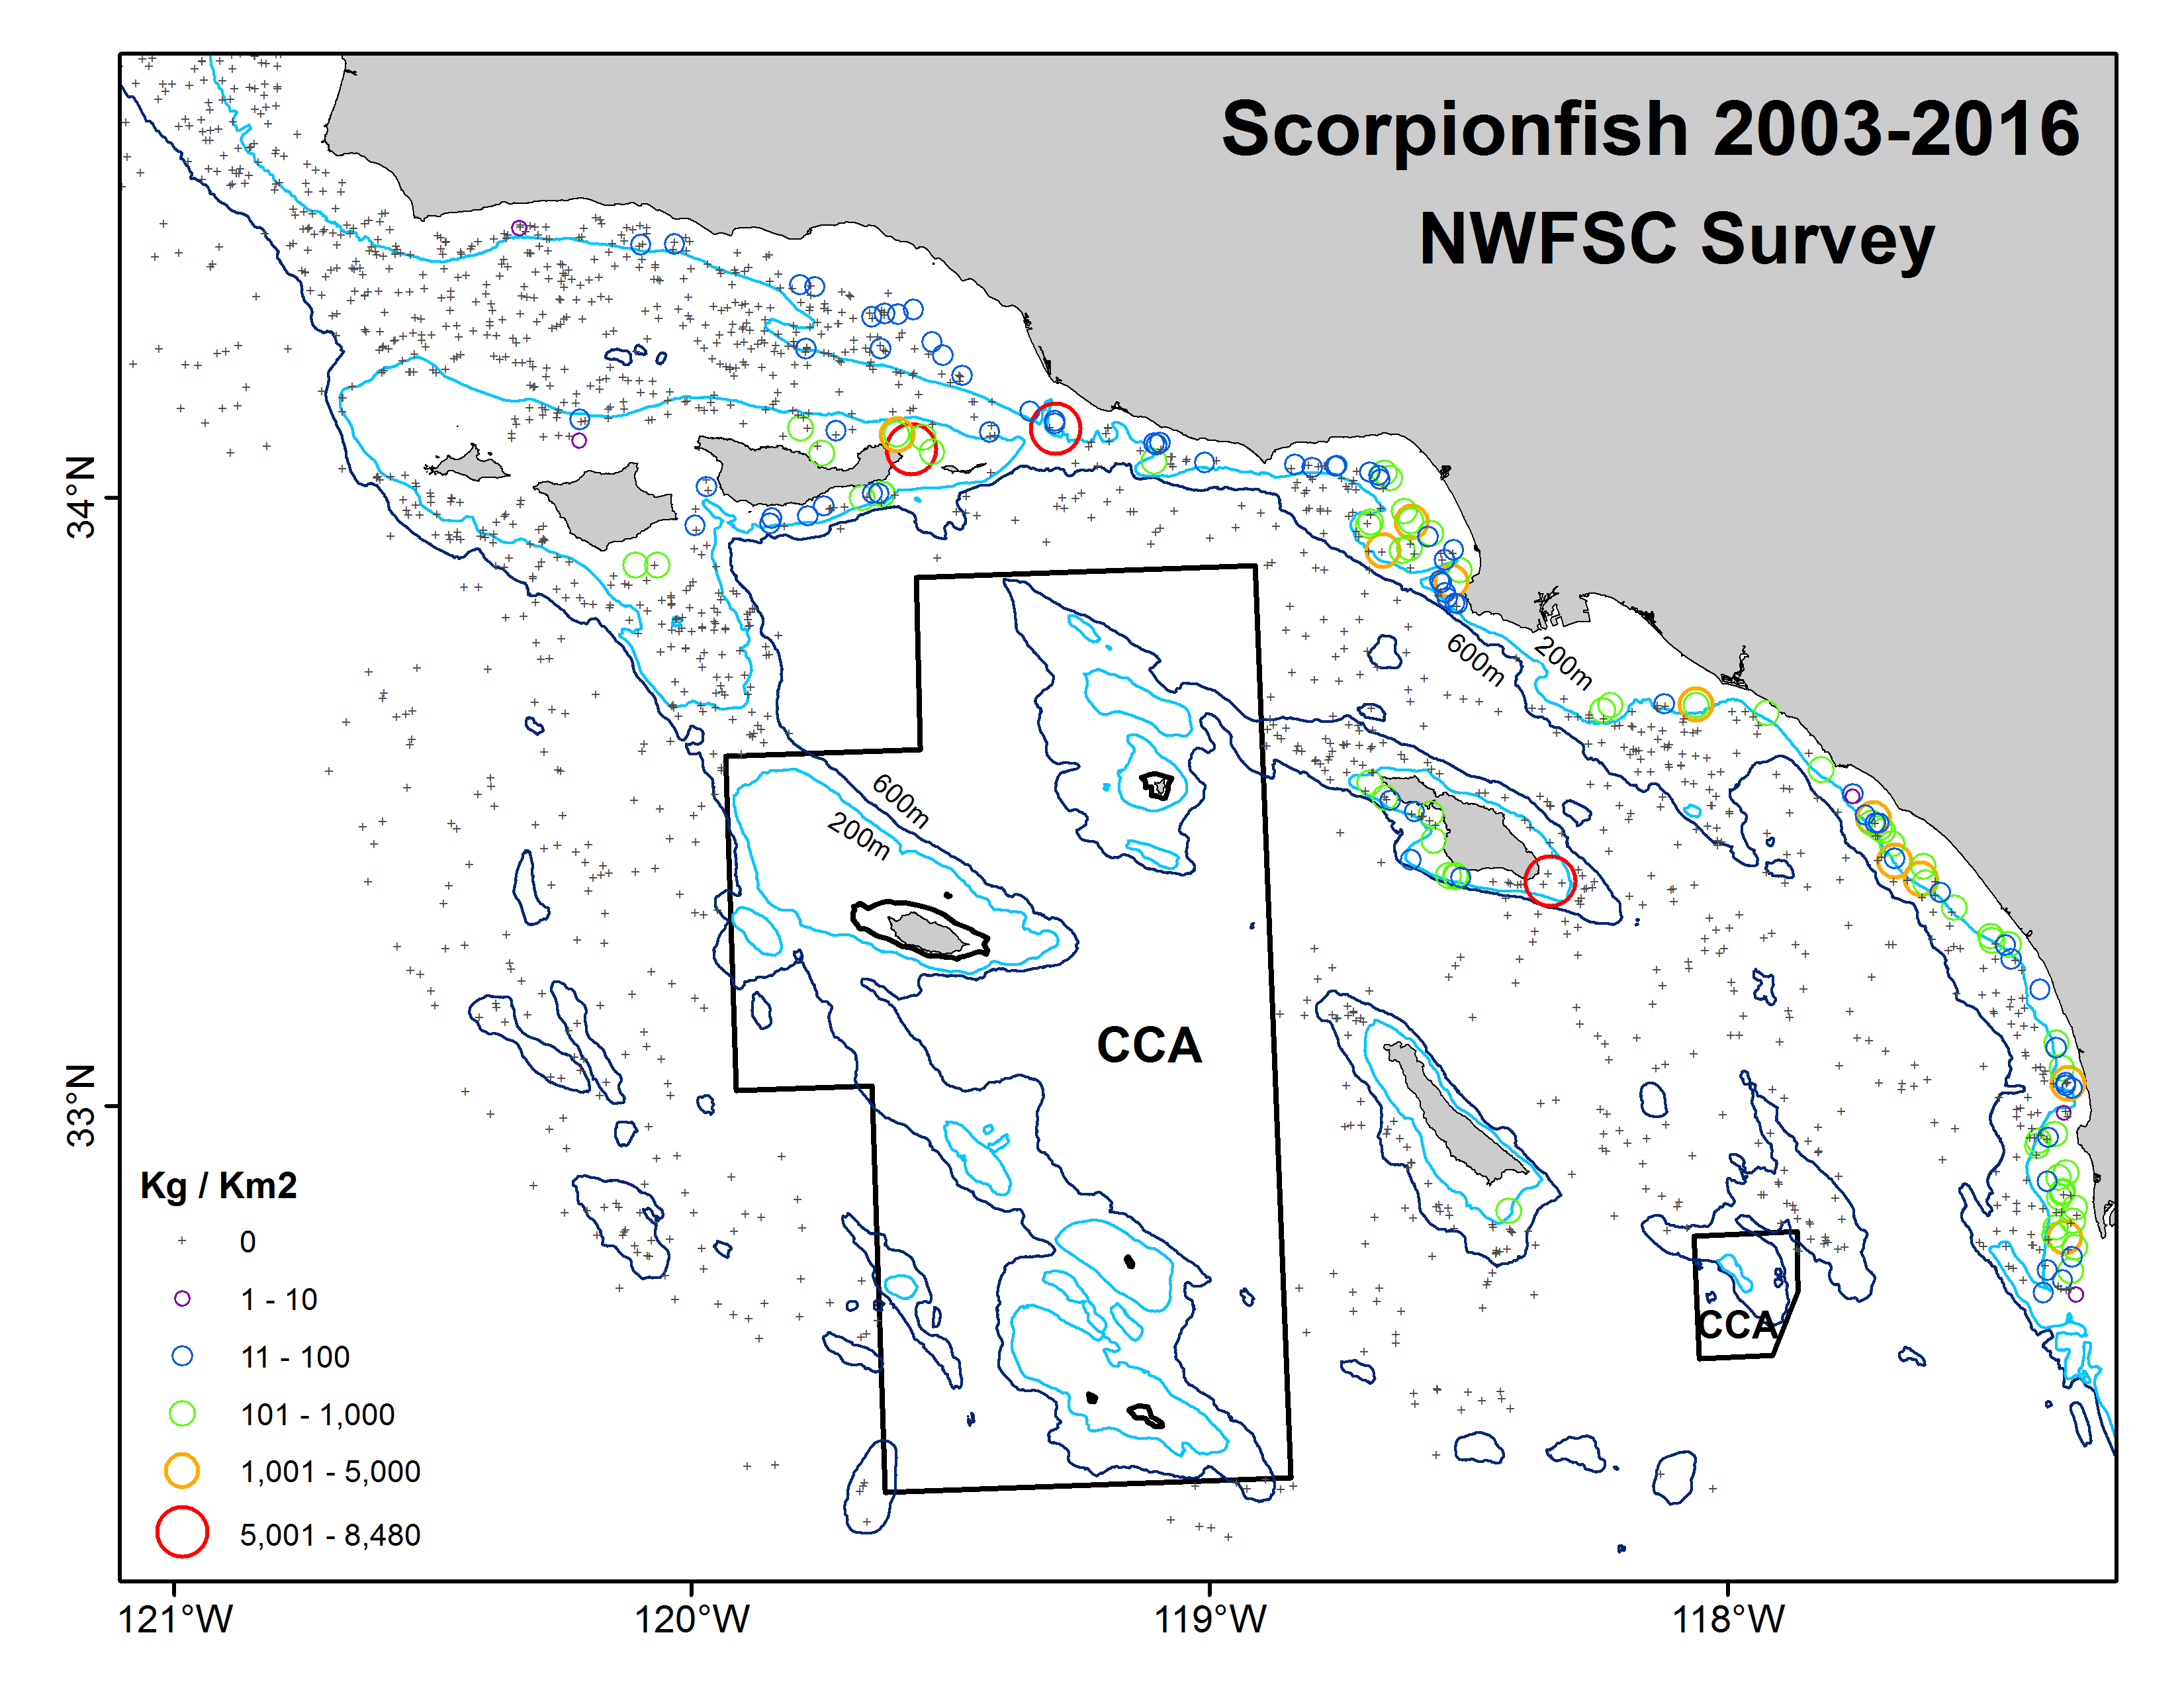
\includegraphics{Figures/NWFSCtrawl_map.png}
\caption{Spatial distribution of raw catch rates of Scorpionfish from
NWFSC trawl survey between 2003 and 2016. Depth contour lines of 200 m
and 600 m and the CCA areas are shown. Note that sizes and colors of
circles represent catch rate in log scales (Credit of Rebecca Miller,
SWFSC). \label{fig:Fleet8_NWFSCtrawl_map}}
\end{figure}

\begin{figure}[htbp]
\centering
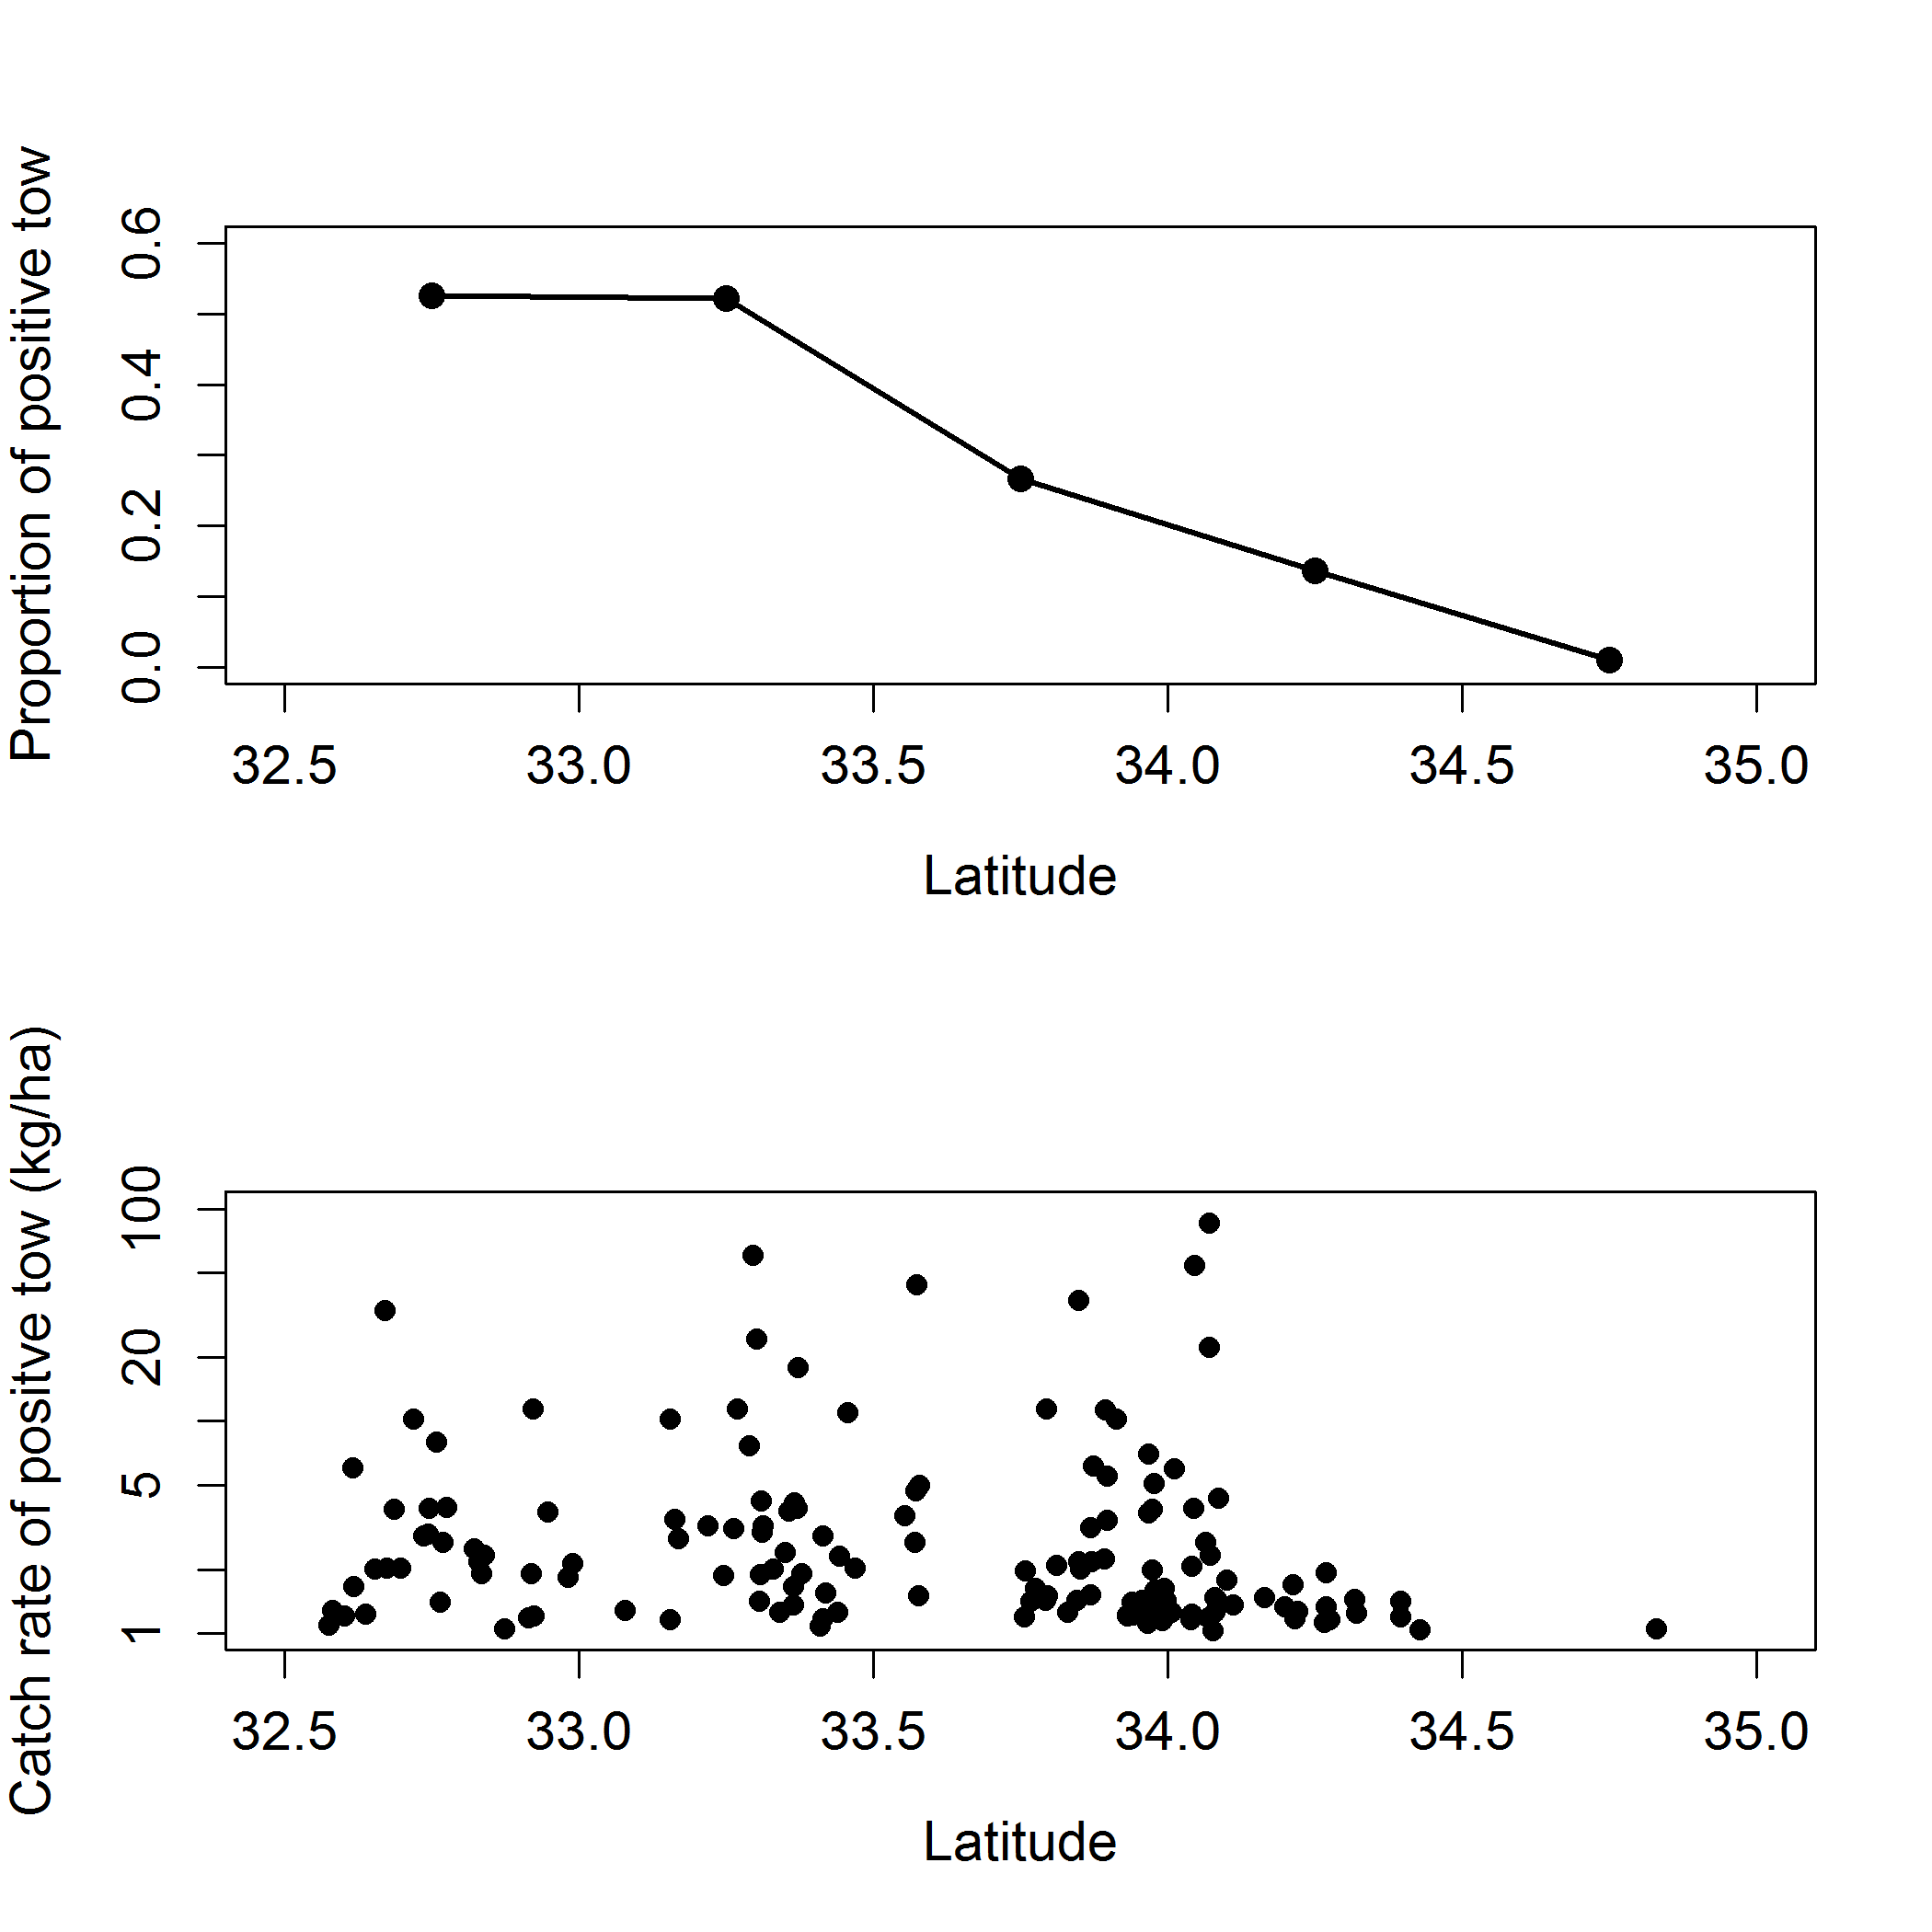
\includegraphics{Figures/NWFSCtrawl_poslat.png}
\caption{Plots of the proportion of positive tows (top panel) and the
raw catch rates of positive tows (bottom panel) by latitude zones (0.5
degree interval) for NWFSC trawl survey.
\label{fig:Fleet8_NWFSCtrawl_poslat}}
\end{figure}

\FloatBarrier

\begin{figure}[htbp]
\centering
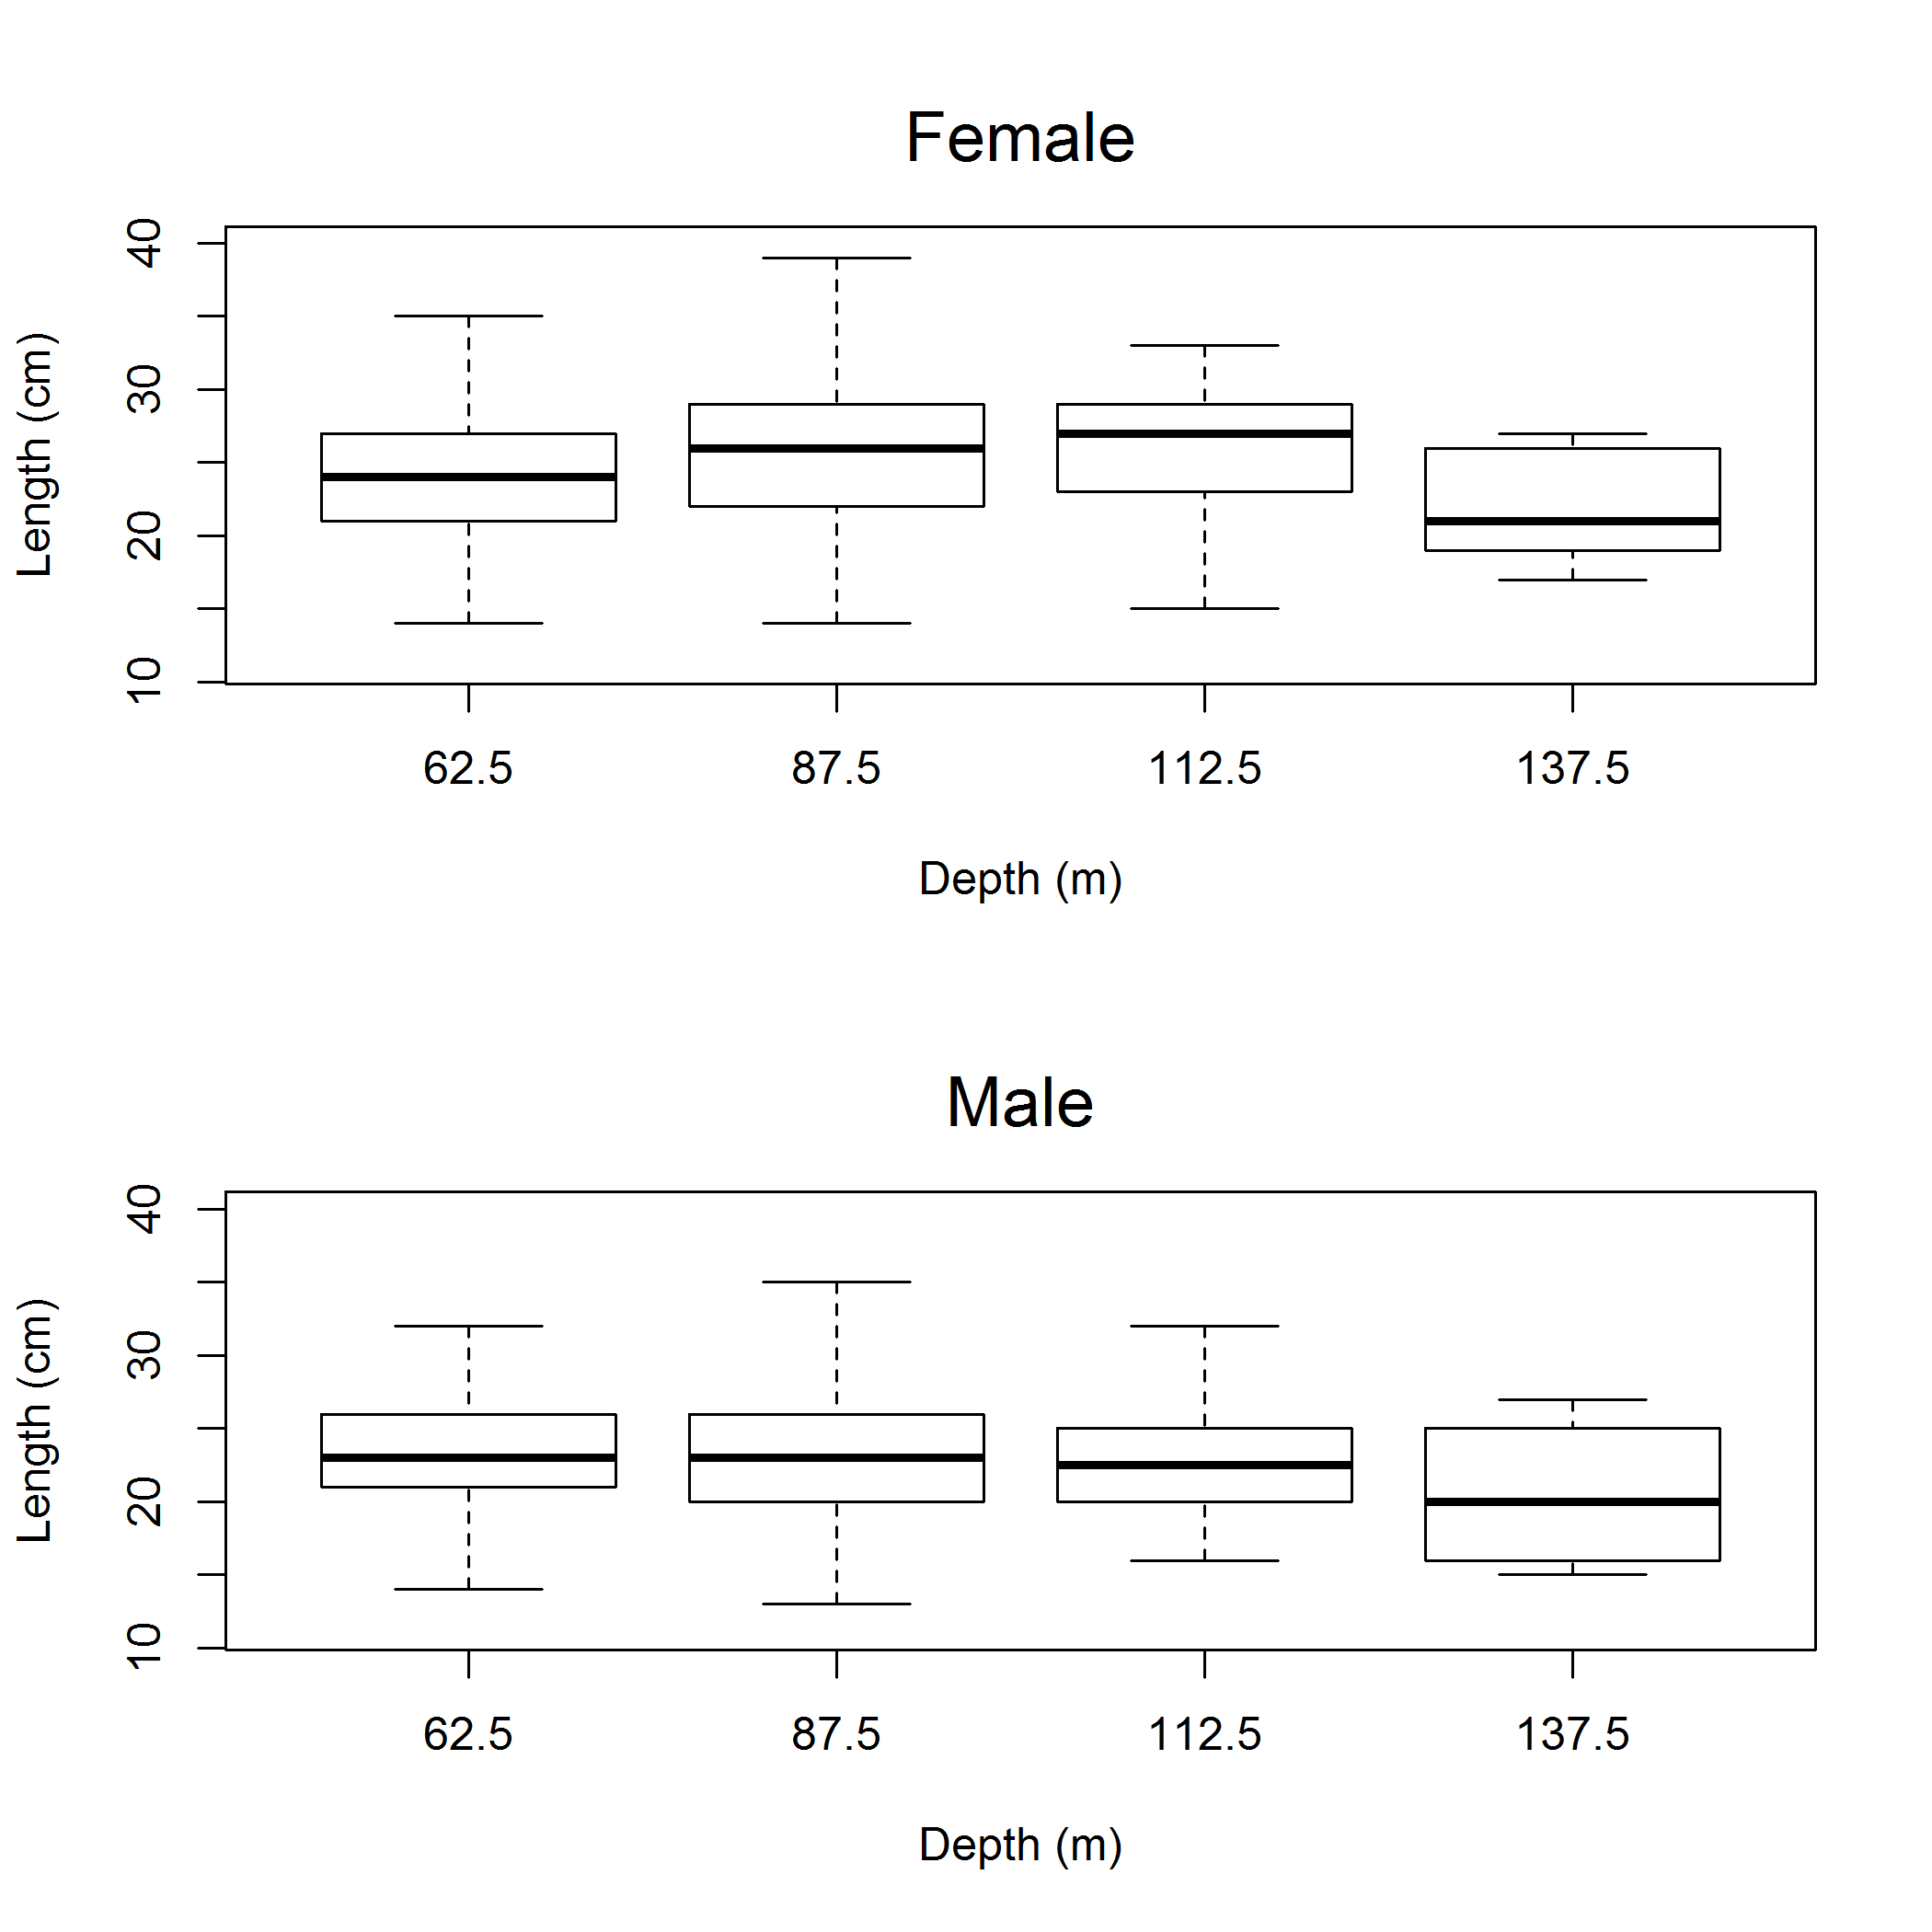
\includegraphics{Figures/NWFSCtrawl_lengthdepth.png}
\caption{Comparison box plots of raw length data from NWFSC trawl survey
by depth zone and sex. \label{fig:Fleet8_NWFSCtrawl_lengthdepth}}
\end{figure}

\begin{figure}[htbp]
\centering
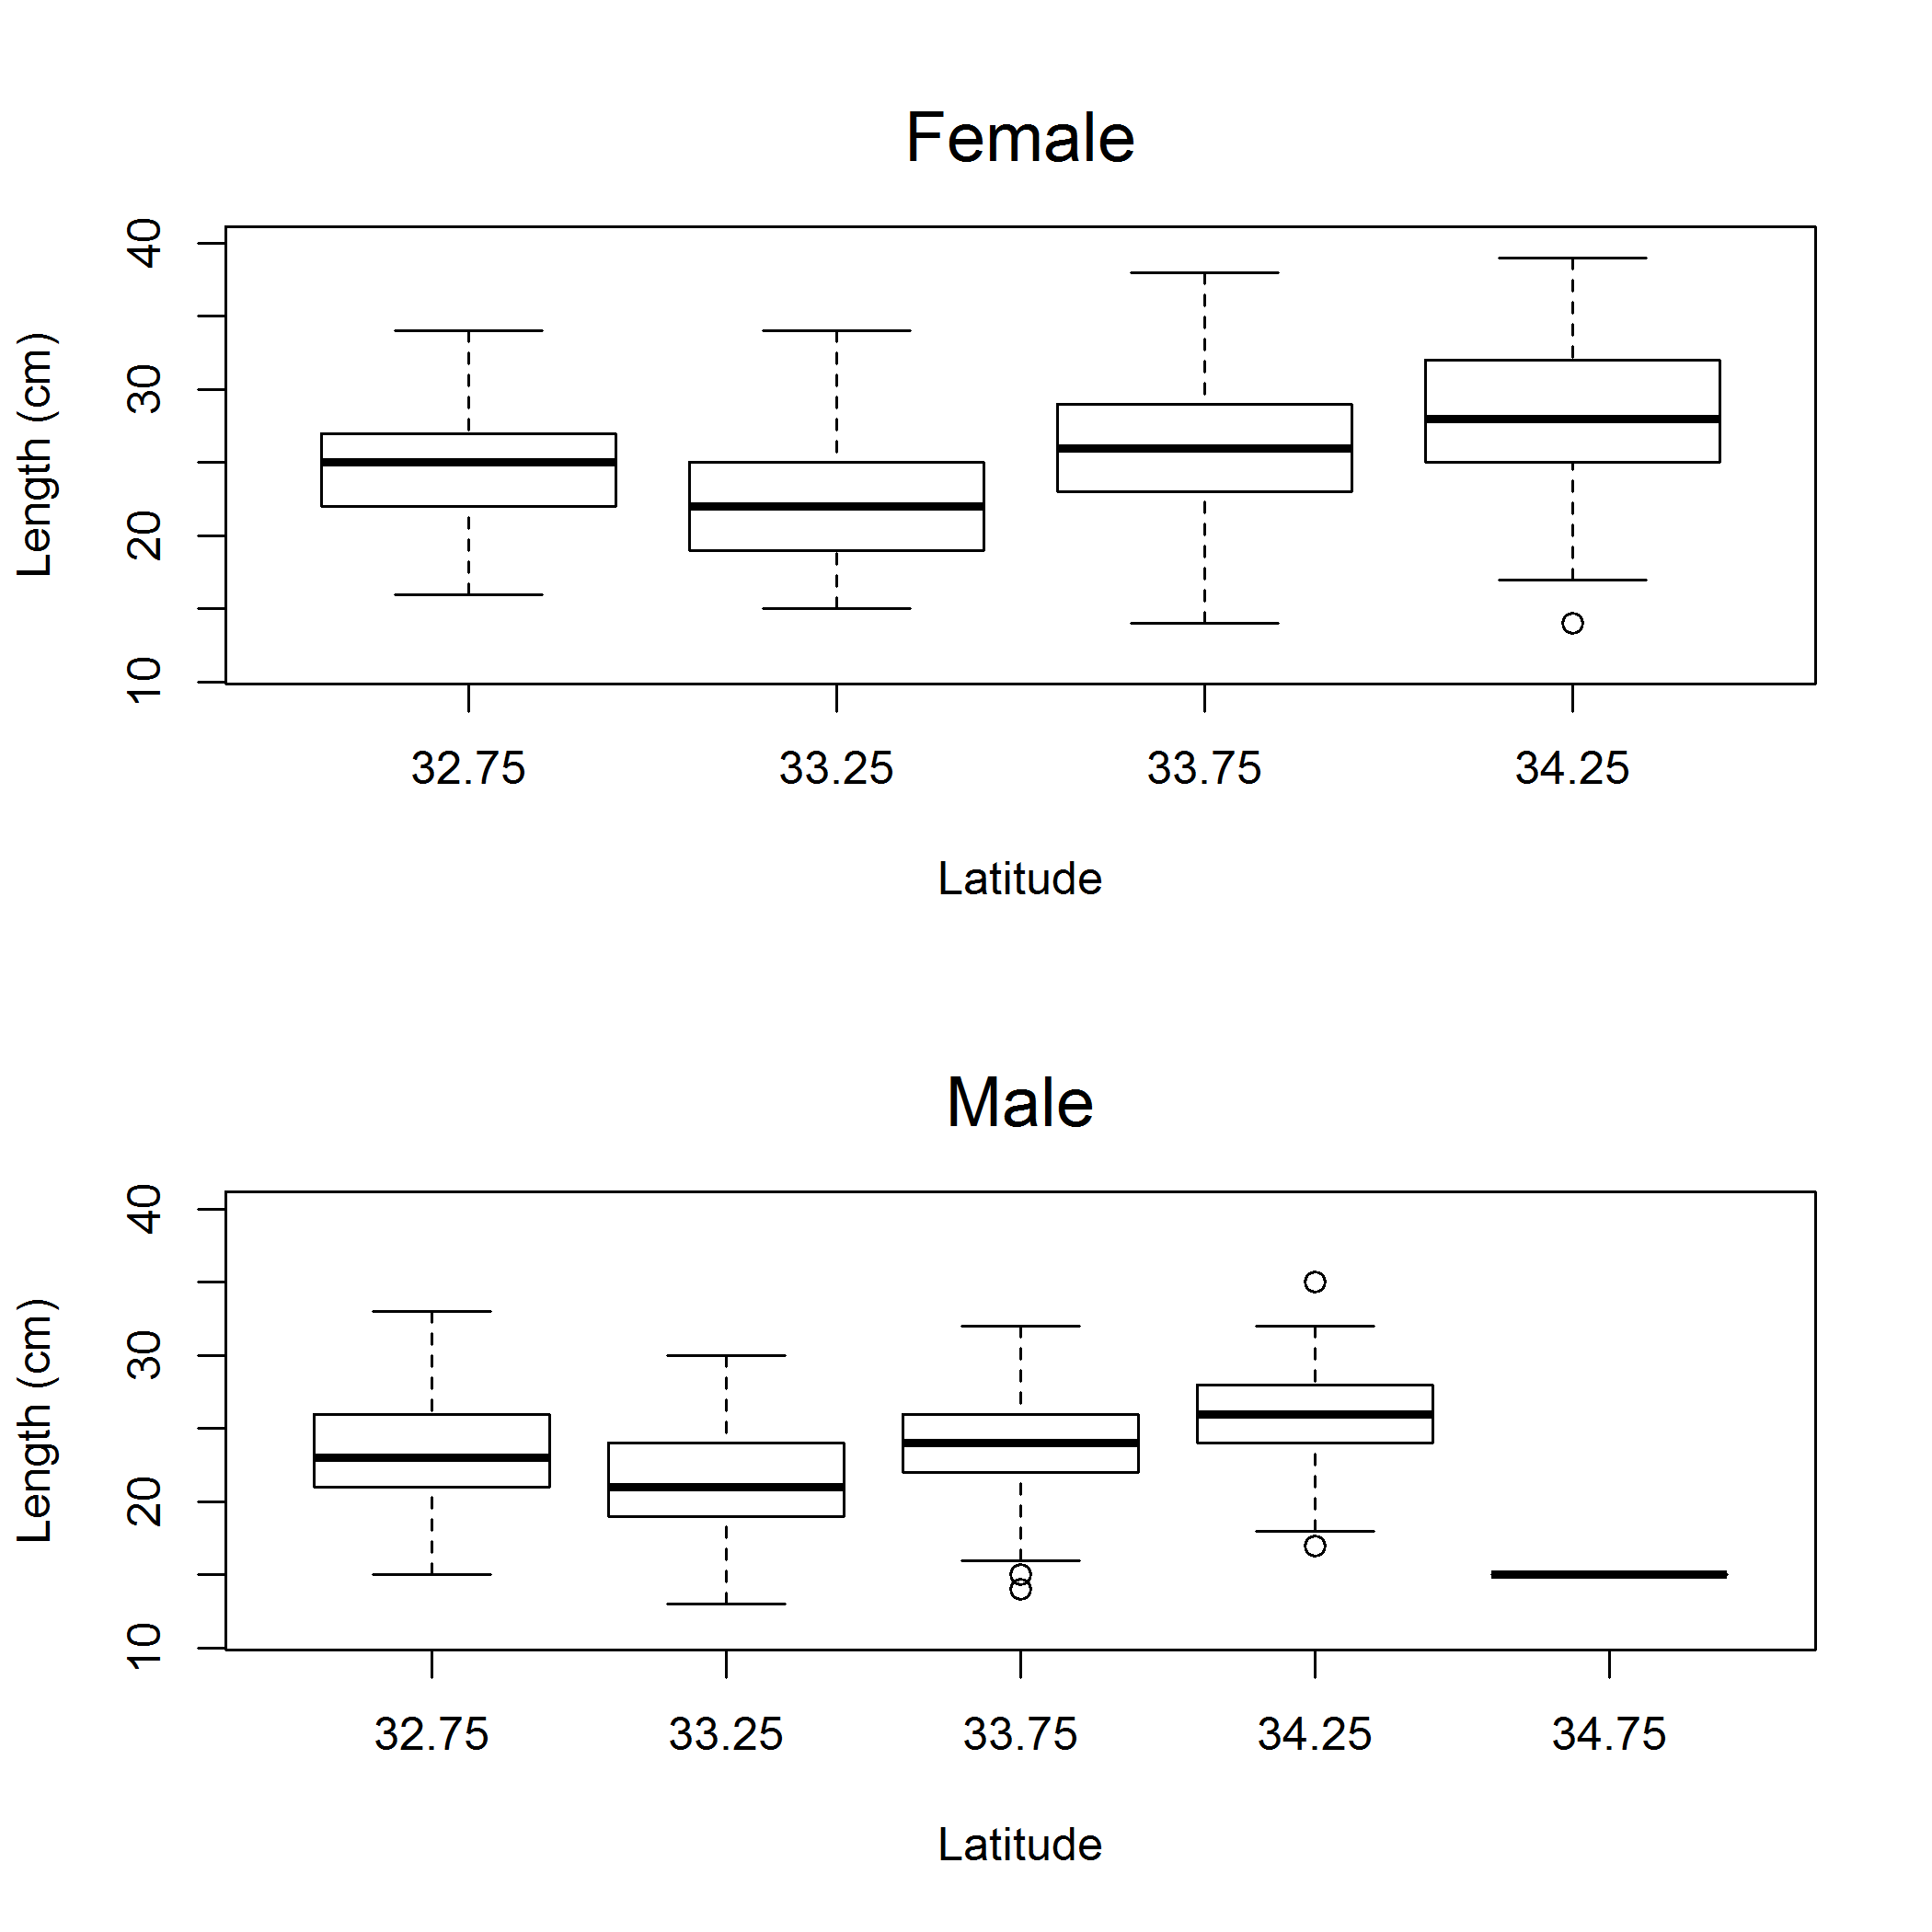
\includegraphics{Figures/NWFSCtrawl_lengthlat.png}
\caption{Comparison box plots of raw length data from NWFSC trawl survey
by latitude zone and sex. \label{fig:Fleet8_NWFSCtrawl_lengthlat}}
\end{figure}

\begin{figure}[htbp]
\centering
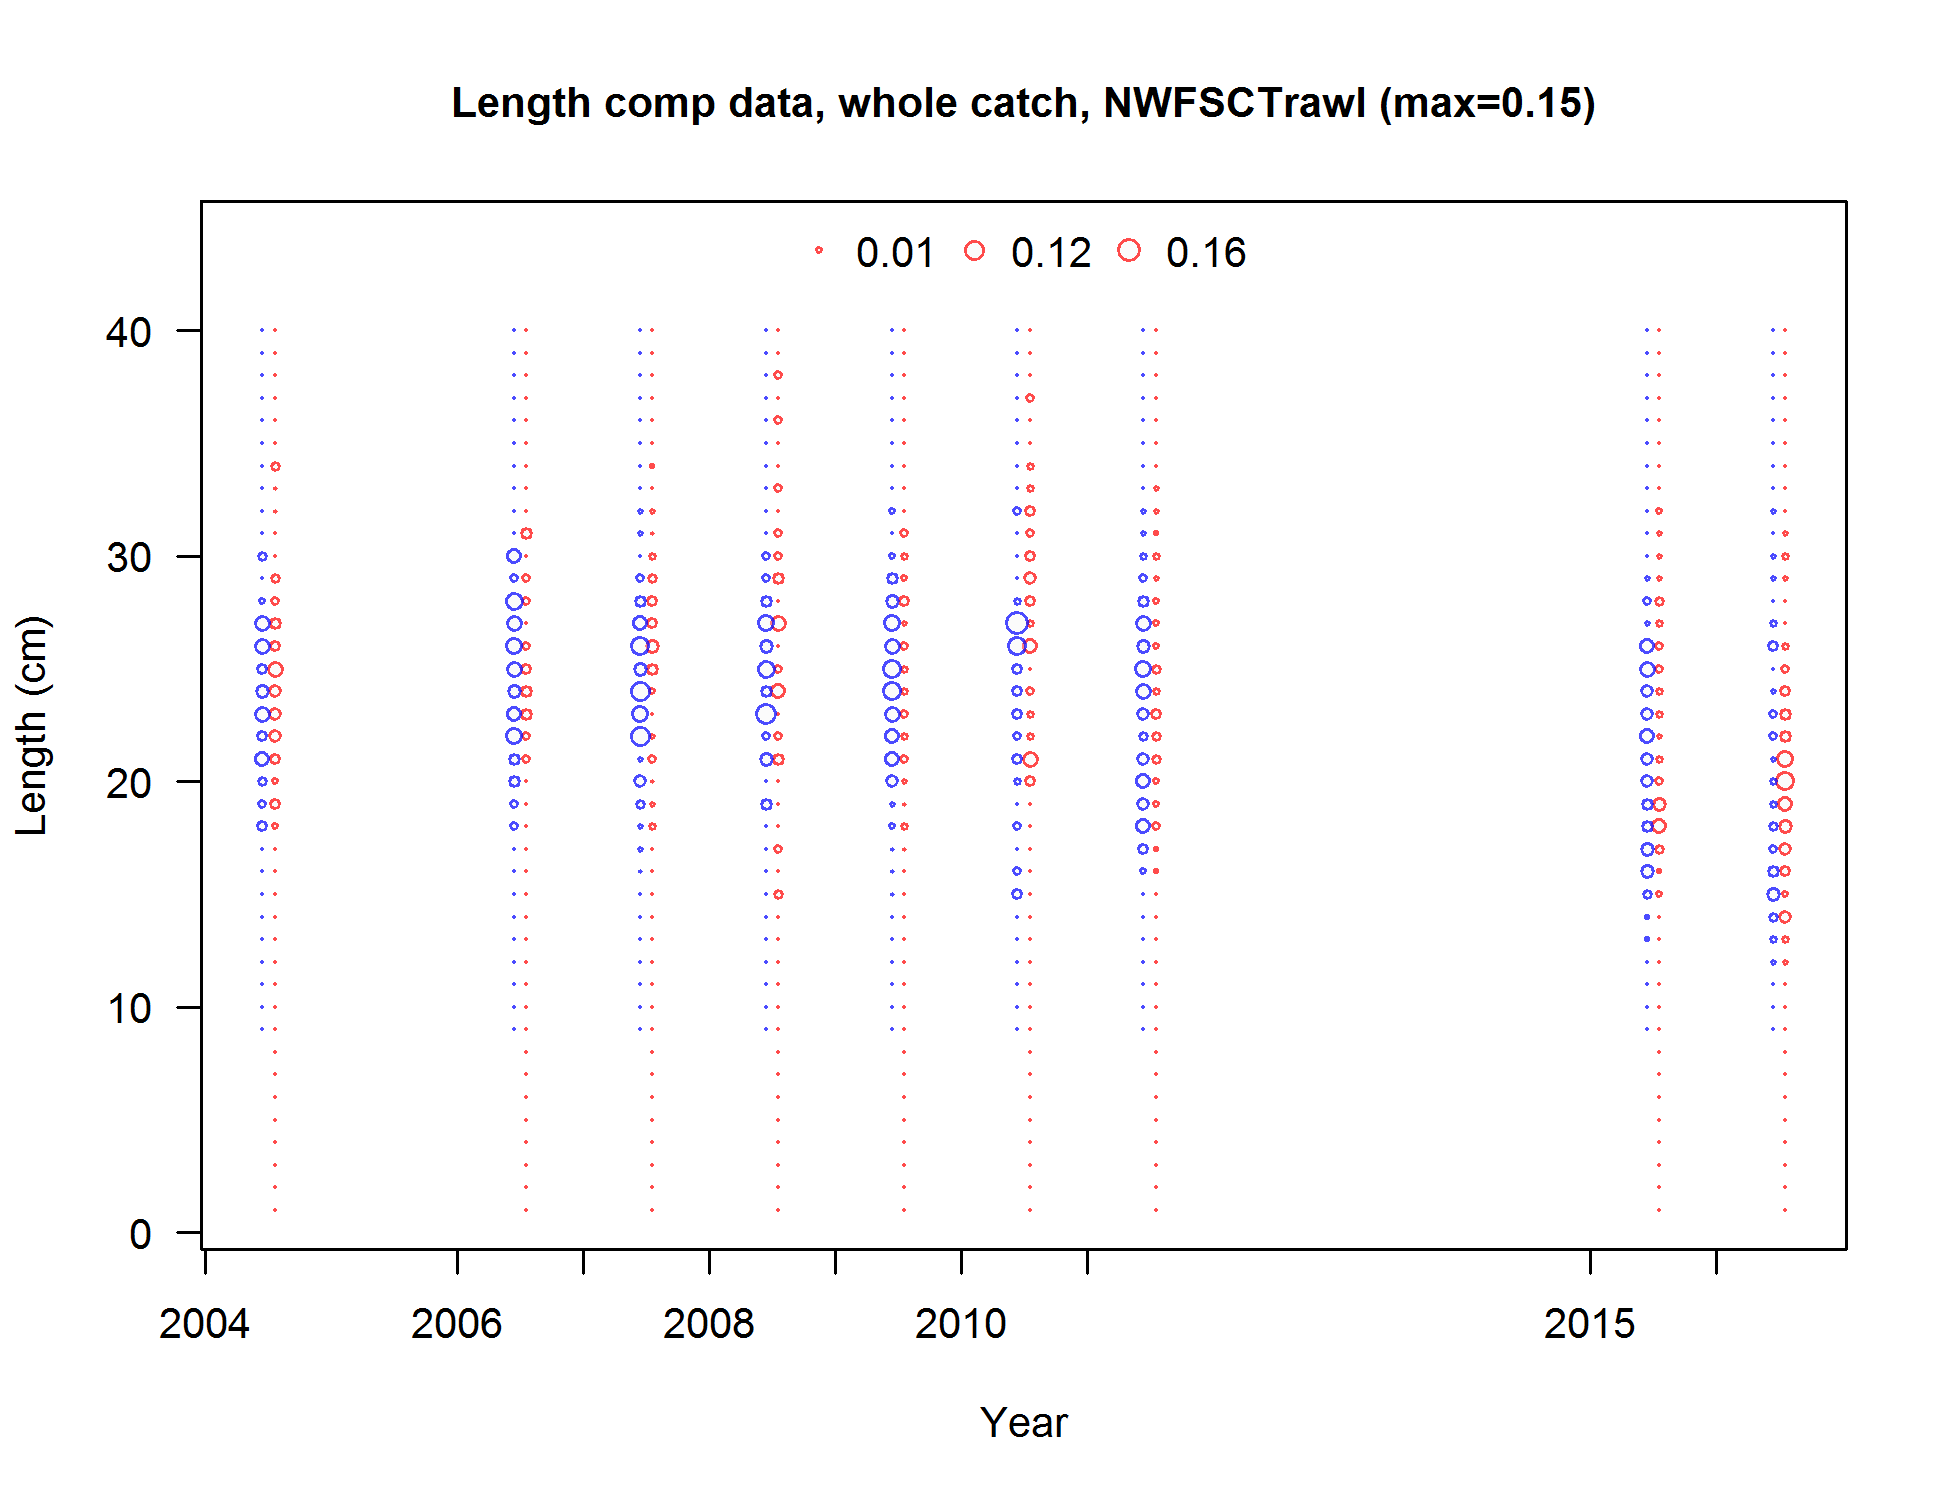
\includegraphics{r4ss/plots_mod1/comp_lendat_bubflt8mkt0.png}
\caption{Length frequency distributions of females (red) and male (blue)
from the NWFSC trawl survey between 2003 and 2016.
\label{fig:Fleet8_comp_lendat_bubflt8mkt0}}
\end{figure}

\begin{figure}[htbp]
\centering
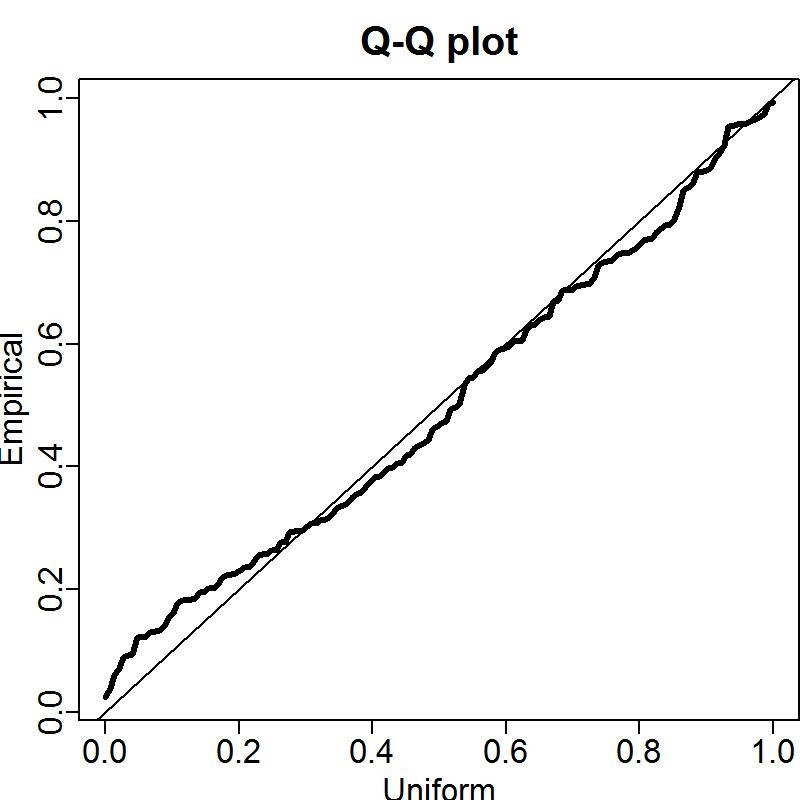
\includegraphics{Figures/NWFSCtrawl_QQ.jpg}
\caption{Q-Q plot used to validate the goodness of fit of the VAST
analysis for the NWFSC trawl survey between 2003 and 2016.
\label{fig:Fleet8_NWFSCtrawl_QQ}}
\end{figure}

\begin{figure}[htbp]
\centering
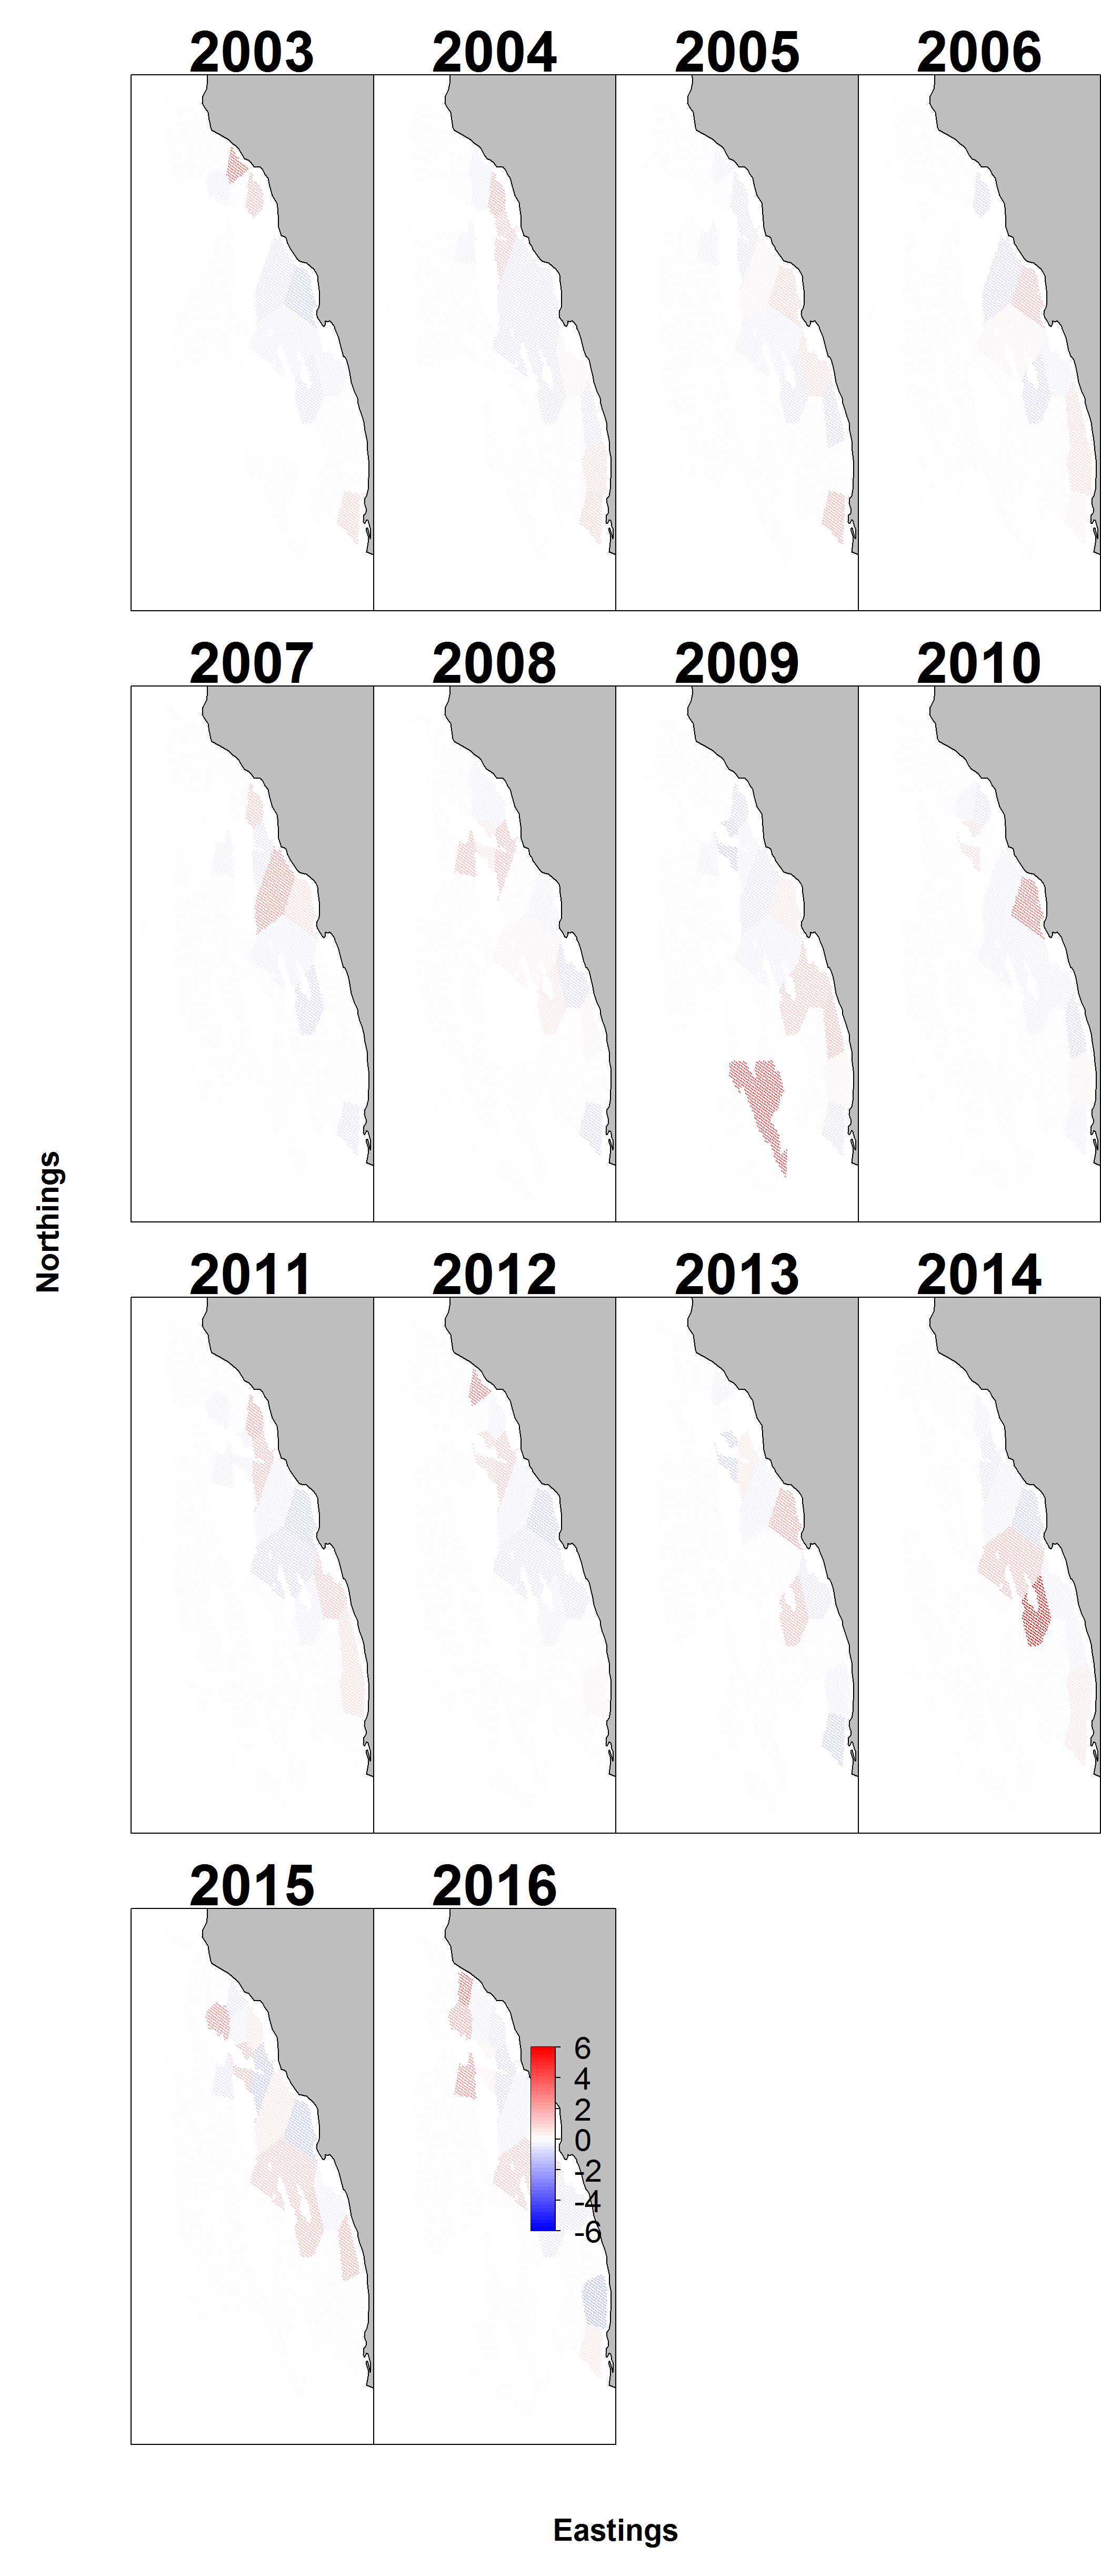
\includegraphics[height=0.95000\textwidth]{Figures/Fleet8_encounter_pearson.png}
\caption{NWFSC survey index encounter probability Pearson residuals
\label{fig:Fleet8_encounter_pearson}}
\end{figure}

\begin{figure}[htbp]
\centering
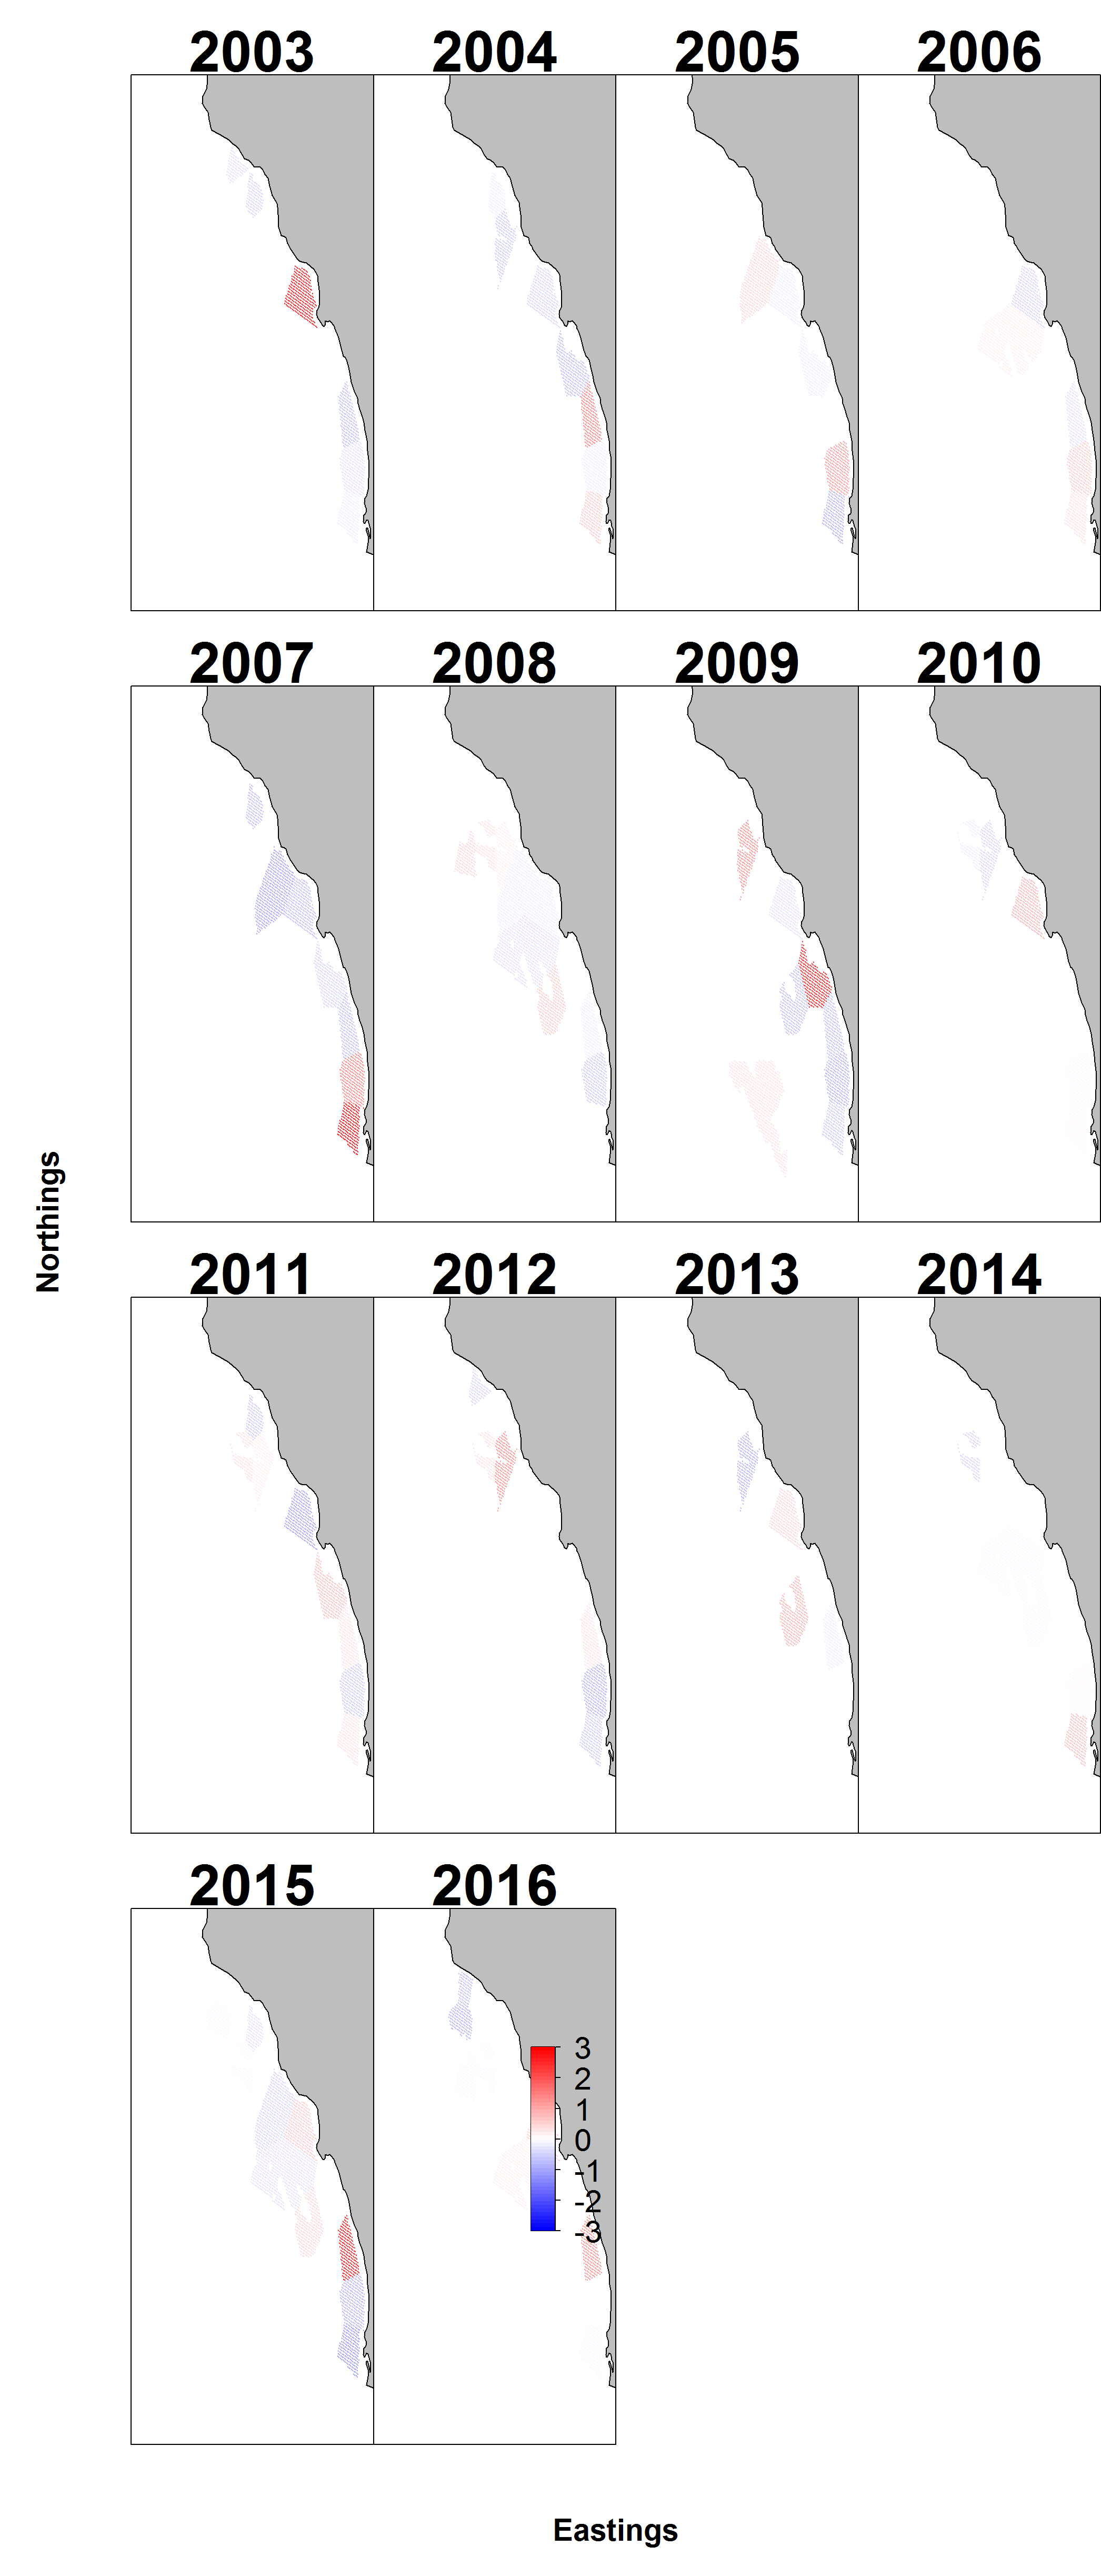
\includegraphics[height=0.95000\textwidth]{Figures/Fleet8_catchrate_pearson.png}
\caption{NWFSC survey index positive catch rate probability Pearson
residuals \label{fig:Fleet8_catchrate_pearson}}
\end{figure}

\begin{figure}[htbp]
\centering
\includegraphics{r4ss/plots_mod1/index4_logcpuedata_NWFSCtrawl.png}
\caption{Standardized index on the log scale for the NWFSC trawl survey
from the VAST analysis from 2003-2016. Lines indicate 95\% uncertainty
interval around index values. Thicker lines indicate input uncertainty
before addition of estimated additional uncertainty parameter.
\label{fig:index4_logcpuedata_NWFSCtrawl}}
\end{figure}

\FloatBarrier

\begin{figure}[htbp]
\centering
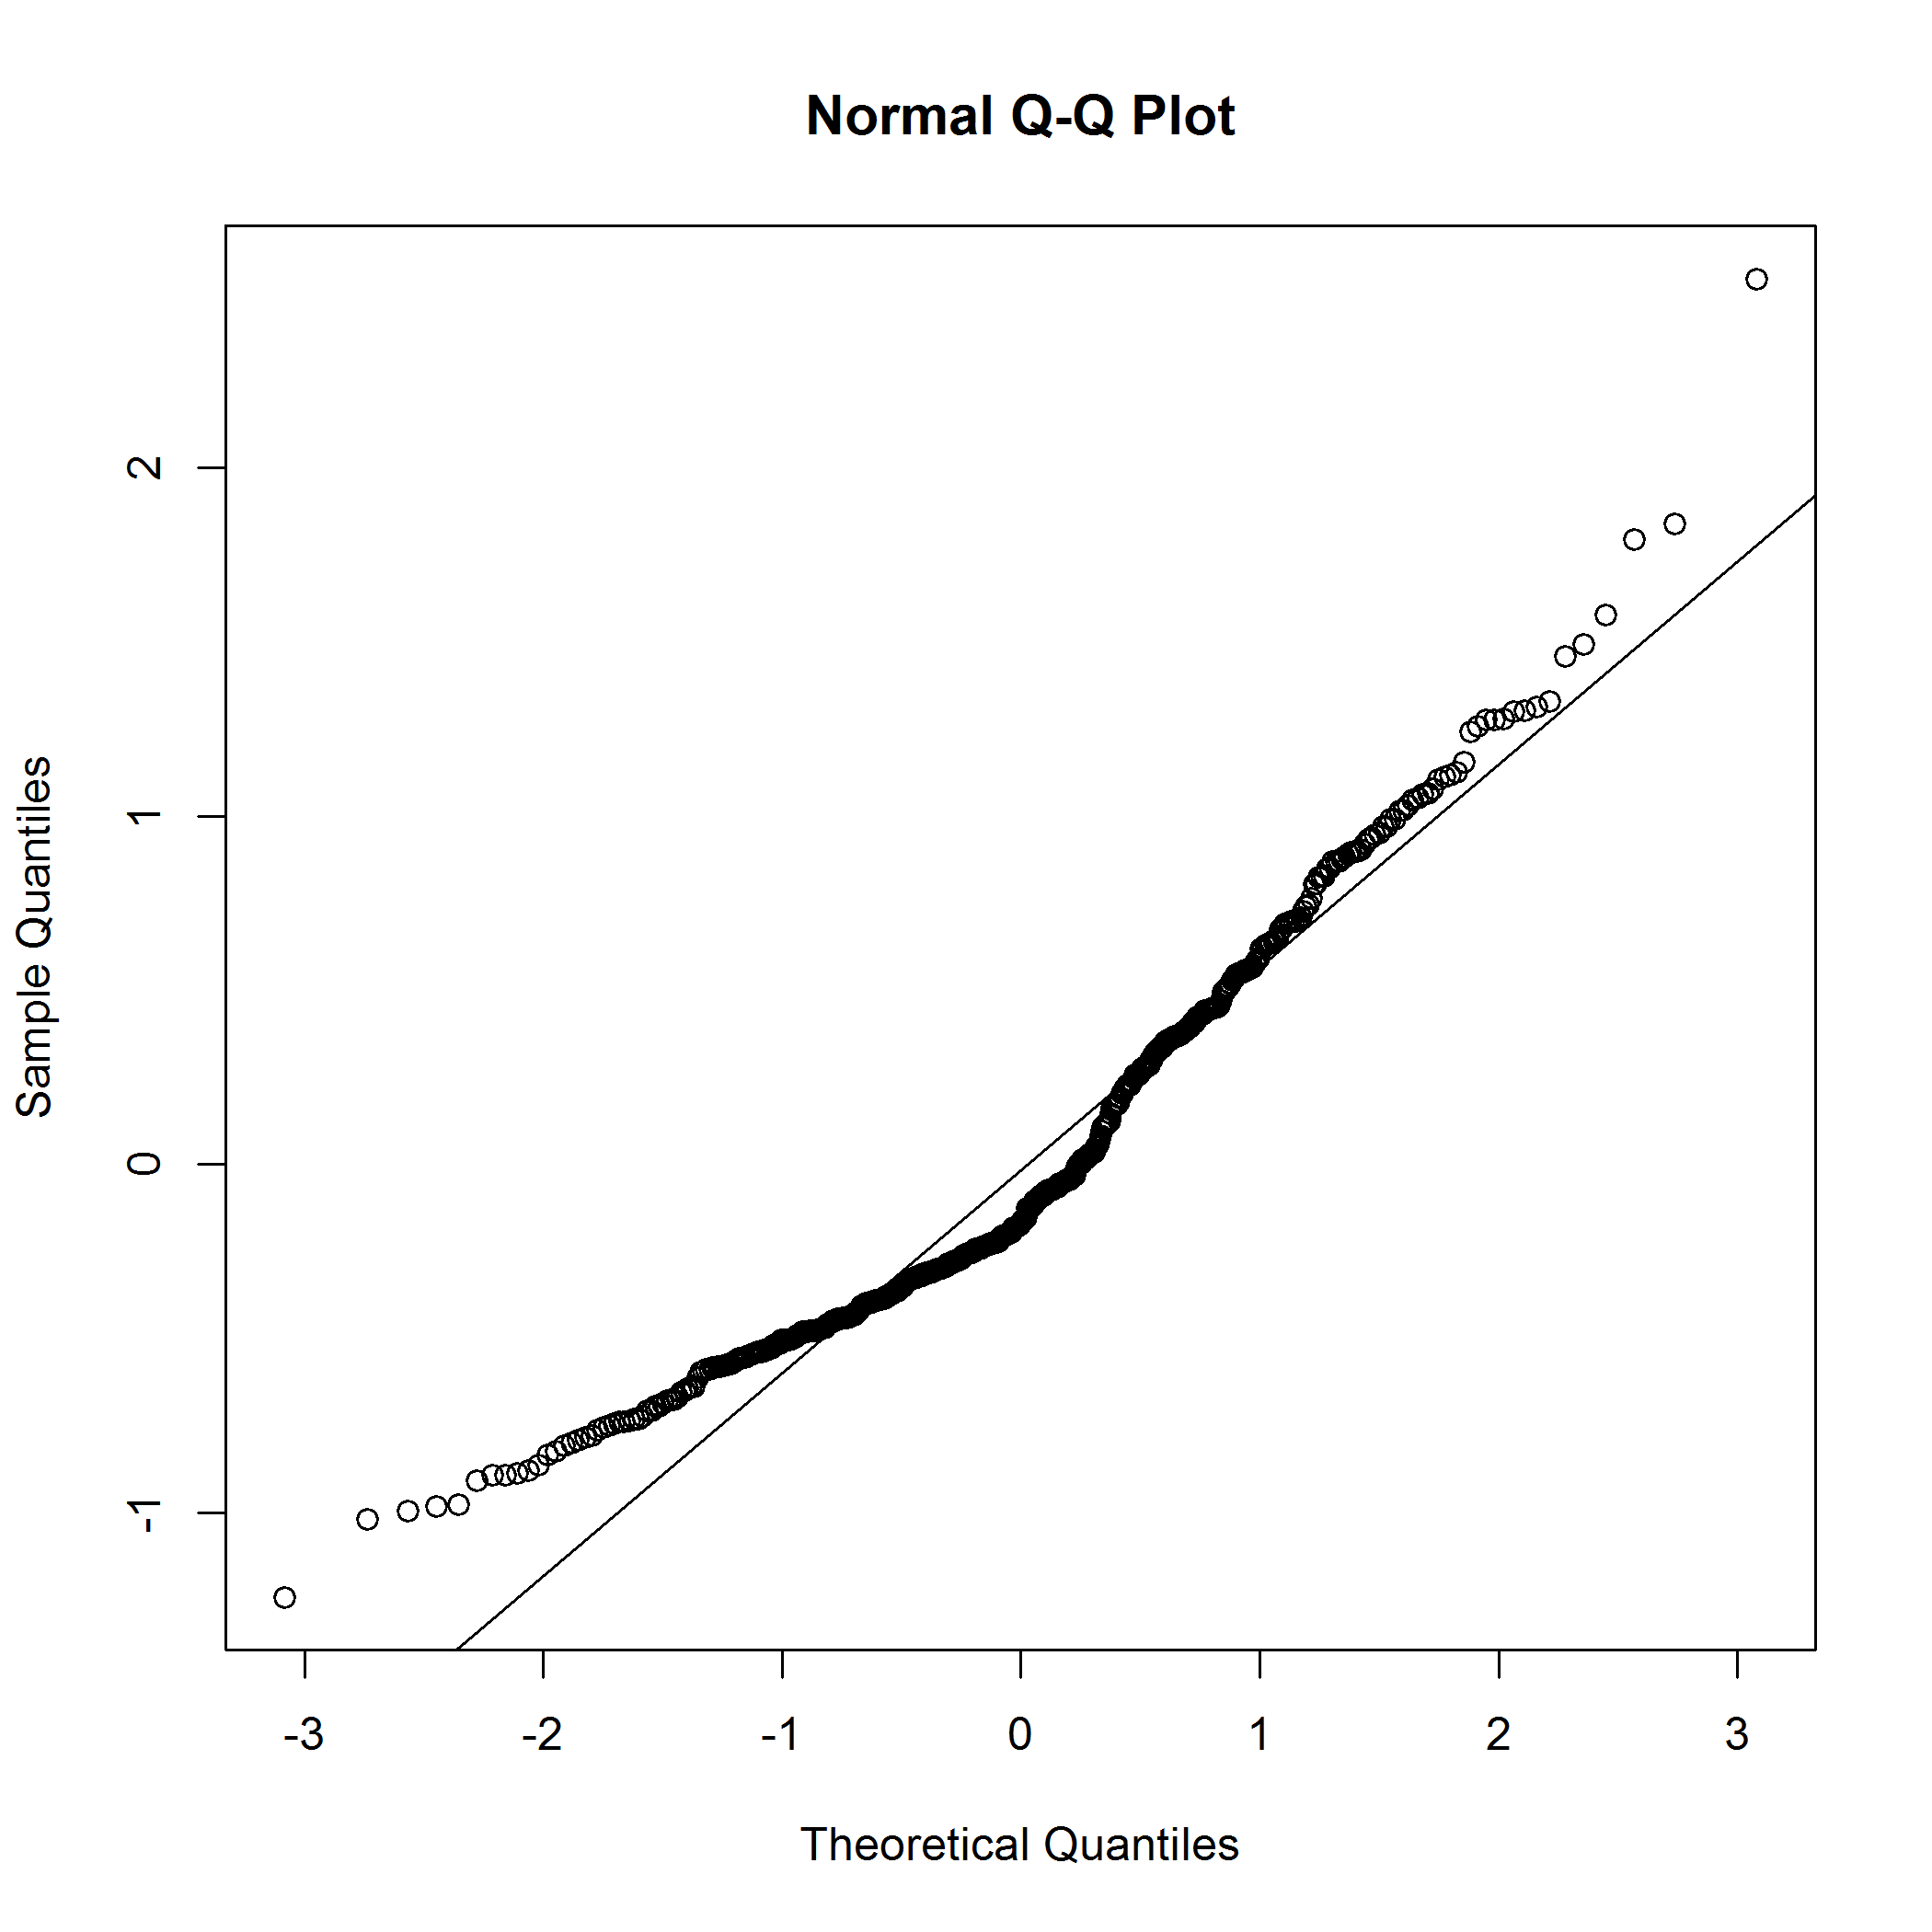
\includegraphics{Figures/Fleet9_GillnetSurvey_QQ.png}
\caption{Q-Q plot used to validate the goodness of fit of the lognormal
model for the CSUN/VRG gillnet survey from 1995-2008.
\label{fig:Fleet9_GillnetSurvey_QQ}}
\end{figure}

\begin{figure}[htbp]
\centering
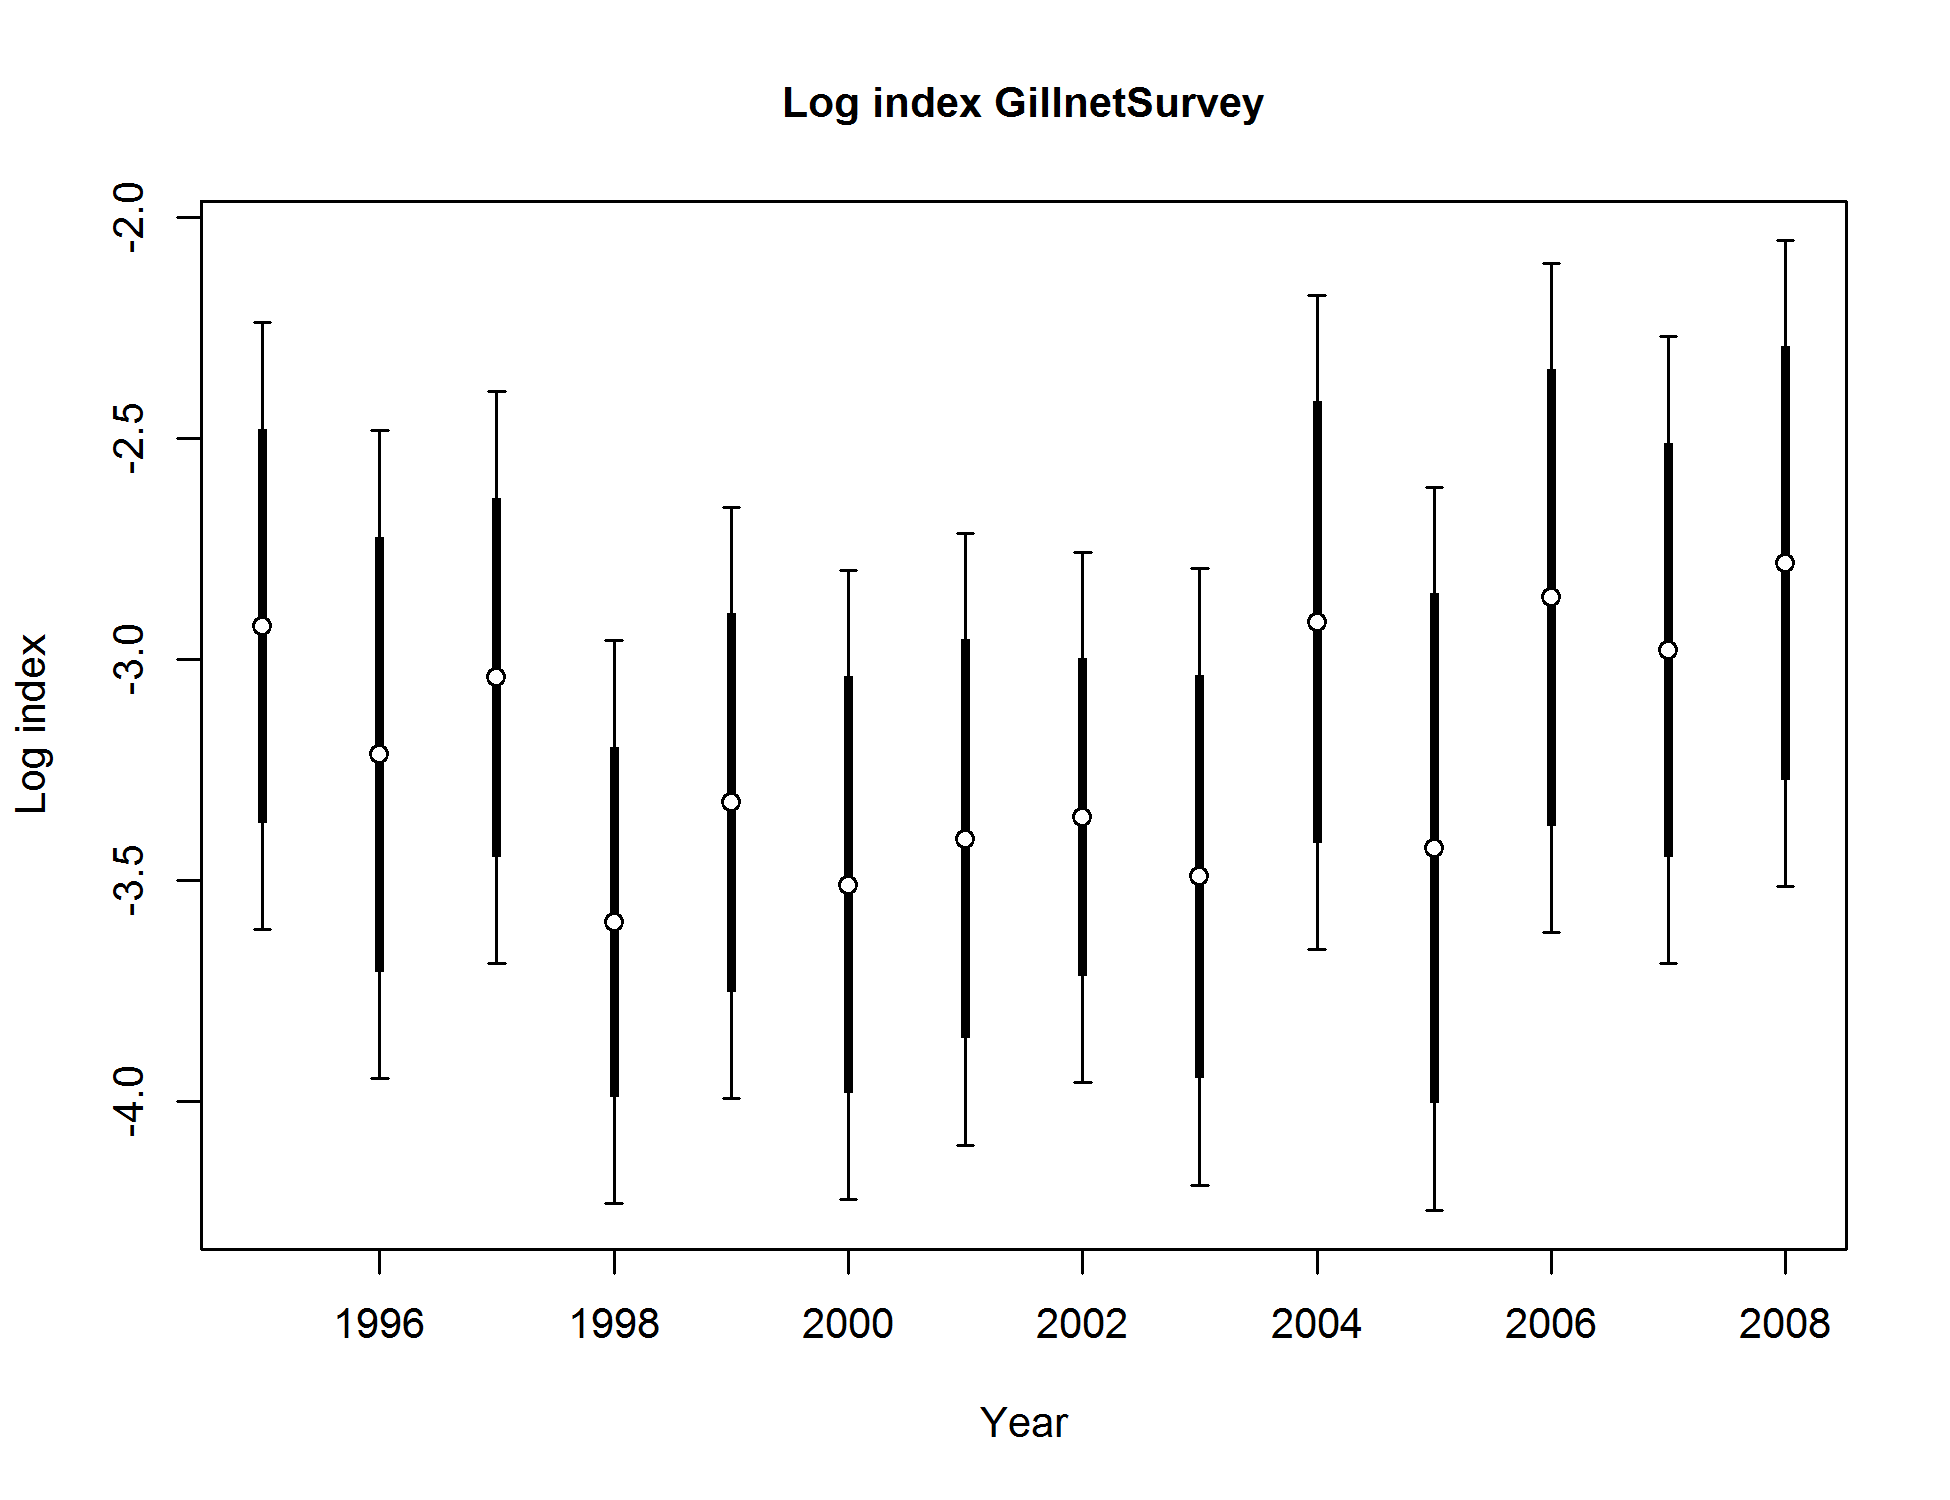
\includegraphics{FIgures/index4_logcpuedata_GillnetSurvey.png}
\caption{Standardized index on the log scale for the recreational
CSUN/VRG gillnet survey. Lines indicate 95\% uncertainty interval around
index values. Thicker lines indicate input uncertainty before addition
of estimated additional uncertainty parameter.
\label{fig:index4_logcpuedata_GillnetSurvey}}
\end{figure}

\begin{figure}[htbp]
\centering
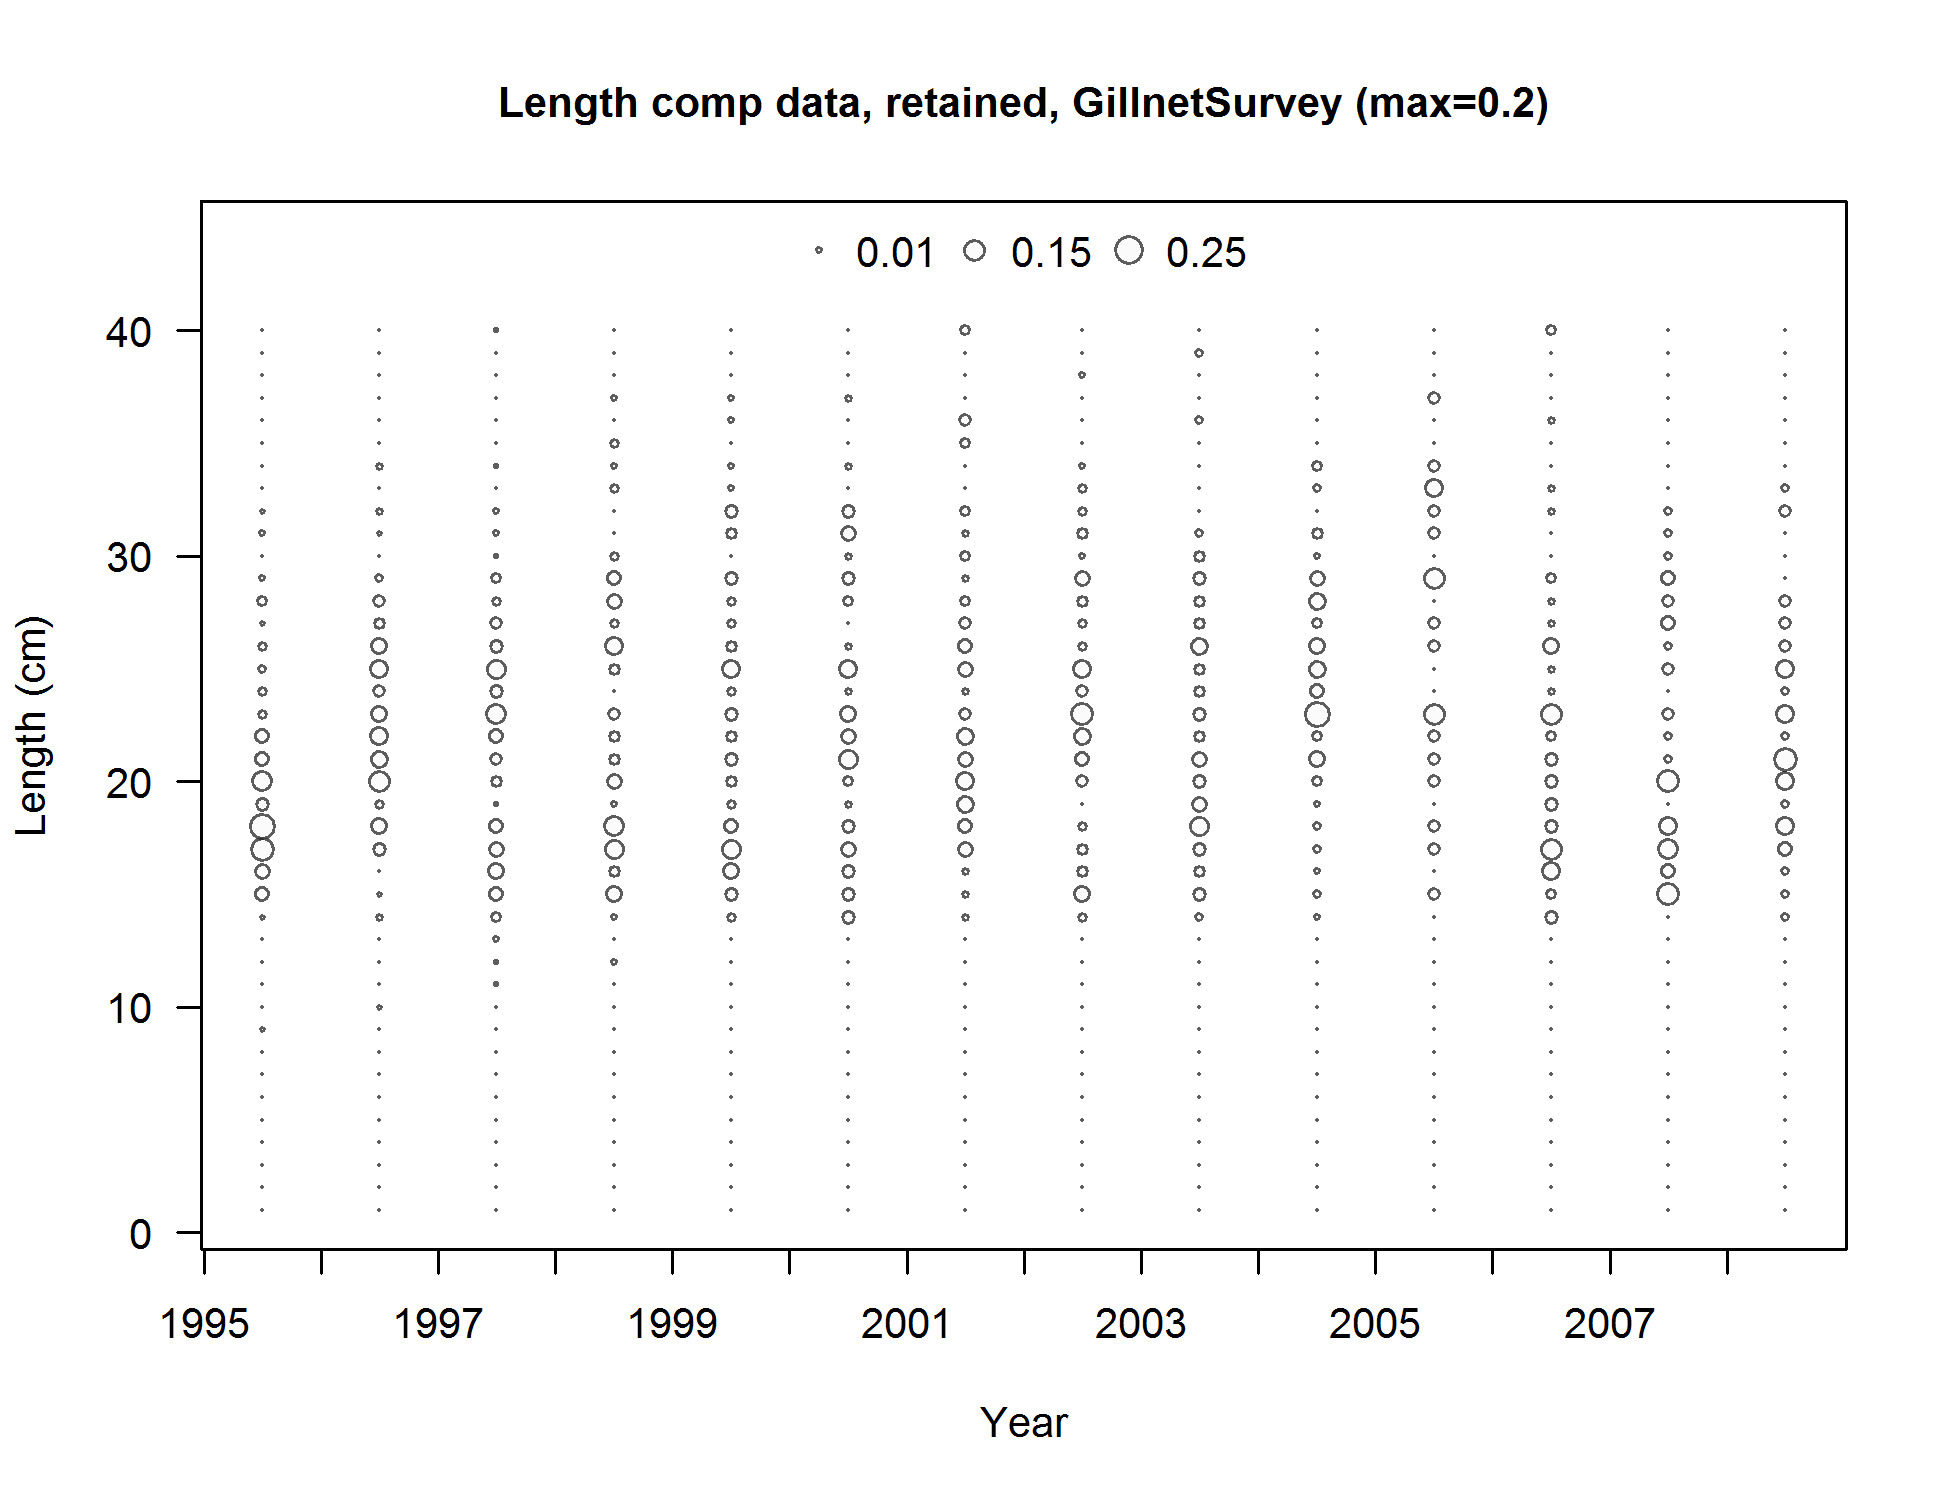
\includegraphics{Figures/comp_lendat_bubflt9mkt2.png}
\caption{Length frequency distributions from the gill net surveys.
\label{fig:Fleet9_GillnetSurvey_lendat_bubflt10mkt2}}
\end{figure}

\FloatBarrier

\begin{figure}[htbp]
\centering
\includegraphics{Figures/Fleet11_SCBSurvey_map.pdf}
\caption{Map of the stations from the Southern California Coastal Water
Research Project regional monitoring trawl survey from 1994, 1998, 2003,
2008, and 2013. Stations used in the index of abundance are colored
magenta. \label{Fleet11_SCBSurvey_map}}
\end{figure}

\begin{figure}[htbp]
\centering
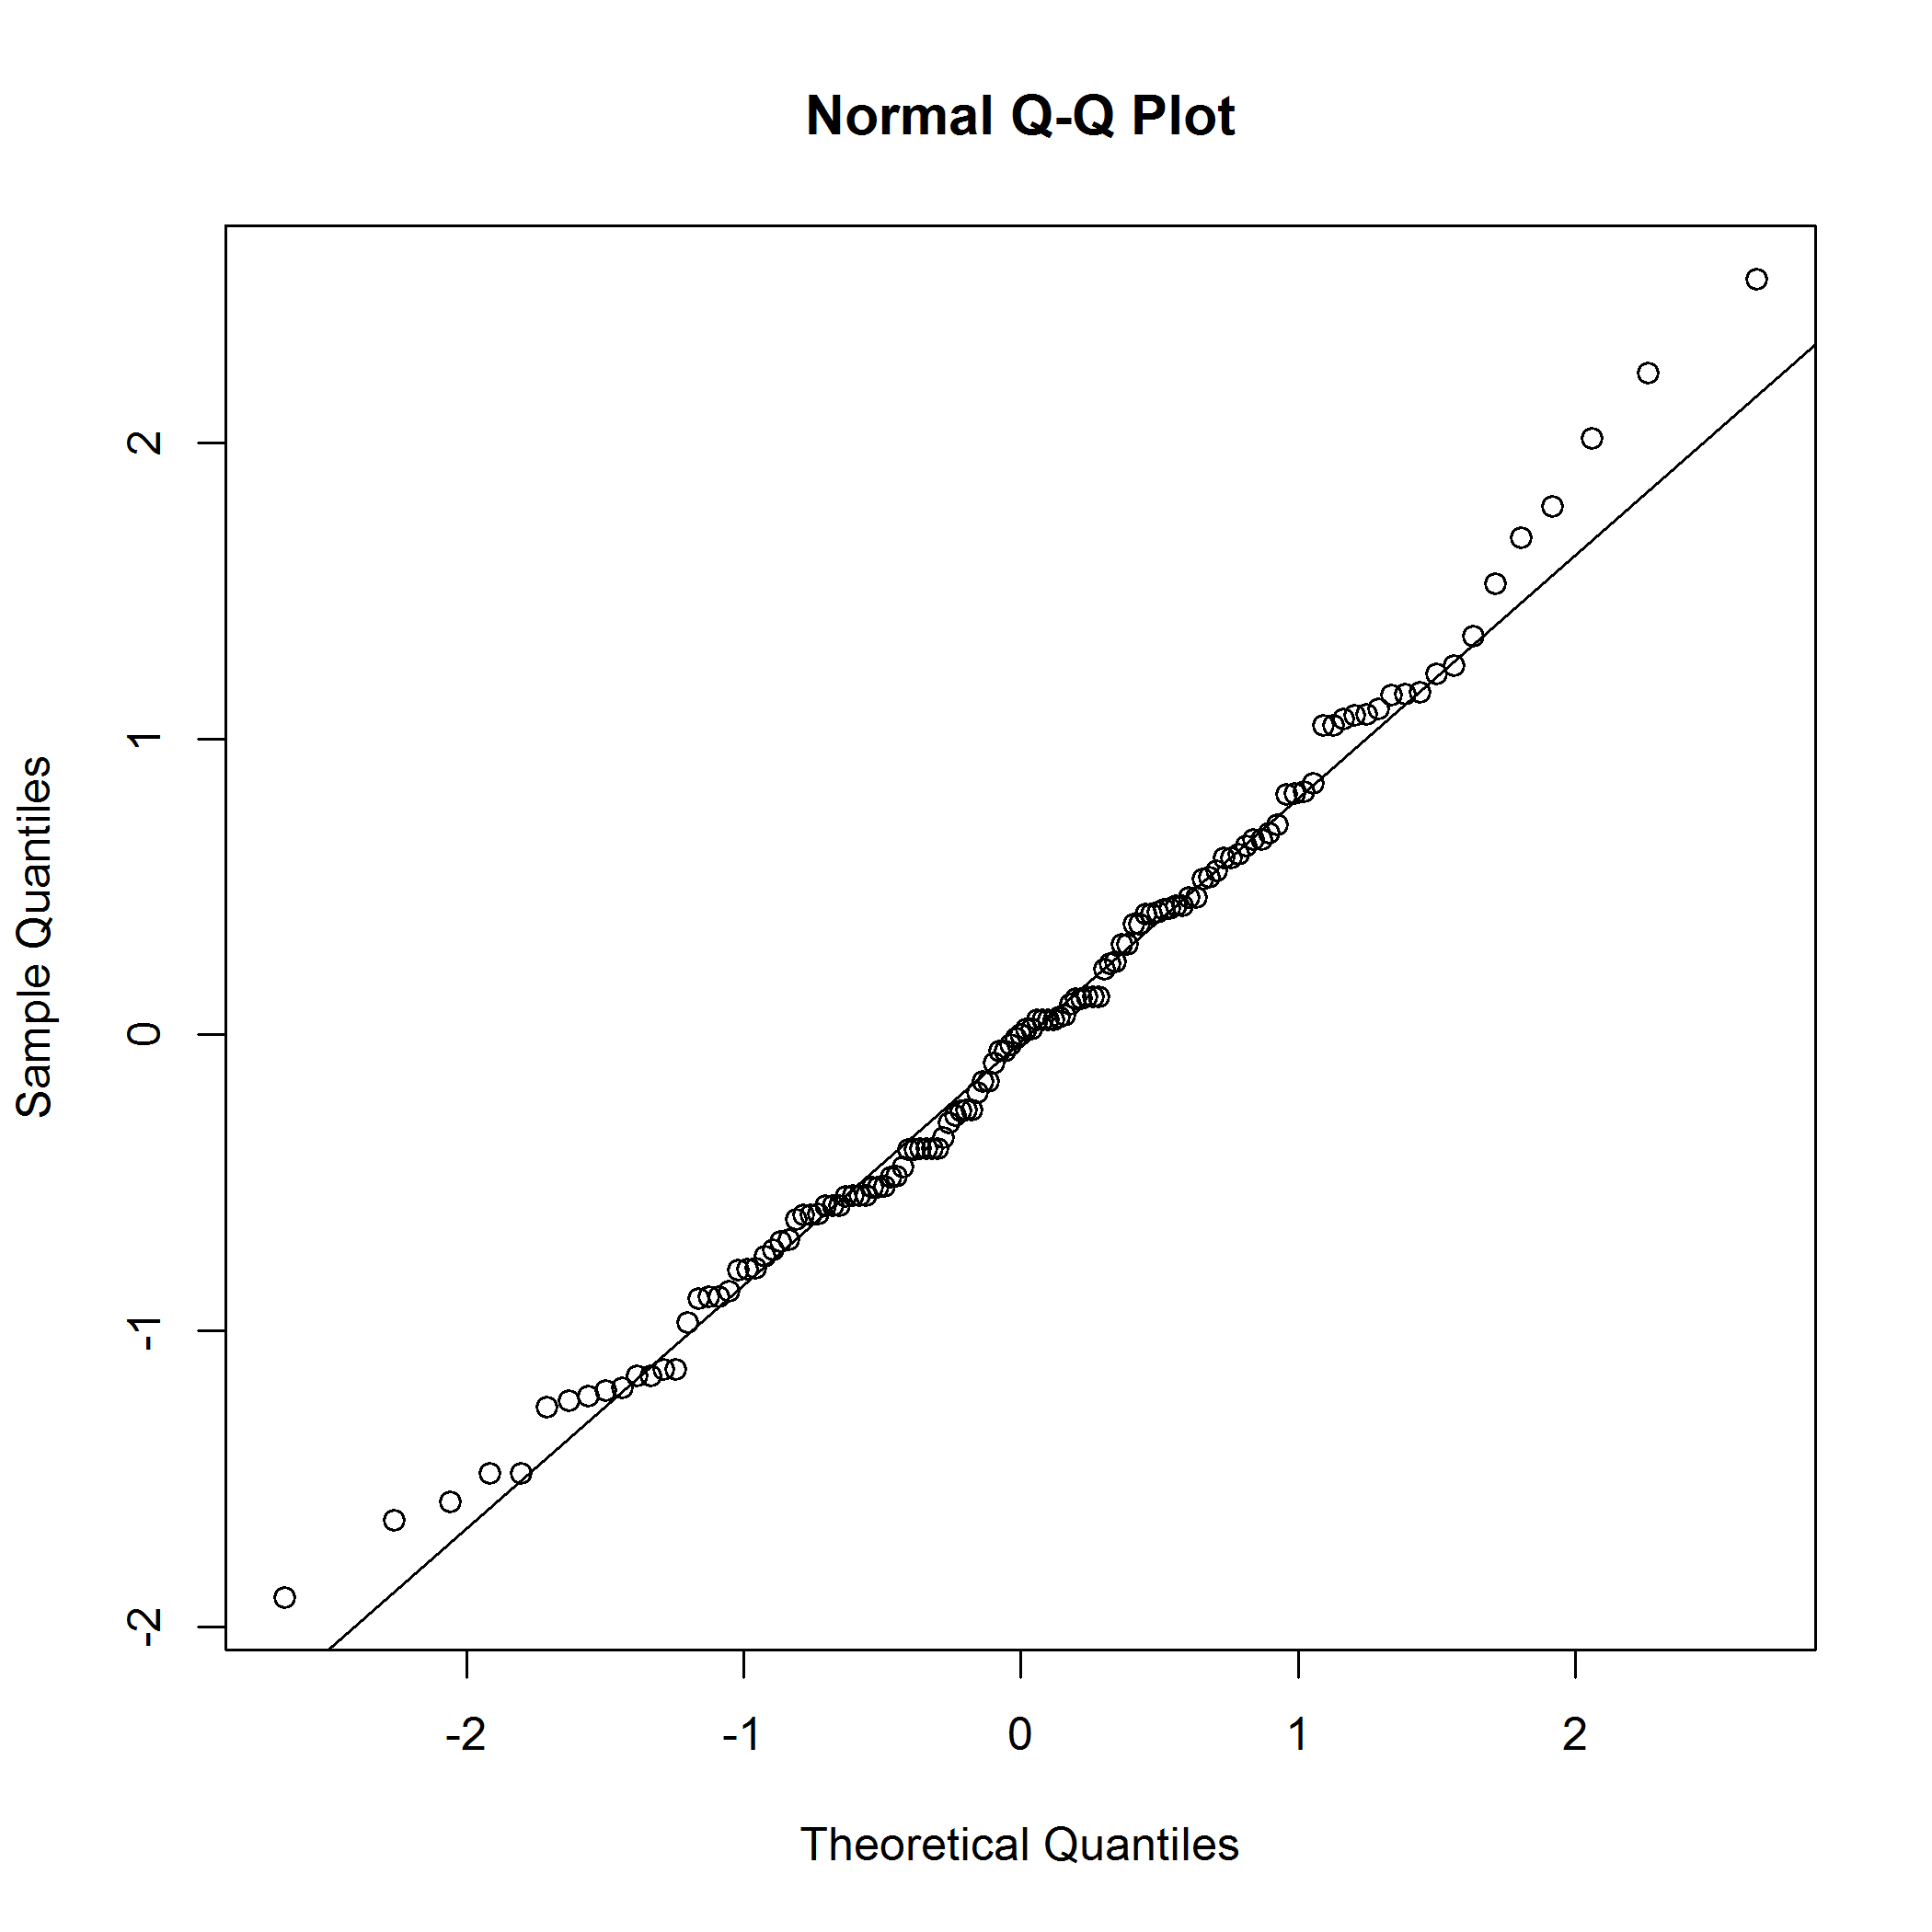
\includegraphics{Figures/Fleet11_SCBsurvey_QQ.png}
\caption{Q-Q plot used to validate the goodness of fit of the lognormal
model for the Southern California Bight monitoring program trawl survey.
\label{fig:Fleet11_SCBsurvey_QQ}}
\end{figure}

\begin{figure}[htbp]
\centering
\includegraphics{r4ss/plots_mod1/index4_logcpuedata_SCBSurvey.png}
\caption{Standardized index on the log scale for the recreational
Southern California Bight trawl survey. Lines indicate 95\% uncertainty
interval around index values. Thicker lines indicate input uncertainty
before addition of estimated additional uncertainty parameter.
\label{fig:index4_logcpuedata_SCBSurvey}}
\end{figure}

\FloatBarrier 

\begin{figure}[htbp]
\centering
\includegraphics{r4ss/plots_mod1/comp_lendat_bubflt11mkt2.png}
\caption{Length frequency distributions from the Southern California
Bight regional monitoring program trawl surveys.
\label{fig:Fleet11_SCBsurvey_lendat_bubflt11mkt2}}
\end{figure}

\begin{figure}[htbp]
\centering
\includegraphics{r4ss/plots_mod1/comp_lendat_bubflt10mkt2.png}
\caption{Length frequency distributions from the Impingement surveys.
\label{fig:Fleet10_comp_lendat_bubflt10mkt2}}
\end{figure}

\FloatBarrier

\begin{figure}[htbp]
\centering
\includegraphics{r4ss/plots_mod1/comp_lendat__aggregated_across_time.png}
\caption{Length comp data, aggregated across time by fleet. Labels
`retained' and `discard' indicate discarded or retained sampled for each
fleet. Panels without this designation represent the whole catch.
\label{fig:comp_lendat_aggregated_across_time}}
\end{figure}

\begin{figure}[htbp]
\centering
\includegraphics{Figures/otolith1.pdf}
\caption{Cross-section of broken and burned California scorpionfish
otolith showing. The green dots indicate the number of increments (photo
courtesy Lance Sullivan, NWFSC). \label{fig:otolith1}}
\end{figure}

\begin{figure}[htbp]
\centering
\includegraphics{Figures/otolith2.pdf}
\caption{California scorpionfish otolith (photo courtesy Lance Sullivan,
NWFSC). \label{fig:otolith2}}
\end{figure}

\FloatBarrier

\begin{figure}[htbp]
\centering
\includegraphics{Figures/Age_length_bySex.png}
\caption{Length at age by sex for California scorpionfish collected from
the NWFSC trawl survey. \label{fig:Agelength}}
\end{figure}

\begin{figure}[htbp]
\centering
\includegraphics{Figures/vonB_compare.png}
\caption{Fitted (external to SS) von Bertalanffy growth by sex for
California scorpionfish collected from the NWFSC trawl survey.
\label{fig:vonB_compare}}
\end{figure}

\begin{figure}[htbp]
\centering
\includegraphics{Figures/Fleet8_NWFSCTrawl_ageerror.png}
\caption{Aging precision between two current age readers at the NWFSC.
Numbers in the bubbles are the sample sizes of otoliths cross-read.
\label{fig:Fleet8_NWFSCTrawl_ageerror}}
\end{figure}

\begin{figure}[htbp]
\centering
\includegraphics{Figures/Fleet8_NWFSCTrawl_ageerror2.pdf}
\caption{True versus predicted age for two current age readers at the
NWFSC from the ageing error software with unbiased reads and curvilinear
standard deviation for both readers.
\label{fig:Fleet8_NWFSCTrawl_ageerror2}}
\end{figure}

\begin{figure}[htbp]
\centering
\includegraphics{Figures/Length_weight.png}
\caption{Comparison of the California scorpionfish weight-length curves
from Love et al. (1987) and those estimated from the NWFSC trawl survey.
The latter is used in this assessment. \label{fig:Length_weight}}
\end{figure}

\FloatBarrier

\begin{figure}[htbp]
\centering
\includegraphics{Figures/bridge_harvestrate.png}
\caption{Time series of harvest rates by fleet from the 2005 model where
the harvest rate for the recreational fleet hit the boundary of 0.9.
\label{fig:bridge_harvestrate}}
\end{figure}

\begin{figure}[htbp]
\centering
\includegraphics{Figures/bridge_catch.png}
\caption{Time series of observed and expected landings by fleet from the
2005 model. The model was not able to remove all of the recreational
catches starting around 1970. \label{fig:bridge_catch}}
\end{figure}

\begin{figure}[htbp]
\centering
\includegraphics[height=0.95000\textwidth]{Figures/bridge_timeseries.png}
\caption{Comparison of spawning output, total biomass, and recruits from
the 2005 model (solid red lines) using SS2, the 2005 model converted to
SS3.24z (blue lines), and the pre-STAR base model from this assessment
(purple lines). Note: The 2005 assessment was found to have an error,
and therefore the time series for the model to SS3.24 will not match
perfectly. \label{fig:bridge_timeseries}}
\end{figure}

\begin{figure}[htbp]
\centering
\includegraphics{Figures/Request1.png}
\caption{Selectivity curves for the dead discard fleet with three (left)
or two (right) time blocks. \label{fig:Request1}}
\end{figure}

\vspace{5cm}

\begin{figure}[htbp]
\centering
\includegraphics{Figures/Request3a.png}
\caption{Comparison of the recreational private mode dockside index
using three different thresholds for the Stephens-MacCall filter.
\label{fig:Request3a}}
\end{figure}

\begin{figure}[htbp]
\centering
\includegraphics{Figures/Request3b.png}
\caption{Comparisons of the base model using the index developed for the
recreational private mode dockside index using three different
thresholds for the Stephens-MacCall filter.\label{fig:Request3b}}
\end{figure}

\newpage

\begin{figure}[htbp]
\centering
\includegraphics{Figures/Request8.png}
\caption{Time series of estimated recruitment deviations from the base
model and the CalCOFI sea surface temperature. \label{fig:Request8}}
\end{figure}

\begin{figure}[htbp]
\centering
\includegraphics[height=0.90000\textwidth]{Figures/Request9.png}
\caption{Time series of relative spawning biomass (top) and spawning
biomass (bottom) from the base model compared to a model with no
recruitment deviations and a sigma-r of 0.3. \label{fig:Request9}}
\end{figure}

\begin{figure}[htbp]
\centering
\includegraphics[height=0.90000\textwidth]{Figures/Request12.png}
\caption{Time series of spawning biomass (top) and relative spawning
biomass (bottom) from the pre-STAR base model (M fixed at 0.257 for
females and estimated for males) compared to the STAR panel base model
(one M = 0.235), and the two states of nature of natural mortality of
0.165 and 0.2745. \label{fig:Request12}}
\end{figure}

\FloatBarrier

\FloatBarrier

\FloatBarrier

\begin{figure}[htbp]
\centering
\includegraphics{r4ss/plots_mod1/sel01_multiple_fleets_length1.png}
\caption{Selectivity at length for all of the fleets in the base model.
\label{fig:sel01_multiple_fleets_length1}}
\end{figure}

\begin{figure}[htbp]
\centering
\includegraphics{r4ss/plots_mod1/sel03_len_timevary_surf_flt1sex1.png}
\caption{Surface plot of Female time-varying selectivity for the
commercial hook-and-line fleet, with time blocks from 1916-1998 and
1999-2016. \label{fig:sel03_len_timevary_surf_flt1sex1}}
\end{figure}

\begin{figure}[htbp]
\centering
\includegraphics{r4ss/plots_mod1/sel03_len_timevary_surf_flt4sex1.png}
\caption{Surface plot of Female time-varying selectivity for the
recreational private boat fleet, with time blocks from 1916-2000,
2001-2005, and 2006-2016. \label{fig:sel03_len_timevary_surf_flt4sex1}}
\end{figure}

\begin{figure}[htbp]
\centering
\includegraphics{r4ss/plots_mod1/sel03_len_timevary_surf_flt5sex1.png}
\caption{Surface plot of Female time-varying selectivity for the
recreational party/charter retained-only catch fleet, with time blocks
from 1916-2000, 2001-2005, and 2006-2016.
\label{fig:sel03_len_timevary_surf_flt5sex1}}
\end{figure}

\FloatBarrier

\begin{figure}[htbp]
\centering
\includegraphics{r4ss/plots_mod1/recdevs2_withbars.png}
\caption{Estimated time-series of recruitment deviations for California
scorpionfish with 95\% intervals. \label{fig:recdevs2_withbars}}
\end{figure}

\begin{figure}[htbp]
\centering
\includegraphics{r4ss/plots_mod1/ts11_Age-0_recruits_(1000s)_with_95_asymptotic_intervals.png}
\caption{Estimated time-series of recruitment for California
scorpionfish.
\label{fig:ts11_Age-0_recruits_(1000s)_with_95_asymptotic_intervals}}
\end{figure}

\begin{figure}[htbp]
\centering
\includegraphics{r4ss/plots_mod1/SR_curve2.png}
\caption{Estimated recruitment (red circles) and the assumed
stock-recruit relationship (black line) for California scorpionfish. The
green line shows the effect of the bias correction for the lognormal
distribution. \label{fig:SR_curve2}}
\end{figure}

\begin{figure}[htbp]
\centering
\includegraphics{r4ss/plots_mod1/index5_logcpuefit_RecPR.png}
\caption{Fit to log index data on log scale for the CRFS recreational
private mode fishery. Lines indicate 95\% uncertainty interval around
index values. Thicker lines indicate input uncertainty before addition
of estimated additional uncertainty parameter.
\label{fig:index5_logcpuefit_RecPR}}
\end{figure}

\begin{figure}[htbp]
\centering
\includegraphics{r4ss/plots_mod1/index5_logcpuefit_RecPC.png}
\caption{Fit to log index data on log scale for the recreational CPFV
logbook retained catches. Lines indicate 95\% uncertainty interval
around index values. Thicker lines indicate input uncertainty before
addition of estimated additional uncertainty parameter.
\label{fig:index5_logcpuefit_RecPC}}
\end{figure}

\begin{figure}[htbp]
\centering
\includegraphics{r4ss/plots_mod1/index5_logcpuefit_RecDD.png}
\caption{Fit to log index data on log scale for the recreational CPFV
onboard observer discard catch index. Lines indicate 95\% uncertainty
interval around index values. Thicker lines indicate input uncertainty
before addition of estimated additional uncertainty parameter.
\label{fig:Fleet6_index5_logcpuefit_RecDD}}
\end{figure}

\begin{figure}[htbp]
\centering
\includegraphics{r4ss/plots_mod1/index5_logcpuefit_RecPCOBR.png}
\caption{Fit to log index data on log scale for the recreational CPFV
onboard observer retained catch index. Lines indicate 95\% uncertainty
interval around index values. Thicker lines indicate input uncertainty
before addition of estimated additional uncertainty parameter.
\label{fig:Fleet12_index5_logcpuefit_RecPCOBR}}
\end{figure}

\begin{figure}[htbp]
\centering
\includegraphics{r4ss/plots_mod1/index5_logcpuefit_Sanitation.png}
\caption{Fit to log index data on log scale for the POTW trawl index.
Lines indicate 95\% uncertainty interval around index values. Thicker
lines indicate input uncertainty before addition of estimated additional
uncertainty parameter. \label{fig:index5_logcpuefit_Sanitation}}
\end{figure}

\begin{figure}[htbp]
\centering
\includegraphics{r4ss/plots_mod1/index5_logcpuefit_NWFSCtrawl.png}
\caption{Fit to log index data on log scale for the NWFSC trawl survey
from the VAST analysis from 2003-2016. Lines indicate 95\% uncertainty
interval around index values. Thicker lines indicate input uncertainty
before addition of estimated additional uncertainty parameter.
\label{fig:index5_logcpuefit_NWFSCtrawl}}
\end{figure}

\begin{figure}[htbp]
\centering
\includegraphics{r4ss/plots_mod1/index5_logcpuefit_SCBSurvey.png}
\caption{Fit to log index data on log scale for the recreational
Southern California Bight trawl survey. Lines indicate 95\% uncertainty
interval around index values. Thicker lines indicate input uncertainty
before addition of estimated additional uncertainty parameter.
\label{fig:index5_logcpuefit_SCBSurvey}}
\end{figure}

\begin{figure}[htbp]
\centering
\includegraphics{r4ss/plots_mod1/comp_lenfit__aggregated_across_time.png}
\caption{Length compositions aggregated across time by fleet. Labels
`retained' and `discard' indicate retained or discarded samples for each
fleet. Panels without this designation represent the whole catch.
\label{fig:comp_lenfit__aggregated_across_time}}
\end{figure}

\FloatBarrier

\begin{figure}[htbp]
\centering
\includegraphics{./r4ss/plots_mod1/comp_condAALfit_Andre_plotsflt8mkt0_page1.png}
\caption{Conditional AAL plot, whole catch, NWFSCTrawl (plot 1 of 4)
These plots show mean age and std. dev. in conditional AAL. Left plots
are mean AAL by size\_class (obs. and pred.) with 90\% CIs based on
adding 1.64 SE of mean to the data. Right plots in each pair are SE of
mean AAL (obs. and pred.) with 90\% CIs based on the chi\_square
distribution.
\label{fig:mod1_4_comp_condAALfit_Andre_plotsflt8mkt0_page1}}
\end{figure}

\includegraphics{./r4ss/plots_mod1/comp_condAALfit_Andre_plotsflt8mkt0_page2.png}

\begin{center} 

              Figure continued from previous page 

             \end{center}

\includegraphics{./r4ss/plots_mod1/comp_condAALfit_Andre_plotsflt8mkt0_page3.png}

\begin{center} 

              Figure continued from previous page 

             \end{center}

\includegraphics{./r4ss/plots_mod1/comp_condAALfit_Andre_plotsflt8mkt0_page4.png}

\begin{center} 

              Figure continued from previous page 

             \end{center}

\begin{figure}[htbp]
\centering
\includegraphics{r4ss/plots_mod1/comp_condAALfit_data_weighting_TA1.8_condAgeNWFSCTrawl.png}
\caption{Mean age for NWFSC trawl survey with 95\% confidence intervals
based on current samples sizes. Francis data weighting method TA1.8:
thinner intervals (with capped ends) show result of further adjusting
sample sizes based on suggested multiplier (with 95\% interval) is
0.325612 (0.162855-1.289125). For more info, see Francis et al. (2011).
\label{fig:comp_condAALfit_data_weighting_TA1.8_condAgeNWFSCTrawl}}
\end{figure}

\begin{figure}[htbp]
\centering
\includegraphics{r4ss/plots_mod1/comp_lenfit_data_weighting_TA1.8_Sanitation.png}
\caption{Mean length for the POTW trawl surveys with 95\% confidence
intervals based on current samples sizes. Francis data weighting method
TA1.8: thinner intervals (with capped ends) show result of further
adjusting sample sizes based on suggested multiplier (with 95\%
interval) is 0.26669 (0.188917-0.430652). For more info, see Francis et
al. (2011). \label{fig:comp_lenfit_data_weighting_TA1.8_Sanitation}}
\end{figure}

\begin{figure}[htbp]
\centering
\includegraphics{r4ss/plots_mod1/comp_lenfit_data_weighting_TA1.8_Impingement.png}
\caption{Mean length for the Impingement surveys with 95\% confidence
intervals based on current samples sizes. Francis data weighting method
TA1.8: thinner intervals (with capped ends) show result of further
adjusting sample sizes based on suggested multiplier (with 95\%
interval) is 0.169729 (0.128089-0.263479). For more info, see Francis et
al. (2011). \label{fig:comp_lenfit_data_weighting_TA1.8_Impingement}}
\end{figure}

\begin{figure}[htbp]
\centering
\includegraphics{r4ss/plots_mod1/comp_lenfit_data_weighting_TA1.8_RecPR.png}
\caption{Mean length for the recreational private boat fleet with 95\%
confidence intervals based on current samples sizes. Francis data
weighting method TA1.8: thinner intervals (with capped ends) show result
of further adjusting sample sizes based on suggested multiplier (with
95\% interval) is 0.72827 (0.526118-1.183978). For more info, see
Francis et al. (2011).
\label{fig:comp_lenfit_data_weighting_TA1.8_RecPR}}
\end{figure}

\begin{figure}[htbp]
\centering
\includegraphics{r4ss/plots_mod1/comp_lenfit_data_weighting_TA1.8_RecPC.png}
\caption{Mean age for recreational party/charter retained-catch fleet
with 95\% confidence intervals based on current samples sizes. Francis
data weighting method TA1.8: thinner intervals (with capped ends) show
result of further adjusting sample sizes based on suggested multiplier
(with 95\% interval) is 0.135779 (0.087286-0.281298). For more info, see
Francis et al.
(2011).\label{fig:comp_lenfit_data_weighting_TA1.8_RecPC}}
\end{figure}

\begin{figure}[htbp]
\centering
\includegraphics{r4ss/plots_mod1/comp_lenfit_data_weighting_TA1.8_RecDD.png}
\caption{Mean age for recreational discard-catch fleett with 95\%
confidence intervals based on current samples sizes. Francis data
weighting method TA1.8: thinner intervals (with capped ends) show result
of further adjusting sample sizes based on suggested multiplier (with
95\% interval) is 0.13574 (0.104322-0.257617). For more info, see
Francis et al. (2011).
\label{fig:comp_lenfit_data_weighting_TA1.8_RecDD}}
\end{figure}

\FloatBarrier

\begin{figure}[htbp]
\centering
\includegraphics{Figures/Sensitivity_all.pdf}
\caption{Sensitivity of the pre-STAR base model to \(SB_0\),
\(SB_{2017}\), \(SB_{2017}/SB_0\), and \(Yield_{SPR}\) when likelihood
components are removed. The boxes represent the 95\% CIs from the base
model. The CI for \(SB_0\) is the same at that for yield and no visible
in the figure. \label{fig:Sensitivity_all}}
\end{figure}

\begin{figure}[htbp]
\centering
\includegraphics{Figures/sensitivity_spawnbio.png}
\caption{Sensitivity of the spawning biomass to estimating the same
natural mortality for males and females and estimating steepness, as
compared to the pre-STAR base model, which has fixed female natural
mortality and steepness. \label{fig:sensitivity_spawnbio}}
\end{figure}

\begin{figure}[htbp]
\centering
\includegraphics{Figures/sensitivity1_spawnbio.png}
\caption{Sensitivity of the spawning biomass to dropping one data source
at a time as compared to the pre-STAR base model.
\label{fig:sensitivity1_spawnbio}}
\end{figure}

\begin{figure}[htbp]
\centering
\includegraphics{Figures/sensitivity2_spawnbio.png}
\caption{Sensitivity of the spawning biomass to dropping the impingement
length composition and either fixing female natural mortality,
estimating the same natural mortality for males and females, or
estimating the same natural mortality for males and females and
estimating steepness, as compared to the pre-STAR base model, which has
fixed female natural mortality. \label{fig:sensitivity2_spawnbio}}
\end{figure}

\FloatBarrier

\begin{figure}[htbp]
\centering
\includegraphics{Figures/retro_spawnb.png}
\caption{Retrospective pattern for spawning output.
\label{fig:retro_spawnb}}
\end{figure}

\FloatBarrier

\begin{figure}[htbp]
\centering
\includegraphics{Figures/retro_recdev.png}
\caption{Retrospective pattern for estimated recruitment deviations.
\label{fig:retro_recdev}}
\end{figure}

\begin{figure}[htbp]
\centering
\includegraphics{Figures/profile_R0_piner.png}
\caption{Likelihood profile across R\textsubscript{0} values by fleet.
\label{fig:profile_R0_piner}}
\end{figure}

\begin{figure}[htbp]
\centering
\includegraphics{Figures/profile_R0_like.png}
\caption{Likelihood profile across R\textsubscript{0} values for each
data type. \label{fig:profile_R0_like}}
\end{figure}

\begin{figure}[htbp]
\centering
\includegraphics{Figures/profile_R0_depl.png}
\caption{Trajectories of depletion across values of R\textsubscript{0}.
\label{fig:profile_R0_depl}}
\end{figure}

\FloatBarrier

\begin{figure}[htbp]
\centering
\includegraphics{Figures/profile_h_piner.png}
\caption{Likelihood profile across steepness values by fleet.
\label{fig:profile_h_piner}}
\end{figure}

\begin{figure}[htbp]
\centering
\includegraphics{Figures/profile_h_like.png}
\caption{Likelihood profile across steepness values for each data type.
\label{fig:profile_h_like}}
\end{figure}

\begin{figure}[htbp]
\centering
\includegraphics{Figures/profile_h_depl.png}
\caption{Trajectories of depletion across values of steepness.
\label{fig:profile_h_depl}}
\end{figure}

\begin{figure}[htbp]
\centering
\includegraphics{Figures/profile_m_like.png}
\caption{Likelihood profile across female natural mortality values for
each data type. \label{fig:profile_m_like}}
\end{figure}

\begin{figure}[htbp]
\centering
\includegraphics{Figures/profile_m_piner.png}
\caption{Likelihood profile across female natural mortality values by
fleet. \label{fig:profile_m_piner}}
\end{figure}

\begin{figure}[htbp]
\centering
\includegraphics{Figures/profile_m_depl.png}
\caption{Trajectories of depletion across values of female natural
mortality. \label{fig:profile_m_depl}}
\end{figure}

\FloatBarrier

\begin{figure}[htbp]
\centering
\includegraphics{r4ss/plots_mod1/ts7_Spawning_biomass_(mt)_with_95_asymptotic_intervals_intervals.png}
\caption{Estimated spawning biomass (mt) with approximate 95\%
asymptotic intervals.
\label{fig:ts7_Spawning_biomass_(mt)_with_95_asymptotic_intervals_intervals}}
\end{figure}

\begin{figure}[htbp]
\centering
\includegraphics{r4ss/plots_mod1/ts9_Spawning_depletion_with_95_asymptotic_intervals_intervals.png}
\caption{Estimated spawning depletion with approximate 95\% asymptotic
intervals.
\label{fig:ts9_Spawning_depletion_with_95_asymptotic_intervals_intervals}}
\end{figure}

\begin{figure}[htbp]
\centering
\includegraphics{r4ss/plots_mod1/yield1_yield_curve.png}
\caption{Equilibrium yield curve for the base case model. Values are
based on the 2016 fishery selectivity and with steepness fixed at 0.718.
\label{fig:yield1_yield_curve}}
\end{figure}

\FloatBarrier

\FloatBarrier
\newpage

\section*{Appendix A. Detailed fits to length composition
data}\label{appendix-a.-detailed-fits-to-length-composition-data}
\addcontentsline{toc}{section}{Appendix A. Detailed fits to length
composition data}

\renewcommand{\thepage}{A-\arabic{page}}
\renewcommand{\thefigure}{A\arabic{figure}}

\setcounter{page}{1}

\begin{figure}[htbp]
\centering
\includegraphics{./r4ss/plots_mod1/comp_lenfit_flt1mkt2.png}
\caption{Length comps, retained, ComHL
\label{fig:mod1_1_comp_lenfit_flt1mkt2}}
\end{figure}

\begin{figure}[htbp]
\centering
\includegraphics{./r4ss/plots_mod1/comp_lenfit_flt2mkt2.png}
\caption{Length comps, retained, ComNet
\label{fig:mod1_2_comp_lenfit_flt2mkt2}}
\end{figure}

\begin{figure}[htbp]
\centering
\includegraphics{./r4ss/plots_mod1/comp_lenfit_flt3mkt2.png}
\caption{Length comps, retained, ComTrawl
\label{fig:mod1_3_comp_lenfit_flt3mkt2}}
\end{figure}

\begin{figure}[htbp]
\centering
\includegraphics{./r4ss/plots_mod1/comp_lenfit_flt4mkt2.png}
\caption{Length comps, retained, RecPR
\label{fig:mod1_4_comp_lenfit_flt4mkt2}}
\end{figure}

\begin{figure}[htbp]
\centering
\includegraphics{./r4ss/plots_mod1/comp_lenfit_flt5mkt2_page1.png}
\caption{Length comps, retained, RecPC (plot 1 of 2)
\label{fig:mod1_5_comp_lenfit_flt5mkt2_page1}}
\end{figure}

\includegraphics{./r4ss/plots_mod1/comp_lenfit_flt5mkt2_page2.png}

\begin{center} 

              Figure continued from previous page 

             \end{center}

\begin{figure}[htbp]
\centering
\includegraphics{./r4ss/plots_mod1/comp_lenfit_flt6mkt2.png}
\caption{Length comps, retained, RecDD
\label{fig:mod1_7_comp_lenfit_flt6mkt2}}
\end{figure}

\begin{figure}[htbp]
\centering
\includegraphics{./r4ss/plots_mod1/comp_lenfit_flt7mkt2_page1.png}
\caption{Length comps, retained, Sanitation (plot 1 of 2)
\label{fig:mod1_8_comp_lenfit_flt7mkt2_page1}}
\end{figure}

\includegraphics{./r4ss/plots_mod1/comp_lenfit_flt7mkt2_page2.png}

\begin{center} 

              Figure continued from previous page 

             \end{center}

\begin{figure}[htbp]
\centering
\includegraphics{./r4ss/plots_mod1/comp_lenfit_flt8mkt0.png}
\caption{Length comps, whole catch, NWFSCTrawl
\label{fig:mod1_10_comp_lenfit_flt8mkt0}}
\end{figure}

\begin{figure}[htbp]
\centering
\includegraphics{./r4ss/plots_mod1/comp_lenfit_flt10mkt2.png}
\caption{Length comps, retained, Impingement
\label{fig:mod1_11_comp_lenfit_flt10mkt2}}
\end{figure}

\begin{figure}[htbp]
\centering
\includegraphics{./r4ss/plots_mod1/comp_lenfit_flt11mkt2.png}
\caption{Length comps, retained, SCBSurvey
\label{fig:mod1_12_comp_lenfit_flt11mkt2}}
\end{figure}

\newpage

\color{black}

\section*{References}\label{references}
\addcontentsline{toc}{section}{References}

\renewcommand{\thepage}{}

\hypertarget{refs}{}
\hypertarget{ref-Ally1991}{}
Ally, J., Ono, D., Read, R.B., and Wallace, M. 1991. Status of major
southern California marine sport fish species with management
recommendations, based on analyses of catch and size composition data
collected on board commercial passenger fishing vessels from 1985
through 1987. Marine Resources Division Administrative Report No. 90-2.

\hypertarget{ref-Alverson1964}{}
Alverson, D.L., Pruter, a T., and Ronholt, L.L. 1964. A Study of
Demersal Fishes and Fisheries of the Northeastern Pacific Ocean.
Institute of Fisheries, University of British Columbia.

\hypertarget{ref-vonB1938}{}
Bertalanffy, L. von. 1938. A quantitative theory of organic growth.
Human Biology \textbf{10}: 181--213.

\hypertarget{ref-Bight1998}{}
Bight '98 Steering Committee. 1998. Field Operations Manual. Commission
of Southern California Coastal Water Research Project, Westminster, CA.

\hypertarget{ref-Collins1978}{}
Collins, R., and Crooke, S. (n.d.). An evaluation of the commercial
passenger fishing vessel record system and the results of sampling the
Southern California catch for species and size composition, 1975-1978.
Unpublished report.

\hypertarget{ref-Daugherty1949}{}
Daugherty, A. 1949. The commercial fish catch of California for the year
1947 with an historical review 1916--1947. \emph{In} California
department of fish and game fishery bulletin no. 74.

\hypertarget{ref-Dotson2003}{}
Dotson, R., and Charter, R. 2003. Trends in the Southern California
sport fishery. CalCOFI Report \textbf{44}: 94--106. Available from
\url{http://calcofi.org/publications/calcofireports/v44/Vol_44_Dotson_Charter.pdf}.

\hypertarget{ref-EPRI2008}{}
Electric Power Research Institute. 2008. Comprehensive demonstration
study for Southern California Edison's San Onofre Nuclear Generating
Station. Prepared for Southern California Edison.

\hypertarget{ref-Eschmeyer1983}{}
Eschmeyer, W.N., Herald, E., and Hammann, H. 1983. A field guide to
Pacific coast fishes of North America. Houghton Mifflin Company, Boston,
MA.

\hypertarget{ref-Francis2011}{}
Francis, R. 2011. Data weighting in statistical fisheries stock
assessment models. Canadian Journal of Fisheries and Aquatic Sciences
\textbf{68}: 1124--1138.

\hypertarget{ref-Frey1971}{}
Frey, H. 1971. California's living marine resources and their
utilization. California Department of Fish; Game, Sacramento, CA.

\hypertarget{ref-Hamel2015}{}
Hamel, O. 2015. A method for calculating a meta-analytical prior for the
natural mortality rate using multiple life history correlates. ICES
Journal of Marine Science \textbf{72}: 62--69.

\hypertarget{ref-Harry1961}{}
Harry, G., and Morgan, A. 1961. History of the trawl fishery, 1884-1961.
Oregon Fish Commission Research Briefs \textbf{19}: 5--26.

\hypertarget{ref-Hill1999}{}
Hill, K.T., and Schneider, N. 1999. Historical logbook databases from
California's commercial passenger fishing vessel (partyboat) fishery,
1936-1997. Scripps Institution of Oceanography References Series
\textbf{99-19}.

\hypertarget{ref-Jordan1887}{}
Jordan, D. 1887. The fisheries of the Pacific Coast. \emph{In} The
fisheries and fishery industries of the united states. \emph{Edited by}
G. Goode. U.S. Commission of Fish; Fisheries, Section 3. pp. 591--630.

\hypertarget{ref-Keller2008}{}
Keller, A.A., Horness, B.H., Fruh, E.L., Simon, V.H., Tuttle, V.J.,
Bosley, K.L., Buchanan, J.C., Kamikawa, D.J., and Wallace, J.R. 2008.
The 2005 U.S. West Coast bottom trawl survey of groundfish resources off
Washington, Oregon, and California: Estimates of distribution,
abundance, and length composition. NOAA Technical Memorandum
NMFS-NWFSC-93. U.S. Department of Commerce.

\hypertarget{ref-Laughlin1998}{}
Laughlin, L., and Ugoretz, J. 1998. Monitoring and management sampling
manual and scientific aide handbook. California Department of Fish and
Game (unpublished).

\hypertarget{ref-Lo1992}{}
Lo, N., Jacobson, L.D., and Squire, J.L. 1992. Indices of relative
abundance from fish spotter data based on delta-lognormal models.
Canadian Journal of Fisheries and Aquatic Sciences \textbf{49}:
2515--2526.

\hypertarget{ref-Love2002}{}
Love, M., Yoklavich, M., and Thorsteinson, L. 2002. The rockfishes of
the northeast Pacific. University of California Press, Berkeley, CA,
USA.

\hypertarget{ref-Love1987}{}
Love, M.S., Axell, B., Morris, P., Collins, R., and Brooks, A. 1987.
Life history and fishery of the California scorpionfish, \emph{Scorpaena
guttata}, within the Southern California Bight. Fishery Bulletin
\textbf{85}: 99--116.

\hypertarget{ref-Maunder2005}{}
Maunder, M.N., Barnes, T., Aseltine-Neilson, D., and MacCall, A.D. 2005.
The status of California scorpionfish (\emph{Sorpaena guttata}) off
southern California in 2004. Pacific Fishery Management Council,
Portland, OR.

\hypertarget{ref-MBC2005}{}
MBC. 2005. (MBC Applied Environmental Sciences and Tenera
Environmental). Huntington Beach Generating Station entrainment and
impingement study: Final report. Prepared for AES Huntington Beach,
L.L.C.

\hypertarget{ref-MBC2007}{}
MBC. 2007. (MBC Applied Environmental Sciences and Tenera
Environmental). Redondo Beach Generating Station Clean Water Act Section
316(b) impingement mortality and entrainment characterization study.
Prepared for AES Redondo Beach L.L.C.

\hypertarget{ref-McAllister1997}{}
McAllister, M.K., and Ianelli, J.N. 1997. Bayesian stock assessment
using catch-age data and the sampling - importance resampling algorithm.
Canadian Journal of Fisheries and Aquatic Sciences \textbf{54}(2):
284--300.

\hypertarget{ref-Methot2015}{}
Methot, R.D. 2015. User manual for Stock Synthesis model version 3.24s.
NOAA Fisheries, US Department of Commerce.

\hypertarget{ref-Miller2009}{}
Miller, E., Williams, J., and Pondella, D. 2009. Life history, ecology,
and long-term demographics of queenfish. Coastal Fisheries: Dynamics,
Management, and Ecosystem Science (127): 187--199.

\hypertarget{ref-Monk2014}{}
Monk, M., Dick, E., and Pearson, D. 2014. Documentation of a relational
database for the California recreational fisheries survey onboard
observer sampling program, 1999-2011. NOAA-TM-NMFS-SWFSC-529.

\hypertarget{ref-Moser1996}{}
Moser, H.G. 1996. The early stages of fishes in the California Current
region. CalCOFI Atlas \textbf{33}.

\hypertarget{ref-Moser1993}{}
Moser, H.G., Charter, R.L., Smith, P.E., Ambrose, D.A., Charter, S.R.,
Meyer, C., Sandknop, E.M., and Watson., W. 1993. Distributional atlas of
fish larvae and eggs in the California Current region: taxa with 1000 or
more total larvae, 1951-1984. CalCOFI Atlas \textbf{31}.

\hypertarget{ref-Moser2002}{}
Moser, H.G., Charter, R.L., Smith, P.E., Ambrose, D.A., Watson, W.,
Charter, S.R., and Sandknop, E.M. 2002. Distributional atlas of fish
larvae and eggs from Manta (surface) samples collected on CalCOFI
surveys from 1977 to 2000. CalCOFI Atlas \textbf{35}.

\hypertarget{ref-Myers1999}{}
Myers, R.A., Bowen, K.G., and Barrowman, N. 1999. Maximum reproductive
rate of fish at low population sizes. Canadian Journal of Fisheries and
Aquatic Sciences \textbf{56}: 2404--2419.

\hypertarget{ref-Orton1955}{}
Orton, G. 1955. Early developmental stages of the California
scorpionfish, \emph{Scorpaena guttata}. Copeia: 210--214.

\hypertarget{ref-PFMC1993}{}
Pacific Fishery Management Council. 1993. The Pacific Coast Groundfish
Fishery Management Plan: Fishery Management Plan for the California,
Oregon, and Washington Groundfish Fishery as Amended Through Amendment
7. Pacific Fishery Management Council, Portland, OR.

\hypertarget{ref-PFMC2002}{}
Pacific Fishery Management Council. 2002. Status of the Pacific Coast
Groundfish Fishery Through 2001 and Acceptable Biological Catches for
2002: Stock Assessment and Fishery Evaluation. Pacific Fishery
Management Council, Portland, OR.

\hypertarget{ref-PFMC2004}{}
Pacific Fishery Management Council. 2004. Pacific coast groundfish
fishery management plan: fishery management plan for the California,
Oregon, and Washington groundfish fishery as amended through Amendment
17. Pacific Fishery Management Council, Portland, OR.

\hypertarget{ref-PFMC2008}{}
Pacific Fishery Management Council. 2008. Final environmental impact
statement for the proposed acceptable biological catch and optimum yield
specifications and management measures for the 2009-2010 Pacific Coast
groundfish fishery. Pacific Fishery Management Council, Portland, OR.

\hypertarget{ref-Quast1968}{}
Quast, J. 1968. Observations on the food of the kelp-bed fishes.
California Department of Fish and Game Fish Bulletin (139): 109--142.

\hypertarget{ref-Ralston2010}{}
Ralston, S., Pearson, D., Field, J., and Key, M. 2010. Documentation of
California catch reconstruction project. NOAA-TM-NMFS-SWFSC-461.

\hypertarget{ref-Stefansson1996}{}
Stefánsson, G. 1996. Analysis of groundfish survey abundance data:
combining the GLM and delta approaches. ICES Journal of Marine Science
\textbf{53}: 577--588.

\hypertarget{ref-Stephens2004}{}
Stephens, A., and MacCall, A. 2004. A multispecies approach to
subsetting logbook data for purposes of estimating CPUE. Fisheries
Research \textbf{70}: 299--310.

\hypertarget{ref-Taylor1963}{}
Taylor, P. 1963. The venom and ecology of the California scorpionfish,
Scorpaena guttata Girard. PhD Thesis, University of California San
Diego.

\hypertarget{ref-Then2015}{}
Then, A., Hoenig, J., Hall, N., and Hewitt, D. 2015. Evaluating the
predictive performance of empirical estimators of natural mortality rate
using information on over 200 fish species. ICES Journal of Marine
Science \textbf{72}: 82--92.

\hypertarget{ref-Thorson2017}{}
Thorson, J.T., and Barnett, L.A.K. 2017. Comparing estimates of
abundance trends and distribution shifts using single- and multi-species
models of fishes and biogenic habitat. ICES Journal of Marine Science
\textbf{143}(5): 1311--1321. doi:
\href{https://doi.org/10.1093/icesjms/fsw193}{10.1093/icesjms/fsw193}.

\hypertarget{ref-Thorson2012}{}
Thorson, J.T., Stewart, I.J., and Punt, A.E. 2012. nwfscAgeingError: a
user interface in R for the Punt et al. (2008) method for calculating
ageing error and imprecision. Available from:
http://github.com/nwfsc-assess/nwfscAgeingError/.

\hypertarget{ref-Turner1969}{}
Turner, C.H., Ebert, E.E., Given, and R. R. 1969. Man-made reef ecology.
California Department of Fish and Game Fish Bulletin \textbf{146}: 221.

\hypertarget{ref-Wallace2015}{}
Wallace, J., and Budrick, J. 2015. Catch-only projections for arrowtooth
flounder, yelloweye rockfish, blue rockfish, and California scorpionfish
models. Pacific Fishery Management Council, Agenda Item I.4, Attachment
3, November 2015.

\hypertarget{ref-Washington1984}{}
Washington, B., Moser, H.G., Laroche, W.A., and W. J. Richards, J. 1984.
Scorpaeniformes: development. \emph{In} Ontogeny and systematics of
fishes. \emph{Edited by} G.H. Moser, W.J. Richards, D.M. Cohen, M.P.
Fahay, W. Kendall, Jr., and S.L. Richardson. American Society of
Ichthyologists; Herpetologists Special Publication 1. pp. 405--428.

\end{document}
